\documentclass[11pt,partial,draft,doublespace]{aucklandthesis}
% \documentclass[11pt,partial]{aucklandthesis}
%
% This is a template for University of Auckland theses.
%
% Written by Alistair Kwan, June 2016
% 
%
% Options:
%	10pt, 11pt, 12pt: size of main text
% 	examcopy: asserts confidentiality for examination copies
%	partial: thesis partial fulfils degree requirements
%	singlespace, onehalfspace, doublespace: line spacing
%	oneside: format for single-sided printing
%	draft: adds 'draft' and date to footer
%

%%%% Packages introduced by me, not included with the template
\usepackage[normalem]{ulem}
\usepackage{amsmath}
\usepackage[binary-units]{siunitx}
\usepackage{fixme}
\fxusetheme{color}
%
% Add, delete or un-comment packages below as required.
%

\usepackage[utf8]{inputenc}
\usepackage[T1]{fontenc}

% Readability options
%
\usepackage{booktabs} % for table rules
\usepackage{microtype} % for improved justification

\usepackage{graphicx} % for inserting graphics files
\usepackage{appendix} % for appendices

% Typeface options — choose one if desired
% or choose a different typeface to accommmodate character sets
% as needed for East Asian and other languages.
%
% Consider compiling using the XeLaTeX engine if you have more extreme
% typeface needs, e.g. for multiple languages, or a need for symbols particular
% to a typeface.
%
% See also the LaTeX Symbols List at
% https://http://www.ctan.org/pkg/comprehensive
%
% \usepackage{mathptmx} % Times New Roman, including mathematics
% \usepackage{mathpazo} % Palatino with mathematics support
% \usepackage{fourier} % Utopia, a serif typeface with Fourier mathematics
% \usepackage{gentium} % a contemporary serif typeface
% \usepackage{libertine} % a softer-feeling serif typeface; also installs sans-serif font Biolinum
% \usepackage{fouriernc} % Century Schoolbook with Fourier maths
% \usepackage{mathpple} % Palatino with Fourier maths


% To set the sans serif font (for \sffamily):
% \usepackage[scaled]{helvet} % Nimbus, like Helvetica
% \usepackage{universalis} % Universalis
% \usepackage{avant} % URW Gothic, like Avant Garde
% \usepackage{PTSansNarrow}
% \usepackage{AlegreyaSans} % Alegreya Sans

% To set the mathematics font:
% \usepackage{eulervm} % Euler, based on a Zapf design

% To set the (usually monospaced) typewriter font:
% \usepackage[ttdefault=true]{AnonymousPro}
% \usepackage[scaled]{beramono}
% \usepackage{inconsolata}
% \usepackage{sourcecodepro}

%\usepackage{cjk} % for Chinese, Japanese, Korean

\usepackage{tabularx} % For easier table formatting.

% \usepackage[nottoc]{tocbibind} % Controls the table of contents
%   nottoc: don't list table of contents inside itself
%   section: go as far as section-level headings

% Automated bibliography
%
\usepackage[
	bibstyle=ieee, 
	citestyle=numeric-comp,
	backend=biber,
	sorting=nyt,
	sortcites,
	backref,
	dashed=false,
	urldate=long,
	]
	{biblatex}
	\addbibresource{bib/stereo.bib}
	\addbibresource{bib/compmodels.bib}
	\addbibresource{bib/psystems.bib}
	\addbibresource{bib/languages.bib}
% bibliography{bibliography1.bib, bibliography2.bib} % Specify bibliography files 
% bibliography{bib/stereo.bib, Mendeley.bib}

% The below was copied verbatim from https://tex.stackexchange.com/a/154875 on 9 December 2019, and then modified to reverse the ordering of the URL and DOI fields.  The purpose of it is to suppress the use of the URL field if the DOI field is defined - thus avoiding the many instances where the URL is printed, but is just a link to the DOI (besides which, in the PDF the DOI becomes a link to the DOI site).  It seems to work for my purposes.
\DeclareSourcemap{
  \maps[datatype=bibtex]{
    \map{
      \step[fieldsource=doi,final]
      \step[fieldset=url,null]
    }  
  }
}

\usepackage{hyperref} % for formatting web addresses and other URLs
\urlstyle{same} % try also tt, sf if this option doesn't produce clear enough output

%%% All the glossaries stuff was put here, since the Glossaries documentation says it should be used after hyperref.

\usepackage[acronym,noredefwarn,toc]{glossaries}
\setacronymstyle{long-short}
\makeglossaries

% The below was taken from https://tex.stackexchange.com/a/562932.  It is used in the glossary.tex file, but placed here because I'm not sure putting it in the glossary file won't b0rk things.  It was originally called 'newdefineabbreviation', but I changed it because that was irritatingly long.
% #1 - reference e.g. api
% #2 - Short e.g. API
% #3 - Full name e.g. Application Programming Interface
% #4 - Description
\newcommand{\newdefacr}[4]
{
    % Glossary entry
    \newglossaryentry{#1-glossary}
    {
        text={#2},
        long={#3},
        name={\glsentrylong{#1-glossary} (\glsentrytext{#1-glossary})},
        description={#4},
        sort={#3}
    }

    % Acronym
    \newglossaryentry{#1}
    {
        type=\acronymtype,
        name={\glsentrytext{#1-glossary}}, % Short
        description={\glsentrylong{#1-glossary}}, % Full name
        first={\glsentryname{#1-glossary}\glsadd{#1-glossary}},
        see=[Glossary:]{#1-glossary}, % Reference to corresponding glossary entry
        sort={#2}
    }
}

\newcommand{\fsharp}{F\nolinebreak\hspace{-.05em}\raisebox{.3ex}{\tiny{\textbf{\#}}}}

\loadglsentries{tex/glossary}

\begin{document}

% ====================================================
%
% FRONTMATTER
%
% Arabic pagination, starting with the title page
% which is counted but not numbered
%
% ====================================================

% Specify the title page content
\title{Neighbourhood Message Passing Computation on a Grid}
\subtitle{Modelled with cP systems and applied to Stereo Matching}
\author{James Cooper}
\degreesought{Doctor of Philosophy} 
\degreediscipline{Computer Science}
\degreecompletionyear{2021}

% Print the title page
\maketitle

% Abstract, up to 350 words
\begin{abstract}
    
% \Gls{mc}, also known as \gls{ps}, is a field of theoretical computer science initially inspired by the principles of the interactions of chemicals within, and their movements through, the membranes of biological cells.  An important property of most types of \gls{ps} is that they are inherently concurrent, with the contents of every membrane evolving simultaneously, and that they have an unbounded space capacity, empowering them to solve traditional computationally challenging problems quickly.  \gls{cps} is a type of \gls{ps} that takes a high-level approach to modelling problems in \gls{mc}, allowing for more straightforward solutions while retaining the advantages for time complexity.

\Gls{mc}, also known as \gls{ps}, is a field of theoretical computer science initially inspired by the principles of the interactions of chemicals within, and their movements through, the membranes of biological cells.  Important properties of most types of \gls{ps} are that they
\begin{inparaenum}[a)]
\item are inherently concurrent, with the contents of every membrane evolving simultaneously; and,
\item that they have an unbounded space capacity, empowering them to solve traditional computationally challenging problems quickly.
\end{inparaenum}
\gls{cps} is a type of \gls{ps} that takes a high-level approach to modelling problems in \gls{mc}, allowing for more straightforward solutions while retaining the advantages for time complexity.
    
This dissertation applies \gls{cps}' capacity for large-scale concurrency to established problems in computer science, including the \glsentrylong{tsp-glossary}, the \glsentrylong{gcp-glossary}, and image \gls{medianfilter}ing.  It also explores from a new angle the pre-existing concept termed here ``\glsxtrlong{nmp}'', which involves separate logical \glsxtrlongpl{pe} communicating with their neighbours via messaging.  A critical difference, explored in some depth in this dissertation, between \glsxtrlong{nmp} and similar concepts is the requirement for a \glsxtrlong{pe} to compute outgoing messages to neighbours based on the messages received from every neighbour \emph{except} the intended recipient.
    
Novel \gls{cps} solutions to the \glsentrylong{tsp-glossary} and \glsentrylong{gcp-glossary}, with time complexity linear to the number of nodes in the graph, along with a constant-time solution to median filtering, are presented.  Experiments with computer implementations of solutions validate those solutions and explore the efficacy of different implementation methods.

Three variants of \glsxtrlong{nmp} are also explored.  Firstly, the traditional \gls{gs} style used in \glsxtrlong{bp}, then an asynchronous approach which is closer to the underlying concept but seemingly so far unexplored, and finally an intermediate \gls{ls} form that naturally arises from studying the previous two.  Analysis of and experiments with these variants show that the \gls{gs} and \gls{ls} styles compute identical results, but the \gls{ls} one is approximately 5-13\% faster in general practice, while the asynchronous variant is typically around another 10\% faster again yet computes almost-identical results.
    
\end{abstract}
 % it's in a separate file

% Dedication (optional)
\thesisdedication{Dedicated to grandma, and to grammar.}
% \thesisdedication{This work is dedicated to the interested reader and all those who make use of material presented within.}

% Preface and/or acknowledgements (optional)
\chapter*{Preface}

Significant parts of this dissertation are based on papers published previously.  In particular: \Cref{chap:tsp}, \nameref{chap:tsp}, is based on \cite{Cooper2019}.  \Cref{chap:gcol}, \nameref{chap:gcol}, is based on \cite{Cooper2019a}.  \Cref{chap:median}, \nameref{chap:median}, presents work from \cite{Cooper2018} and \cite{Cooper2021}.  \Cref{chap:nmp}, \nameref{chap:nmp}, presents work which appeared in an early form in \cite{Cooper2020}, and which has been significantly revised and is under review with the Journal of Membrane Computing as at the time of submission of this dissertation.

\section*{Acknowledgements}

Acknowledgement must be made, firstly, of my supervisors, Doctor Radu Nicolescu and Associate Professor Patrice Delmas.  Without their support and guidance, I certainly would have never made it to this point.  So too must acknowledgement be made of Professor Emeritus Georgy Gimel'farb and Doctor Wannes van der Mark, both of whom have provided invaluable support at times.%  The two Heads of School during my time as a PhD candidate, Professor Robert Amor and Associate Professor Giovanni Russello, have also been supportive of me in their own ways.

Furthermore, thanks must be given to the professional staff from: the School of Computer Science; the School of Graduate Studies; Libraries and Learning Services (particularly those who served as Computer Science subject librarian); the Centre for eResearch; and the wider University of Auckland.  Particular mention must be made of Kaleigh Fennah, Emma Gavenda, Sue Skelly, Sarah Sneyd and Robyn Young.

I also would like to mention several people who were students contemporaneously with me (and in a few cases were also co-authors with me), including: Arabella Anderson; Mihailo Azhar; Daniel Britten; Doctor Trevor Gee; Alec Henderson; Yan Kolezhitskiy; Yezhou Liu; William Hsu; and Eirian Perkins.  Each of these people in some way has improved my time and experience during the PhD process.

I'm fairly sure there are further people who should be mentioned, but I'm afraid that I can't recall them specifically at the time of writing.

% Everyone who assisted me with the use of the languages in [choiceoflang chapter], especially those people who responded to my requests for assistance on the MLton and Guile mailing lists, and in the Racket Slack workspace.  Special mention must be made of: Yawar Raza from the Rochester Institute of Technology, who routinely answered my questions about MLton very quickly and helpfully; and [soegaard2 from Racket slack]

Lastly, and above all else, mention must be made of my mum.  Thanks mum!

\vspace{1cm}
\hfill James Cooper

\hfill Auckland, New Zealand

\hfill September 2021

 % it's in a separate file

% Contents, lists of tables and figures
\settocdepth{subsection} % choose chapter, section, subsection 
\cleardoublepage\tableofcontents
\cleardoublepage\listoffigures
\cleardoublepage\listoftables
\cleardoublepage\listoffixmes
% \cleardoublepage\listof{ruleset}{cpruleset}

% ====================================================
%
% MAINMATTER
%
% Include external chapter files here using
% the \input{} command
%
% If you run out of memory during compilation,
% switch some or all chapters to \include{} instead of \input{}, 
% but watch out for pagination problems.
%
% ====================================================

\chapter{Introduction}
Some wordiness will go here.

\section{My first section}
Post-introductory wordiness

\begin{anfxerror}{Describe development?}
    There have been a few twists \& turns before settling on the final dissertation topic, but some of the earlier work very much has had a significant impact on the getting to the final topic.  How much of that should be discussed in the intro, even though it isn't actually directly relevant to the current topic?
\end{anfxerror}

% Main goal:  To achieve at least one of the below
% \begin{itemize}
% \item run more efficiently (faster and/or use less memory)
% \item Scalability.  If one only scales well up to, say 4-8 cores, but the other works up to a much larger number of cores, then that would suggest that the latter approach is much more future-proof, since best guesses still suggest that manycore systems are the way of the future.
% \item `cleaner'/nicer code (by some reasonably objective, quantifiable measure)
% \item `easier to program/easier to read' -- lower complexity (how does one measure that though?)
% \end{itemize}

% Why is message passing better than using an algorithmic skeleton?  Or how much can the two ideas be unified?  (e.g. a \gls{cml} inspired skeleton for operations on regular grids -- perhaps using specific neighbourhoods).

\Gls{bp} can be described in terms of message passing, but also can be given fairly efficient \gls{gpu} implementations.  How do the two connect?

\begin{anfxwarning}{What goes in the intro?}
From \url{https://abacus.bates.edu/~ganderso/biology/resources/writing/HTWsections.html}:  ``the Introduction must answer the questions, "What was I studying? Why was it an important question? What did we know about it before I did this study? How will this study advance our knowledge?"''
\end{anfxwarning}

\section{Research Questions}
\begin{enumerate}
    % \item Can real-time message passing-based stereo matching be implemented using a message passing programming approach?
    % \item How do the results compare with more traditional implementations?
    % \item 
    \item Does modelling \gls{nmp} in a theoretical setting like \gls{cps} help in some way?
    \item Does an asynchronous model of \gls{nmp} reveal any benefit over the traditional synchronous versions?
    \item Does the practical implementation of \gls{nmp}, applied to \gls{bp} for \gls{sm} show any improvement over other techniques?
\end{enumerate}

\subsection{Research Question One}
% Here real-time means achieving a speed of at least 1 frame per second, i.e. at least 1 Hz.

\subsection{Research Question Two}
% Comparisons can be (will be?) made based on runtime efficiency, both with `wall time' taken and peak memory use, as well as based on code-quality measures in some fashion.  Also, if possible, check how well each approach scales.

\subsection{Research Question Three}

\section{Hypotheses}

\subsection{Hypothesis One}
% On larger/more powerful systems, yes.  On smaller systems (e.g. Nvidia Jetson Nano) no.

\subsection{Hypothesis Two}
% \gls{mpbsm} will be \emph{slower} than traditional methods, and use more memory.  The program will be longer, but it will be more clearly logically structured.  It will scale better than traditional approaches though, when there is shared memory but distinct processors.

\subsection{Hypothesis Three}

\section{Outline}
Where I summarise the upcoming dissertation (this section probably needs a different/better name).  Where in the intro do I explain the novelty?
\glsresetall
\chapter{Background and Related Work}
\fxerror{Some of this probably should be chopped now...}{This review of related past work} focuses on the three main areas of Computer Science that are relevant to this dissertation:  Stereo Matching, Formal Models of Computation (especially \gls{ps}), and \glsentrylong{cml-glossary}.  In none of these cases does the review come close to comprehensively covering the entire span of the given area.  It merely tries to cover as much of the relevant recent and classic work as possible, while giving an extremely brief introduction to these areas.  The interested reader who is unfamiliar with any of these topics is strongly advised to refer to the materials cited.

% See \url{http://forneylab.org/} for something seemingly quite similar to what I'm doing...;  fglib \url{https://github.com/danbar/fglib};  IGraph library \url{https://igraph.org/};  LGNpy \url{https://github.com/ostwalprasad/LGNpy};  

\section{Formal Models of Concurrent Computation}
Perhaps the earliest (or at least, the earliest that is still widely known) formalised model of concurrent computation is the Petri Net \cite{Dennis2011}, first conceived of by Carl Petri, initially for the purpose of describing chemical processes \cite{Petri2008}.

\begin{anfxerror}{Why not Petri Nets?}
Why are Petri Nets not more popular?  Why do we choose \gls{csp} or \glspl{actor} or \gls{ps} over them?
\end{anfxerror}

\cite{Varela2013}

This work 

\subsection{\glsentrylong{csp} \& Pi~Calculus}
\gls{csp} is a `process algebra' and abstract model of concurrent computation put forward by Hoare \cite{Hoare1985,Roscoe2011}.  A typical sequential computation is represented by a `process'.  Processes' ``behaviour is described in terms of the occurrence and availability of abstract entities called \textit{events}'' \cite[p.~478]{Roscoe2011}.  Should more than one event be available simultaneously for a given process, then one will be chosen non-deterministically.  This choice is internal to the process, and not influenced by or visible to any other process.  %E.g. for a situation where there is one possible event \(a\) at a given point in time, the process \(P\) will choose that event and then proceed according to the result, written as: \[ a \rightarrow P(a) \]

Concurrency is introduced by the existence of multiple processes.  In general, the processes evolve independently, responding to events as they come.  Should a particular event appear in the alphabet of multiple processes, however, then all processes \emph{must} choose to participate in that event at the same time.  Should all processes involved make such a choice, they engage in a synchronous multi-way atomic synchronisation (hence `communicating').  \gls{csp} has provided significant inspiration for concurrency design in a number of programming languages, notably including Ada \cite{Defense1983,Taft2013}, Occam \cite{Elizabeth1987}, Google's Go \cite{Meyerson2014} (not to be confused with the earlier language Go! \cite{Clark2004}, which itself was explicitly designed for concurrency) and \gls{cml} \cite{Reppy2011}. 

Milner appreciated \gls{csp}, which advanced concurrency models by explicitly incorporating \emph{synchronised} interaction, something Milner's earlier Calculus for Communicating Systems \cite{Milner1980} had lacked  \cite{Milner1993}.  Milner still regarded \gls{csp} as incomplete, however, in that it had no support for the concept of `mobility' -- i.e. the ability of the system to reconfigure itself during operation.  Pi Calculus was created as an attempt to build upon those earlier systems but present a complete calculus of concurrent computation in much the same way that Lambda Calculus \cite{Barendregt1984} is a complete calculus for sequential computation.\footnote{Milner also pointed out that sequential computation is, in fact, a special case of concurrent computation.}

\subsection{\label{subsec:actors}\texorpdfstring{\Glspl{actor}}{Actors}}
The \gls{actor} \cite{Agha1986} model was introduced by Hewitt \cite{Hewitt1973}.  Much like \gls{csp} \& its cousins, the \gls{actor} model is based around the concept of separated, sequential but communicating processes which exchange messages.  Again, the processes make decisions and proceed based on their communications.  A key difference, however, is that in the \gls{actor} model the message exchanges are \emph{a}synchronous.  Each \gls{actor} has its own `mailbox', and may send messages to other \glspl{actor} so long as it knows their name (which is equivalent for this purpose to a concept of an address for the \gls{actor}), \emph{but does not wait at all for a response before proceeding}.

The \gls{actor} model is a popular one for concurrent programming, possibly owing to its intuitive concept.  The fact that communication is asynchronous makes \glspl{actor} much more suitable for modelling distributed systems without shared memory than \gls{csp} or similar -- \glspl{actor} can send messages and proceed without (necessarily) needing to wait for a response, instead continuing to process based on the messages they themselves have received.  By contrast, a system with synchronous communication would have prohibitive time costs, given the relative slow speed of typical links between distributed computers as compared to their capacity for local processing.  Many \gls{actor} systems have been implemented for different programming languages (e.g. \cite{Varela2001,Srinivasan2008,Charousset2016,Bernstein2016} \fxnote[inline,nomargin]{[need more refs?]}), and in fact it is a core component, and perhaps largely responsible for the success, of Erlang/OTP \cite{Armstrong2010,Armstrong2013,Vinoski2012}.  A relatively new language, Pony \cite{Clebsch2015,Clebsch2017}, takes this even further.
\begin{anfxnote}{Positive example for actors?}
In Concurrency in .NET, Terrell described using an actor to control access to a shared resource and stated that it was an extremely effective solution.
\end{anfxnote}

\Glspl{actor}, when used for non-trivial real-world software, have been criticised at times \cite{Welsh2013,Stucchio2013}.  While some of the criticisms described are implementation-specific (relating to Akka, a Scala \gls{actor} library), a common thread is that \glspl{actor} do not compose well.  This has the negative consequence that it is difficult to combine an \gls{actor} with anything else to create a new abstraction, and can require extensive modifications in source code to make relatively simple changes.

\subsection{Join Calculus}

\begin{anfxwarning}{Join Calc refs}
Chemical abstract machine, joinads, Scala communicating objects (IIRC, that was join calculus based), reagents
\end{anfxwarning}

\subsection{Others}
Mobility calculus.  Others?

% \subsection{Criticisms}

% Gorlatch \cite{Gorlatch2004} argued against basic message passing, decrying it as an unnecessary and unhelpful complication and favouring \fxerror*{What does `collective operations' mean?}{`collective' operations} instead.  This criticism focused upon \gls{mpi} as it was at the time, however, and made no reference to either Actors or \gls{csp}. \fxerror{Does subsection this truly belong here?}

\section{\glsentrytext{ps}/\glsentrytext{mc}}
\gls{ps}, also known as \gls{mc} (the two terms are generally used interchangeably), is a bio-inspired model of computing created by Păun in the late 1990s \cite{tPaun98a,Paun2000}, originally conceived of by considering the process of chemical reactions and exchanges that occur inside living biological cells \& the membranes within, and regarding this process as a form of computation.

Păun describes \gls{mc} \cite[p.~VII]{Paun2002} as:
\begin{quote}
Membrane computing is a branch of natural computing which abstracts from
the structure and the functioning of living cells. In the basic model, the membrane
systems - also called P systems - are distributed parallel computing
devices, processing multisets of objects, synchronously, in the compartments
delimited by a membrane structure. The objects, which correspond to chemicals
evolving in the compartments of a cell, can also pass through membranes.
The membranes form a hierarchical structure - they can be dissolved, divided,
created, and their permeability can be modified. A sequence of transitions between
configurations of a system forms a computation. The result of a halting
computation is the number of objects present at the end of the computation
in a specified membrane, called the output membrane. The objects can also
have a structure of their own that can be described by strings over a given
alphabet of basic molecules - then the result of a computation is a set of
strings.
\end{quote}

\Gls{mc} works analogously to a typical modern electronic computer, in that the system stores data, and processes \& updates those data based on a predefined program, with a view to arriving at a computable answer based on the starting state and any inputs to the system \cite{Paun2002,Paun2010b}.  In the case of \gls{ps}, the data are multisets of symbols, representing various chemicals and their quantities.  These are found inside one or more cells, based on real biological cells, which (to a certain extent at least) form a hybrid between main memory and the processing units of a computer.  The instructions of the program itself are provided by rules, which specify transformations of objects and interactions with the surrounding environment and other membranes or cells.

There are now, broadly, three main families of \gls{ps} variants:  \gls{clps} \cite{Paun2001,Paun2002}, \gls{tlps} \cite{tMaPaPaRo01a,Martin-Vide2003} and \gls{snps} \cite{Ionescu2006}.\footnote{Several other variants have been created, but most are used infrequently, if ever.  Apart from Numerical \gls{ps} and \gls{cps}, described in \autoref{subsec:numpsys} and \autoref{subsec:cpsys} respectively, this work will not address them.}  \Gls{clps} is the original, and sees objects compartmented into `membranes', which are arranged in a graphical tree structure with the outermost membrane (separating the cell from its environment) as the root of the tree.  In most variants, objects can evolve inside a membrane, but also be communicated between membranes (and the environment).  Furthermore, membranes can divide or dissolve themselves, and may have one or more special properties, such as `polarization' \cite{Paun1999a}.

Conversely, \gls{tlps} and \gls{snps} both arrange their computing compartments, named `cells' or `neurons' respectively, as nodes in arbitrary digraphs, with the edges between them representing connecting channels.  Whereas \gls{clps} emphasise the evolution of multisets of objects inside compartments, \gls{tlps} and \gls{snps} emphasise communication between separate cells/neurons, and many \gls{tlps} variants do not include any capacity for internal evolution inside cells -- if new objects are required, they are imported via communication with the environment, which is considered to possess an unlimited number of all objects, but has no rules of its own.

While \gls{tlps} have arbitrary alphabets, only one object is used in \gls{snps}, the `spike'.  This means that \gls{tlps} are frequently much like \gls{clps} in that they have custom objects for each purpose, with the key difference (usually) being in how the \glspl{prox} are arranged relative to each other and the choice between the two motivated primarily by which one seems like a better fit to the computation to be modelled.

Conversely, \gls{snps} represent everything through the use of differing quantities of the spike, kept in different neurons.  This means that it can be more complex to model certain problems, but also arguably means that \gls{snps} are, \textit{prima facie}, closer to Lambda Calculus \cite{Barendregt1984} and Church Numerals \fxerror[inline]{[ref]}, as well as Register Machines \fxerror[inline]{[ref]} (and indeed Register Machines have been simulated with \gls{snps} \fxerror[inline]{[ref]}).  All three approaches have been proven Turing-universal though \fxerror[inline]{[ref]}, so all three should be capable of expressing the same computations in different forms.  Furthermore, because \gls{snps} can easily be represented numerically, they lend themselves well to vector/matrix representations \cite{Zeng2010}.  This means that, potentially, \gls{snps} implementations can take advantage of high-performance techniques such as using \gls{blas} and/or \glspl{gpu} \cite{Aboy2019}.

Arguably, the most notable and important aspects of \gls{ps} models are that they:  i) Generally have no space limit.  That is, they contain an arbitrary number of cells, objects and membranes;  ii) Across all cells and membranes, all rules that can be applied are applied, as many times as possible given the current number of objects available.  These two features mean that \gls{ps} have unbounded space and processing capacity, which can be used to solve traditionally computationally-difficult problems relatively quickly \cite{Sosik2003,Jimenez2003,Paun1999a,Henderson2020}.  Most of these solutions, however, rely on trading time complexity for space complexity.  While this works in the theoretical framework, electronic simulations of the systems do not have access to unlimited instantaneous memory space, meaning many of the fast solutions are impractical with current real-world computers, e.g. \cite{Cooper2019} \fxnote[inline]{[refs]}.

\Gls{mc} is not just a theoretical model with limited practical use, however.  Besides Image Processing \& Computer Vision (see \autoref{subsec:imgprocpsys}), \gls{ps} variants have been applied to a range of fields, from power grid management to robotic control systems \cite{Zhang2017}.  [P-Lingua and simulation systems, e.g. MeCoSim]

\subsection{\label{subsec:numpsys}Numerical \glsentrytext{ps}}
Numerical P systemsss

\subsection{\label{subsec:cpsys}\glsentrytext{cps}}
\cite{Nicolescu2014b,Nicolescu2017}

\gls{cps} is another variant of \gls{ps}, developed by Nicolescu and collaborators in the early 2010s \fxerror[inline]{[ref]}.  It is largely based on \gls{clps}, and can be seen, to some extent at least, as a higher-level abstraction over it \cite{Nicolescu2018}.  It can also incorporate elements of \gls{tlps}, however, in that it includes concepts of channels and message passing between cells \cite{Henderson2019}.  Nicolescu, Ipate \& Wu demonstrated that not only is \gls{cps} capable of performing the same tasks as other \gls{ps} variants, but also can be used fairly cleanly to model typical computer programs \cite{Nicolescu2014a}.

The major advantage of \gls{cps} over traditional \gls{clps} is a simplification in the specification of complete systems to solve a given problem.  \gls{clps} (as well as \gls{tlps} and \gls{snps}) typically require the definition of a family of rulesets customised to the specific instance of the problem at hand, whereas \gls{cps} usually requires only the definition of a fixed (usually much shorter) set of rules that cover all possible instances.  Only inputs to the system need vary to solve different instances of the problem, e.g. in \cite{Cooper2019} only five fixed rules were needed to solve any instance of the Travelling Salesman Problem, with only customisation of the input objects (in this case, elements describing the nodes and edges of the graph) required.



\subsection{\label{subsec:imgprocpsys}Image Processing and Computer Vision in P~systems}
\cite{Zhang2012}

Perhaps owing to the unbounded potential space and parallelism of \gls{ps}, combined with the embarrassingly parallel nature of many tasks in Image Processing \& Computer Vision, the latter has proved to be fertile ground for the former, although not every publication puts its model to the test with a computerised simulation, or if it does, the authors may only provide scant details \cite{Diaz-Pernil2019}.  

Christinal, Díaz-Pernil \& Real \cite{Christinal2011} described a family of \gls{tlps} to perform region-based segmentation of both 2D and 3D images.  Despite their family of systems requiring only two cells, it also needed custom rule sets based on the size of the images as well as the number of colours present, with a number of rules per set proportional to the same measurements.  The paper showed the results of simulating the system, but provides no details on performance.

Díaz-Pernil \textit{et al.} \cite{Diaz-Pernil2013} commented that ``... commonly [a] parallel algorithm needs to be re-designed with only slight references to the [sequential original].  ... the design of a new parallel implementation not inspired by the sequential one allows ... the proposal of new creative solutions.''  They then demonstrated this fact by designing a new edge detection and segmentation algorithm named `A Graphical P (AGP) segmentator', inspired by the Sobel operator (see e.g. \cite{Nixon2012}) and using the segmentation method from \cite{Christinal2011}, which they modelled in \gls{tlps}.  The authors implemented their new algorithm on a \gls{gpu} and compared it with an implementation of the 3x3 and 5x5 Sobel operators, finding that theirs had near-identical runtimes but superior edge detection capabilities.

Díaz-Pernil \textit{et al.} \cite{Diaz-Pernil2013a} further explored modelling classic image processing techniques by implementing Guo \& Hall's binary image skeletonisation technique \cite{Guo1989} with \gls{snps}.  The overall system's rules templates are reasonably simple, but include references to a set \(DEL\) (used as a lookup to determine whether a cell should turn white or stay black) which does not appear to be modelled inside the system, meaning that it is not self-contained.  The authors simulated this system on a \gls{gpu}, but found that their implementation was upwards of twice as slow as another pre-existing implementation.  Confusingly, however, they state that one of the reasons for this is ``that the use of an alphabet with only one object, the spike \(a\), does not fit in the GPU architecture''.  This statement is difficult to understand, given that spikes can easily be represented as simple integers.  The authors also commented that the synchronous nature of the model is unrealistic, and imposing a global clock upon the system can be problematic.

Nicolescu \cite{Nicolescu2014} alternatively applied \gls{cps} to image skeletonisation based on Guo \& Hall's technique \cite{Guo1989}, presenting three forms of a solution: Synchronous versions that use multiple or a single cell (essentially the latter replicates the former via the use of sub-membranes), and an asynchronous multi-cell version.  The asynchronous version no longer assumes that all messages are passed between cells simultaneously and instantaneously, compensating for this by increasing the number of messages used.  This form, while arguably more realistic to modern computers, requires a greater message complexity. A prospective \gls{actor}-model-based (see \autoref{subsec:actors}) simplified implementation using \fsharp{}'s \texttt{MailboxProcessor} \cite[ch.~11]{Syme2015a} was presented also, but no results from running it were reported.

Nicolescu \cite{Nicolescu2015a} further applied \gls{cps} to seeded region growing of grayscale images.  The described system used a two-level approach, based on the `Structured Grid Dwarf' of the 13 Berkeley Dwarves \cite{Asanovic2006}, where the image was divided into rectangular blocks of multiple pixels.  Each block was modelled with a single cell, inter-block processing was carried out via message passing, and intra-block processing was performed by typical object evolution.  It was again suggested that this would fit well to the \gls{actor} model.

Díaz-Pernil \textit{et al.} \cite{Diaz-Pernil2016} built upon their AGP segmentator algorithm to create a version that works with RGB images rather than grayscale and applied it to a common medical Computer Vision task, isolating the `optic disc' in images of the inner eye.  With this they used the skeletonisation algorithm from \cite{Diaz-Pernil2013a} and a number of other steps not based on \gls{ps} to produce a complete imaging pipeline.  The authors implemented this on a \gls{gpu}, and found that their system was both more accurate and faster than previous systems.

Most directly relevant to the current work are \cite{GimelFarb2013a,Gimelfarb2011,Nicolescu2014b}, which model Dynamic Programming \gls{sm} in \gls{ps}, and indeed saw the genesis of \gls{cp} (\autoref{subsec:concprop}).  

\subsubsection{\glsentrytext{ps} on \glsentrylongpl{gpu}}
In many instances, a \gls{ps} model for a problem involves many separate small elements processing their data separately, and perhaps updating each other's state at the end of a step.  Given that this sounds remarkably close to the Single-Instruction Multiple-Thread \cite[Ch. 4.4.1]{Hennessy2012} nature of modern \gls{gpgpu}, it is no surprise that there has been much work put into simulating \gls{ps} on \glspl{gpu}.

\cite{Cecilia2010,Cecilia2010a,Cecilia2013,Macias-Ramos2015,Martinez-Del-Amor2015,Martinez-Del-Amor2013a,Maroosi2014,Maroosi2014a}


% \section{\glsentrylong{mpbsm}}

% \subsection{Preliminaries}
% What do I actually need to put in here?

% \subsubsection{Stereo Matching}

\subsection{\label{subsec:smgeneral}\glsentrytext{sm} in General}
Szeliski defines \gls{sm} \cite[p. 469]{Szeliski2011} as ``the process of taking two or more images and estimating a 3D model of the scene by finding matching pixels in the images and converting their 2D positions into 3D depths.''  It is essentially an attempt to replicate one of the techniques the brain uses to provide depth perception,\footnote{The brain has others, such as exploiting familiarity with everyday objects to estimate their actual size, and thus their rough distance from the eyes.} namely correlating the images received from each eye to estimate the distances to objects within view, but using digital images and a computer.

Indeed, \gls{sm} is not the only method for computer depth perception in use \cite{Sinha2020}.  Other approaches include, for example, Structured Light \cite{Giancola2018}, Time-of-Flight \cite{Hansard2013} and LiDAR \cite{Dong2017}.  \Gls{sm} has some advantages over those other techniques, though.  It is the only one which is entirely passive, i.e. it takes in data from the environment without interacting with it in some way, whereas the other three all involve projecting some form of light into the environment.  It is also arguably quicker to perform the necessary observations of the environment than the other methods, in that only a single pair of images need be captured, which can be accomplished in the time it takes for the pixel values to be read from the sensor planes into storage.  The choice of which method is most appropriate depends heavily upon the intended use of the computerised depth perception.  Or, if sufficient processing power is available, two or more of them can be used in combination to offset each other's weaknesses \cite{Zanuttigh2016}.

The `canonical' stereo camera arrangement is two cameras arranged in parallel, with a small horizontal offset between them.  This configuration leads to a general expectation that changes in the points in the scene will be shifted along one image's x-axis as compared to the other image's.  The identified distance of a shift is termed the `\gls{disparity}', and is used with other information about the cameras to compute an estimate to the matched points in the scene.  Generally, it is \fxnote*{name of assumption?}{assumed} that points in the image from the left camera will appear further to the right in said image as compared the same point in the right camera's image, and vice versa.

\begin{figure}
    \centering
    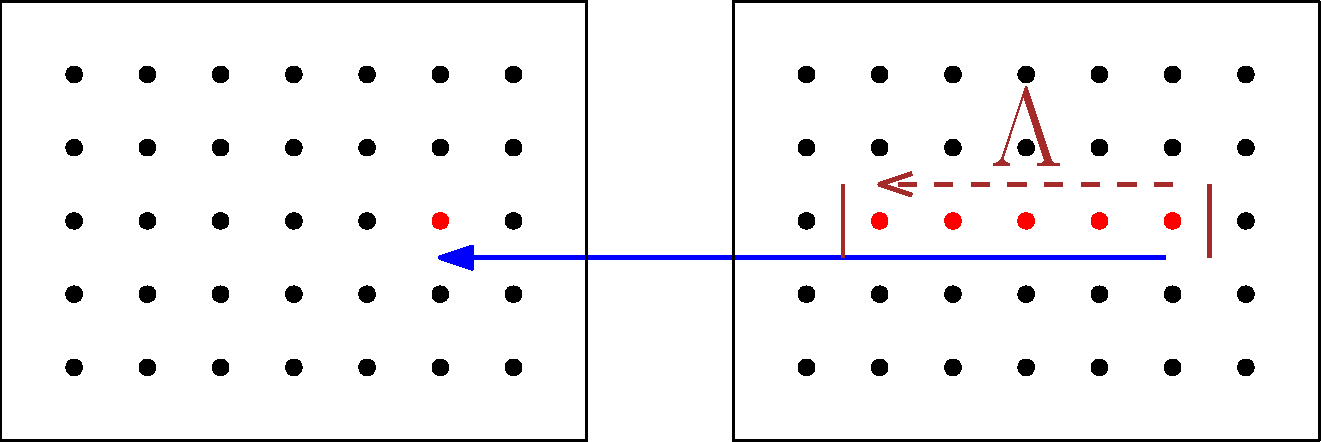
\includegraphics[width=1.0\textwidth]{chapters/litreview/images/stereo_matching-eps-converted-to.pdf}
    \caption{Diagram of the basic process of \gls{sm}. In this instance, for each pixel in the left image, a horizontal range of the pixels in the right image are searched, to find the one on the right that matches most closely to the one on the left. This has the effect that the \gls{disparitymap} is from the perspective of the left camera. The red dots represent the compared pixels. The brown dashed arrow and vertical bars represent the range of pixels in the right image to compute matching scores against. The length of the range is the lesser of the number of pixels before reaching the left border of the image, or the maximum \gls{disparity}, which is a parameter set by the user and represented here by \(\Lambda\).  Image from \cite{bsmpcvpic}.}
    \label{fig:stereomatchingbasic}
\end{figure}

% While precise approaches vary, the vast majority of \gls{sm} algorithms utilise some form of pixelwise comparison between images.  The basic process for this is shown in \autoref{fig:stereomatchingbasic}.    This comparison function be as simple as taking the absolute difference of the pixels under comparison.

In the general case \gls{sm} is impossible to perform perfectly because it is an ill-posed problem \cite{Gimelfarb1998}.  Going from a three-dimensional scene to a two-dimensional image necessarily involves a loss of information.  For any given image there are potentially an unbounded number of possible real-world scenes that could produce said image.  Using multiple images -- the more the better -- for \gls{sm} permits some recovery of information, but the process inevitably suffers from various sources of noise (where `noise' is defined broadly).

Liu \textit{et al.} \cite{Liu2005} describe four types of noise:  Signal, geometric, electronic and optical.  Signal noise arises from the normal operation of digital cameras, and electronic from differences between the internal operation of cameras used to capture images from different perspectives of the same scene.  Optical noise mainly stems from differences in the intensity and colour of light seen by the cameras at different perspectives when capturing images of the scene, caused by differences in the interactions between the objects of the scene and the available light sources at different points.  Lastly, geometric noise is a natural consequence of the fact that different perspectives must be used, and can be caused by issues as simple as the fact that points visible in one scene may not be visible in the other -- so-called `occlusions', caused by one part of the scene obscuring another part.

A key consequence of the last source of noise is the fact that, even in ideal circumstances with multiple `perfect' cameras, flawless lighting throughout the scene and \fxnote*{Provide reference for Lambertian surfaces}{objects which do not reflect light differently at different parts of their surfaces}, occlusions mean that for an arbitrary scene it is impossible to be certain a given algorithm has achieved a perfect reconstruction of the depths of the scene \cite{Gimelfarb1998}.  Strictly speaking, it \emph{is} possible that \gls{sm} produces an entirely accurate \gls{disparitymap}, but there would be no way to know without the use of additional information.

\fxwarning[inline,nomargin]{Include some example images to show the idea of stereo matching?}

\subsubsection{Image Rectification}
To reduce the computational complexity involved in performing \gls{sm}, many, perhaps most, algorithms only directly compare pixels along a single line in each image, typically the same horizontal line \cite[Ch. 11]{Szeliski2011}.  If the lines in the two images do not correspond to roughly the same part of the scene, then the matching process will likely fare poorly.  Such a discordance can occur when the cameras were not adequately aligned in terms of their spatial positions and angles relative to each other at the time of mutual image capture.

To overcome the challenges caused by mismatched lines, stereo image pairs are usually `rectified' (see e.g. \cite[Ch. 1.5.1]{Wohler2013}), wherein the captured images are adjusted so that they were effectively \fxerror*{Rectification could be described more precisely}{taken by properly aligned cameras}.  If rectification is performed well, the lines in the image should be properly aligned.  The parameters used in rectification in turn are deduced via camera calibration (see e.g. \cite[Ch. 1.4]{Wohler2013}), though neither topic is discussed further here.  For current purposes, all stereo image sets used are assumed to have been appropriately rectified already.

\begin{anfxnote}{}
    Discuss epipolar geometry?
\end{anfxnote}

\subsubsection{Middlebury}
\fxnote[inline,nomargin]{Talk about the Middlebury benchmarks, resources and website here.}

\subsubsection{Local vs Global}
\fxerror*{Expand/explain}{\cite{Scharstein2002}  (similar terms were in use earlier \cite{Gimelfarb1998})}

Perhaps the simplest and most obvious ways to perform \gls{sm} involve simply comparing the values of pixels in one image to the values of pixels in the other.

\subsubsection{\glsentrylong{mrf} \& Bayesian Inference}
\fxerror*{Expand/explain}{\cite{Kolmogorov2015,Blake2011}}

Not all global \gls{sm} algorithms utilise message passing, e.g. Graph Cuts \cite{Kolmogorov2001,Tappen2003}

Geman \& Geman \cite{Geman1984} showed that \glspl{mrf} are equivalent to Gibbs Distributions and that the two could be applied usefully to image tasks \cite{Gimelfarb1999}.

\begin{anfxwarning}{Pixel similarity measures}
    Move the below discussion about pixel similarity measures further up, probably into the \gls{sm} in general section?
\end{anfxwarning}

Frequently, in global methods the function used for the data cost is quite simplistic.  Most common is the use of simple absolute difference between the intensities of the pixels compared.  Other popular methods include \gls{sad} and \gls{ssd} \fxerror[inline]{[ref]}, adaptive window methods \cite{Yoon2005,Yoon2006}, and Birchfield \& Tomasi's Pixel Dissimilarity Measure \cite{Birchfield1998}.

In general, most \gls{mrf} approaches to \gls{sm} tend to use a truncated linear function to estimate the discontinuity/smoothness cost.  Such a function typically takes a form such as \[ E_{discontinuity} = \alpha \times min(| d_p - d_q |, \beta) \] where, for the purposes of this equation, \(E_{discontinuity}\) represents the total estimated cost of the assignment; \(\alpha\) is a scaling coefficient that may or may not be used; \(\beta\) is a constant that provides the upper limit to the cost estimate; and \(d_p\) and \(d_q\) are the proposed \fxwarning*{labels?}{labels} of the current pixel and its neighbour currently under consideration.  While a simple absolute difference function is perhaps the most common applied to the labels, it is important to note that it is not the only one that could be used.  

For example, Ha and Jeong \cite{Ha2016} use a two-step \fxnote*{Define Potts model}{Potts model}, with different penalties for a difference of 1 compared to a difference of 2 or greater. Conversely, Tan \textit{et al.} \cite{Tan2017} comment that a typical Potts function can be viewed as a special case of the absolute difference truncated linear function, where the truncation value (\(\beta\) in the equation above) is 1, while the coefficient is the value of the Potts penalty parameter.

The choice of the truncated linear function is motivated by the assumption that most surfaces in images either are planar, or smoothly vary in disparities, and thus larger jumps should be penalised more heavily, but very large jumps are almost certainly indicative of an object boundary where a large difference in disparities is warranted.  Therefore, at a certain point, the penalty to assign significantly different values should stop growing, so as not to reduce the likelihood of correctly assigning large differences in disparities at object edges.

\subsection{Dynamic~Programming}

\gls{dpsm} was first introduced by Gimel'farb, Marchenko and Rybak in 1972 \cite{Gimelfarb1972}.\footnote{There is a popular misconception that \gls{dpsm} was introduced in the 1980s with \cite{Ohta1985}.  This is plainly false, given that \gls{dpsm} was first described years earlier.  The confusion is unsurprising, however, because \cite{Ohta1985} was likely the first description of \gls{dpsm} many in the English-speaking world saw, as a consequence of the Cold War.  For example, the authors \cite{Salmen2009} of seem to have this misunderstanding.}  

% \begin{anfxnote}{DP's streaking}
%     Be sure to mention the streaking commonly seen with \gls{dpsm} -- if nothing else it will be important for explaining why \gls{sgm} was created.
% \end{anfxnote}

Anecdotally, variants of \gls{dpsm} are still popular in practical applications of \gls{sm} because it tends to give acceptable results \fxerror[inline]{[ref?]} and is amenable to fast implementations with low-powered devices \fxerror[inline]{[ref?]}.

\begin{anfxnote}{Why mention DP?}
    Partly because it is a basis for other algorithms, but at least as much because the process of propagating information up and down the scanlines that it entials is very much reflective of message passing.  ``The main difference between DP and 1D BP is the word `message' '' -- Georgy (at my provisional).  Something similar was mentioned in appendix B to \cite{Szeliski2011}.
\end{anfxnote}

\subsubsection{Symmetric Dynamic Programming Stereo}
Motivated by observations of the physical reality of the image capture process and propounded by Gimel'farb \fxerror*{Expand/explain}{\cite{Gimelfarb1979,Gimelfarb2001} + \cite{Nguyen2013,VanMeerbergen2001}.  \cite{Khan2016}}

\subsection{\glsentrylong{bp}}
\gls{bp} was introduced by Pearl \cite{Pearl1982} for use with inference engines, in the context of Bayesian Statistics \fxerror[inline]{[ref]} and Gibbs Distributions \fxerror[inline]{[ref]}.  \gls{bp} was first applied to \gls{sm} in \cite{Sun2003} where it demonstrated excellent matching performance compared to many contemporary matching algorithms, but the `breakthrough' paper was arguably \cite{Felzenszwalb2006}, where a near-real time implementation was presented which still had extremely good results.  Szeliski commented in c. 2011 that \gls{lbp} was still used at that time in some of the best-performing \gls{sm} algorithms \cite[p. 163]{Szeliski2011}.

\begin{figure}
    \centering
    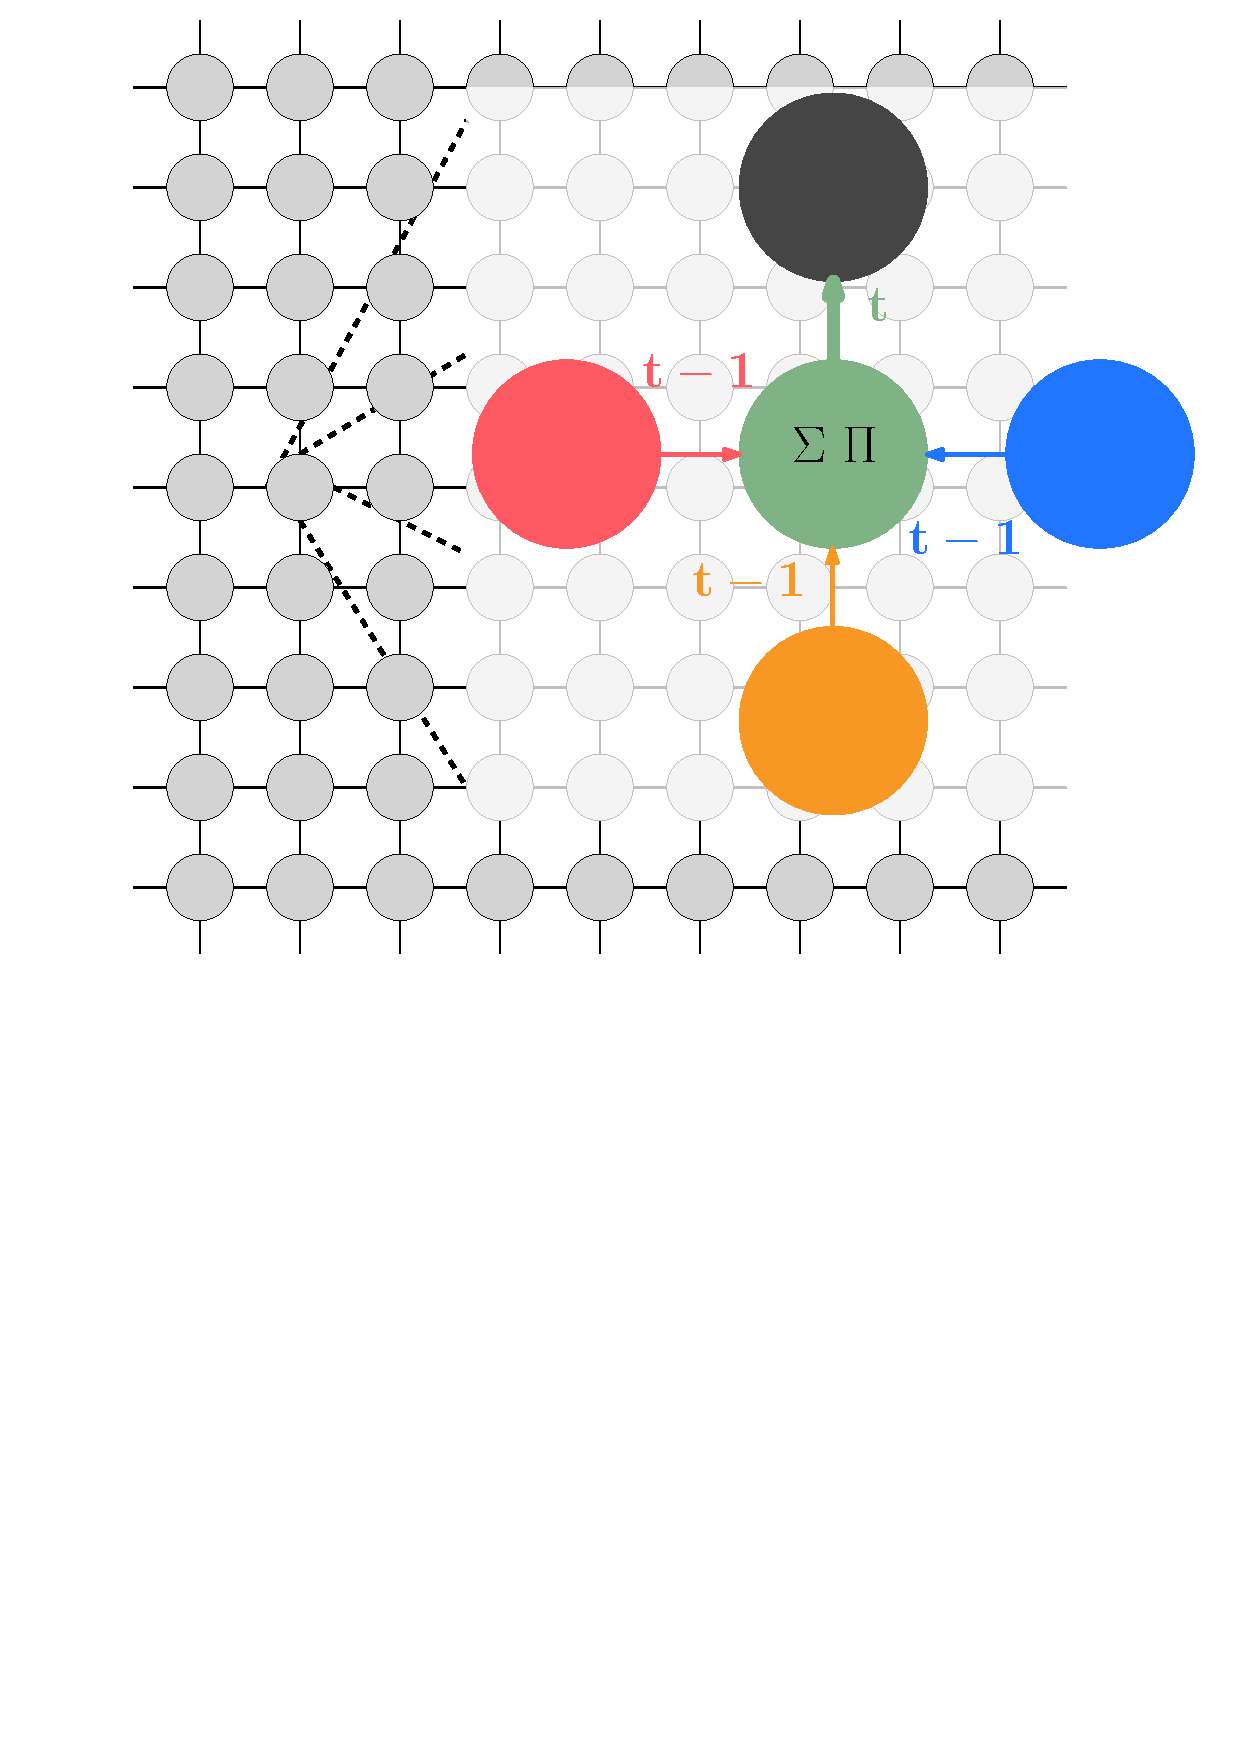
\includegraphics[width=1.0\textwidth]{chapters/litreview/images/bp_diagram_recoloured.pdf}
    \caption{Pictorial representation of the concept behind Loopy Belief Propagation for Stereo Matching. The symbols in the central cell refer to sum-product Belief Propagation, one of the earliest and mostly widely discussed forms of Belief Propagation. Each cell sends a new message to its neighbouring cells at each iteration after in turn having received and processed new messages from the neighbours in the previous iteration. The outgoing message to a given neighbour is computed from the information received from the other neighbours previously, represented here by the three thin and one fat arrow.  Image from \cite{lbpmpsmpic}.}
    \label{fig:bpdiagram}
\end{figure}

Yang \textit{et al.} \cite{Yang2006a} built upon \fxerror*{Explain hierarchical BP}{hierarchical \gls{bp}}, adding in extra steps before and after the \gls{bp} process.  They combine information derived from using the mean shift algorithm \cite{Comaniciu2002}; a colour-weighted correlation method based on Yoon \& Kweon's \cite{Yoon2006} applied to both the left and right images; a left-right consistency check to detect occluded pixels; a plane-fitting process based on Tao \& Sawhney's \cite{Tao2000}; as well as \gls{bp} itself.  While combining these various techniques leads to a highly-accurate disparity map,\footnote{This algorithm achieved the top ranking on Middlebury when it was first introduced.} this approach is \emph{extremely} slow.

Typical \gls{bp} uses the four-connected neighbourhood to define the neighbours of each given node in the grid.  This means that each node passes messages to and from it's immediate neighbours up, down and to the left and right of it in the grid.  Other neighbourhood arrangements are possible though, depending on the underlying model one wants to use.  For example, Tan \textit{et al.} \cite{Tan2017} describe an approach to \gls{bp} where every pixel is considered to be a neighbour of every other pixel.  Messages are weighted according to the distance across the grid between the neighbours, with nearer neighbours having a greater impact upon a pixel's final beliefs.  The major advantage of this approach is that it almost eliminates the need for repeated iterations of message passing.

Ha and Jeong \cite{Ha2016} suggested a different approach for scheduling the messages.  Instead of each pixel repeatedly exchanging messages with its neighbours until a reasonable amount of the grid has been spanned, they start in one of the corners in the image, and sequentially pass messages along two directions until reaching the other corner, repeating this process once for each corner.  The great advantage of this is that in principle one only needs to perform message exchanges in each direction once.  Their implementation still required roughly \SI{3.5}{\second} to complete, however, without returning a significantly more accurate disparity map.\footnote{The authors claimed that their method was \numrange{300}{600} times faster than `standard` \gls{bp}, but they did not specify their stopping condition.  Based on their reported results it appears that they used well over 300 iterations on an image with their standard comparison -- many more than would be reasonable for image sizes likely to be targeted for real-time \gls{sm}.}

Balossino \textit{et al.} \cite{Balossino2007} suggested an alternative formulation to the traditional grid of \gls{lbp}.  Instead, they built a forest of trees, each of which was rooted at the given pixel under consideration, and which has a handful of neighbouring pixels as children.  The attraction of this approach is that it restores the properties of optimality and convergence described in \cite{Pearl1982} for one round of messages up and down each tree.  This advantage is tempered, however, by the necessity of combining results from different trees.  The final accuracy appeared to be worse than with \cite{Felzenszwalb2006}, and there was no reporting of the running time, though it seems unlikely that this approach was fast.

It should be noted that \gls{bp} is \emph{not} regarded as the current top-performing \gls{sm} algorithm.  Tippets \textit{et al.} found c. 2012 that, of algorithms implemented on the CPU, SADL from \cite{VanDerMark2006} was the fastest accurate-enough method, and ADCensus from \cite{Mei2011} was the most accurate, and in fact was described as ``Pareto-optimal'' by Tippets \textit{et al.}  \fxnote{Move this paragraph?}  In terms of \gls{gpu} implementations, the algorithm from \cite{Zhao2011} was the fastest by far (though it only properly worked when observing scenes with motion).  The authors do not state an overall most-accurate \gls{gpu}-based algorithm, but based on Fig. 7 in \cite{Tippetts2016}, it appears that the \gls{gpu} implementation of the ADCensus algorithm from \cite{Mei2011} was again the best.\footnote{Other, faster, algorithms were also discussed, but those required specialist hardware such as \glspl{fpga} or \glspl{dsp}.}  \Gls{bp} \emph{is} amenable to parallelisation (unlike its traditional rival, Graph Cuts \cite{Tappen2003}) and \gls{gpu} implementations, but the main point of interest for it in this work is the fact that it is explicitly built around the concept of independent processing elements exchanging messages.

\begin{anfxwarning}{Top algos on Middlebury}
    Thinking about it, I probably should investigate the current top-performing algorithms on Middlebury, at least the ones which have accompanying publications.
\end{anfxwarning}

\subsubsection{Real-time/resource-constrained \glsentrylong{bp}}
One of the major drawbacks of \gls{bp} as compared to a number of other approaches to \gls{sm} is that a simple naïve implementation is both quite slow, and very memory-intensive.  Slow because of the requirement to perform many iterations, and memory-intensive because \emph{at least} one copy of the data costs and the message estimates for each neighbour must be stored in memory, with the result that a number of values on the order of at least \(O(5XYD)\) are kept in memory, where X and Y are the width and height of the stereo images, and D is the size of the disparity range.

Seeking to derive the comparative benefits of a global stereo algorithm without compromising resource and time requirements too much, there have been a number of attempts at a real-time \gls{bp} algorithm \cite{Liang2011,Perez2010}.

Felzenszwalb \& Huttenlocher \cite{Felzenszwalb2006} made three significant improvements:  i) They demonstrated a way to reduce the complexity of the message update process from \(O(|D|^2)\) to \(O(|D|)\) (where \(|D|\) is the total number of potential disparity labels).  ii) They showed that, because each pixel relies entirely upon the messages received from its neighbours at the previous iteration, only half of the pixels in fact need to be updated in a given iteration, without affecting the final results.  This both halves the number of message computations required for each iteration, but moreover means that only a single copy of the messages need be kept while ensuring that messages computed earlier in an iteration have no impact upon messages computed later.  iii)  They introduced a hierarchical approach, where the first iterations were performed over a much smaller grid, representing an amalgamation of the actual grid, but later iterations would operate over larger and larger grids until reaching the full size.  This had the benefit of propagating information across the grid in a much faster fashion, with relatively little loss in accuracy.  Almost every claimed real-time \gls{bp} algorithm since uses the hierarchical approach.

Notably, Tippetts \textit{et al.} characterised the final algorithm implemented in \cite{Felzenszwalb2006} as Pareto-optimal against almost all other CPU-based \gls{sm} algorithms that they examined, suggesting that there were only five others which provided either better accuracy \emph{or} faster runtimes.  Of course, in the meantime there likely have been improvements in both metrics by newer algorithms.

Yang \textit{et al.} \cite{Yang2006} claimed that they had devised a new approach that would provide a 45x speedup, and boasted that their system could achieve a frame rate of 16 \gls{fps} on a 320 x 240 image with 16 disparity levels.  This claim was largely based, however, in the fact that they used a \gls{gpu} to implement it -- but later stated that they had not yet implemented their method on a \gls{gpu}.  Furthermore, they did not present anything conceptual that had not already been described in \cite{Felzenszwalb2006}. %by Felzenszwalb \& Huttenlocher.

Yu \textit{et al.} \cite{Yu2007} presented a proposed approach for compressing the messages, thus reducing total memory occupied, but it has not proven popular.  This may be because it is not amenable to parallelisation, thus significantly reducing its practicality \cite{Yang2010}.

Yang, Wang \& Ahuja \cite{Yang2010} proposed an approach which they claim needs only constant memory space, regardless of the number of disparities involved, while still returning results that are almost as accurate.  For example, they claim that for an image with 800 x 600 pixels and 300 disparity levels, their algorithm requires only around \SI{9}{\mebi\byte} of memory --- though it is not clear though whether they include storing the computed data costs in that amount or not.  The main element of their approach is that as they move from the coarser levels of the hierarchy, they proportionally reduce the number of disparity labels considered at each level, keeping the total memory required constant.  %This leads to an issue in that, should the true disparity not be selected for inclusion at a reduction, that pixel will never see the correct disparity label assigned to it.  To work around this, they 

Gupta \& Cho \cite{Gupta2012} used 3x3 tiles in their hierarchical method, rather than the usual 2x2.  This meant that their process was somewhat faster overall, and means that at the more coarse levels they need less memory.  The other main differences between their method and previous ones are that they use an `alternative schedule method' borrowed from \cite{Tappen2003}; and they use a different disparity refinement operation as final step.  The results, in terms of accuracy and speed, do not appear to be any better than earlier papers, though.

Xiang \textit{et al.} \cite{Xiang2012} also boasted of a new technique that enabled faster speeds, but again their implementation largely merely borrowed concepts from \cite{Felzenszwalb2006} and used a \gls{gpu}.  They did improve accuracy results, however, by incorporating Yoon \& Kweon's \cite{Yoon2005} adaptive support-weight approach as a post-processing step, with minimal extra computational requirements.

Tan \textit{et al.} \cite{Tan2017} claim that their fully-connected \gls{bp} method is highly-amenable to parallelisation, suggesting it could be implemented to run in real-time, but they do not appear to have done so themselves.

\subsection{\glsentrylong{sgm-glossary}}
This won't really be touched upon in this work anymore, but it might be a good idea to mention/describe it (and perhaps \gls{cp} too), if just so I can mention it again as an obvious future work target.

% \subsection{Noise-Driven Concurrent Stereo Matching}


% \subsection{\label{subsec:concprop}\glsentrylong{cp}}

% \cite{Gong2015,Gong2013a}

% \subsection{Message Passing \glsentrytext{sm} -- other?}
% Look at, e.g.:
% Tan, X. et al. (2017) ‘Efficient Message Passing Methods With Fully Connected Models for Early Vision’, IEEE Transactions on Image Processing, 26(12), pp. 5994–6005. doi: 10.1109/TIP.2017.2750406.
% Ružic, T., Pižurica, A. and Philips, W. (2011) ‘Neighbourhood-consensus message passing and its potentials in image processing applications’, in Astola, J. T. and Egiazarian, K. O. (eds) Image Processing: Algorithms and Systems IX. San Francisco: Society of Photo-Optical Instrumentation Engineers, p. 78700Z. doi: 10.1117/12.872464.
% Ružić, T., Pižurica, A. and Philips, W. (2012) ‘Neighborhood-consensus message passing as a framework for generalized iterated conditional expectations’, Pattern Recognition Letters, 33(3), pp. 309–318. doi: 10.1016/j.patrec.2011.10.014.
% Szeliski, R. et al. (2008) ‘A Comparative Study of Energy Minimization Methods for Markov Random Fields with Smoothness-Based Priors’, IEEE Transactions on Pattern Analysis and Machine Intelligence, 30(6), pp. 1068–1080. doi: 10.1109/TPAMI.2007.70844.
% Thomas, D. et al. (2019) ‘Revisiting Depth Image Fusion with Variational Message Passing’, in 2019 International Conference on 3D Vision (3DV). IEEE, pp. 328–337. doi: 10.1109/3DV.2019.00044.


\chapter{\label{chap:back}Background}
% This review of past work focuses on the main areas of Computer Science that are relevant to this dissertation.  In none of these cases does the review come close to comprehensively covering the entire span of the given area.  It merely tries to cover as much of the relevant recent and classic work as possible, while giving an extremely brief introduction to these areas.  The interested reader who is unfamiliar with any of these topics is strongly advised to refer to the materials cited.

This \lcnamecref{chap:back} summarises some pertinent related topics that are relevant to the central body of this dissertation.  Each is only a short summary, sufficient to communicate key ideas, provide necessary background information, and demonstrate that there are almost always multiple related theoretical concepts and approaches to solving problems.  In none of these cases does the synopsis come close to comprehensively covering the entire span of the given area.  Each part merely tries to introduce and illuminate its topic sufficiently for the purposes of this work.  The interested reader who is unfamiliar with any of these topics is strongly advised to refer to the materials cited.

% See \url{http://forneylab.org/} for something seemingly quite similar to what I'm doing...;  fglib \url{https://github.com/danbar/fglib};  IGraph library \url{https://igraph.org/};  LGNpy \url{https://github.com/ostwalprasad/LGNpy};

This \lcnamecref{chap:back} specifically discusses formal models of concurrent computation, synchronous \& asynchronous communication, \gls{cml} and \gls{mc}.  \Gls{mc} is, in fact, another model of concurrent computation, but given its central position in this work, it is given a dedicated separate \lcnamecref{sec:back:mc}.  The same can be said about \gls{cps}, which is given its own \lcnamecref{chap:tsp}.

\section{\label{sec:back:formalmodels}Formal Models of Concurrent Computation}
The models briefly reviewed in this \namecref{sec:back:formalmodels} are just a small sample of the formal models for computation that have been devised.  An important aspect of each of the ones mentioned below is that they explicitly deal with concurrency in some fashion, thus meriting their (severely abridged) discussion.  Ultimately, \gls{mc} is used as the model of choice for the remainder of the dissertation after this \namecref{chap:back}, but it undoubtedly has been influenced by, or developed contemporaneously with, each of the below.  Indeed, close study of each model inevitably reveals commonalities between them.

\subsection{\label{subsec:back:csp}Communicating Sequential Processes}

\emph{\Gls{csp}} is a \emph{process algebra} and abstract model of concurrent computation put forward by Hoare \cite{Hoare1985,Roscoe2011}.  A typical sequential computation is represented by a \emph{process}.  Processes' \textcquote[][p.~478]{Roscoe2011}{behaviour is described in terms of the occurrence and availability of abstract entities called \textit{events}}.  Should more than one event be available simultaneously for a given process, then one will be chosen non-deterministically.  This choice is internal to the process, and not influenced by, or visible to, other processes.

Concurrency is introduced by the existence of multiple processes.  In general, the processes continue independently, responding to events as they come.  Should a particular event appear in the alphabet of multiple processes, however, then all processes \emph{must} choose to participate in that event at the same time.  Should all processes involved make such a choice, they engage in a synchronous multi-way atomic synchronisation (hence ``communicating'').  \Gls{csp} has provided significant inspiration for concurrency design in a number of programming languages, notably including Ada \cite{Defense1983,Taft2013}, Occam \cite{Elizabeth1987}, Google's Go \cite{Meyerson2014} (not to be confused with the earlier language Go! \cite{Clark2004}, which itself was explicitly designed for concurrency) and \gls{cml} \cite{Reppy2011} (see further \vref{sec:back:cml}).  An especially interesting practical application of \gls{csp} itself is finding flaws -- and fixes to the flaws -- in information security protocols \cite{Roscoe1995,Lowe1996,Koltuksuz2010}.

\subsubsection{\(\pi\) Calculus}
\(\pi\) calculus was created by Robin Milner and associates in the early 1990s, building upon \gls{csp}.  Milner appreciated \gls{csp}, which advanced concurrency models by explicitly incorporating \emph{synchronised} interaction, something his earlier Calculus for Communicating Systems \cite{Milner1980} had lacked  \cite{Milner1993}.  Milner still regarded \gls{csp} as incomplete, however, in that it had no support for the concept of `mobility' --- \ie{} the ability of the system to reconfigure itself during operation.  In the context of \(\pi\) calculus, this is achieved by passing references to links between processes via other links, thus enabling a dynamic communication system. \(\pi\) calculus was created as an attempt to build upon earlier systems but present a complete calculus of concurrent computation, in much the same way that Lambda Calculus \cite{Barendregt1984} is a complete calculus for sequential computation.\footnote{Milner also noted that sequential computation is a special case of concurrent computation \cite{Milner1993}.}

Both \gls{csp} and \(\pi\) calculus are effective for modelling concurrent systems (see \eg{} \cite{Roscoe2011}).  They have a drawback, however, in that they tend to be very verbose.  Specifications of behaviour for processes are intertwined with the descriptions of processes' states.  They are effective for specifying a system formally, and verifying the behaviour of said system by defined reductions (see \eg{} \cite[Ch.~3.2]{Varela2013}), but for larger systems the notational burden can make it difficult to understand what each process can and will do.

\subsection{\label{subsec:back:actors}\texorpdfstring{\Glspl{actor}}{Actors}}
The \emph{\gls{actor}} model was introduced by Carl Hewitt \cite{Hewitt1973} and substantially further developed for practical programming use by Gul Agha and others \cite{Agha1986,Agha1997}.  Much like \gls{csp} \& its cousins, the \gls{actor} model is based around the concept of sequential, separate but communicating processes which exchange messages.  Again, the processes make decisions independently and proceed based on their communications.  A key difference, however, is that in the \gls{actor} model the message exchanges are \emph{asynchronous}.  Each \gls{actor} has its own \emph{mailbox}, and may send messages to other \glspl{actor} so long as it knows their identity (which is equivalent for this purpose to a concept of a postal address for the \gls{actor}), \emph{but does not wait at all for a response before proceeding}.  Moreover, for \glspl{actor}, the \emph{only} way to communicate with one another is to know the intended recipient's identity/address.  Logical shared memory is explicitly disallowed,\footnote{It is entirely possible in practice, of course, to implement an \gls{actor} system on a shared memory system, but the model expressly forbids any notion of a resource shared in any fashion besides \glspl{actor} requesting a result from another \gls{actor} who has exclusive access to the resource.} which prevents changing who an \gls{actor} communicates with simply by \eg{} changing the holder of a channel endpoint, but also means that actors can be distributed by a runtime without (directly) affecting the practical programming.

The \gls{actor} model is popular for concurrent programming, possibly owing to its intuitive concept.  The fact that communication is asynchronous makes \glspl{actor} much more suitable for modelling distributed systems without shared memory than \gls{csp} or similar --- \glspl{actor} can send messages and proceed without (necessarily) needing to wait for a response, instead continuing forward based on the messages they have received.  By contrast, a typical distributed system with synchronous communication would have prohibitive time costs, given the relative slow speed of typical links between distributed computers as compared to their capacity for local processing.  Many \gls{actor} systems have been implemented for different programming languages (\eg{} \cite{Varela2001,Srinivasan2008,Charousset2016,Bernstein2016}), and in fact it is a core component, and perhaps largely responsible for the success, of Erlang/OTP \cite{Armstrong2010,Armstrong2013,Vinoski2012}.  A relatively new language, Pony \cite{Clebsch2015,Clebsch2017}, takes this even further.

\Glspl{actor}, when used for non-trivial real-world software, have been criticised at times \eg{} \cite{Welsh2013,Stucchio2013}.  While some of the criticisms described are implementation-specific (relating to Akka, a Scala \gls{actor} library), a common thread is that \glspl{actor} do not compose well.  This has the negative consequence that it is difficult to combine an \gls{actor} with anything else to create a new abstraction, and can require extensive modifications in source code to make relatively simple logical changes.

\subsection[GAMMA, the Chemical Abstract Machine, and Join Calculus]{\(\Gamma\), the Chemical Abstract Machine, and Join Calculus}

\subsubsection{\(\Gamma\)}
\citeauthor{Banatre1993} \cite{Banatre1993}, described the \(\Gamma\) (\emph{GAMMA}) ``language'', which uses the multiset as its singular data structure.  The originators stated that their goal with \(\Gamma\) was to create a \enquote{a program structuring tool} focusing on \enquote{logical parallelism} (which seems to be their name for concurrency), rather than creating a working programming language.  Indeed, they acknowledged that translating multiset transformations into programs working on existing electronic computers of the time may prove challenging.  The principal aim was to provide a facility for program designers to state at a high-level the intended transformations, avoiding imposing any ordering on the processing and instead permitting as much concurrency as possible:  \textcquote[][p.~102]{Banatre1993}{our high level of abstraction eliminates unfortunate sequential biases.}  In essence, \(\Gamma\) takes an extreme declarative approach.

Perhaps the largest drawback of \(\Gamma\) is its lack of any form of central control.  All computation is performed through local operations, while \textcquote[][p.~108]{Banatre1993}{the only known solutions to certain problems rely on control decisions involving the whole state of the computation.}  The first problem of such that \citeauthor{Banatre1993} point to is the \gls{gcp} (which is solved in linear time in \cref{chap:gcol} in the present dissertation).  While such problems \emph{can} be solved, expressing the solutions would likely be more, rather than less, complicated than in other systems.  Another criticism that can be levelled at \(\Gamma\) is its lack of formality around its data structure.  Multisets are used, but there is no clear foundation underpinning them.  Rather, in \cite{Banatre1993} both integers and tuples are used as the set elements without any consideration of how they might be constructed or represented.  This is probably appropriate for the extreme high level of \(\Gamma\), but it could impede conversions of its programs to lower level languages more suited to working implementations.

\subsubsection{The Chemical Abstract Machine}
\citeauthor{Berry1992} devised the idea of the \emph{\gls{cham}} \cite{Berry1992}, directly inspired by the concepts from, and building upon, \(\Gamma\).  The parallels between the \gls{cham} and \gls{mc} are clear.  Indeed, the \gls{cham} includes a concept of \glspl{compartment} created by membranes.  Moreover, in his foundational exposition of \gls{mc} \cite{Paun2000}, \citeauthor{Paun2000} directly cites \(\Gamma\) \cite{Banatre1988} and \gls{cham} \cite{Berry1992}.

\(\Gamma\) had a loose notion of being rooted in chemistry, but \gls{cham} significantly adds to the rigour of the analogy, introducing concepts such as molecules composed of atoms, where a system is a collection of such molecules and may be heated or cooled to change the molecular composition.  Where \cite{Banatre1993} made clear the potential of multiset transformations for concurrency, \cite{Berry1992} adds formalisms that enable much more precise specifications of the process of the transformations, without sacrificing the extreme levels of concurrency possible.  The authors demonstrate this fact by showing that \glspl{cham} \enquote{can implement known models of concurrent computation}, including CCS \cite{Milner1980}, mobile processes \cite{Milner1991} and concurrent lambda calculus \cite{Boudol1989}.

\subsubsection{Join Calculus}
Where the \gls{cham} was a development of \(\Gamma\), join calculus is in turn a development of the \gls{cham}.  Join calculus -- created in the 1990s by \citeauthor{Fournet1996} \cite{Fournet1996,Fournet2002} and using the \gls{cham} as its underlying ``machine'' (although, it actually originally targeted \(\pi\) Calculus before switching to the \gls{cham} as a much better fit for its core concepts \cite{Fournet2002}) -- is arguably the most similar in practice of all the models discussed in this \namecref{sec:back:formalmodels} to \gls{mc}.  There are clear common elements between join calculus and \gls{cps}, including heavy use of pattern matching and communication via channels.  Even its reaction rules closely resemble the typical style of rules found in most flavours of \gls{ps} (see \cref{sec:back:mc,chap:cpsystems}).

\citeauthor{Fournet2002} specifically describe join calculus as \textcquote[][p.~269]{Fournet2002}{an attempt to provide language support for asynchronous, distributed, and mobile programming.}  Join calculus has proved fruitful for assisting in the design of new concepts in practical programming, including JoCaml \cite{Fournet2003} (essentially an implementation in OCaml of join calculus as a programming system), Joinads \cite{Petricek2011}\footnote{See also \url{http://tryjoinads.org/docs/use/joins.html}.} and Reagents \cite{Turon2012}.  Despite this utility, however, join calculus seems largely to have been neglected by those outside the theoretical computer science and programming languages communities and appears to have been entirely unused in more recent years.  Later work building on this dissertation could well benefit from an attempt to use join calculus, but it appears less likely to be immediately fruitful than using \gls{mc}.

\subsection[Brane- and Kappa-Calculus]{Brane- and \(\kappa\)-Calculus}
\subsubsection{Brane Calculus}
Brane Calculus\footnote{\citeauthor{Cardelli2005} actually referred to it as Brane \emph{Calculi}, given that he saw it as a family of related systems, but Calculus is used here for consistency with the other described models.} might appear, \foreign{prima facie}, to be the closest relative to \gls{mc} of all the models presented in this \namecref{sec:back:formalmodels}.  The subtitle given to its exposition is \enquote{Interactions of Biological Membranes} \cite{Cardelli2005}.  Both models are undeniably grounded in concepts of cellular biology, with particular emphasis on the cell's membranes.  Both focus heavily on the nesting of those membranes, and movement of items among them.  In actuality, they are dissimilar.

Brane Calculus is as much a system for modelling certain biological processes as it is a computational system.  Importantly, it means that the primitives chosen for it are relatively biologically realistic, and likely much more feasible to implement physically using biology.  While that has some clear potential benefits, it also tends to make even relatively simple systems somewhat difficult to follow.

Brane Calculus also treats its membranes somewhat differently.  In \gls{mc} (certainly \gls{clps}, at least), membranes are used primarily to separate regions of computation and avert undesired interactions between the contents of \glspl{compartment}.  In Brane Calculus, however, much of the processing occurs \emph{on} the membrane itself: \textcquote[][p.~257]{Cardelli2005}{Membranes are not just containers, they are coordinators and active sites of major activity.}  Brane Calculus seems like a promising potential target for an ``intermediate language'' in between \gls{ps} and real biological implementations, but also seems much less useful for expressing the core essence of general computations than \gls{mc}.

\subsubsection{\(\kappa\)-calculus}

Similarly to Brane Calculus, \(\kappa\)-calculus \cite{Danos2004} was introduced as a formal representation of an aspect of cellular biology grounded in prior work in theoretical computer science on concurrent languages.  The focus in \(\kappa\)-calculus is predominantly upon protein interactions, rather than membranes as with Brane calculus: \textcquote[][p.~70]{Danos2004}{Our language idealizes protein-protein interactions, essentially as a particular kind of graph-rewriting}.  This protein focus is demonstrated in \cite{Danos2004} with an example describing part of the digestion process that occurs inside \textit{E.Coli} bacteria, the \enquote{lactose operon}.

The development of \(\kappa\)-calculus may have remained more firmly grounded in traditional concurrency theory than Brane Calculus.  Notably, \citeauthor{Danos2004}, in \textcquote[][p.~76]{Danos2004}{a side observation perhaps only of interest for Concurrency theorists} comment upon their use of \enquote{the ordinary material of process algebras}, pointing out that they use only a minimal subset of the usual operations.  Furthermore, they demonstrated that their simpler (in terms of allowed protein reactions) language \(m\kappa\)-calculus could simulate \(\pi\) calculus, meaning that they could translate systems created in \(\kappa\)-calculus to \(\pi\) calculus and then use programmatic implementations of \(\pi\) calculus, such as Nomadic Pict \cite{Unyapoth2001}, to run those systems on electronic computers.  While this shows that \(\kappa\)-calculus could be used to model solutions to arbitrary problems, it still suffers from the same problem as Brane Calculus.  The modelling for even relatively simple systems quickly becomes quite complex and difficult to read, diminishing the utility of \(\kappa\)-calculus for exploring alternative solutions to known problems in computer science.

\subsection{\label{sec:back:othermodels}Other Models}

\subsubsection{Petri Nets}
Perhaps the earliest formalised model of concurrent computation still in wide use is the \emph{Petri net} \cite{Dennis2011}, first conceived of by Carl Petri to describe chemical processes \cite{Petri2008}.  A basic Petri net consists of places, tokens and transitions, where tokens move between places via arcs and all places are separated by transitions (and \viceversa).

The main weakness of classical Petri nets is that they require the definition of a fixed system from the outset, and do not easily permit the evolution of the system during ``runtime'' as appropriate.  Of Petri nets, \citeauthor{Varela2013} says \textcquote[][p.~36]{Varela2013}{Petri nets \textelp{} in the \textelp{} form described \textins{in \cite{Varela2013}}, \textelp{} are not able to model the dynamicity of concurrent software\textins{.}  \textelp{} Petri nets \textelp{} do not support the compositional reasoning afforded by more modern models of concurrency.}

\subsubsection{\label{sec:back:pram}Parallel Random Access Machines}

\emph{\Glspl{pram}} are a model for concurrent computation arguably closer to the operation of real electronic computers than the others described above.  \citeauthor{JaJa2011} defines a \gls{pram} as \textcquote{JaJa2011}{an abstract model for parallel computation which assumes that all the processors operate synchronously under a single clock and are able to randomly access a large shared memory. In particular, a processor can execute an arithmetic, logic, or memory access operation within a single clock cycle}.  Unlike the process algebras described above, the \gls{pram} model does not, in general, impose a particular way to describe a \gls{pram} algorithm, making it sometimes quite seful in developing parallel algorithms.

\Glspl{pram} developed as a natural extension to random access machines (RAMs), which, as the name suggests, provide a model that is reasonably close to typical uniprocessor electronic computers.  A \gls{pram} is a collection of processors operating synchronously (\ie{} on the same clock), each labelled with a unique identifier, and with access to a global shared memory.  Processors may operate independently of each other, but many described \gls{pram} algorithms in fact operate in a \emph{single-program multiple-data} fashion where all processors follow the same program and so are only semi-independent, at best.  These attributes mean that a \gls{pram} often looks quite similar (at a superficial level, at least) to the operation of a typical \gls{gpu}.  The systems described in \cref{chap:nmp} also bear more than a passing resemblance to \glspl{pram}.
%-------------------------------------------------------
\section{\label{sec:back:syncasync}Synchronous and Asynchronous Messaging in Distributed Algorithms}
%-------------------------------------------------------

This dissertation uses the standard timing models in distributed algorithms \cite{Lynch1996} for messaging where relevant.  For reference, the most important relevant concepts are explained and illustrated below.  For more on the topics discussed in this \namecref{sec:back:syncasync}, the interested reader is referred to \cite{Fokkink2013,Lynch1996,Tel2000}.

\subsection{Rounds}
Under both synchronous and asynchronous messaging, all processes work in \emph{rounds} (sometimes also referred to as \emph{macro-steps}).  A round consists of three repeating sequential sub-steps:
\begin{enumerate}
    \item \emph{\textsf{Receive}}:  receive one or more incoming messages
    \item \emph{\textsf{Process}}:  perform any requisite local computations as induced by the received messages, and update the local state
    \item \emph{\textsf{Send}}:  send out new messages as appropriate based on the processing from the previous step
\end{enumerate}
This applies only to messaging between processes.  For systems with a solitary process, there is no meaningful concept of rounds because the process will essentially remain in the \textsf{process} sub-step.  \Ie{} a lone process will continue working without messaging until the system halts (if ever).

\subsection{Synchronous Messaging}
Under the synchronous model, all processes proceed in lock-step.  They may carry out the sub-steps at different speeds, but begin and end rounds together.  When considering timing of messaging, there are two standard approaches:  to consider the \textsf{process} sub-step as taking one time unit and the transit time -- the time between when the message is sent by the sender and when it is received by the recipient -- taking zero time units; or, to consider the \textsf{process} sub-step as taking zero time units and the transit time taking one time unit.

\subsection{Asynchronous Messaging}
Under the asynchronous model, there is (unsurprisingly) no natural synchronisation between processes.  All processes proceed through the sub-steps at their own pace.  The \textsf{process} sub-step is considered to take zero time units, and message transit times are considered to take any number of time units.  Alternatively, by normalisation, while the \textsf{process} sub-step still takes zero time units, message transit times take somewhere between zero and one (inclusive) time units.  This makes the second synchronous approach a special case of the asynchronous approach.  The asynchronous model is similar to the theoretical \gls{actor} model.

\subsection{Echo}
To illustrate the difference between the synchronous and asynchronous scenarios, consider the illustrations in \cref{fig:back:echosync,fig:back:echoasync}.\footnote{These figures were created by Dr. Radu Nicolescu, and have been reproduced here with his permission.}  The \textsf{echo} algorithm \cite[Ch.~4.3]{Fokkink2013} is used to establish a spanning tree over a graph of nodes/processes, in this case rooted at node 1.  The algorithm works in two phases, named \emph{broadcast} and \emph{convergecast}.  \textsf{Echo} starts in the broadcast phase with an initiator node sending out a broadcast message to each of its neighbours.  Each of those recipients then marks the sender as its parent, sends a broadcast message to every other one of its neighbours, then waits to receive a broadcast message from each of those other neighbours.  This pattern repeats across the graph.  Once the response broadcast messages are received, each node then sends a convergecast message back to its parent.  This carries on until finally the initiator receives the convergecast messages back from its neighbours.

In \cref{fig:back:echosync,fig:back:echoasync}, the first green node is the initiator, and each other node turns green when it receives its first message.  Edges between nodes turn into green arrows when a node chooses its parent.  The direction of the arrow points to said parent.  Red arrows indicate the direction of travel for a broadcast message, while blue arrows indicate the direction of travel for a convergecast message.  Solid red \& blue arrows indicate that a message is received in that round by the recipient, while a dashed line indicates that the message is still in transit.

\begin{figure}[htbp]
    \centering
    \subcaptionbox{Round Zero}{\includegraphics[width=0.32\textwidth]{chapters/background/images/echo/sync/notext_f0_0.pdf}}
    \subcaptionbox{Round One}{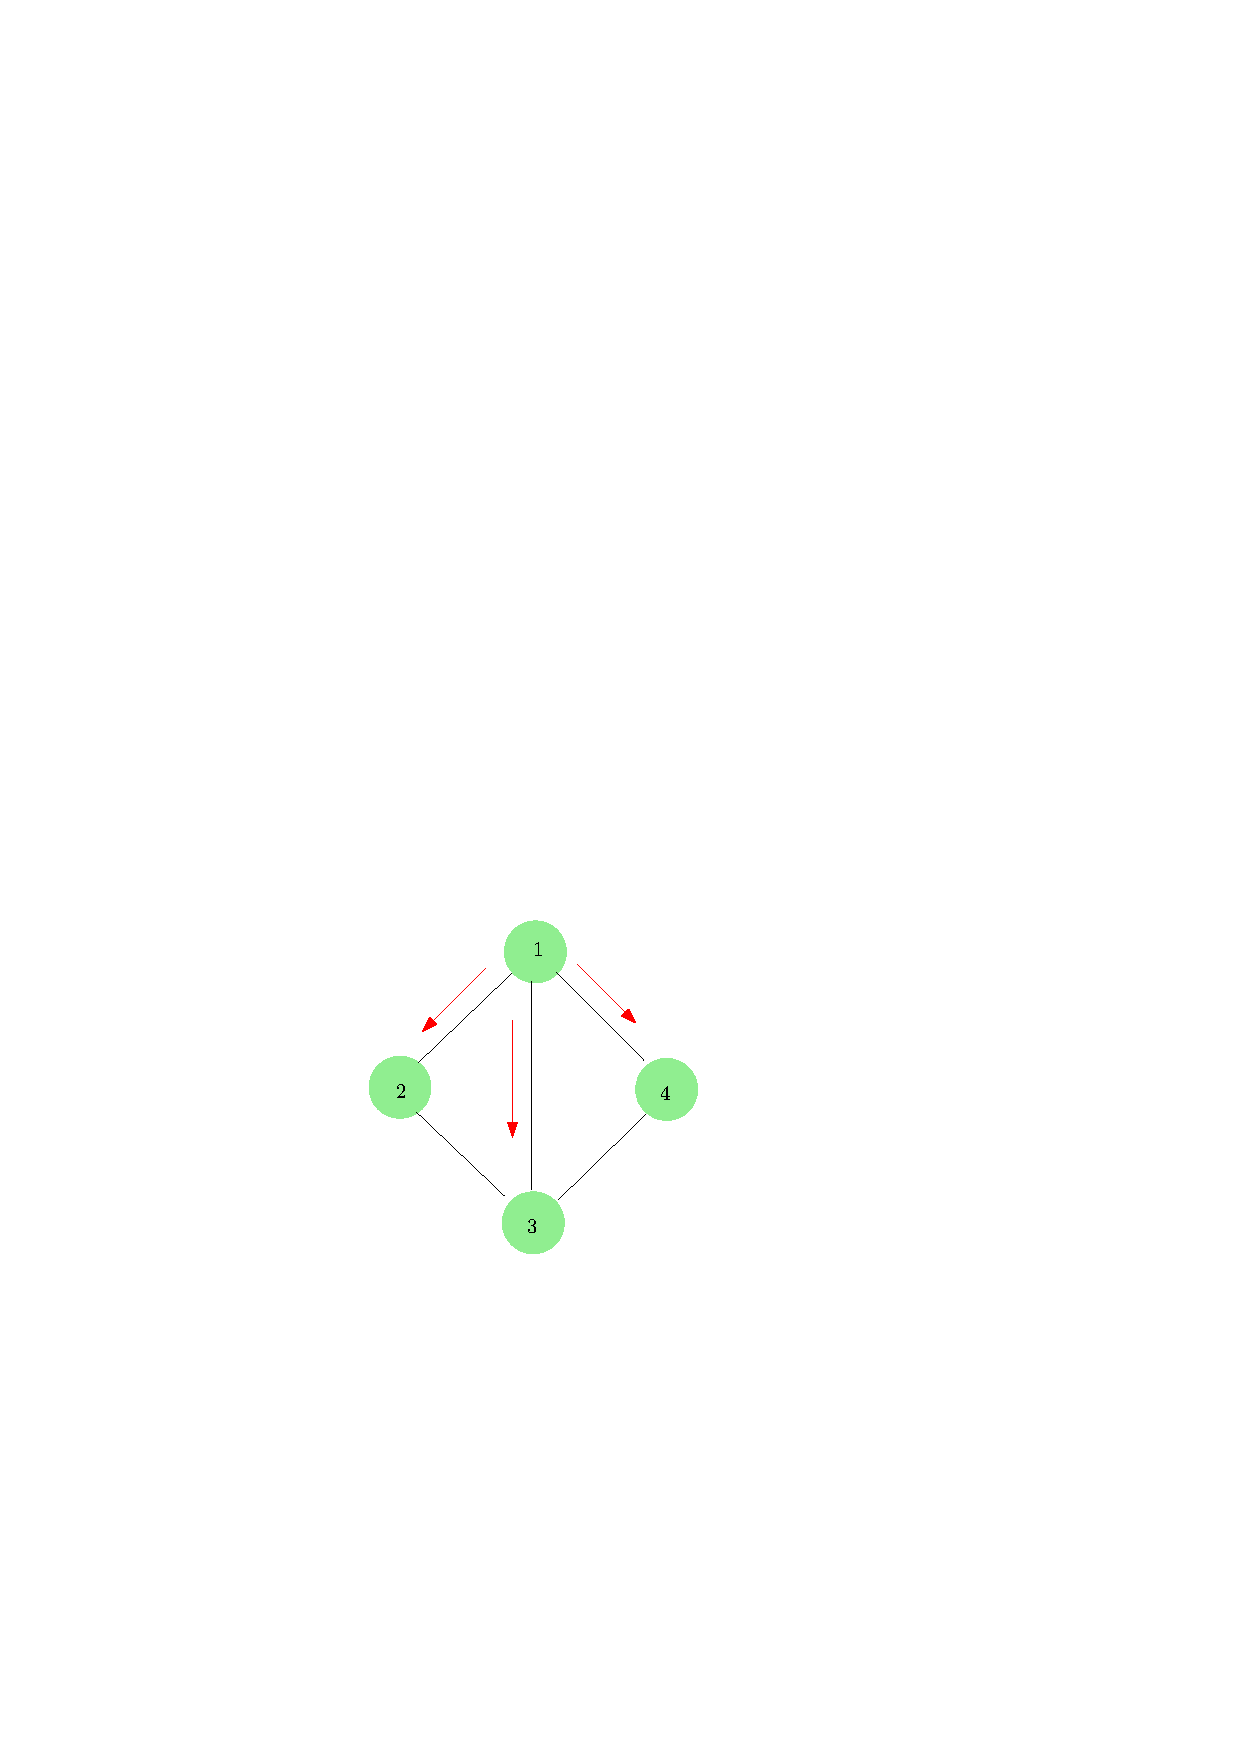
\includegraphics[width=0.32\textwidth]{chapters/background/images/echo/sync/notext_f0_1.pdf}}
    \subcaptionbox{Round Two}{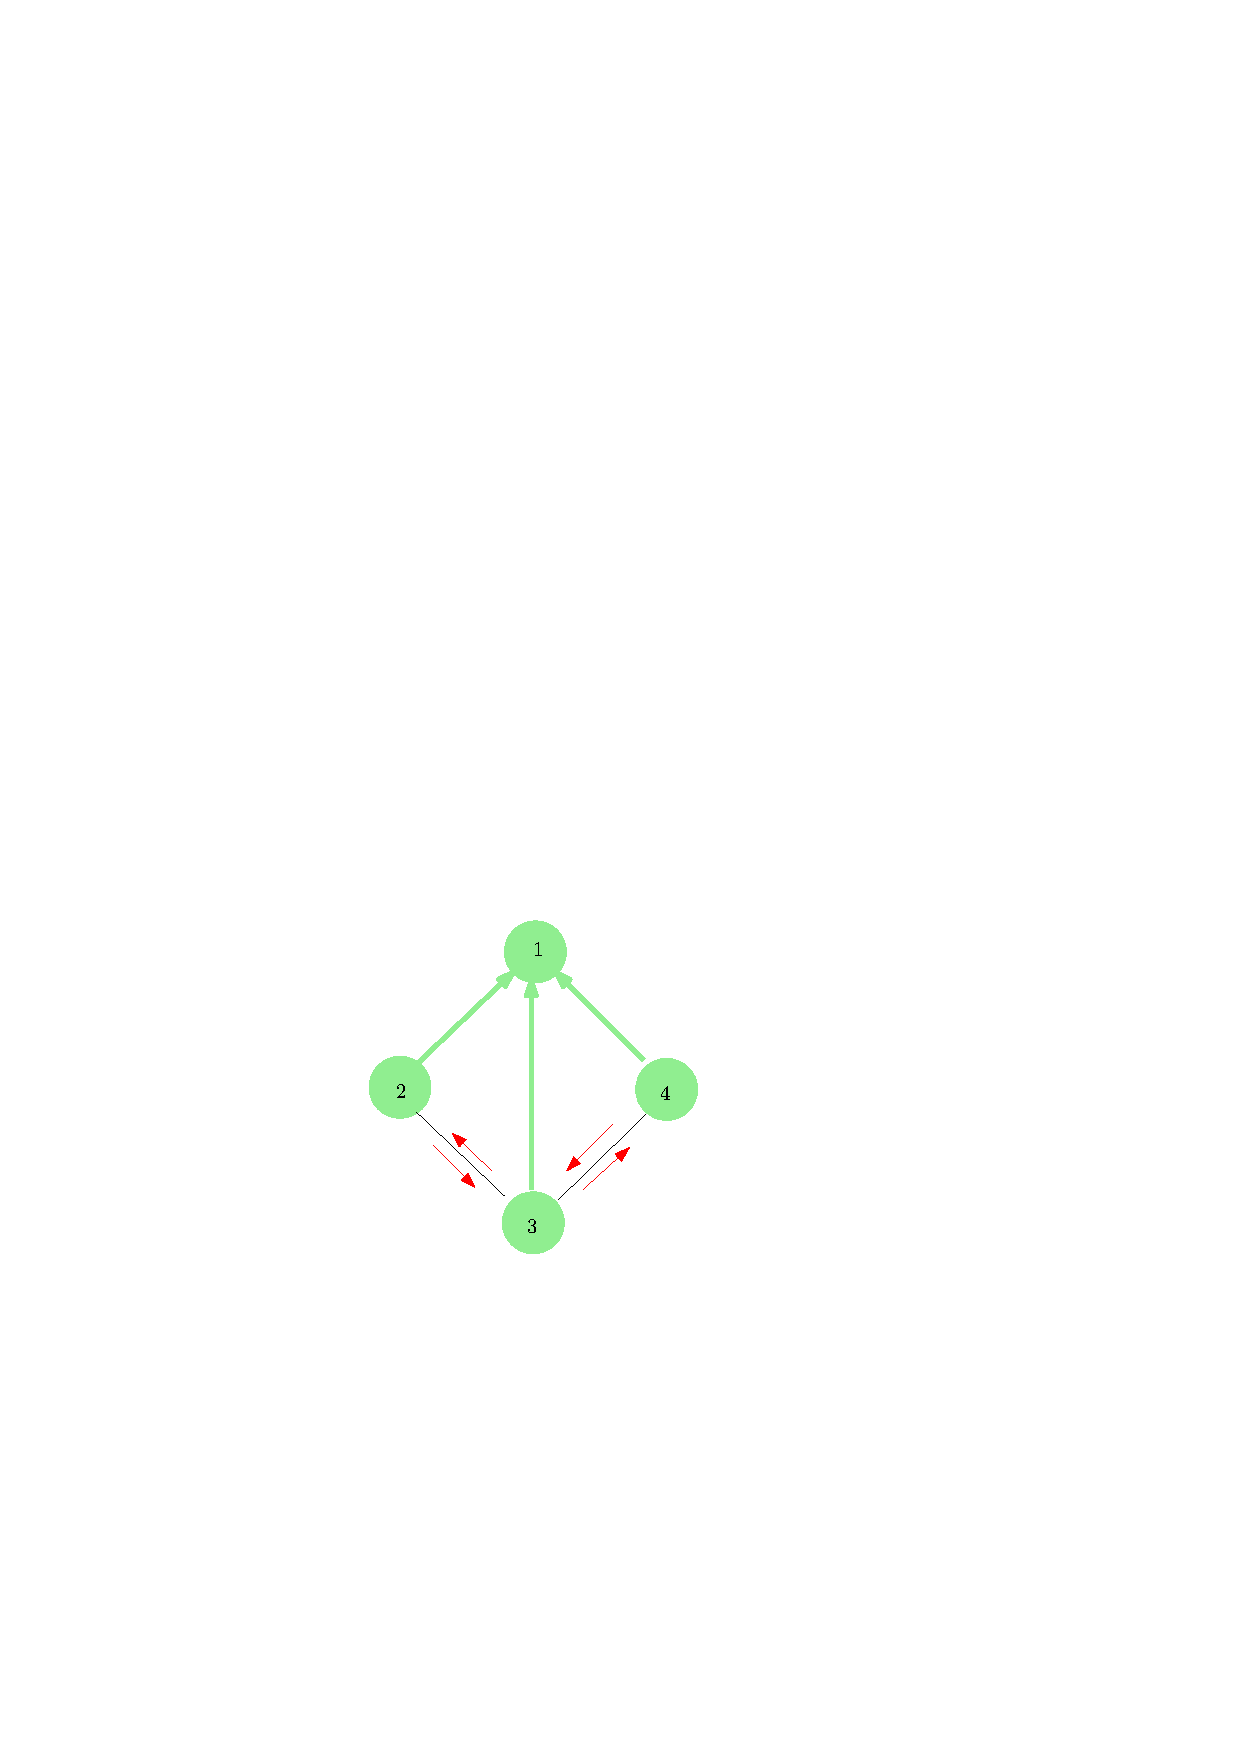
\includegraphics[width=0.32\textwidth]{chapters/background/images/echo/sync/notext_f0_2.pdf}}
    \subcaptionbox{Round Three}{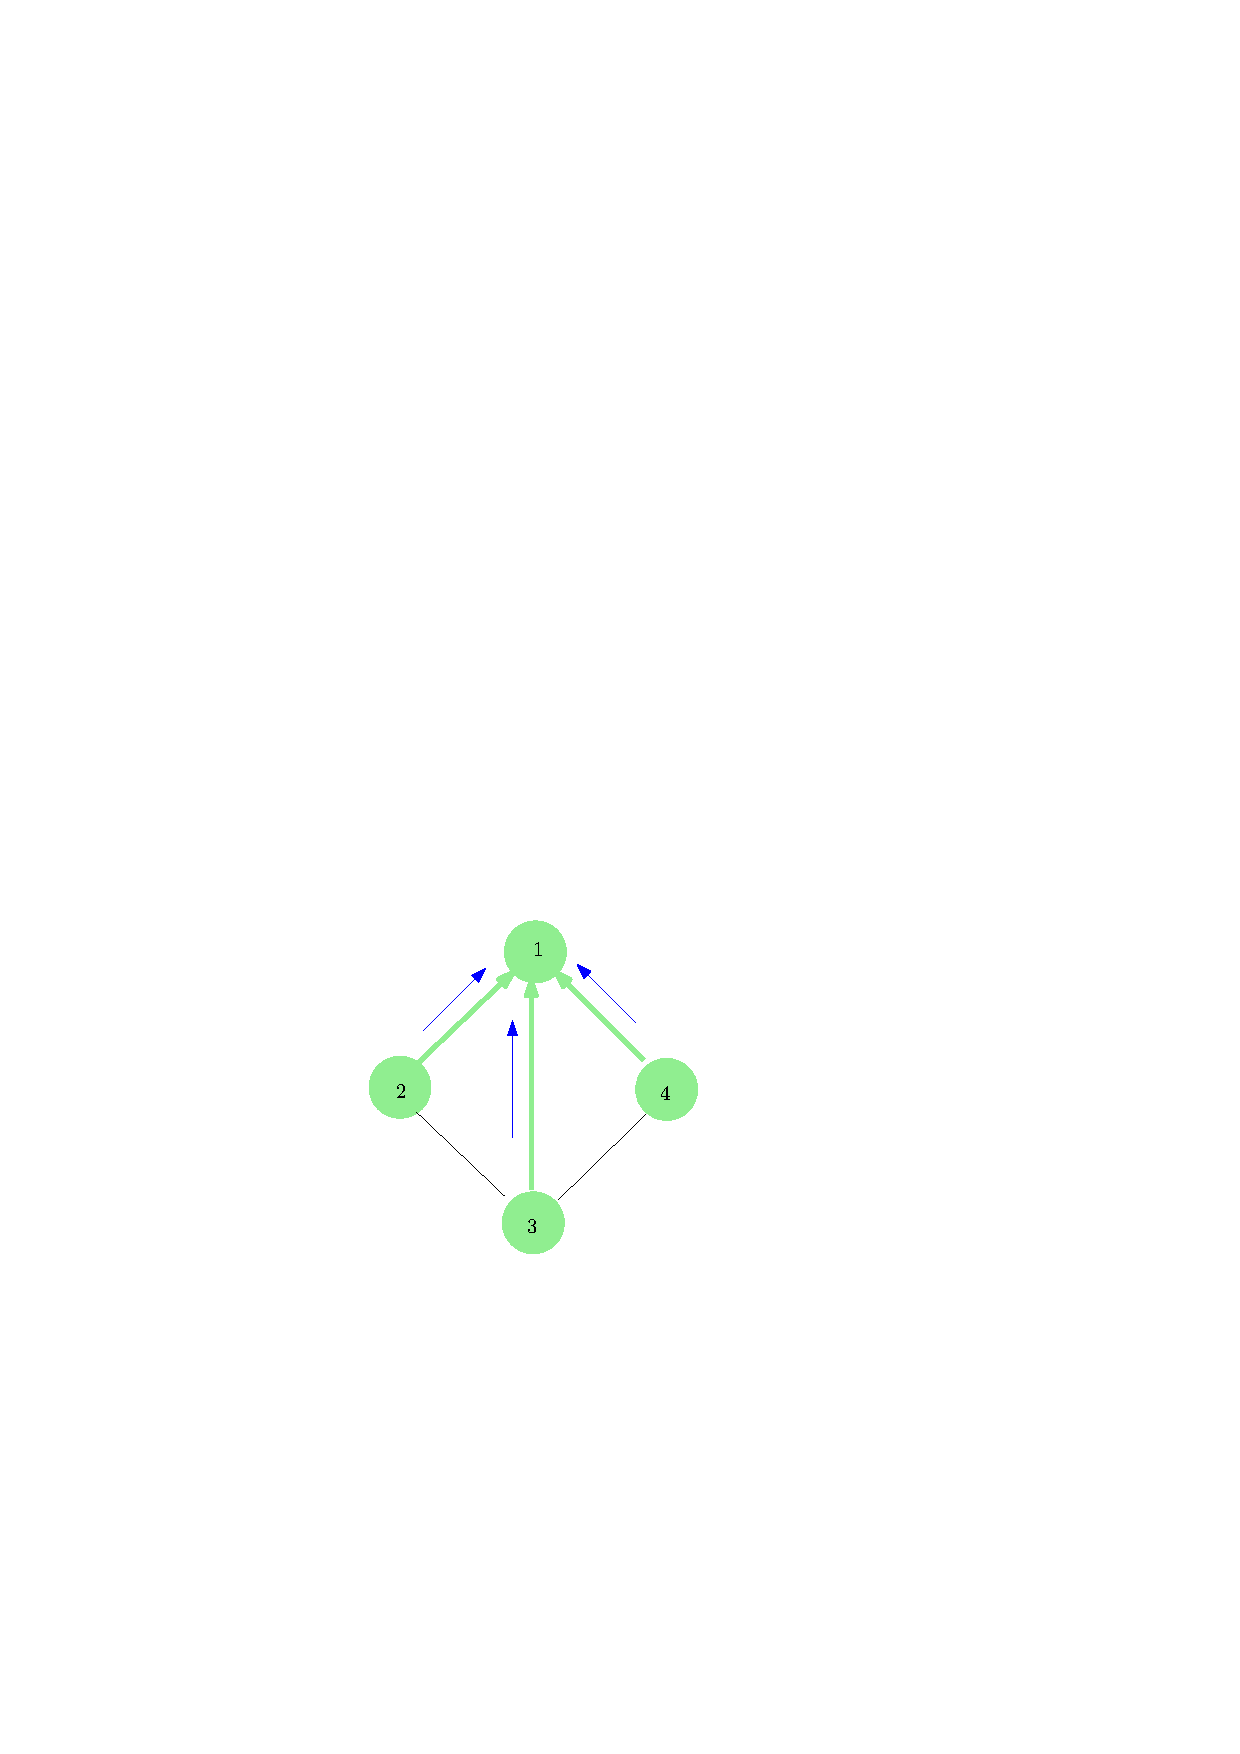
\includegraphics[width=0.32\textwidth]{chapters/background/images/echo/sync/notext_f0_3.pdf}}
    \caption[Progression of the synchronous \textsf{echo} algorithm]{Progression of the synchronous \textsf{echo} algorithm, starting from round zero before any messages are sent.  Arrows in red mean broadcast messages, while arrows in blue mean convergecast messages.}
    \label{fig:back:echosync}
\end{figure}

\begin{figure}[htbp]
    \centering
    \subcaptionbox{Round Zero}{\includegraphics[width=0.32\textwidth]{chapters/background/images/echo/async/notext_f0_0.pdf}}
    \subcaptionbox{Round One}{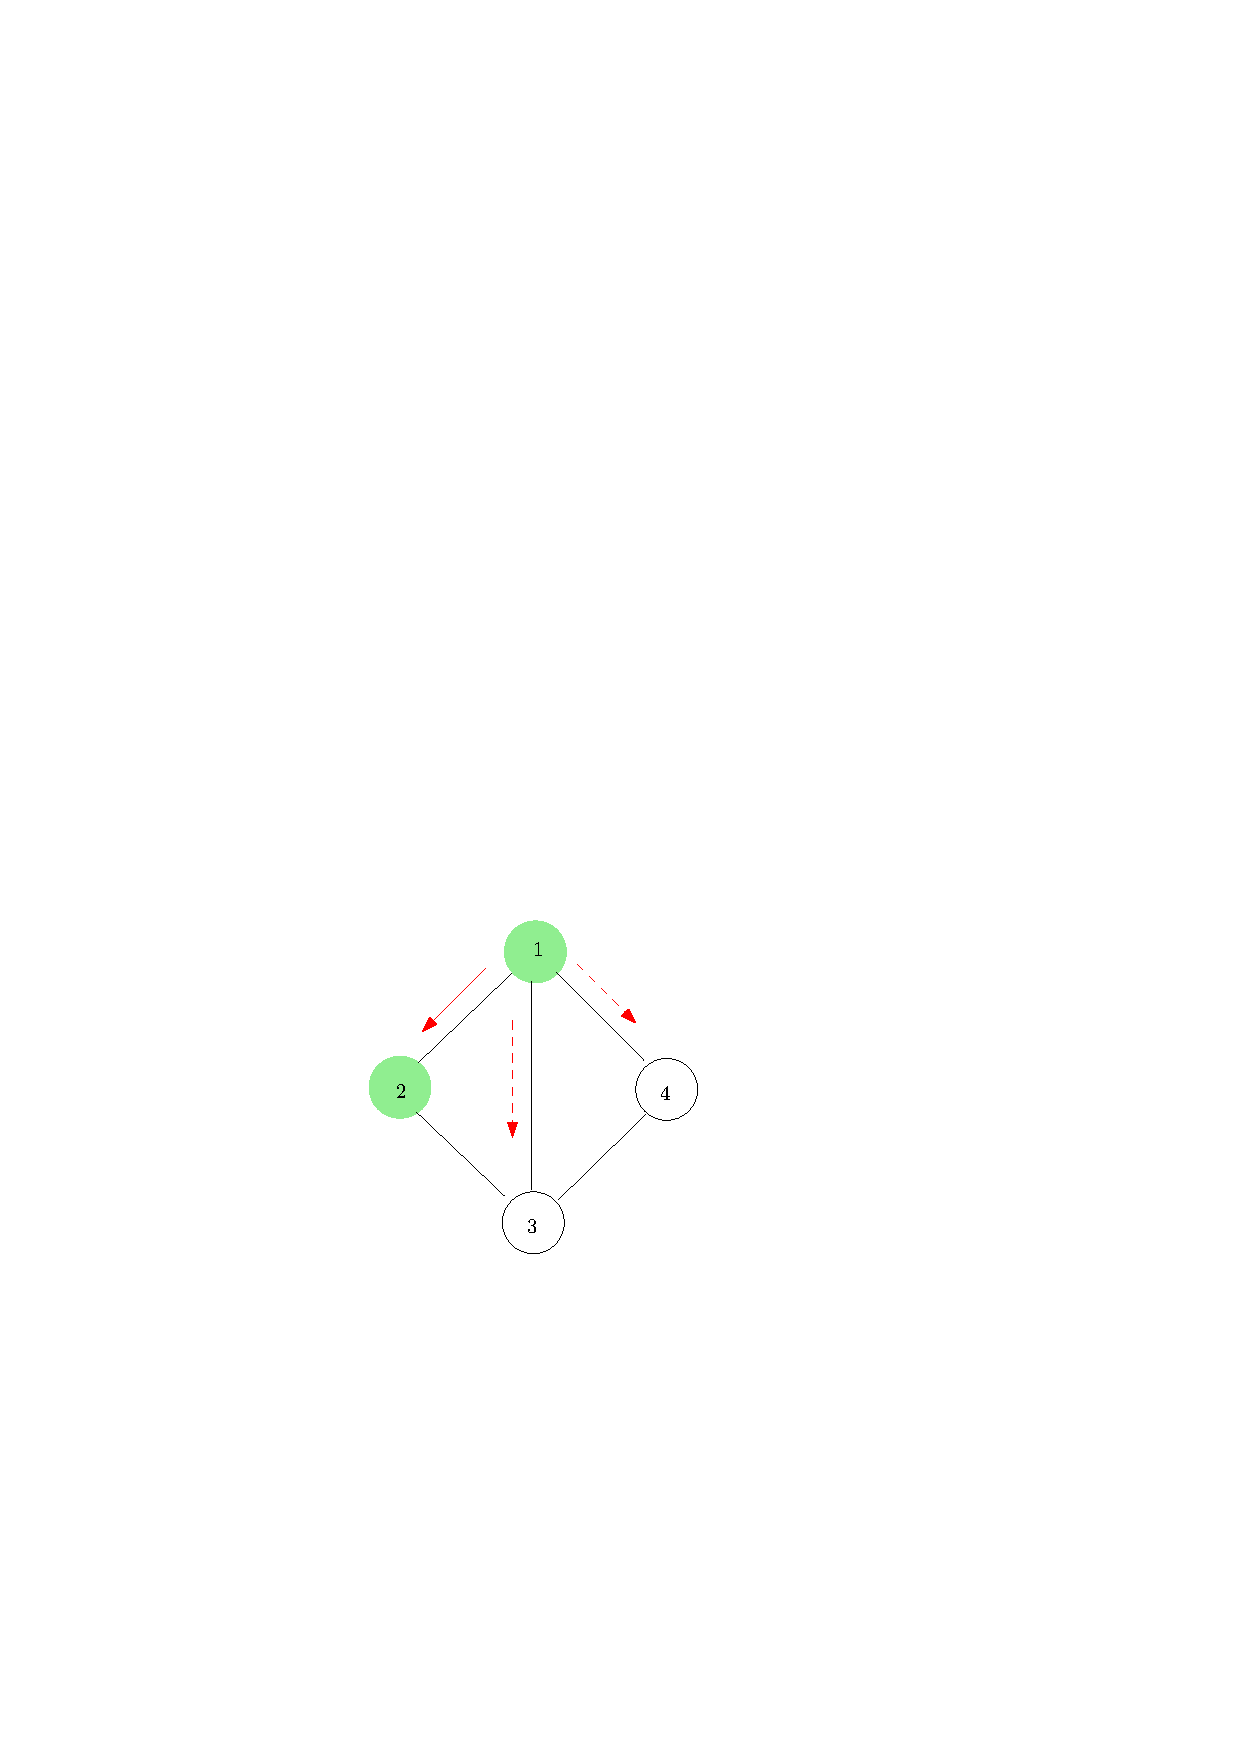
\includegraphics[width=0.32\textwidth]{chapters/background/images/echo/async/notext_f0_1.pdf}}
    \subcaptionbox{Round Two}{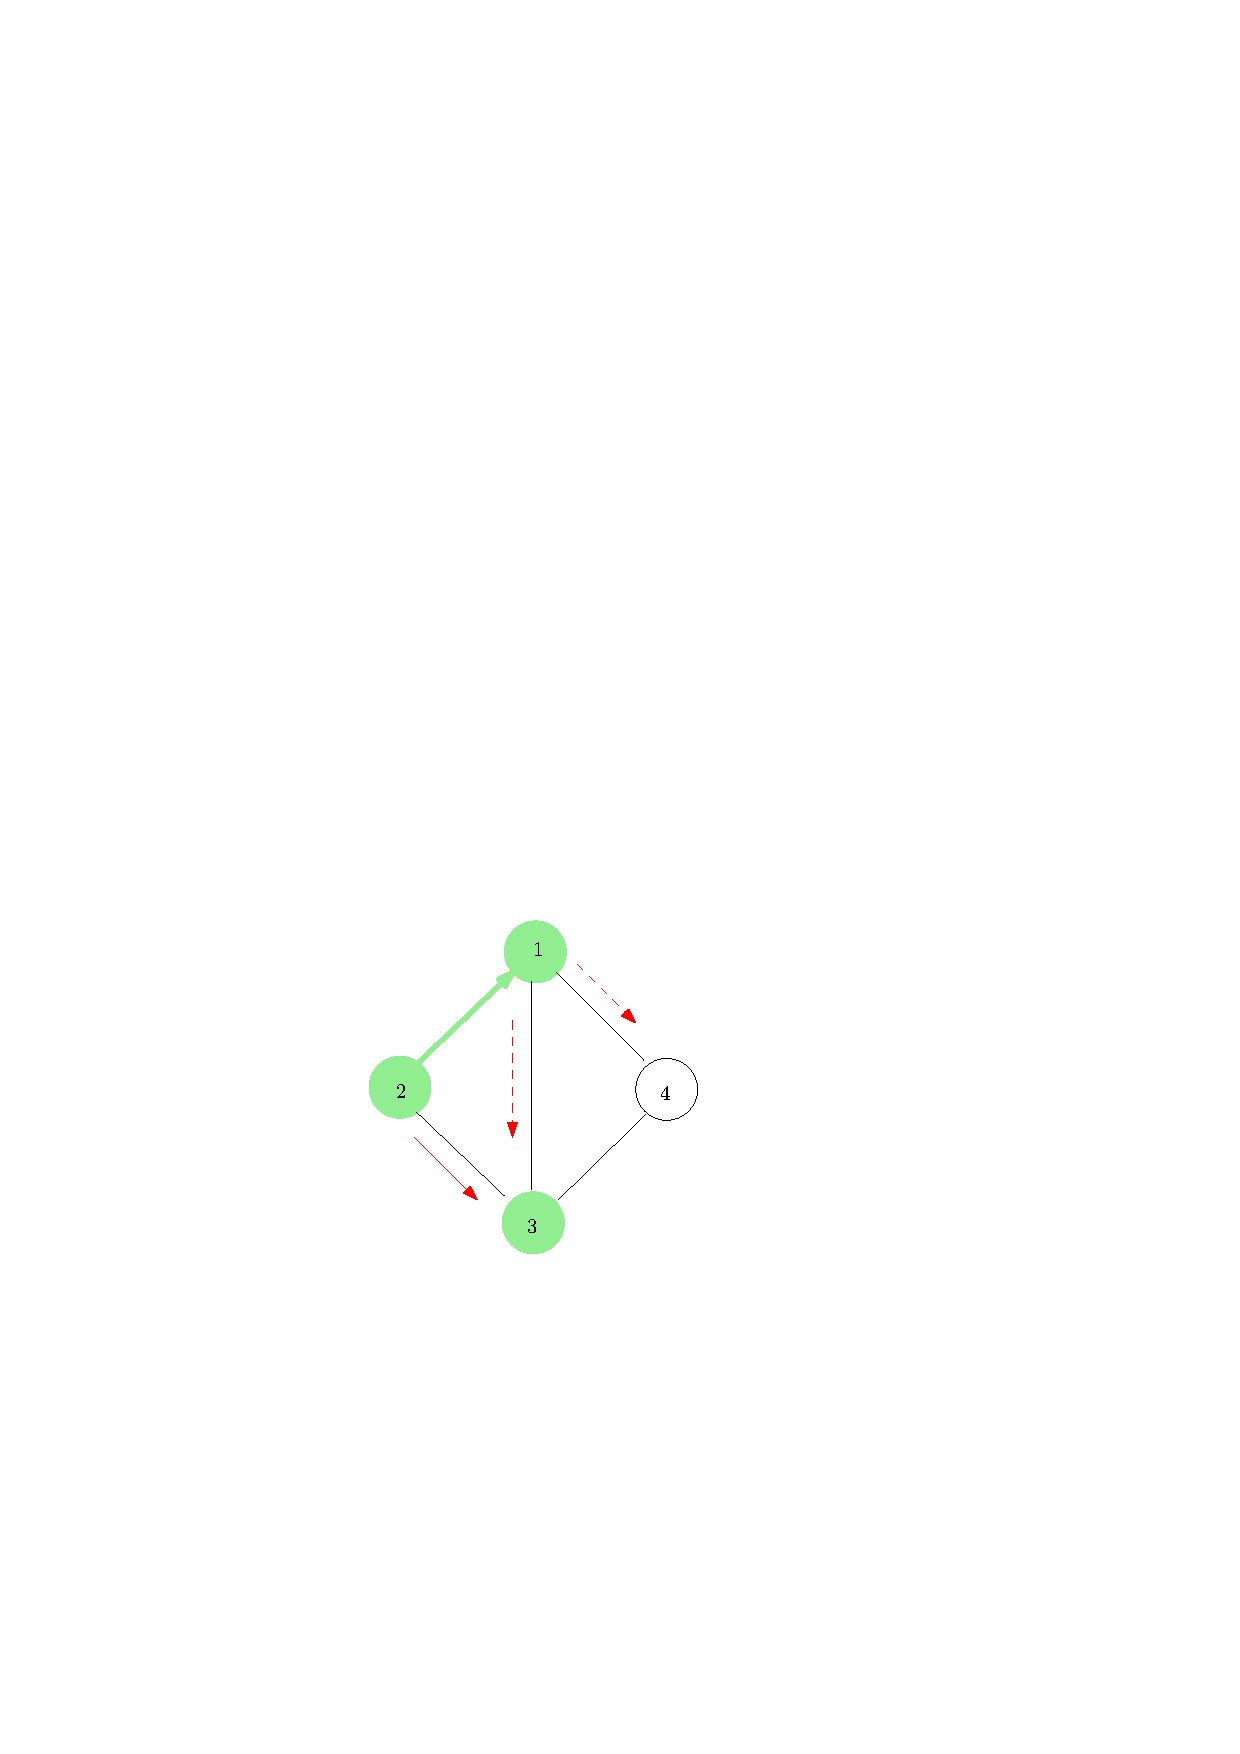
\includegraphics[width=0.32\textwidth]{chapters/background/images/echo/async/notext_f0_2.pdf}}
    \subcaptionbox{Round Three\label{fig:back:echoasync:3}}{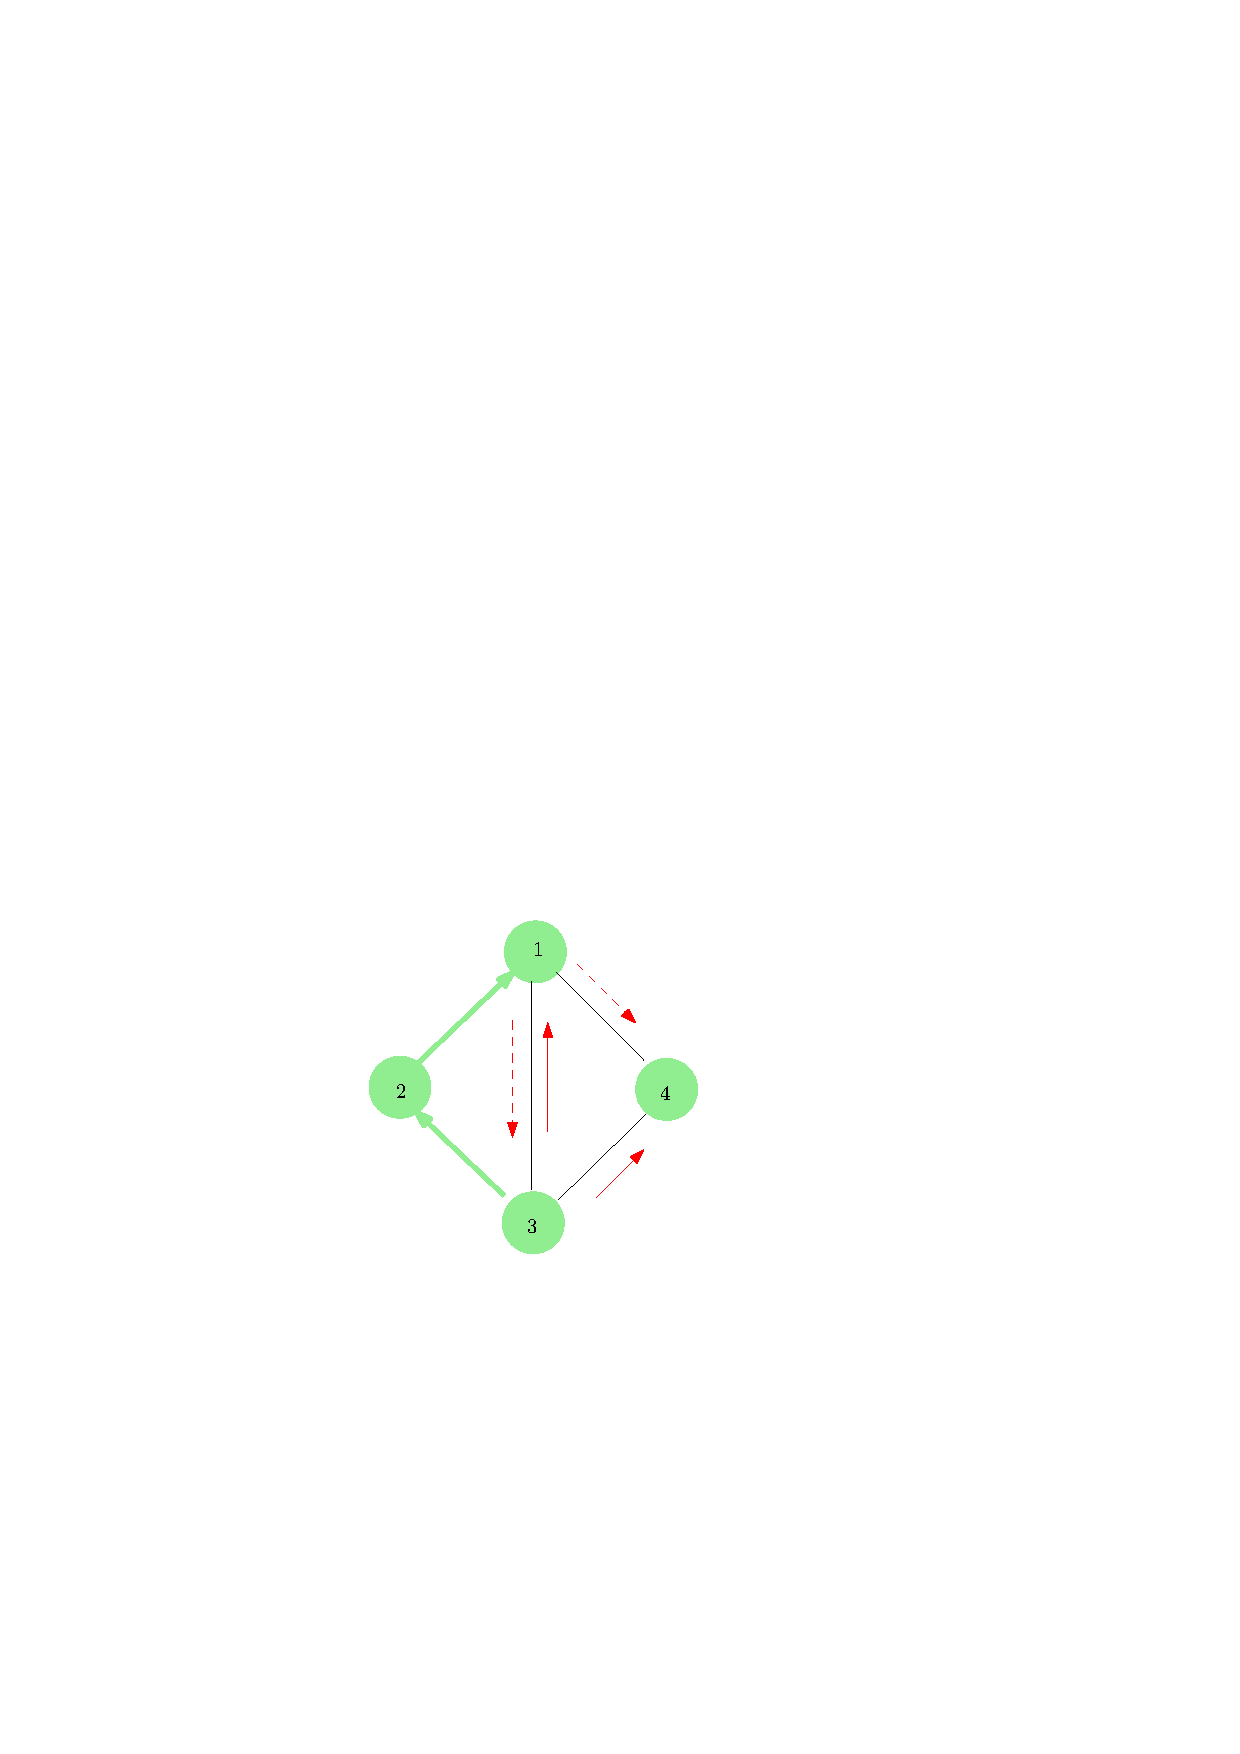
\includegraphics[width=0.32\textwidth]{chapters/background/images/echo/async/notext_f0_3.pdf}}
    \subcaptionbox{Round Four}{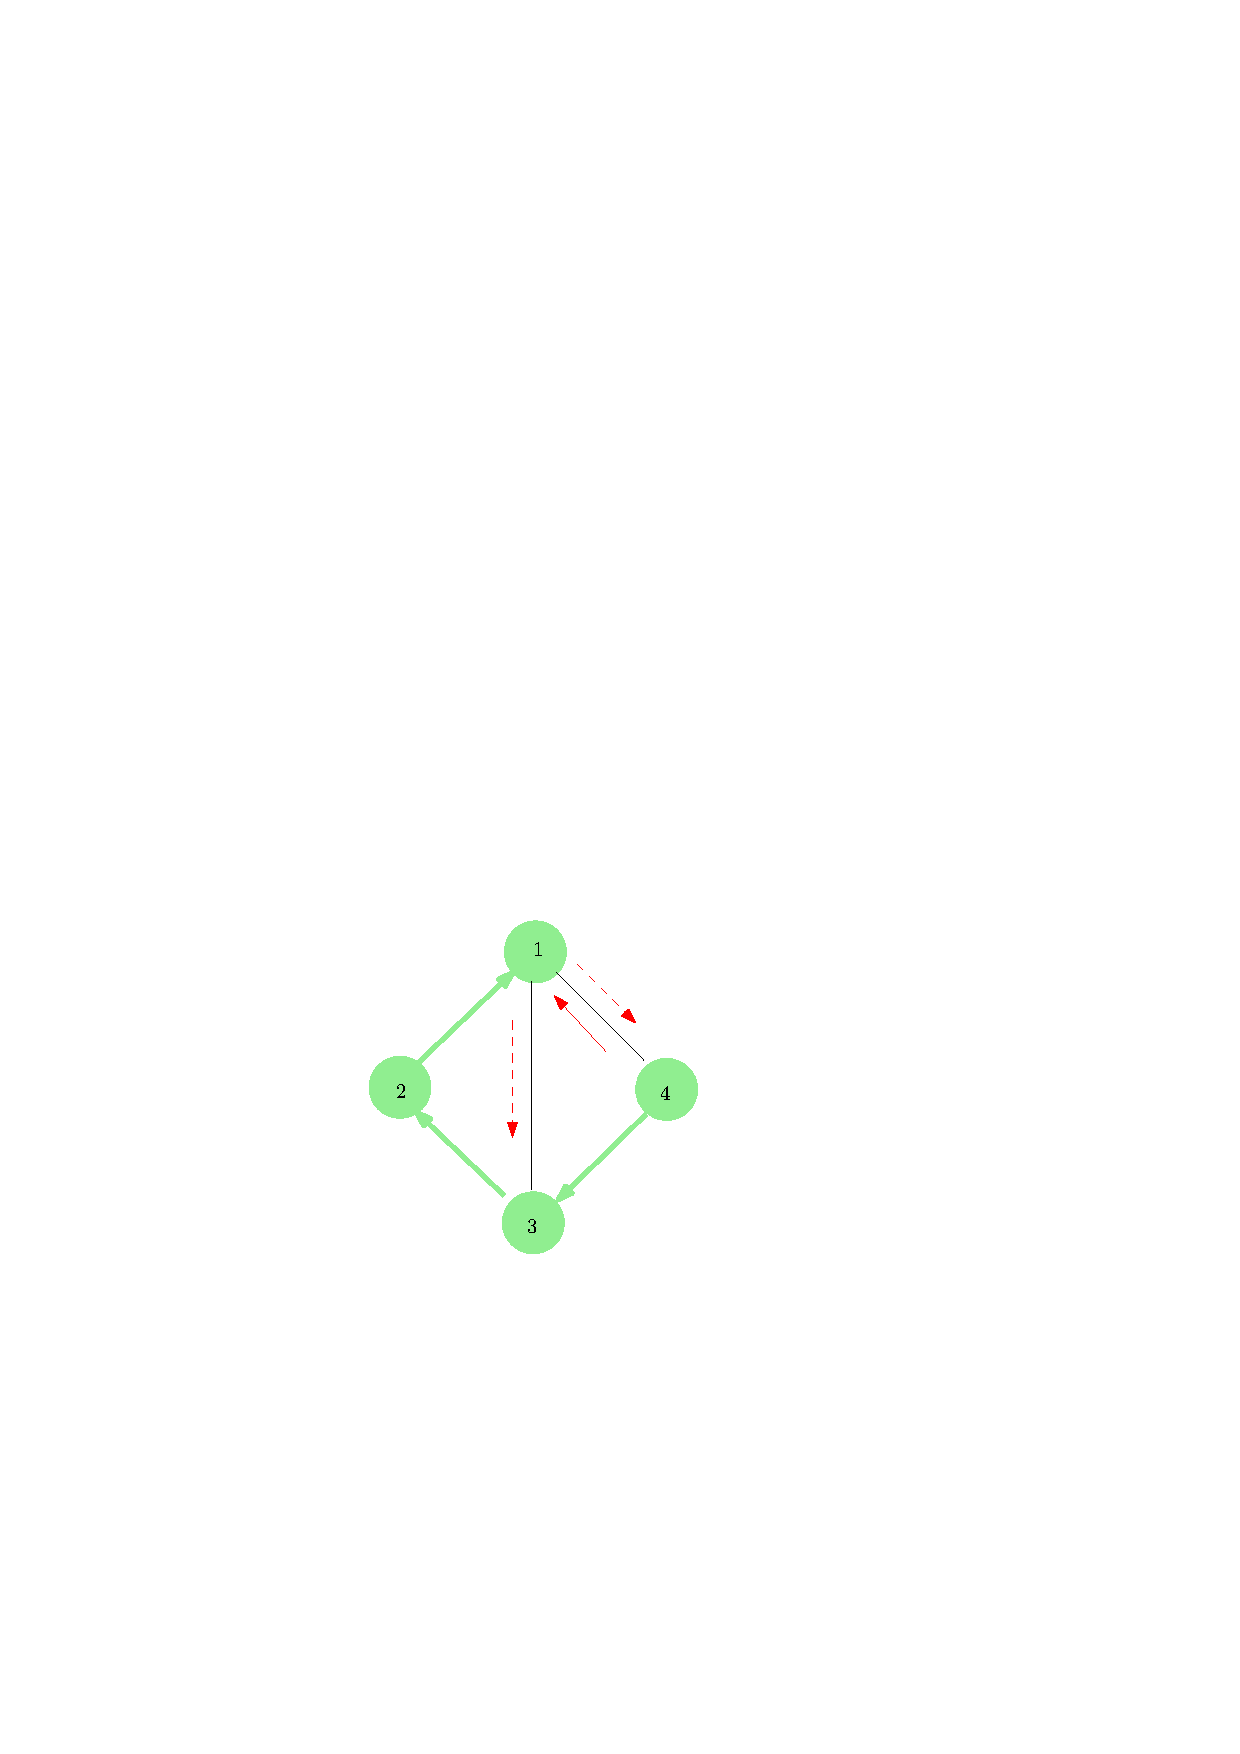
\includegraphics[width=0.32\textwidth]{chapters/background/images/echo/async/notext_f0_4.pdf}}
    \subcaptionbox{Round Five}{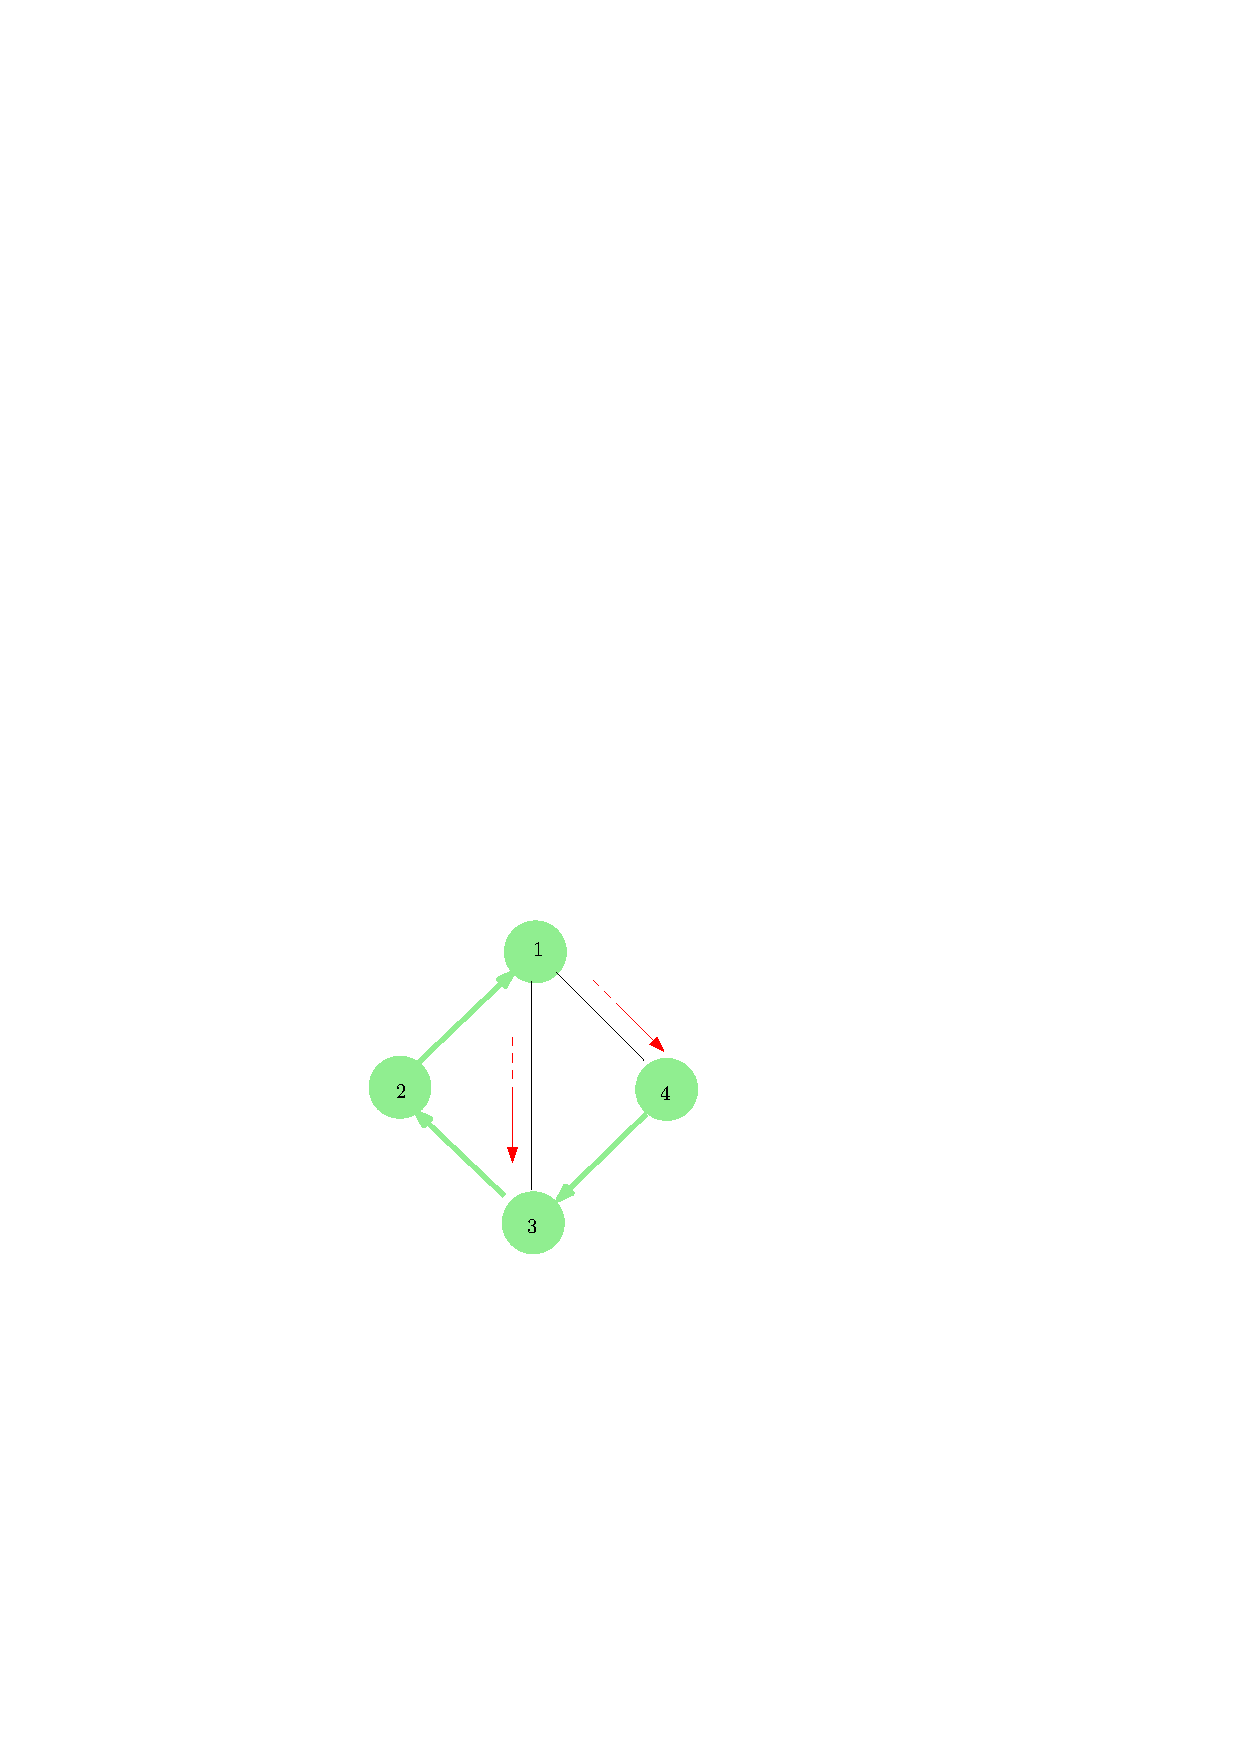
\includegraphics[width=0.32\textwidth]{chapters/background/images/echo/async/notext_f0_5.pdf}}
    \subcaptionbox{Round Six}{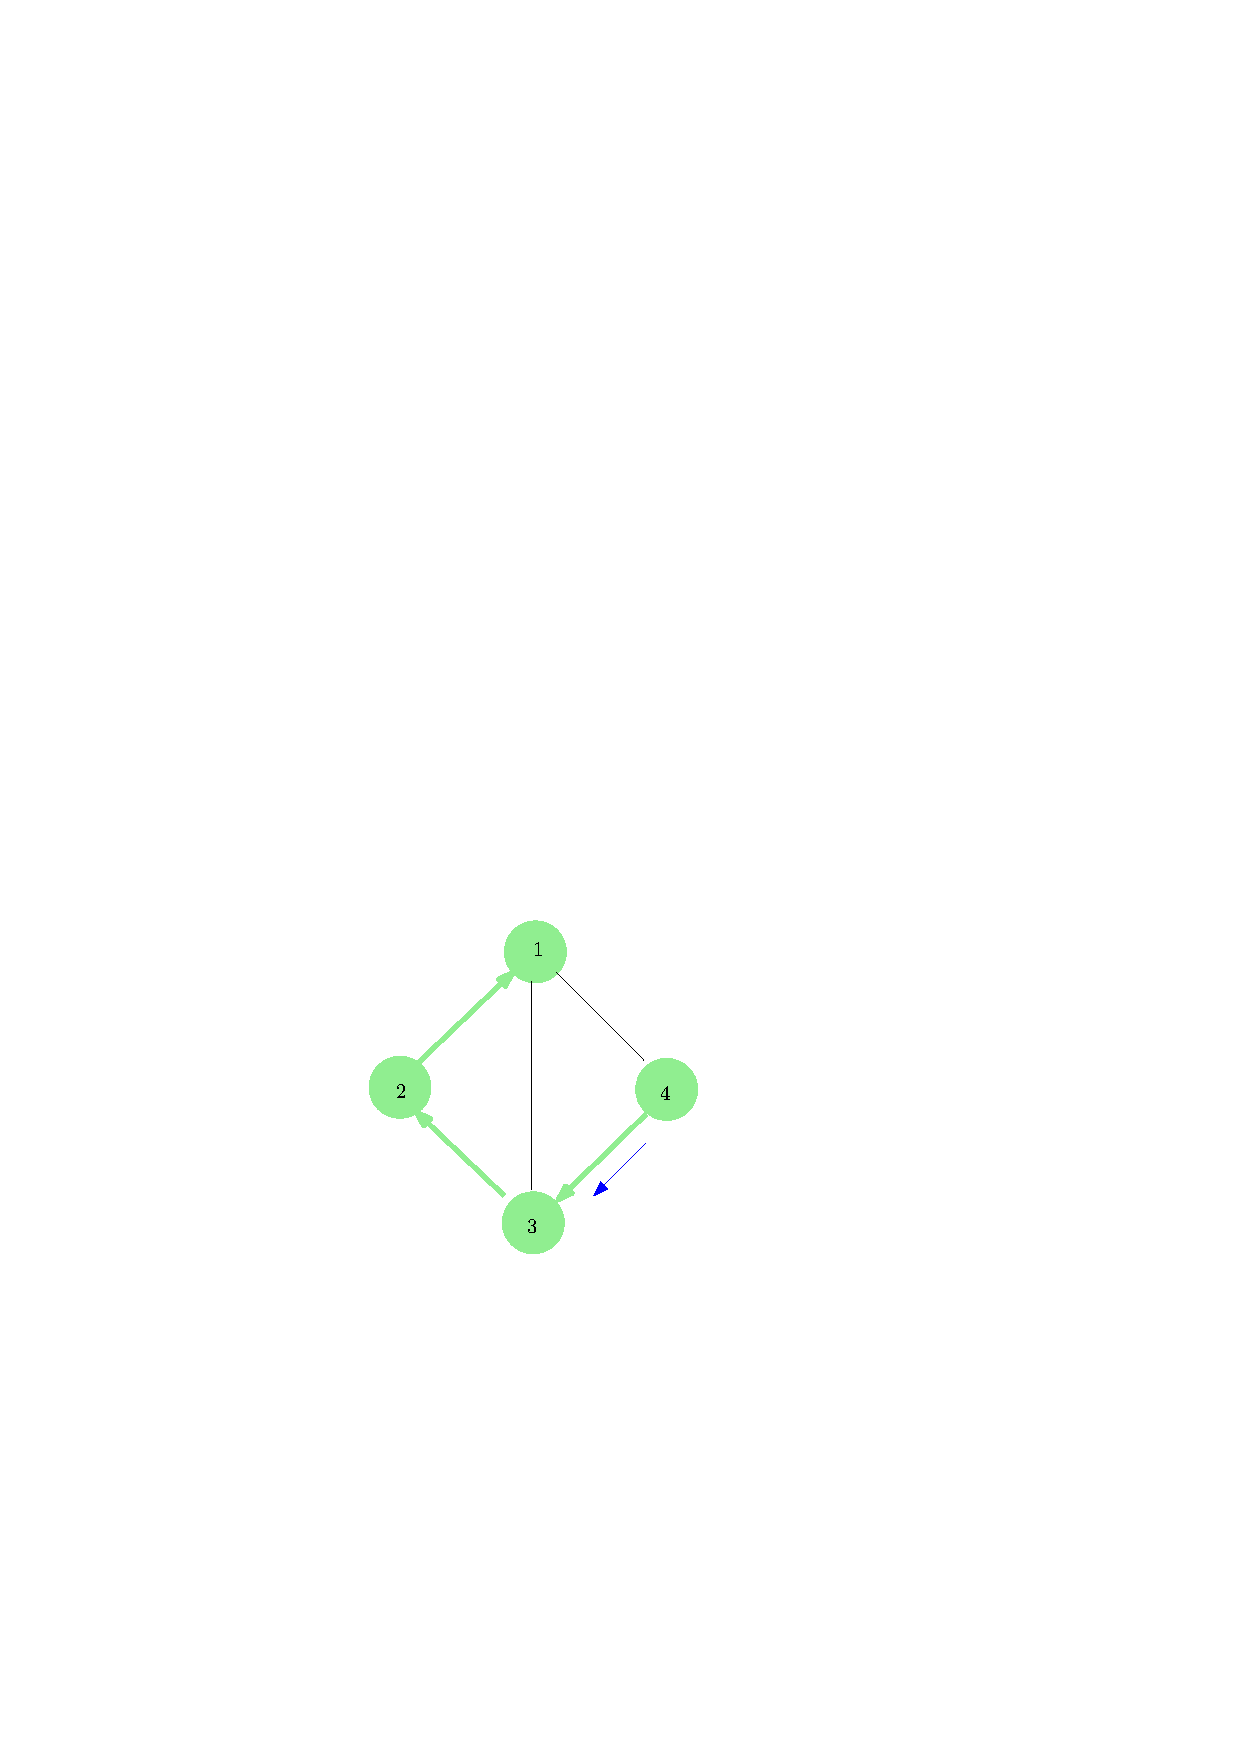
\includegraphics[width=0.32\textwidth]{chapters/background/images/echo/async/notext_f0_6.pdf}}
    \subcaptionbox{Round Seven}{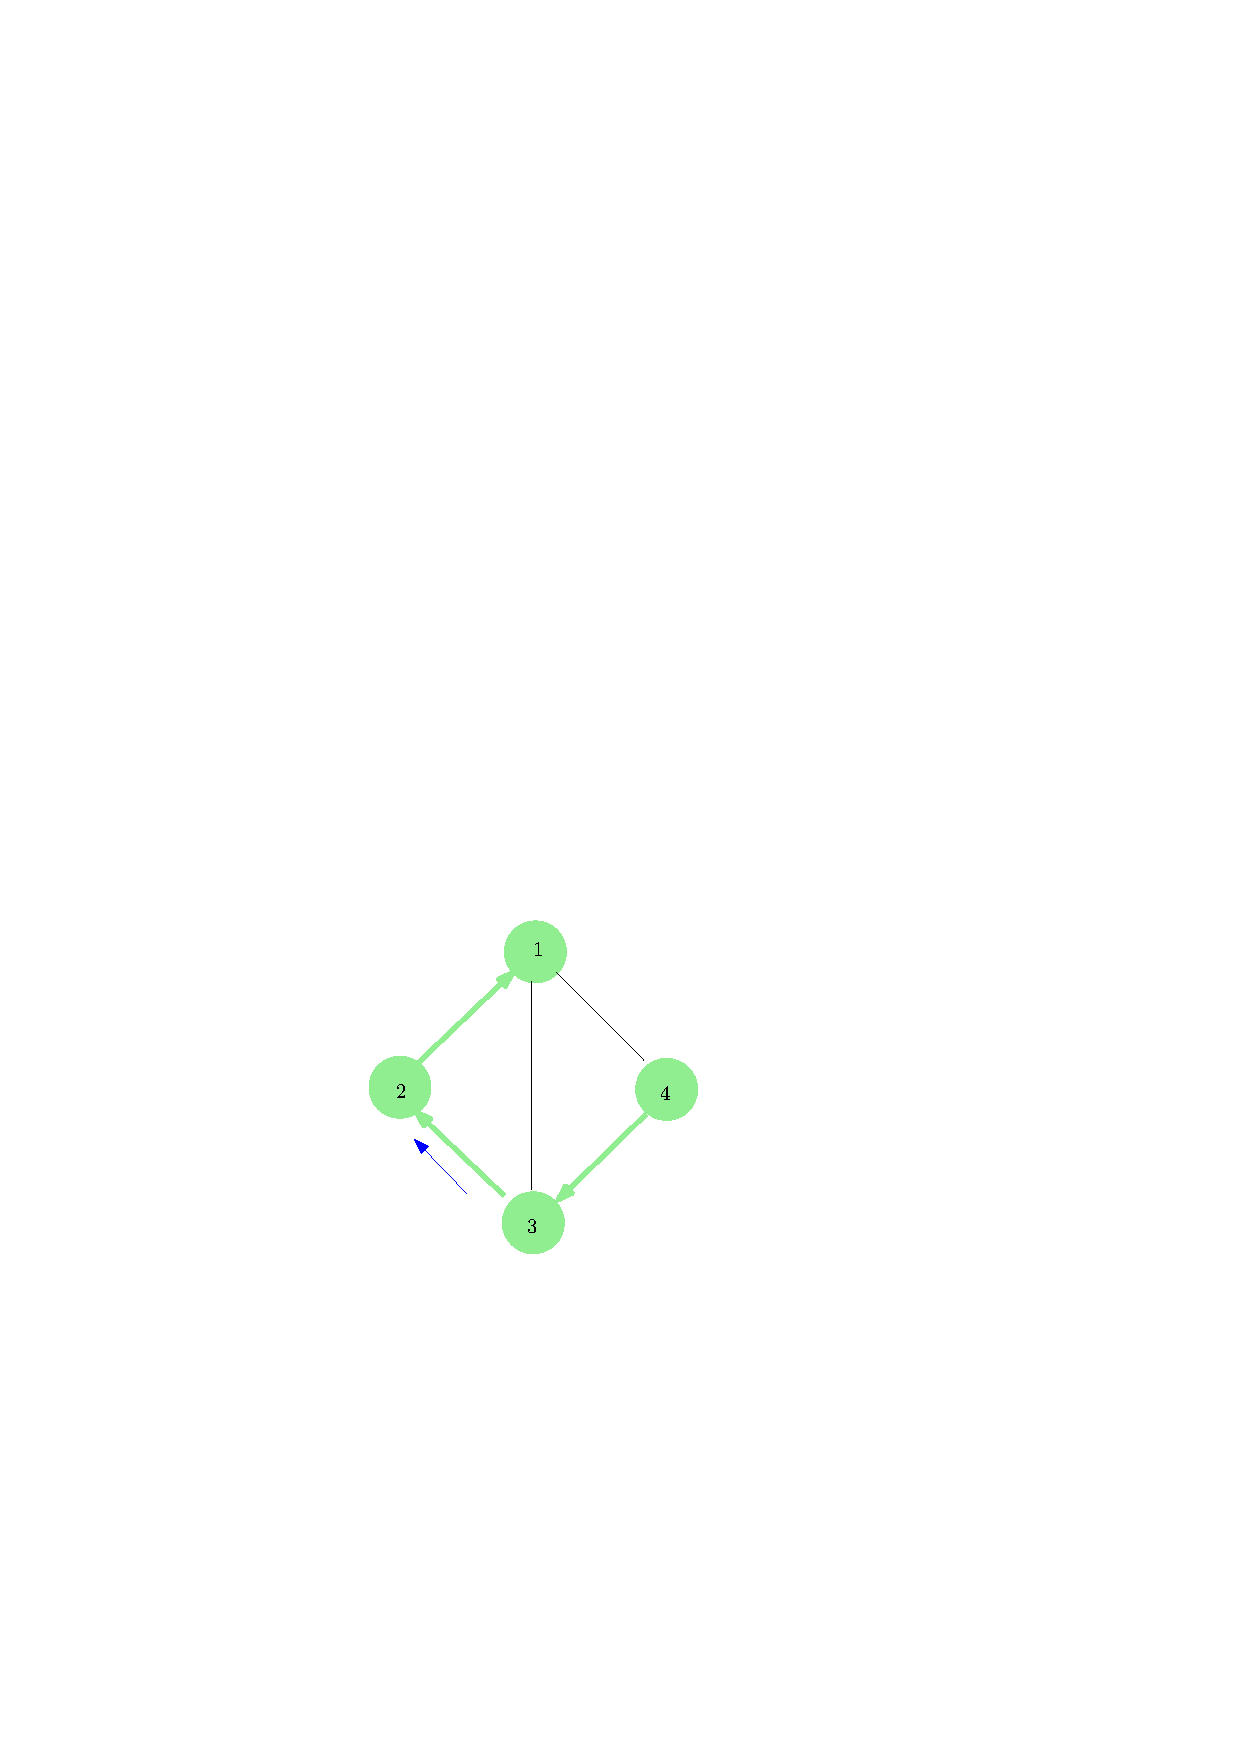
\includegraphics[width=0.32\textwidth]{chapters/background/images/echo/async/notext_f0_7.pdf}}
    \subcaptionbox{Round Eight}{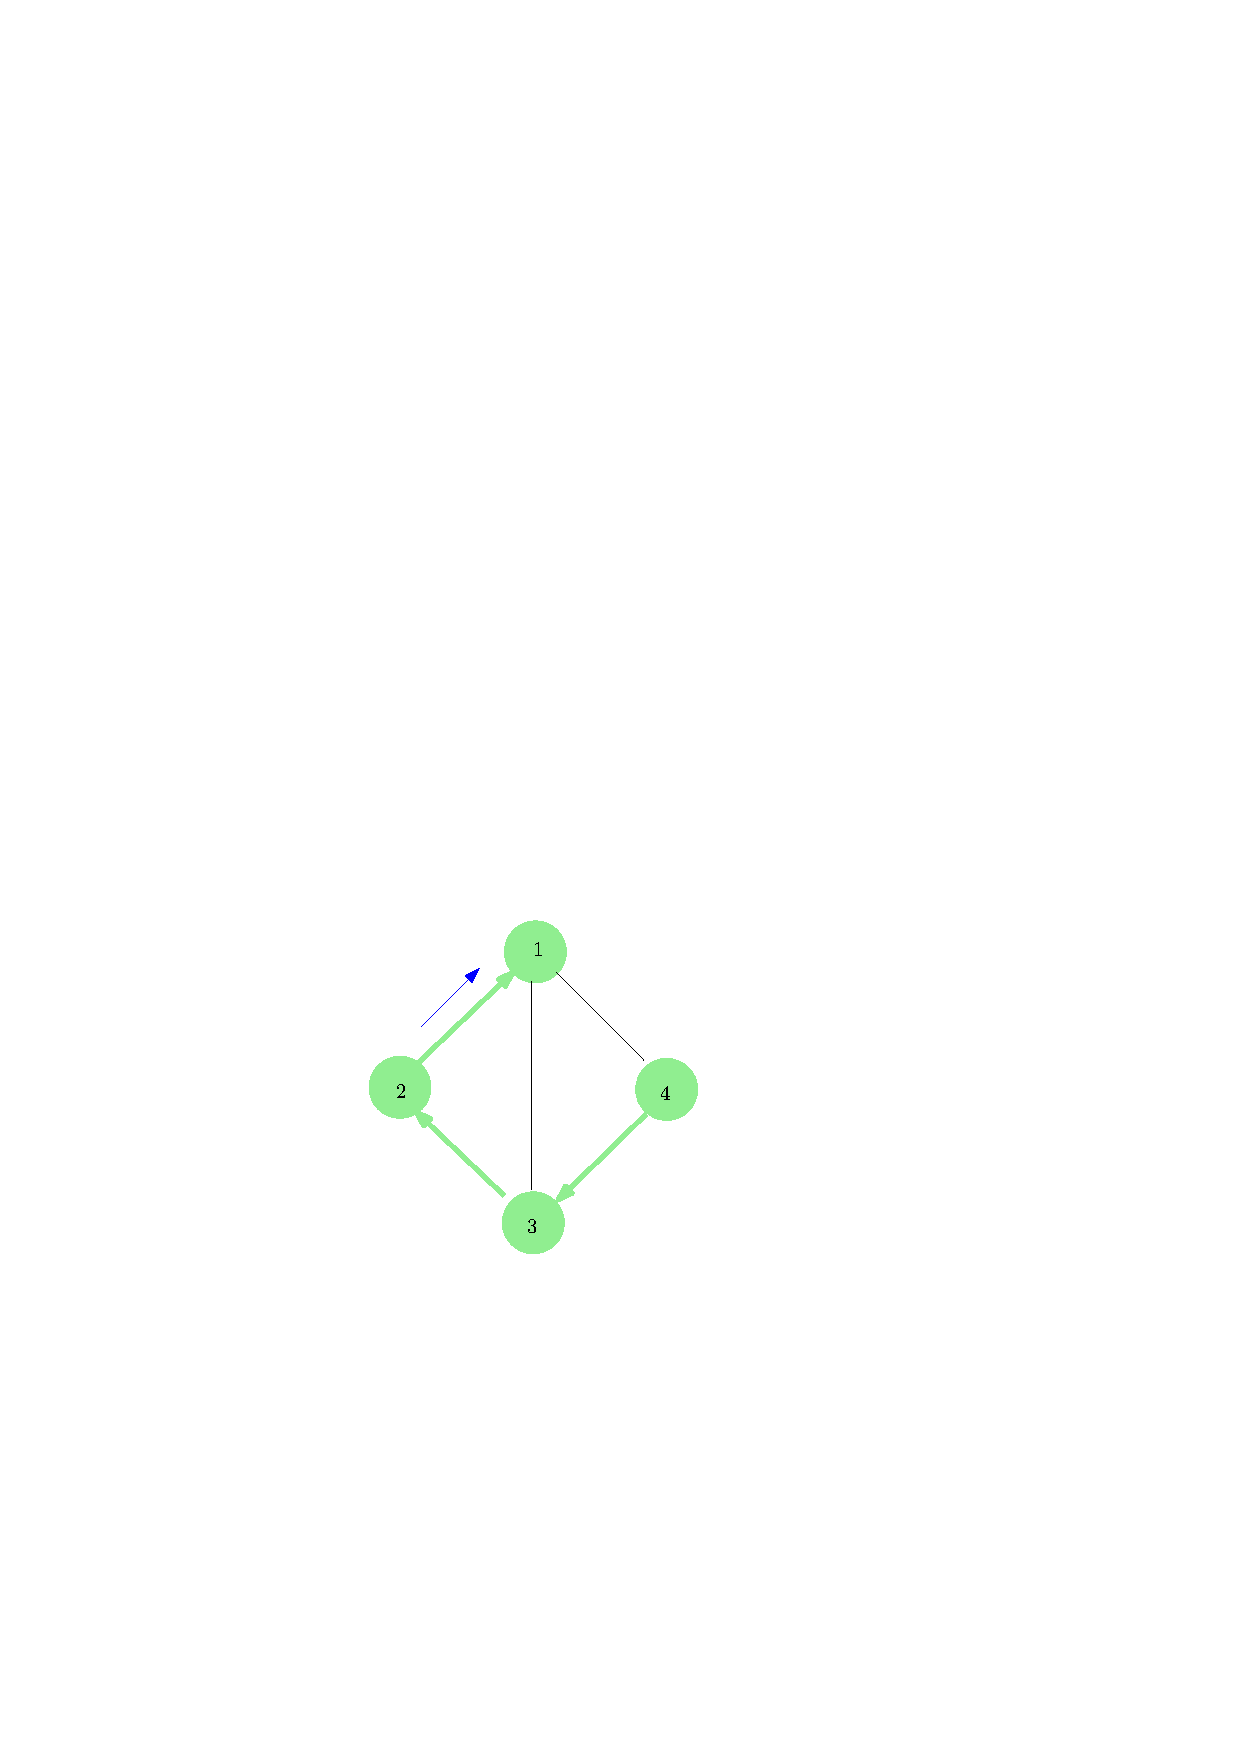
\includegraphics[width=0.32\textwidth]{chapters/background/images/echo/async/notext_f0_8.pdf}}
    \caption[Progression of the asynchronous \textsf{echo} algorithm]{Progression of the asynchronous \textsf{echo} algorithm, starting from round zero before any messages are sent.  Arrows in red mean broadcast messages, while arrows in blue mean convergecast messages.  Despite node 1 being the initiator node, node 4 considers node 3 to be its parent because it first receives a broadcast message from node 3.}
    \label{fig:back:echoasync}
\end{figure}

In the synchronous case, all messages sent out are received simultaneously, and all nodes proceed through their rounds together.  In the asynchronous case, however, messages may arrive at arbitrary times, and nodes proceed through their rounds entirely independently of one another.  The round numbers in the figure mark the point where at least one message has been received by a node.  The nodes react to messages as they arrive, and might do nothing for a time while other nodes are working if no new messages arrive during that time.  Under the asynchronous model, depending on communications topology and speeds, it is possible for the first broadcast message to reach a process to have followed a less direct route from the initiator than otherwise might be possible.  Exactly this is seen in \cref{fig:back:echoasync:3}, where node 4 first receives a message from node 3 (and thus marks node 3 as its parent), despite a direct connection to the initiator, node 1.
\section{\label{sec:back:cml}\glsfmtlong{cml-glossary}}

While parallelism is often the best (perhaps only) way to achieve improvements in execution time for different algorithms once an efficient sequential implementation has been created, it is a notoriously challenging affair \cite{Shun2017}.  When working at the level of directly manipulating threads, such as using the pthreads found in POSIX-compliant operating systems, programmers are exposed to a high level of risk of inadvertently introducing concurrency bugs, such as data races, deadlocks and livelocks.  A panoply of approaches to overcoming this challenge, both theoretical and practical, have been proposed and developed over the years, with varying degrees of success, \eg{} \cite{Boyapati2002,Bocq2012,Seinstra2004}.  Many, perhaps most, large-scale programming languages that use a runtime include some form of parallelism simplification within their standard libraries, \eg{} the Executor system in Java \cite[Ch. 4]{Fernandez2012}, and Swift \& Objective-C's Grand Central Dispatch \cite{Maskrey2018}.

Most simplifications fairly directly target either data-parallelism by simultaneously applying the same operation over multiple elements in arrays, \eg{} SIMD instructions in CPUs \cite{Hughes2015}; or task-parallelism by making provisions for the fork-join model \cite{McCool2012}.  These simplifications can be very useful, but not all instances of parallelism fit neatly into their models.  Algorithms that are well-modelled by the \Gls{csp} and \Gls{actor} models, such as those explicitly centred around concepts of message passing, are not necessarily easy to express using either SIMD or fork-join instructions.

\Gls{cml} \cite{Reppy1991,Panangaden1997} is an approach to concurrent programming originally developed by John Reppy (based on his earlier `Pegasus Meta-Language' \cite{Reppy1988}).  \Gls{cml} was created to provide a framework for creating concurrent programs with synchronous communications on single-core machines,\footnote{In fact, the original implementation \emph{relied} on the fact that the processor was single-core under-the-covers.} and was later extended to permit parallelism \cite{Reppy2009a}.  It was created originally as a library in Standard ML of New Jersey (where ML refers to the earlier programming language \textit{Meta Language}), whence the ML part of the name, but its concepts have subsequently appeared elsewhere.  The basic concept of communicating via channels has experienced a renaissance in recent years, likely due at least in part to its inclusion as a core feature of Go \cite{Meyerson2014}, but \gls{cml} has a more advanced system that Go (at the time of writing) does not fully support.

\Gls{cml} is designed to avoid many of the problems with concurrency that arise in traditional sequential programming, where the use of locks, mutexes and semaphores etc. are frequently required, and often lead to the potential introduction of problems such live-/deadlocks, data races and extreme resource contention.  This is achieved by changing the approach to concurrent programming to one of logically separate, internally sequential processing elements that share data as required by `passing messages'\footnote{This is the logical concept, but there is not strictly any specific required software implementation.} between themselves.  In \gls{cml}, these logical processing elements are referred to as threads, and they exchange messages over channels \emph{synchronously} (called \emph{rendezvous}), \ie{} there is a temporal overlap between one thread offering to send, and another to receive, over the same channel, and the first to offer blocks until the second makes its offer.  When two processes are offering appropriately on either side of an exchange, rendezvous takes place.

Reppy describes a concurrent program as one that supports multiple sequential sub-programs conceptually executing in parallel separately, but interacting through shared resources to achieve a common goal.  \Gls{cml} is concerned with the scenario where said interactions are explicit, and in order to facilitate that \enquote{\gls{cml} takes the unique approach of supporting \emph{higher-order concurrent programming}} (emphasis Reppy's), whereby communication and synchronisation are made into first-class members of the language, similar to how functional programming languages made functions into first-class members of themselves \cite[Preface]{Reppy2007}.

\begin{anfxerror}{Expand this?}
Describe more of how \gls{cml} works?  Is there not something in the gcol chapter that can be shifted into here, at least?
\end{anfxerror}
\section{\label{sec:back:mc}\Glsfmtname{mc}/\glsfmtname{ps}}

\emph{\Gls{mc}}, also known as \emph{\gls{ps}} (the two terms are generally used interchangeably), is a bio-inspired model of computing created by Gheorghe Păun in the late 1990s \cite{tPaun98a,Paun2000}.  It was originally conceived of by considering the process of chemical reactions and exchanges that occur inside living biological cells and the membranes within, and regarding this process as a form of computation.  \Gls{mc} was identified in 2016 by the National Research Council of Canada as \textcquote[][p. 17]{Wiseman2016}{a rigorous and comprehensive framework that provides a parallel distributed framework with flexible evolution rules.}

\citeauthor{Paun2002} describes \gls{mc} as:
\blockcquote[][p.~VII]{Paun2002}{Membrane computing is a branch of natural computing which abstracts from the structure and the functioning of living cells. In the basic model, the membrane systems -- also called P systems -- are distributed parallel computing devices, processing multisets of objects, synchronously, in the compartments delimited by a membrane structure. The objects, which correspond to chemicals evolving in the compartments of a cell, can also pass through membranes. The membranes form a hierarchical structure --- they can be dissolved, divided, created, and their permeability can be modified. A sequence of transitions between configurations of a system forms a computation. The result of a halting computation is the number of objects present at the end of the computation in a specified membrane, called the output membrane. The objects can also have a structure of their own that can be described by strings over a given alphabet of basic molecules - then the result of a computation is a set of strings.}

\begin{anfxerror}{P systems Diagram?}
Include a copy of the membrane layout diagram from Paun?
\end{anfxerror}

\Gls{ps} works analogously to a typical modern electronic computer, in that the system stores data and processes \& updates those data based on a predefined program, with a view to arriving at a computable answer based on the starting state and any inputs to the system \cite{Paun2002,Paun2010b}.  In classical \gls{ps}, the data are multisets of symbols, representing various chemicals and their quantities.  These are found inside one or more \emph{cells},\footnote{Loosely based on real biological cells.} which (to a certain extent at least) form a hybrid between main memory and the processing units of a computer.  The instructions of the program itself are provided by \emph{rules}, which specify transformations of objects and interactions with the surrounding environment and other membranes or cells.

There are now, broadly, three main families of \gls{ps} variants:  \gls{clps} \cite{Paun2001,Paun2002}, \gls{tlps} \cite{tMaPaPaRo01a,Martin-Vide2003} and \gls{snps} \cite{Ionescu2006}.\footnote{Several other variants have been created, but most are used infrequently, if ever.  Most recent work in \gls{mc} has focused on sub-variants of \gls{clps}, \gls{tlps}, \gls{snps} and \gls{cps}.}  \Gls{clps} is the direct descendant of the original classical \gls{ps}, and sees objects compartmented into \emph{membranes}, which are arranged in a graphical tree structure with the outermost \emph{skin} membrane -- which separates the cell from its environment -- as the root of the tree.  In most variants, objects can evolve inside a membrane, but also be communicated between membranes (and the environment).  Furthermore, membranes can \emph{divide} or \emph{dissolve} themselves, and may have one or more special properties, such as \emph{polarization} \cite{Paun1999a}.

On the other hand, \gls{tlps} and \gls{snps} both arrange their computing compartments -- named \emph{cells} or \emph{neurons}, respectively -- as nodes in arbitrary digraphs, with the edges between them representing connecting channels or synapses.  Whereas \gls{clps} emphasises the evolution of multisets of objects inside membranes of a given cell, \gls{tlps} and \gls{snps} emphasise communication between separate cells/neurons, and might not include any capacity for internal evolution inside cells.  If new objects are required, they are imported via communication with the environment, which possesses an unlimited number of all objects but has no rules of its own.

While \gls{tlps} have arbitrary alphabets, only one object is used in \gls{snps}, the \emph{spike}.  This means that \gls{tlps} are frequently much like \gls{clps} in that they have custom objects for each purpose, with the key difference (usually) being in the arrangement of the compartments/membranes/cells relative to each other and the choice between the two motivated primarily by which one better fits the computation to be modelled.

Conversely, \gls{snps} represent everything through the use of differing quantities of the spike, kept in different neurons.  This means that it can be more complex to model certain problems, but also arguably means that \gls{snps} are, \textit{prima facie}, closer to Lambda Calculus \cite{Barendregt1984} and Church Numerals (see \eg{} \cite{Koopman2014,Hinze2005}), as well as Register Machines (see \eg{} \cite{Korec1996}) (and indeed Register Machines have been simulated with \gls{snps} \cite{Pan2010}).  All three main types of \gls{ps}, in some form, have been proven Turing-universal though \cite{Bernardini2005,Chen2008,Freund2005}, so all three should be capable of expressing the same computations in different forms.  Furthermore, because \gls{snps} can be easily represented numerically, they lend themselves well to vector/matrix representations \cite{Zeng2010,Martinez-del-Amor2021,Gheorghe2021,Hu2016}.  This means that, potentially, \gls{snps} implementations can take advantage of high-performance techniques such as directly using \gls{blas} \& \gls{lapack} and/or \glspl{gpu} \cite{Aboy2019}.

Arguably, the most noteworthy and important aspects of \gls{ps} models are that:
\begin{inparaenum}[(i)]
\item They have no space limit.  That is, they contain an unbounded number of cells, objects and membranes;
\item Usually, across all cells and membranes, all rules that can be applied are applied, as many times as possible given the current number of objects available.
\end{inparaenum}
These two features mean that \gls{ps} have unbounded space and processing capacity, which can be used to solve traditionally computationally difficult problems relatively quickly \cite{Sosik2003,Jimenez2003,Paun1999a,Henderson2020}.  Most of these solutions, however, rely on trading time complexity for space complexity.  While this works in the theoretical framework, electronic simulations of the systems do not have access to unlimited instantaneous memory space, meaning many of the fast solutions are impractical with current real-world computers, \eg{} \cite{Cooper2019,Cooper2019a} \fxnote[inline]{[refs]} (see further \vref{sec:psystemsuses}).

\citeauthor{Valencia-Cabrera2019} said of this:
\blockcquote[][p.~213]{Valencia-Cabrera2019}{We do not know if we will have those machines able to solve NP-complete problems in polynomial time, in many cases even linear time, but \textins{that does} not necessarily mean we will have to wait until that moment in biochemical technology to find some relevant use of P systems. As Babbage kept working on his ideas, not simply waiting until the precise moment when Turing, Von Neumann, and their contemporaries witnessed the first electronic computers based on similar principles, membrane computing must keep moving, finding new ways to provide a step further.}

Nevertheless, modelling a problem in \gls{mc} can lead to new insights or improved formulations of solutions, as occurs in \cref{chap:nmp}.  For example, in \cite{GimelFarb2013a} (building on \cite{Gimelfarb2011}) \citeauthor{GimelFarb2013a} describe how formulating Symmetric Dynamic Programming \gls{sm} in terms of \gls{ps} led to finding a bug in the implementation, \textcquote[][p.~24]{GimelFarb2013a}{but also (and what is much more important) refactor this algorithm, based on our cell structure.  The result is a more robust and flexible version, which allows us to fine tune its parameters and enhance its capabilities, without rewriting it from scratch.}  Furthermore, as reported in \cite{Nicolescu2014b}, this exercise led directly to the creation of a new \gls{sm} algorithm, Concurrent Propagation \cite{Gimelfarb2012}.  \citeauthor{Pang2018} \cite{Pang2018} also claim significant benefits from modelling certain problems in a novel variant of \gls{enps} \cite{Pavel2010}, but it is unclear how much of the stated benefit compared to their baseline implementation arises instead from the use of a \gls{gpu}.

\subsection{Objects, Rules and Steps}
All known \gls{ps} types fundamentally operate on a similar basis:  One or more sets of rules -- \emph{\gls{ruleset}} -- are defined, describing how the \emph{objects} present in the system's compartments change at each \emph{step}.  As mentioned above, the objects are usually multisets of arbitrary symbolic \emph{atoms}, with the exceptions of \gls{snps} which uses the spike as its only symbol, and Numerical \gls{ps}, which uses ordinary numbers in place of atoms.  Certain systems may introduce other object types as required.

\Gls{ps} types normally operate synchronously and assume the presence of a global clock.  At each clock ``tick'', every compartment compares its extant objects and its \emph{evolution rules}, determines which rules are applicable given the current objects, and then deletes the objects used in the rules, replacing them with new ones as the rules dictate.  This process comprises a step.  The progressive execution of the system's rules over multiple steps is referred to as the system's evolution.

All \gls{ps} evolve, and therefore all types have evolution rules (though they may not be referred to as such).  Other types of rules are possible, including: \emph{dissolution} and \emph{division} rules in \gls{clps} and \gls{tlps}, where membranes either dissolve and release their objects into the their parent membrane, or replicate themselves (essentially performing mitosis) and distribute their contents among the new membranes; \emph{forgetting} rules in \gls{snps} whereby one or more copies of the spike are removed from a given neuron; or, splicing rules in Splicing \Gls{ps}\footnote{Particularly notable for working over strings of an alphabet, instead of multisets.} \cite[Ch.~8]{Paun2010b}.

All rules use the same basic model.  At the start of a step, they check if the necessary pre-conditions for the rule are met.  If they are, then any changes to the state of the system specified by the rule occur.  It is common for rules to remove or delete some objects in the relevant compartment, and instantiate new ones.  It is typically assumed that all objects are deleted or created instantaneously at the last moment of the rules' execution.

Generally, rules are specified in the form \textsc{\gls{lhs}} \(\rightarrow\) \textsc{\gls{rhs}}, where objects to be removed (the presence of which are therefore a precondition) are written in the \gls{lhs} and the objects to be created are written in the \gls{rhs}.  Unless otherwise specified, it is typically assumed that all rules which can be applied at a given step are applied.

\subsubsection{Weak Priority Order}

Many, perhaps most, types of \gls{ps} \glspl{ruleset} use a \emph{weak-priority} ordering.  This means that some rules will be tested for applicability ahead of others, on some priority basis, but earlier applicable rules only prevent later applicable rules from being applied if there is a conflict between the two.  The most common way that this conflict can arise is by two rules trying to use the same pre-existing object in the compartment.

Generally speaking, an individual rule will select for use one or more copies of one or more objects the multiset.  At the end of the rule's application, these objects are deleted and replaced with any new ones the rule specifies.  Since the rule will delete the chosen objects, it would not make sense for another rule to be able also to use and then delete the same objects.  Therefore, the first rule to select (or take hold of or seize \etc{}) a given object prevents any other rule from using it too, and thus the first rule has priority over later rules.

The typical method of defining rules' priority is to use \emph{top-down} ordering.  This simply means that the rules presented first in a \gls{ruleset} have priority over those rules presented further down.  The basic process to determine which rules to apply is therefore a sequential one.  Starting with the first rule, and proceeding with each successive rule in turn, test if the rule is applicable at all.  If it is, set it to be applied during the step as many times as possible depending on the rule, the objects present, and the run-time mode (see \eg{} \cref{sec:cps:applicationmodes} for a discussion of this in relation to \gls{cps}).

Any objects now set to be deleted by a previous rule are then unavailable to a later rule, but if there are sufficient remaining objects for that rule to apply, it still may, giving a \emph{weak} priority to the earlier rules.  The application of an earlier rule does not guarantee that a later rule will not apply, but the earlier rule takes precedence in the case of a conflict.  Furthermore, some \gls{ps} variants, \gls{cps} included, use states on their compartments (or the system as a whole).  In this case, rules will usually state a necessary starting state, and an ending state to which the rule transitions the system.  The first such rule to apply dictates the ending state of the compartment (or system) at the end of the step.  Rules with a lower priority may then only be applied if they have the same requisite ending state.

%%%%%%%%%%%%%%%%%%%%%%%%%%%%%%%%%%

\subsection{Computer Representations and Simulations of \glsfmtname{ps}}

\subsubsection{\Adhoc{} and General Simulations}
There are arguably two main approaches to simulating \gls{ps}:
\begin{inparaenum}[a)]
\item ``\Adhoc{}'' simulations, where a separate program is written specifically for a given type of problem and its \gls{ps} solution; and
\item ``General'' simulations, where a separate simulation engine capable of simulating one or more types of \glspl{ps} is created independent of a given problem, and is supplied problem-specific configurations.  The engine uses the configuration to initialise the simulated system, and works through the problem from there.
\end{inparaenum}

The main advantage of the \adhoc{} style is the ability to adjust and optimise the simulation's implementation to suit the \gls{ps} variant used, and the problem at hand.  In general, \adhoc{} simulations would be expected to require less resources to find the answer, \eg{} running faster and/or using less memory.  The major disadvantage of the \adhoc{} approach is that a new simulation must be developed for each problem studied, requiring more time and greater levels of technical skill while reducing flexibility.  The main advantages of the general approach are greater flexibility from the produced program -- \ie{} it can simulate more problems -- and a broadening of the people who can experiment with different \gls{ps} variants and problems to those with lower levels of programming expertise.

General simulations permit specialisation and a division of labour, meaning one person can look into new \gls{ps} variants and problems to apply them to, while another person focuses on developing and improving the simulation engine itself.  This is a clear upside, but there is equally a downside: lacking problem-specific knowledge, the general simulations usually do not perform all potential optimisations, meaning that there could be unavoidable upper bounds on the efficiency of a simulation, no matter the specific problem at hand.  Furthermore, general simulations must run inside another program, whereas \adhoc{} simulations can be created as independent, native executables.

Traditionally, this has been an `either/or' problem, where one can take either a wholly \adhoc{} approach or a wholly generalist approach.  \citeauthor{Perez-Hurtado2019} more recently introduced a \gls{ps} ``compiler'' \texttt{pcc} \cite{Perez-Hurtado2019}, which can produce a standalone native executable from a non-programmatic specification of a particular \glspl{ps} --- thus providing a third, middle-ground option.  They say of this compiler: \textquote{the goal of \textins{\texttt{pcc}} is twofold: On the one hand, it purports to be a good assistant for researchers while verifying their designs, even working with experimental models. On the other hand, it provides optimized simulators for real applications, such as robotics or simulation of biological phenomena.}  It was not used in this dissertation, as \texttt{pcc} did not support \gls{cps} at the relevant time, but the idea holds great promise for the future.

%%%%%%%%%%%%%%%%%%%%%%%%

\subsubsection{\label{sec:back:simulators}\Glsfmtname{ps} Simulators}

\citeauthor{Valencia-Cabrera2019} provide a summary of the development of simulators for \Gls{ps} since the field's inception in the late 1990s \cite{Valencia-Cabrera2019}.\footnote{The authors also provide a timeline of practical works in \gls{ps} at \url{https://github.com/RGNC/plingua}.  Some of the software described in this \lcnamecref{sec:back:simulators} is available at \url{http://ppage.psystems.eu/index.php/Software/}.}  Unsurprisingly, most early simulators were \adhoc{} and created for a specific purpose, focusing on one problem domain and simulating one \gls{ps} variant.  Many were intended for formal verification of models as much as they were for practical use \cite{Gutierrez-Naranjo2007}.  These early simulations were written in a wide variety of programming languages, including (comparatively) lesser-used languages such as Haskell, Prolog and LISP.  Notably, \citeauthor{Ciobanu2004} created a simulator specifically for distributed computing, using C++ and \gls{mpi} \cite{Ciobanu2004}.

As the number of \gls{ps} variants defined, and simulations to experiment with them, expanded greatly, it began to make more sense to create general simulators which did not require detailed customisation for every experiment.  A handful of these multi-purpose simulators began to appear, including (among others): PSim \cite{Bianco2007,Bianco2007a}; a transpiler from Systems Biology Markup Language (SBML) to C Language Integrated Production System (CLIPS) \cite{NepomucenoChamorro2005};  and a web-based simulator which also made use of CLIPS \cite{Bonchis2005}.  Of particular interest from this period is \cite{Acampora2007}, which specifically targeted the creation of a paralel and distributed multi-agent system, to take advantage of the concurrency inherent in most \gls{ps} variants and models.

While these simulators were a clear step to re-usability, they still largely targeted only a specific \gls{ps} variant or sub-variant.  There was another issue in that there was no standard for representing an individual \glspl{ps}.  Simulators generally either used their own custom specification system, such as a special-purpose XML schema, or attempted to make use of a representation created for another purpose, such as SBML.  To address these two shortcomings of the existing systems, researchers at the Universidad de Sevilla (University of Seville) in Spain created \gls{plingua}\footnote{\url{http://www.p-lingua.org/wiki/index.php/Main_Page}, \url{https://github.com/RGNC/plingua}} \cite{Diaz-Pernil2008a,Garcia-Quismondo2010} and \gls{mecosim}\footnote{\url{http://www.p-lingua.org/mecosim/}} \cite{Perez-Hurtado2010}.

\Gls{plingua} is a declarative markup language, used to specify specific systems and their initial configurations.  Arguably, it has become the dominant specification language of the computerised \gls{ps} world.  Crucially, \gls{plingua} also allows for the specification of new \gls{ps} variants and extensions to existing ones, giving it a much greater potential flexibility.  It is primarily built around the Java library PLinguaCore, which provides functionality to translate between various representations of \gls{ps} specifications.  One of the simulators to make heavy use of \gls{plingua} is \gls{mecosim}.

\Gls{mecosim} is a Java-based general-purpose \gls{mc} simulator.  It uses \gls{plingua} and spreadsheets to define the evolution of a given \gls{ps} type, as well as the problem to be solved --- both the rules and starting state of the system.  The particular strengths of \gls{mecosim} are that, once a particular type of \glspl{ps} has been defined it is completely re-usable, and the simulator permits rapid experimentation with different designs without any programming.  Sadly, however, it appears that both \gls{plingua} and \gls{mecosim} have effectively been abandoned, as neither seems to have been substantively updated in some years.  It is not currently clear if there is any unifying simulator or specification language to supersede them.

In \cite{Raghavan2020a} \citeauthor{Raghavan2020a} described frustration with a lack of interoperability among the then-extant handful of description and simulation tools for \gls{enps}.  The authors created a tool that could translate between input representation formats -- primarily one based on XML, and another custom one, \fxerror{ref?}{PeP}, created specifically for \gls{enps}.  A second goal of the work was to permit the transfer of the output from one system as the input to another, \ie{} not just moving numbers between membranes, but transferring results between wholly different systems.  This means that they can form a series of systems into a processing pipeline without manual intervention.

\citeauthor{Raghavan2020} \cite{Raghavan2020} sought to improve upon \citeauthor{Florea2018}'s work \cite{Florea2018} and implement a simulator for \gls{enps} that would run on a \gls{gpu}.  Given that \gls{enps} directly use numbers, rather than going through an abstract representation of them such as unary arithmetic, this makes a great deal of sense.  The devised system translates PeP representations of given \gls{enps} problems to \fxerror{ref?}{CUDA C}, and runs them on an NVIDIA \gls{gpu}.\footnote{CUDA, being an NVIDIA product, is only supported for their own \glspl{gpu}.}  Experimental results suggested that the systems involved did not need to be particularly large for the overheads involved in using CUDA to outweighed by the significant parallelism opportunities.  The authors found a maximum speed-up against \cite{Florea2018} of 770 times on their largest test system, with at least an order of magnitude improvement in almost all other tests.

Even more historic simulation software for \gls{mc} is listed in \cite{Raghavan2016}, but the ones not mentioned above were not considered significantly noteworthy or long-lived enough to merit special mention.  Most of these simulators seem to have been created simply to support only one or a handful of papers, and (if even still available) have received no maintenance in years.  Nevertheless, the curious reader might still find something to interest them.

%%%%%%%%%%%%%%%%%%%%%%%%%%%%%%%%%%%%%%%%%%%%%%

\subsection{\label{sec:psystemsuses}Practical Applications of \glsfmtname{ps}}
\Gls{mc} is not just a theoretical model with limited practical use.  Besides Image Processing \& Computer Vision (see \vref{subsec:imgprocpsys}), \gls{ps} variants have been applied to a range of fields, from power grid management to robotic control systems \cite{Zhang2017}.

\begin{anfxwarning}{Some citations to include}
\cite{Zhang2020,Colomer2010,Gheorghe2010,Liu2016,Huang2016,Perez-Hurtado2010,Verlan2012,Syropoulos2004,Liu2020,Lefticaru2011,Oltean2008}
\end{anfxwarning}

\begin{anfxerror}{Finish this}
\citeauthor{Florea2017} proposed using Enzymatic Numerical \gls{ps} for robotics \cite{Florea2017,Florea2016,Florea2017a,Florea2019,Florea2016a}.
\end{anfxerror}

%%%%%%%%%%%%%%%%%%%%%%%%%%%%%%%%%%%%%%%%%%%%%%%%

\subsubsection{\glsfmtname{ps} on \glsxtrlongpl{gpu}}
In many instances, a \gls{ps} model for a problem involves many independent small elements processing their data separately, and perhaps updating each other's state at the end of a step.  Given that this sounds remarkably close to the Single-Instruction Multiple-Thread \cite[Ch. 4.4.1]{Hennessy2012} nature of modern \gls{gpgpu}, it is no surprise that there has been much work put into simulating \gls{ps} on \glspl{gpu}.

\begin{anfxwarning}{More citations}
\cite{Cecilia2010,Cecilia2010a,Cecilia2013,Macias-Ramos2015,Martinez-Del-Amor2015,Martinez-Del-Amor2013a,Maroosi2014,Maroosi2014a}
\end{anfxwarning}
\section{\label{sec:lr:cml}\glsentrytext{cml-glossary} \& related}

\begin{anfxerror}{\gls{cml} no longer relevant?}
    This entire section is now not nearly so relevant.  Not sure what to replace it with/modify it to, however.  Maybe something about reported results of implementations of the models of concurrent computation?  (In which case, I could probably just fold it into that section)
\end{anfxerror}

While parallelism is often the best (perhaps only) way to achieve improvements in execution time for different algorithms once an efficient sequential implementation has been created, it is a notoriously challenging affair \cite{Shun2017}.  When working at the level of directly manipulating threads, such as using the pthreads found in POSIX-compliant operating systems, programmers are exposed to a high level of risk of inadvertently introducing concurrency bugs, such as data races, deadlocks and livelocks.  A panoply of approaches to overcoming this challenge, both theoretical and practical, have been proposed and developed over the years, with varying degrees of success, e.g. \cite{Boyapati2002,Bocq2012,Seinstra2004}.  Many, perhaps most, large-scale programming languages that use a runtime include some form of parallelism simplification within their standard libraries, e.g. the \fxwarning[inline]{[ref]}{Executor} system in Java, and Swift \& Objective-C's \fxwarning[inline]{[ref]}{Grand Central Dispatch}.

Most simplifications fairly directly target either data-parallelism by simultaneously applying the same operation over multiple elements in arrays, e.g. SIMD instructions in CPUs; or task-parallelism by making provisions for the fork-join model.  These simplifications can be very useful, but not all instances of parallelism fit neatly under their models.  Algorithms that are well-modelled by the \Gls{csp} \cite{Hoare1985} and \Gls{actor} \cite{Agha1997} models, such as those explicitly centred around concepts of message passing, are not necessarily easy to express using either SIMD or fork-join instructions.

\Gls{cml} \cite{Reppy1991,Panangaden1997} is an approach to concurrent programming originally developed by John Reppy (based on his earlier `Pegasus Meta-Language' \cite{Reppy1988}).  \Gls{cml} was created to provide a framework for creating concurrent programs with synchronous communications on single-core machines,\footnote{In fact, the original implementation \emph{relied} on the fact that the processor was single-core under-the-covers.} and was later extended to permit parallelism \cite{Reppy2009a}.  It was created originally as a library in Standard ML of New Jersey (where ML refers to the earlier programming language \textit{Meta Language}), whence the ML part of the name, but its concepts have subsequently appeared elsewhere.  The basic concept of communicating via channels has experienced a renaissance in recent years, likely due at least in part to its inclusion as a core feature of Go, but \gls{cml} has a more advanced system that Go (at the time of writing) does not fully support.

\Gls{cml} is designed to avoid many of the problems with concurrency that arise in traditional sequential programming, where the use of locks, mutexes and semaphores etc. are frequently required, and often lead to the potential introduction of problems such live-/deadlocks, data races and extreme resource contention.  This is achieved by changing the approach to concurrent programming to one of logically separate, internally sequential processing elements that share data as required by `passing messages'\footnote{This is the logical concept, but there is not strictly any specific required software implementation.} between themselves.  In \gls{cml}, these logical processing elements are referred to as threads, and they exchange messages over channels \emph{synchronously} (called \emph{rendezvous}), i.e. there is a temporal overlap between one thread offering to send, and another to receive, over the same channel, and the first to offer blocks until the second makes its offer.  When two processes are offering appropriately on either side of an exchange, rendezvous takes place.

Reppy describes a concurrent program as one that supports multiple sequential sub-programs conceptually executing in parallel separately, but interacting through shared resources to achieve a common goal.  \Gls{cml} is concerned with the scenario where said interactions are explicit, and in order to facilitate that \enquote{\gls{cml} takes the unique approach of supporting \emph{higher-order concurrent programming}} (emphasis Reppy's), whereby communication and synchronisation are made into first-class members of the language, similar to how functional programming languages made functions into first-class members of themselves \cite[Preface]{Reppy2007}.

% \Gls{cml} was created to provide a framework for creating concurrent programs with synchronous communications on single-core machines,\footnote{In fact, the original implementation relied on the fact that the processor was single-core under-the-covers.} and was later extended to permit parallelism \cite{Reppy2009a}.  The conceptual framework is built around the idea of lightweight independent sub-processes communicating over channels when they synchronously rendezvous.  Essentially, one process offers on a channel to give or take a value, and another then offers to take or give.  When two processes are offering appropriately on either side of an exchange, it takes place.  The basic concept of communicating via channels has experienced a renaissance in recent years, likely due at least in part to its inclusion as a core feature of Go, but \gls{cml} has a more advanced system that Go (at the time of writing) does not fully support.
\glsresetall
\chapter{\label{chap:back}Background}
% This review of past work focuses on the main areas of Computer Science that are relevant to this dissertation.  In none of these cases does the review come close to comprehensively covering the entire span of the given area.  It merely tries to cover as much of the relevant recent and classic work as possible, while giving an extremely brief introduction to these areas.  The interested reader who is unfamiliar with any of these topics is strongly advised to refer to the materials cited.

This \lcnamecref{chap:back} summarises some pertinent related topics that are relevant to the central body of this dissertation.  Each is only a short summary, sufficient to communicate key ideas, provide necessary background information, and demonstrate that there are almost always multiple related theoretical concepts and approaches to solving problems.  In none of these cases does the synopsis come close to comprehensively covering the entire span of the given area.  Each part merely tries to introduce and illuminate its topic sufficiently for the purposes of this work.  The interested reader who is unfamiliar with any of these topics is strongly advised to refer to the materials cited.

% See \url{http://forneylab.org/} for something seemingly quite similar to what I'm doing...;  fglib \url{https://github.com/danbar/fglib};  IGraph library \url{https://igraph.org/};  LGNpy \url{https://github.com/ostwalprasad/LGNpy};

This \lcnamecref{chap:back} specifically discusses formal models of concurrent computation, synchronous \& asynchronous communication, \gls{cml} and \gls{mc}.  \Gls{mc} is, in fact, another model of concurrent computation, but given its central position in this work, it is given a dedicated separate \lcnamecref{sec:back:mc}.  The same can be said about \gls{cps}, which is given its own \lcnamecref{chap:tsp}.

\section{\label{sec:back:formalmodels}Formal Models of Concurrent Computation}
The models briefly reviewed in this \namecref{sec:back:formalmodels} are just a small sample of the formal models for computation that have been devised.  An important aspect of each of the ones mentioned below is that they explicitly deal with concurrency in some fashion, thus meriting their (severely abridged) discussion.  Ultimately, \gls{mc} is used as the model of choice for the remainder of the dissertation after this \namecref{chap:back}, but it undoubtedly has been influenced by, or developed contemporaneously with, each of the below.  Indeed, close study of each model inevitably reveals commonalities between them.

\subsection{\label{subsec:back:csp}Communicating Sequential Processes}

\emph{\Gls{csp}} is a \emph{process algebra} and abstract model of concurrent computation put forward by Hoare \cite{Hoare1985,Roscoe2011}.  A typical sequential computation is represented by a \emph{process}.  Processes' \textcquote[][p.~478]{Roscoe2011}{behaviour is described in terms of the occurrence and availability of abstract entities called \textit{events}}.  Should more than one event be available simultaneously for a given process, then one will be chosen non-deterministically.  This choice is internal to the process, and not influenced by, or visible to, other processes.

Concurrency is introduced by the existence of multiple processes.  In general, the processes continue independently, responding to events as they come.  Should a particular event appear in the alphabet of multiple processes, however, then all processes \emph{must} choose to participate in that event at the same time.  Should all processes involved make such a choice, they engage in a synchronous multi-way atomic synchronisation (hence ``communicating'').  \Gls{csp} has provided significant inspiration for concurrency design in a number of programming languages, notably including Ada \cite{Defense1983,Taft2013}, Occam \cite{Elizabeth1987}, Google's Go \cite{Meyerson2014} (not to be confused with the earlier language Go! \cite{Clark2004}, which itself was explicitly designed for concurrency) and \gls{cml} \cite{Reppy2011} (see further \vref{sec:back:cml}).  An especially interesting practical application of \gls{csp} itself is finding flaws -- and fixes to the flaws -- in information security protocols \cite{Roscoe1995,Lowe1996,Koltuksuz2010}.

\subsubsection{\(\pi\) Calculus}
\(\pi\) calculus was created by Robin Milner and associates in the early 1990s, building upon \gls{csp}.  Milner appreciated \gls{csp}, which advanced concurrency models by explicitly incorporating \emph{synchronised} interaction, something his earlier Calculus for Communicating Systems \cite{Milner1980} had lacked  \cite{Milner1993}.  Milner still regarded \gls{csp} as incomplete, however, in that it had no support for the concept of `mobility' --- \ie{} the ability of the system to reconfigure itself during operation.  In the context of \(\pi\) calculus, this is achieved by passing references to links between processes via other links, thus enabling a dynamic communication system. \(\pi\) calculus was created as an attempt to build upon earlier systems but present a complete calculus of concurrent computation, in much the same way that Lambda Calculus \cite{Barendregt1984} is a complete calculus for sequential computation.\footnote{Milner also noted that sequential computation is a special case of concurrent computation \cite{Milner1993}.}

Both \gls{csp} and \(\pi\) calculus are effective for modelling concurrent systems (see \eg{} \cite{Roscoe2011}).  They have a drawback, however, in that they tend to be very verbose.  Specifications of behaviour for processes are intertwined with the descriptions of processes' states.  They are effective for specifying a system formally, and verifying the behaviour of said system by defined reductions (see \eg{} \cite[Ch.~3.2]{Varela2013}), but for larger systems the notational burden can make it difficult to understand what each process can and will do.

\subsection{\label{subsec:back:actors}\texorpdfstring{\Glspl{actor}}{Actors}}
The \emph{\gls{actor}} model was introduced by Carl Hewitt \cite{Hewitt1973} and substantially further developed for practical programming use by Gul Agha and others \cite{Agha1986,Agha1997}.  Much like \gls{csp} \& its cousins, the \gls{actor} model is based around the concept of sequential, separate but communicating processes which exchange messages.  Again, the processes make decisions independently and proceed based on their communications.  A key difference, however, is that in the \gls{actor} model the message exchanges are \emph{asynchronous}.  Each \gls{actor} has its own \emph{mailbox}, and may send messages to other \glspl{actor} so long as it knows their identity (which is equivalent for this purpose to a concept of a postal address for the \gls{actor}), \emph{but does not wait at all for a response before proceeding}.  Moreover, for \glspl{actor}, the \emph{only} way to communicate with one another is to know the intended recipient's identity/address.  Logical shared memory is explicitly disallowed,\footnote{It is entirely possible in practice, of course, to implement an \gls{actor} system on a shared memory system, but the model expressly forbids any notion of a resource shared in any fashion besides \glspl{actor} requesting a result from another \gls{actor} who has exclusive access to the resource.} which prevents changing who an \gls{actor} communicates with simply by \eg{} changing the holder of a channel endpoint, but also means that actors can be distributed by a runtime without (directly) affecting the practical programming.

The \gls{actor} model is popular for concurrent programming, possibly owing to its intuitive concept.  The fact that communication is asynchronous makes \glspl{actor} much more suitable for modelling distributed systems without shared memory than \gls{csp} or similar --- \glspl{actor} can send messages and proceed without (necessarily) needing to wait for a response, instead continuing forward based on the messages they have received.  By contrast, a typical distributed system with synchronous communication would have prohibitive time costs, given the relative slow speed of typical links between distributed computers as compared to their capacity for local processing.  Many \gls{actor} systems have been implemented for different programming languages (\eg{} \cite{Varela2001,Srinivasan2008,Charousset2016,Bernstein2016}), and in fact it is a core component, and perhaps largely responsible for the success, of Erlang/OTP \cite{Armstrong2010,Armstrong2013,Vinoski2012}.  A relatively new language, Pony \cite{Clebsch2015,Clebsch2017}, takes this even further.

\Glspl{actor}, when used for non-trivial real-world software, have been criticised at times \eg{} \cite{Welsh2013,Stucchio2013}.  While some of the criticisms described are implementation-specific (relating to Akka, a Scala \gls{actor} library), a common thread is that \glspl{actor} do not compose well.  This has the negative consequence that it is difficult to combine an \gls{actor} with anything else to create a new abstraction, and can require extensive modifications in source code to make relatively simple logical changes.

\subsection[GAMMA, the Chemical Abstract Machine, and Join Calculus]{\(\Gamma\), the Chemical Abstract Machine, and Join Calculus}

\subsubsection{\(\Gamma\)}
\citeauthor{Banatre1993} \cite{Banatre1993}, described the \(\Gamma\) (\emph{GAMMA}) ``language'', which uses the multiset as its singular data structure.  The originators stated that their goal with \(\Gamma\) was to create a \enquote{a program structuring tool} focusing on \enquote{logical parallelism} (which seems to be their name for concurrency), rather than creating a working programming language.  Indeed, they acknowledged that translating multiset transformations into programs working on existing electronic computers of the time may prove challenging.  The principal aim was to provide a facility for program designers to state at a high-level the intended transformations, avoiding imposing any ordering on the processing and instead permitting as much concurrency as possible:  \textcquote[][p.~102]{Banatre1993}{our high level of abstraction eliminates unfortunate sequential biases.}  In essence, \(\Gamma\) takes an extreme declarative approach.

Perhaps the largest drawback of \(\Gamma\) is its lack of any form of central control.  All computation is performed through local operations, while \textcquote[][p.~108]{Banatre1993}{the only known solutions to certain problems rely on control decisions involving the whole state of the computation.}  The first problem of such that \citeauthor{Banatre1993} point to is the \gls{gcp} (which is solved in linear time in \cref{chap:gcol} in the present dissertation).  While such problems \emph{can} be solved, expressing the solutions would likely be more, rather than less, complicated than in other systems.  Another criticism that can be levelled at \(\Gamma\) is its lack of formality around its data structure.  Multisets are used, but there is no clear foundation underpinning them.  Rather, in \cite{Banatre1993} both integers and tuples are used as the set elements without any consideration of how they might be constructed or represented.  This is probably appropriate for the extreme high level of \(\Gamma\), but it could impede conversions of its programs to lower level languages more suited to working implementations.

\subsubsection{The Chemical Abstract Machine}
\citeauthor{Berry1992} devised the idea of the \emph{\gls{cham}} \cite{Berry1992}, directly inspired by the concepts from, and building upon, \(\Gamma\).  The parallels between the \gls{cham} and \gls{mc} are clear.  Indeed, the \gls{cham} includes a concept of \glspl{compartment} created by membranes.  Moreover, in his foundational exposition of \gls{mc} \cite{Paun2000}, \citeauthor{Paun2000} directly cites \(\Gamma\) \cite{Banatre1988} and \gls{cham} \cite{Berry1992}.

\(\Gamma\) had a loose notion of being rooted in chemistry, but \gls{cham} significantly adds to the rigour of the analogy, introducing concepts such as molecules composed of atoms, where a system is a collection of such molecules and may be heated or cooled to change the molecular composition.  Where \cite{Banatre1993} made clear the potential of multiset transformations for concurrency, \cite{Berry1992} adds formalisms that enable much more precise specifications of the process of the transformations, without sacrificing the extreme levels of concurrency possible.  The authors demonstrate this fact by showing that \glspl{cham} \enquote{can implement known models of concurrent computation}, including CCS \cite{Milner1980}, mobile processes \cite{Milner1991} and concurrent lambda calculus \cite{Boudol1989}.

\subsubsection{Join Calculus}
Where the \gls{cham} was a development of \(\Gamma\), join calculus is in turn a development of the \gls{cham}.  Join calculus -- created in the 1990s by \citeauthor{Fournet1996} \cite{Fournet1996,Fournet2002} and using the \gls{cham} as its underlying ``machine'' (although, it actually originally targeted \(\pi\) Calculus before switching to the \gls{cham} as a much better fit for its core concepts \cite{Fournet2002}) -- is arguably the most similar in practice of all the models discussed in this \namecref{sec:back:formalmodels} to \gls{mc}.  There are clear common elements between join calculus and \gls{cps}, including heavy use of pattern matching and communication via channels.  Even its reaction rules closely resemble the typical style of rules found in most flavours of \gls{ps} (see \cref{sec:back:mc,chap:cpsystems}).

\citeauthor{Fournet2002} specifically describe join calculus as \textcquote[][p.~269]{Fournet2002}{an attempt to provide language support for asynchronous, distributed, and mobile programming.}  Join calculus has proved fruitful for assisting in the design of new concepts in practical programming, including JoCaml \cite{Fournet2003} (essentially an implementation in OCaml of join calculus as a programming system), Joinads \cite{Petricek2011}\footnote{See also \url{http://tryjoinads.org/docs/use/joins.html}.} and Reagents \cite{Turon2012}.  Despite this utility, however, join calculus seems largely to have been neglected by those outside the theoretical computer science and programming languages communities and appears to have been entirely unused in more recent years.  Later work building on this dissertation could well benefit from an attempt to use join calculus, but it appears less likely to be immediately fruitful than using \gls{mc}.

\subsection[Brane- and Kappa-Calculus]{Brane- and \(\kappa\)-Calculus}
\subsubsection{Brane Calculus}
Brane Calculus\footnote{\citeauthor{Cardelli2005} actually referred to it as Brane \emph{Calculi}, given that he saw it as a family of related systems, but Calculus is used here for consistency with the other described models.} might appear, \foreign{prima facie}, to be the closest relative to \gls{mc} of all the models presented in this \namecref{sec:back:formalmodels}.  The subtitle given to its exposition is \enquote{Interactions of Biological Membranes} \cite{Cardelli2005}.  Both models are undeniably grounded in concepts of cellular biology, with particular emphasis on the cell's membranes.  Both focus heavily on the nesting of those membranes, and movement of items among them.  In actuality, they are dissimilar.

Brane Calculus is as much a system for modelling certain biological processes as it is a computational system.  Importantly, it means that the primitives chosen for it are relatively biologically realistic, and likely much more feasible to implement physically using biology.  While that has some clear potential benefits, it also tends to make even relatively simple systems somewhat difficult to follow.

Brane Calculus also treats its membranes somewhat differently.  In \gls{mc} (certainly \gls{clps}, at least), membranes are used primarily to separate regions of computation and avert undesired interactions between the contents of \glspl{compartment}.  In Brane Calculus, however, much of the processing occurs \emph{on} the membrane itself: \textcquote[][p.~257]{Cardelli2005}{Membranes are not just containers, they are coordinators and active sites of major activity.}  Brane Calculus seems like a promising potential target for an ``intermediate language'' in between \gls{ps} and real biological implementations, but also seems much less useful for expressing the core essence of general computations than \gls{mc}.

\subsubsection{\(\kappa\)-calculus}

Similarly to Brane Calculus, \(\kappa\)-calculus \cite{Danos2004} was introduced as a formal representation of an aspect of cellular biology grounded in prior work in theoretical computer science on concurrent languages.  The focus in \(\kappa\)-calculus is predominantly upon protein interactions, rather than membranes as with Brane calculus: \textcquote[][p.~70]{Danos2004}{Our language idealizes protein-protein interactions, essentially as a particular kind of graph-rewriting}.  This protein focus is demonstrated in \cite{Danos2004} with an example describing part of the digestion process that occurs inside \textit{E.Coli} bacteria, the \enquote{lactose operon}.

The development of \(\kappa\)-calculus may have remained more firmly grounded in traditional concurrency theory than Brane Calculus.  Notably, \citeauthor{Danos2004}, in \textcquote[][p.~76]{Danos2004}{a side observation perhaps only of interest for Concurrency theorists} comment upon their use of \enquote{the ordinary material of process algebras}, pointing out that they use only a minimal subset of the usual operations.  Furthermore, they demonstrated that their simpler (in terms of allowed protein reactions) language \(m\kappa\)-calculus could simulate \(\pi\) calculus, meaning that they could translate systems created in \(\kappa\)-calculus to \(\pi\) calculus and then use programmatic implementations of \(\pi\) calculus, such as Nomadic Pict \cite{Unyapoth2001}, to run those systems on electronic computers.  While this shows that \(\kappa\)-calculus could be used to model solutions to arbitrary problems, it still suffers from the same problem as Brane Calculus.  The modelling for even relatively simple systems quickly becomes quite complex and difficult to read, diminishing the utility of \(\kappa\)-calculus for exploring alternative solutions to known problems in computer science.

\subsection{\label{sec:back:othermodels}Other Models}

\subsubsection{Petri Nets}
Perhaps the earliest formalised model of concurrent computation still in wide use is the \emph{Petri net} \cite{Dennis2011}, first conceived of by Carl Petri to describe chemical processes \cite{Petri2008}.  A basic Petri net consists of places, tokens and transitions, where tokens move between places via arcs and all places are separated by transitions (and \viceversa).

The main weakness of classical Petri nets is that they require the definition of a fixed system from the outset, and do not easily permit the evolution of the system during ``runtime'' as appropriate.  Of Petri nets, \citeauthor{Varela2013} says \textcquote[][p.~36]{Varela2013}{Petri nets \textelp{} in the \textelp{} form described \textins{in \cite{Varela2013}}, \textelp{} are not able to model the dynamicity of concurrent software\textins{.}  \textelp{} Petri nets \textelp{} do not support the compositional reasoning afforded by more modern models of concurrency.}

\subsubsection{\label{sec:back:pram}Parallel Random Access Machines}

\emph{\Glspl{pram}} are a model for concurrent computation arguably closer to the operation of real electronic computers than the others described above.  \citeauthor{JaJa2011} defines a \gls{pram} as \textcquote{JaJa2011}{an abstract model for parallel computation which assumes that all the processors operate synchronously under a single clock and are able to randomly access a large shared memory. In particular, a processor can execute an arithmetic, logic, or memory access operation within a single clock cycle}.  Unlike the process algebras described above, the \gls{pram} model does not, in general, impose a particular way to describe a \gls{pram} algorithm, making it sometimes quite seful in developing parallel algorithms.

\Glspl{pram} developed as a natural extension to random access machines (RAMs), which, as the name suggests, provide a model that is reasonably close to typical uniprocessor electronic computers.  A \gls{pram} is a collection of processors operating synchronously (\ie{} on the same clock), each labelled with a unique identifier, and with access to a global shared memory.  Processors may operate independently of each other, but many described \gls{pram} algorithms in fact operate in a \emph{single-program multiple-data} fashion where all processors follow the same program and so are only semi-independent, at best.  These attributes mean that a \gls{pram} often looks quite similar (at a superficial level, at least) to the operation of a typical \gls{gpu}.  The systems described in \cref{chap:nmp} also bear more than a passing resemblance to \glspl{pram}.
%-------------------------------------------------------
\section{\label{sec:back:syncasync}Synchronous and Asynchronous Messaging in Distributed Algorithms}
%-------------------------------------------------------

This dissertation uses the standard timing models in distributed algorithms \cite{Lynch1996} for messaging where relevant.  For reference, the most important relevant concepts are explained and illustrated below.  For more on the topics discussed in this \namecref{sec:back:syncasync}, the interested reader is referred to \cite{Fokkink2013,Lynch1996,Tel2000}.

\subsection{Rounds}
Under both synchronous and asynchronous messaging, all processes work in \emph{rounds} (sometimes also referred to as \emph{macro-steps}).  A round consists of three repeating sequential sub-steps:
\begin{enumerate}
    \item \emph{\textsf{Receive}}:  receive one or more incoming messages
    \item \emph{\textsf{Process}}:  perform any requisite local computations as induced by the received messages, and update the local state
    \item \emph{\textsf{Send}}:  send out new messages as appropriate based on the processing from the previous step
\end{enumerate}
This applies only to messaging between processes.  For systems with a solitary process, there is no meaningful concept of rounds because the process will essentially remain in the \textsf{process} sub-step.  \Ie{} a lone process will continue working without messaging until the system halts (if ever).

\subsection{Synchronous Messaging}
Under the synchronous model, all processes proceed in lock-step.  They may carry out the sub-steps at different speeds, but begin and end rounds together.  When considering timing of messaging, there are two standard approaches:  to consider the \textsf{process} sub-step as taking one time unit and the transit time -- the time between when the message is sent by the sender and when it is received by the recipient -- taking zero time units; or, to consider the \textsf{process} sub-step as taking zero time units and the transit time taking one time unit.

\subsection{Asynchronous Messaging}
Under the asynchronous model, there is (unsurprisingly) no natural synchronisation between processes.  All processes proceed through the sub-steps at their own pace.  The \textsf{process} sub-step is considered to take zero time units, and message transit times are considered to take any number of time units.  Alternatively, by normalisation, while the \textsf{process} sub-step still takes zero time units, message transit times take somewhere between zero and one (inclusive) time units.  This makes the second synchronous approach a special case of the asynchronous approach.  The asynchronous model is similar to the theoretical \gls{actor} model.

\subsection{Echo}
To illustrate the difference between the synchronous and asynchronous scenarios, consider the illustrations in \cref{fig:back:echosync,fig:back:echoasync}.\footnote{These figures were created by Dr. Radu Nicolescu, and have been reproduced here with his permission.}  The \textsf{echo} algorithm \cite[Ch.~4.3]{Fokkink2013} is used to establish a spanning tree over a graph of nodes/processes, in this case rooted at node 1.  The algorithm works in two phases, named \emph{broadcast} and \emph{convergecast}.  \textsf{Echo} starts in the broadcast phase with an initiator node sending out a broadcast message to each of its neighbours.  Each of those recipients then marks the sender as its parent, sends a broadcast message to every other one of its neighbours, then waits to receive a broadcast message from each of those other neighbours.  This pattern repeats across the graph.  Once the response broadcast messages are received, each node then sends a convergecast message back to its parent.  This carries on until finally the initiator receives the convergecast messages back from its neighbours.

In \cref{fig:back:echosync,fig:back:echoasync}, the first green node is the initiator, and each other node turns green when it receives its first message.  Edges between nodes turn into green arrows when a node chooses its parent.  The direction of the arrow points to said parent.  Red arrows indicate the direction of travel for a broadcast message, while blue arrows indicate the direction of travel for a convergecast message.  Solid red \& blue arrows indicate that a message is received in that round by the recipient, while a dashed line indicates that the message is still in transit.

\begin{figure}[htbp]
    \centering
    \subcaptionbox{Round Zero}{\includegraphics[width=0.32\textwidth]{chapters/background/images/echo/sync/notext_f0_0.pdf}}
    \subcaptionbox{Round One}{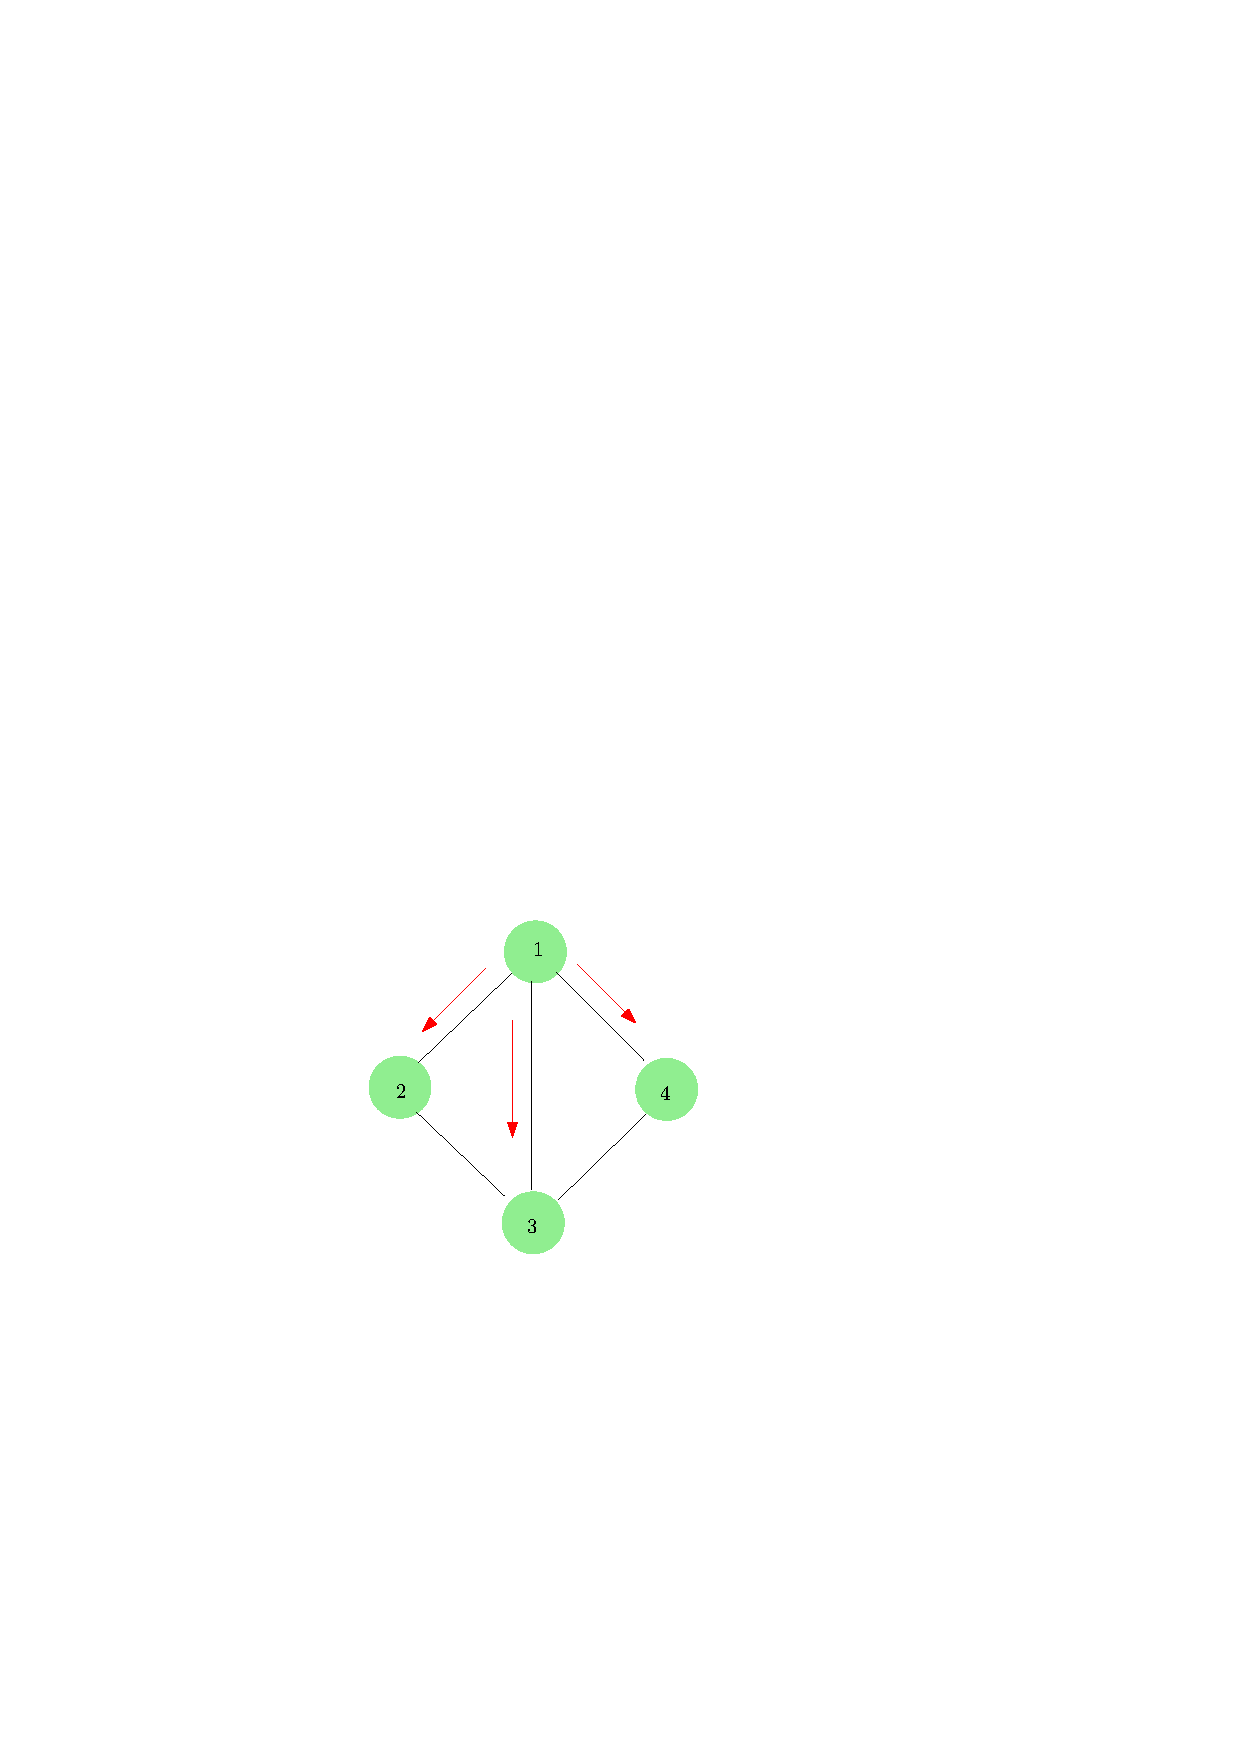
\includegraphics[width=0.32\textwidth]{chapters/background/images/echo/sync/notext_f0_1.pdf}}
    \subcaptionbox{Round Two}{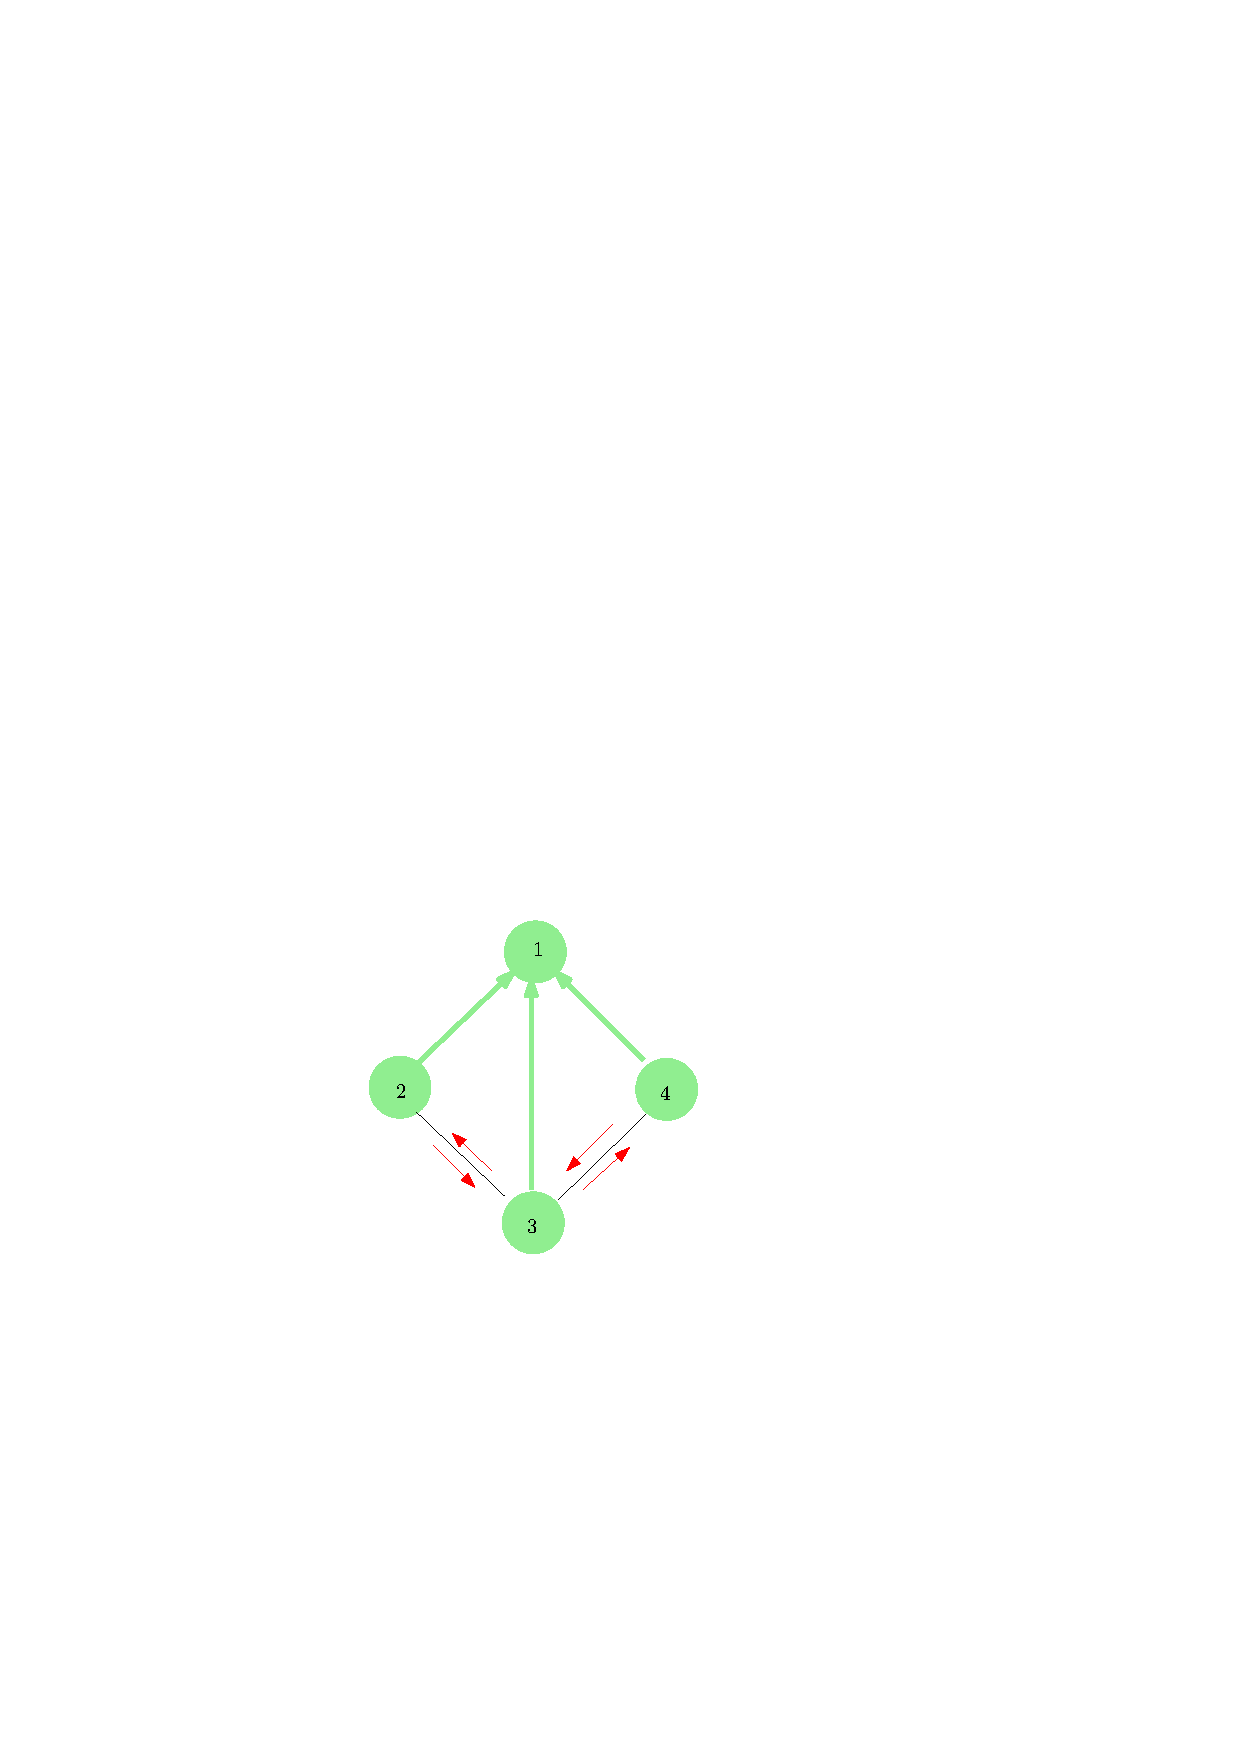
\includegraphics[width=0.32\textwidth]{chapters/background/images/echo/sync/notext_f0_2.pdf}}
    \subcaptionbox{Round Three}{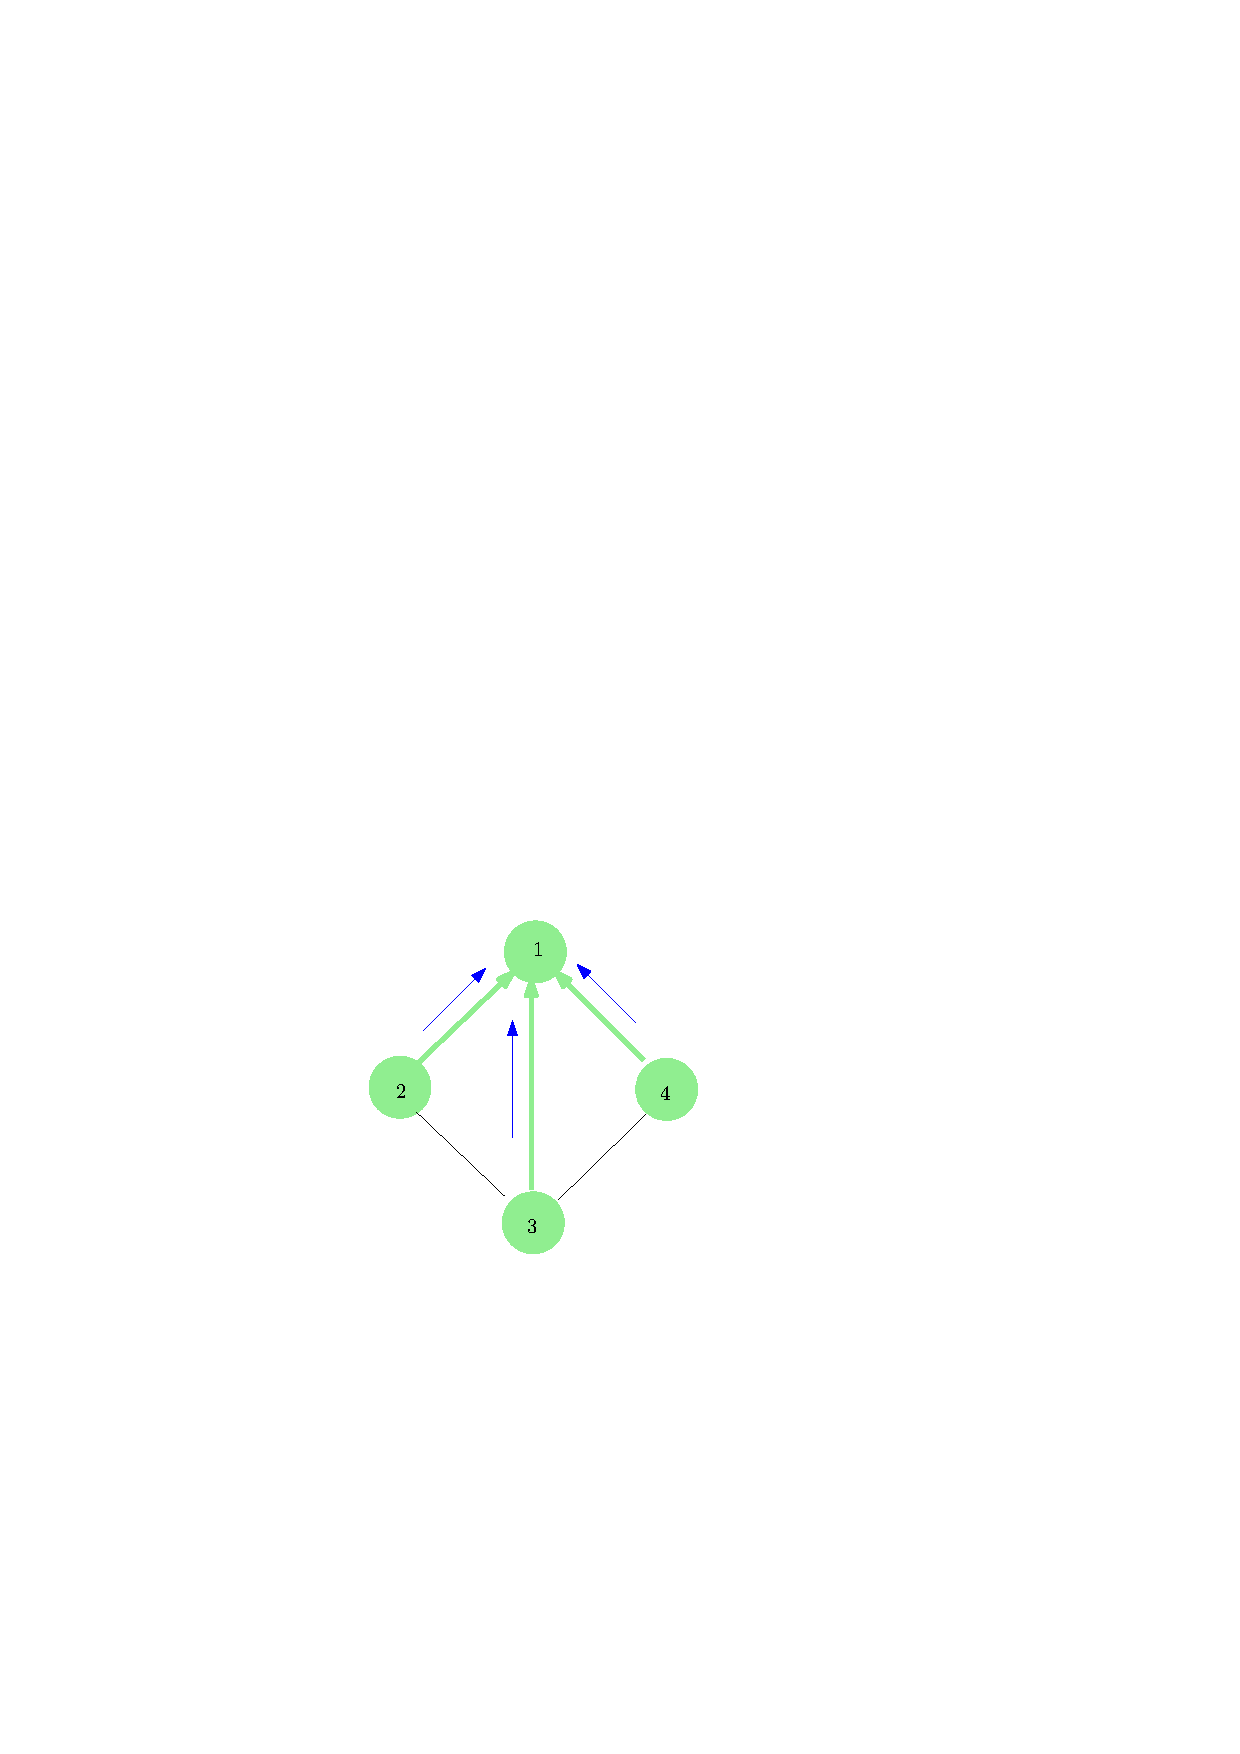
\includegraphics[width=0.32\textwidth]{chapters/background/images/echo/sync/notext_f0_3.pdf}}
    \caption[Progression of the synchronous \textsf{echo} algorithm]{Progression of the synchronous \textsf{echo} algorithm, starting from round zero before any messages are sent.  Arrows in red mean broadcast messages, while arrows in blue mean convergecast messages.}
    \label{fig:back:echosync}
\end{figure}

\begin{figure}[htbp]
    \centering
    \subcaptionbox{Round Zero}{\includegraphics[width=0.32\textwidth]{chapters/background/images/echo/async/notext_f0_0.pdf}}
    \subcaptionbox{Round One}{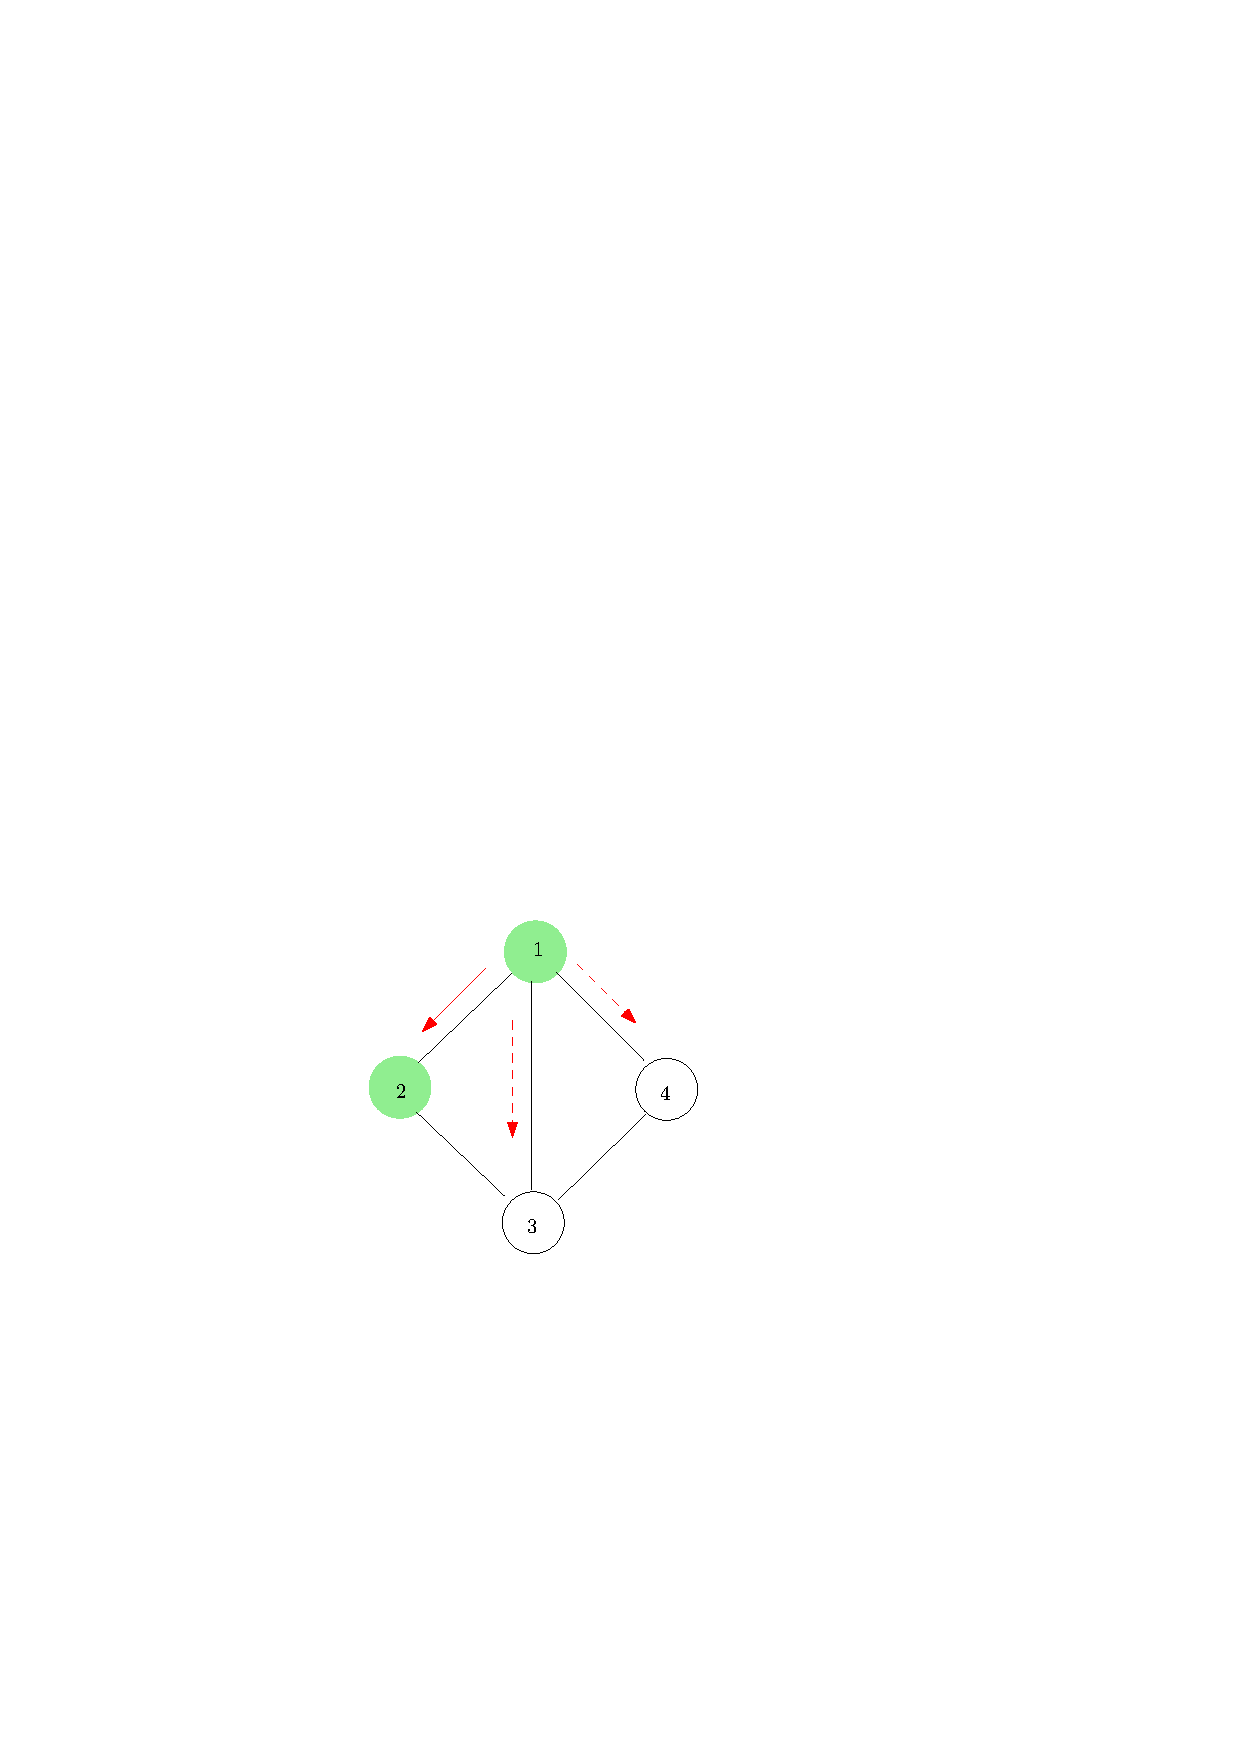
\includegraphics[width=0.32\textwidth]{chapters/background/images/echo/async/notext_f0_1.pdf}}
    \subcaptionbox{Round Two}{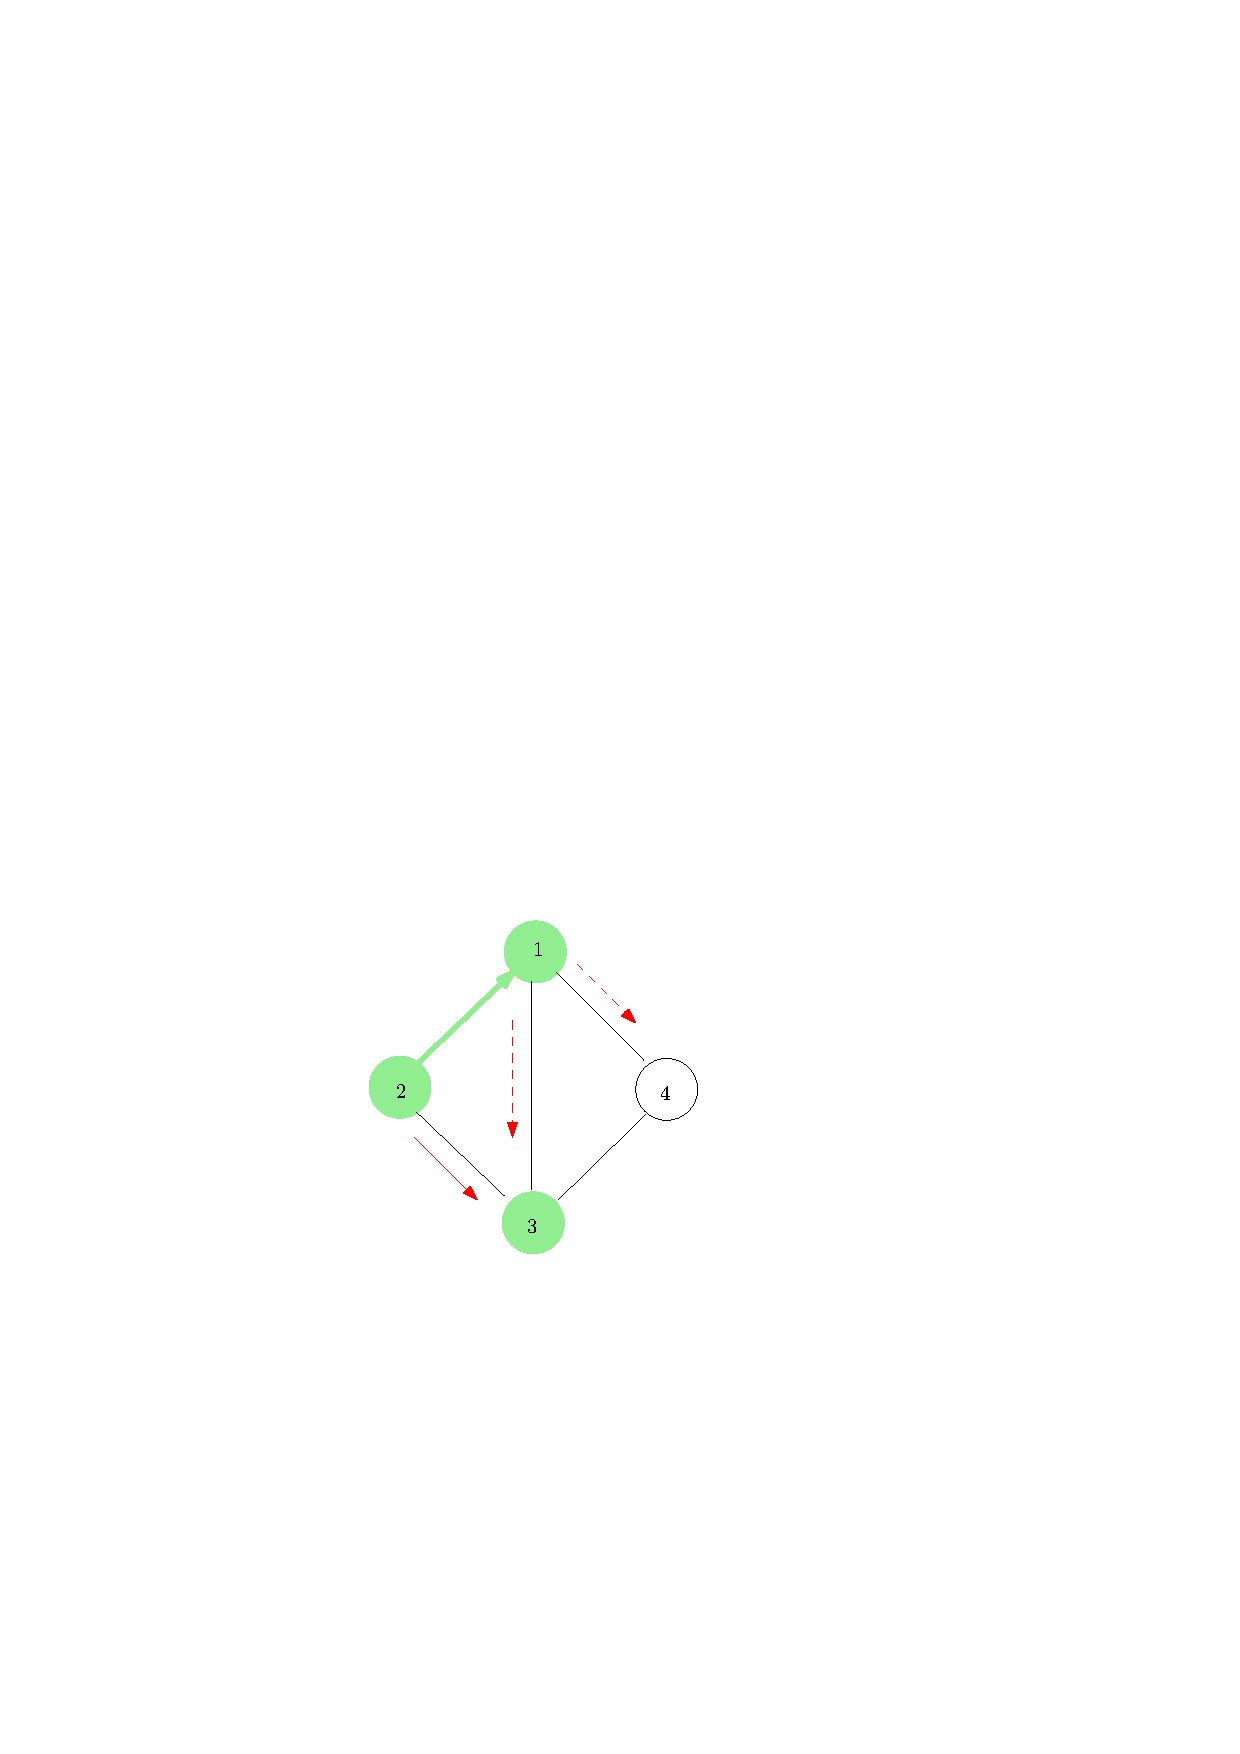
\includegraphics[width=0.32\textwidth]{chapters/background/images/echo/async/notext_f0_2.pdf}}
    \subcaptionbox{Round Three\label{fig:back:echoasync:3}}{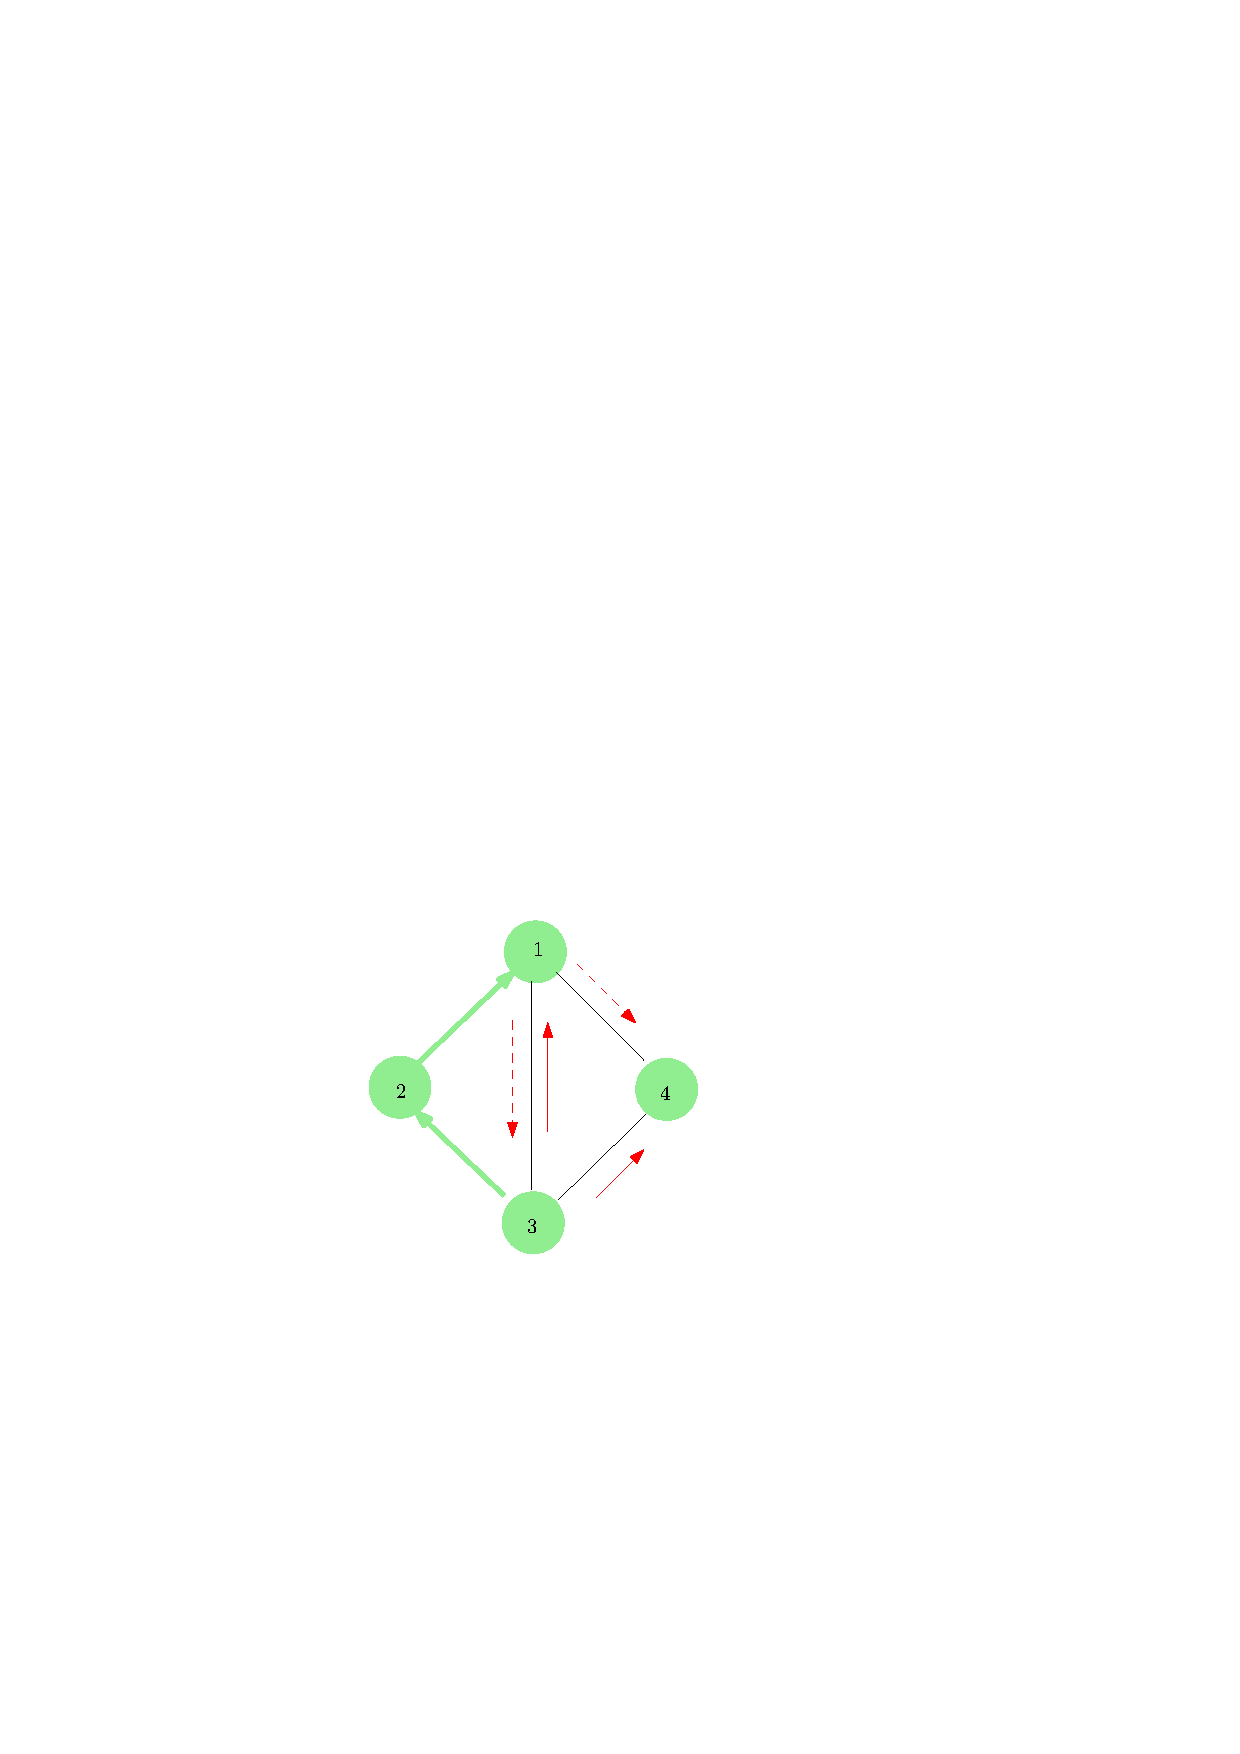
\includegraphics[width=0.32\textwidth]{chapters/background/images/echo/async/notext_f0_3.pdf}}
    \subcaptionbox{Round Four}{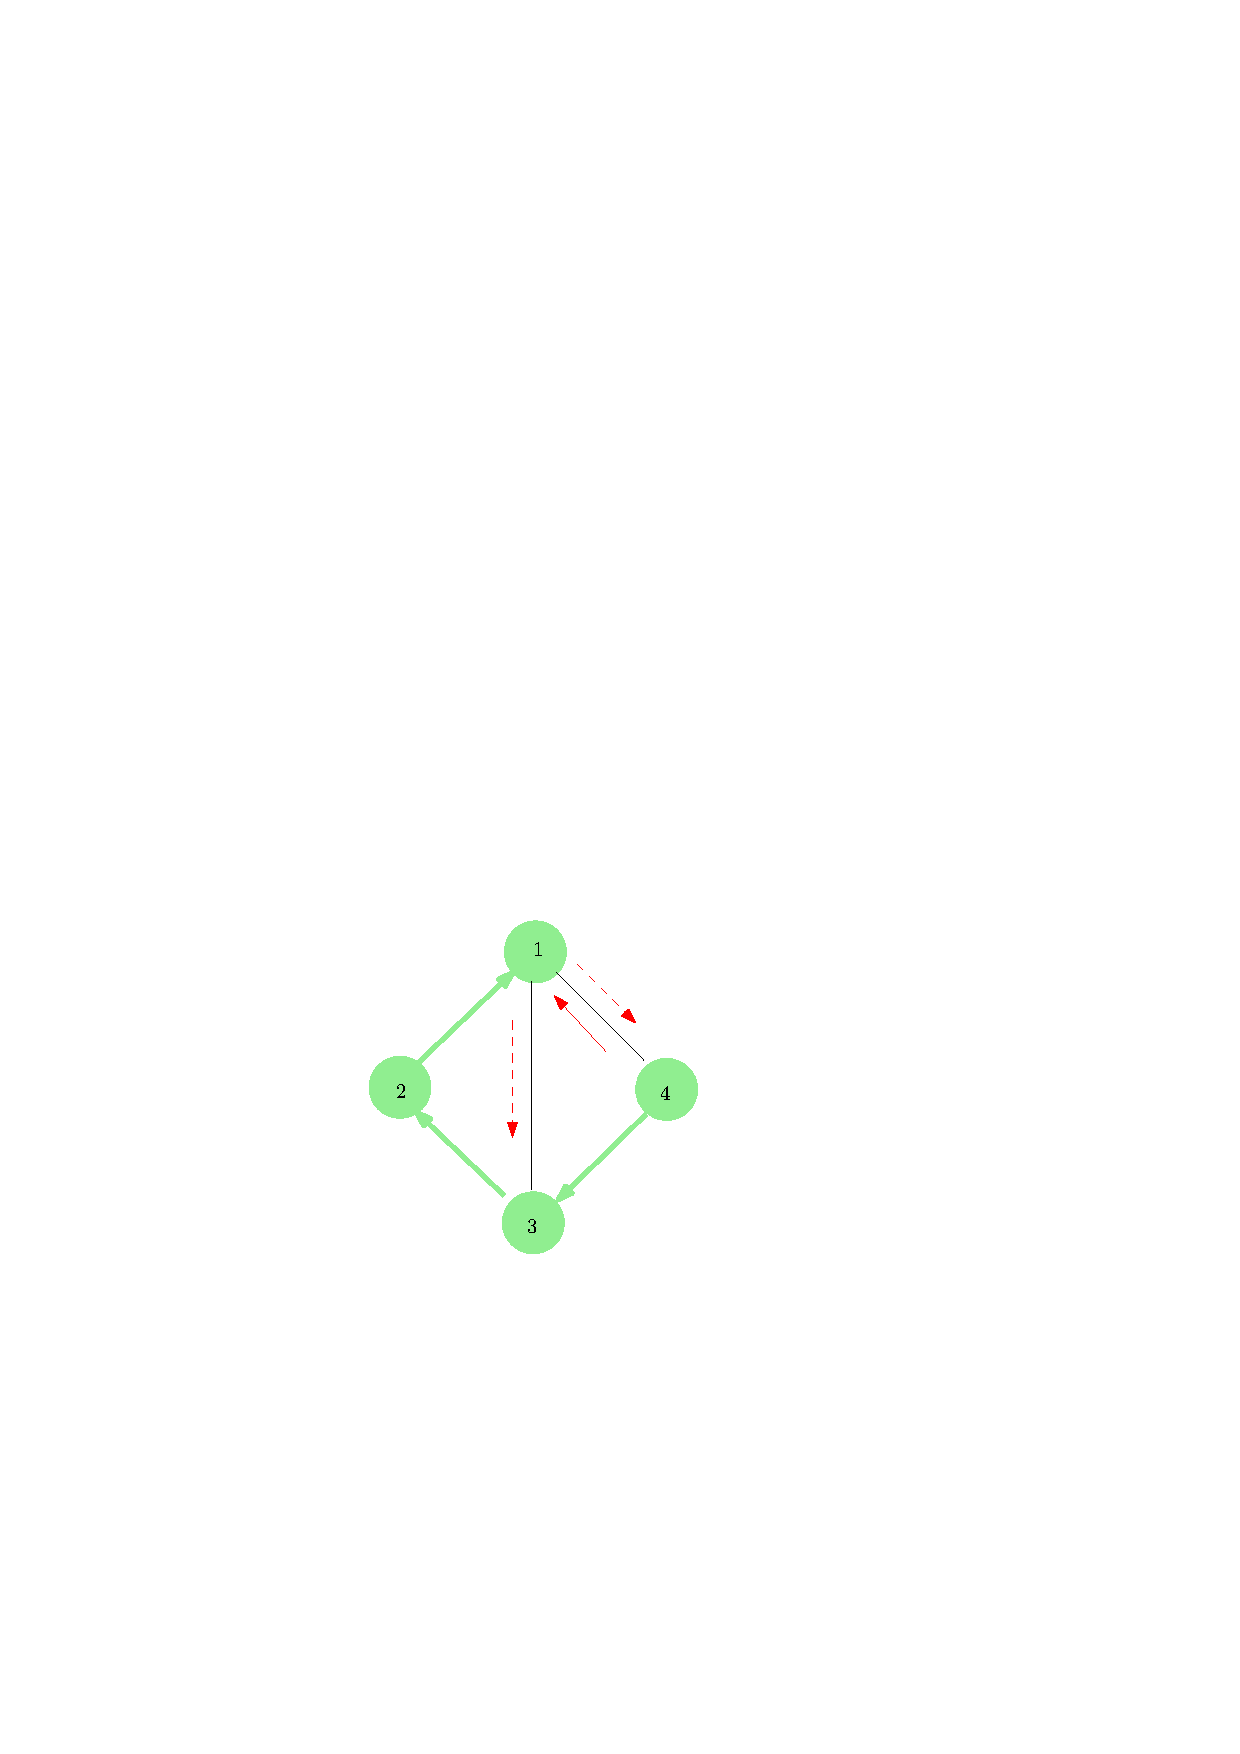
\includegraphics[width=0.32\textwidth]{chapters/background/images/echo/async/notext_f0_4.pdf}}
    \subcaptionbox{Round Five}{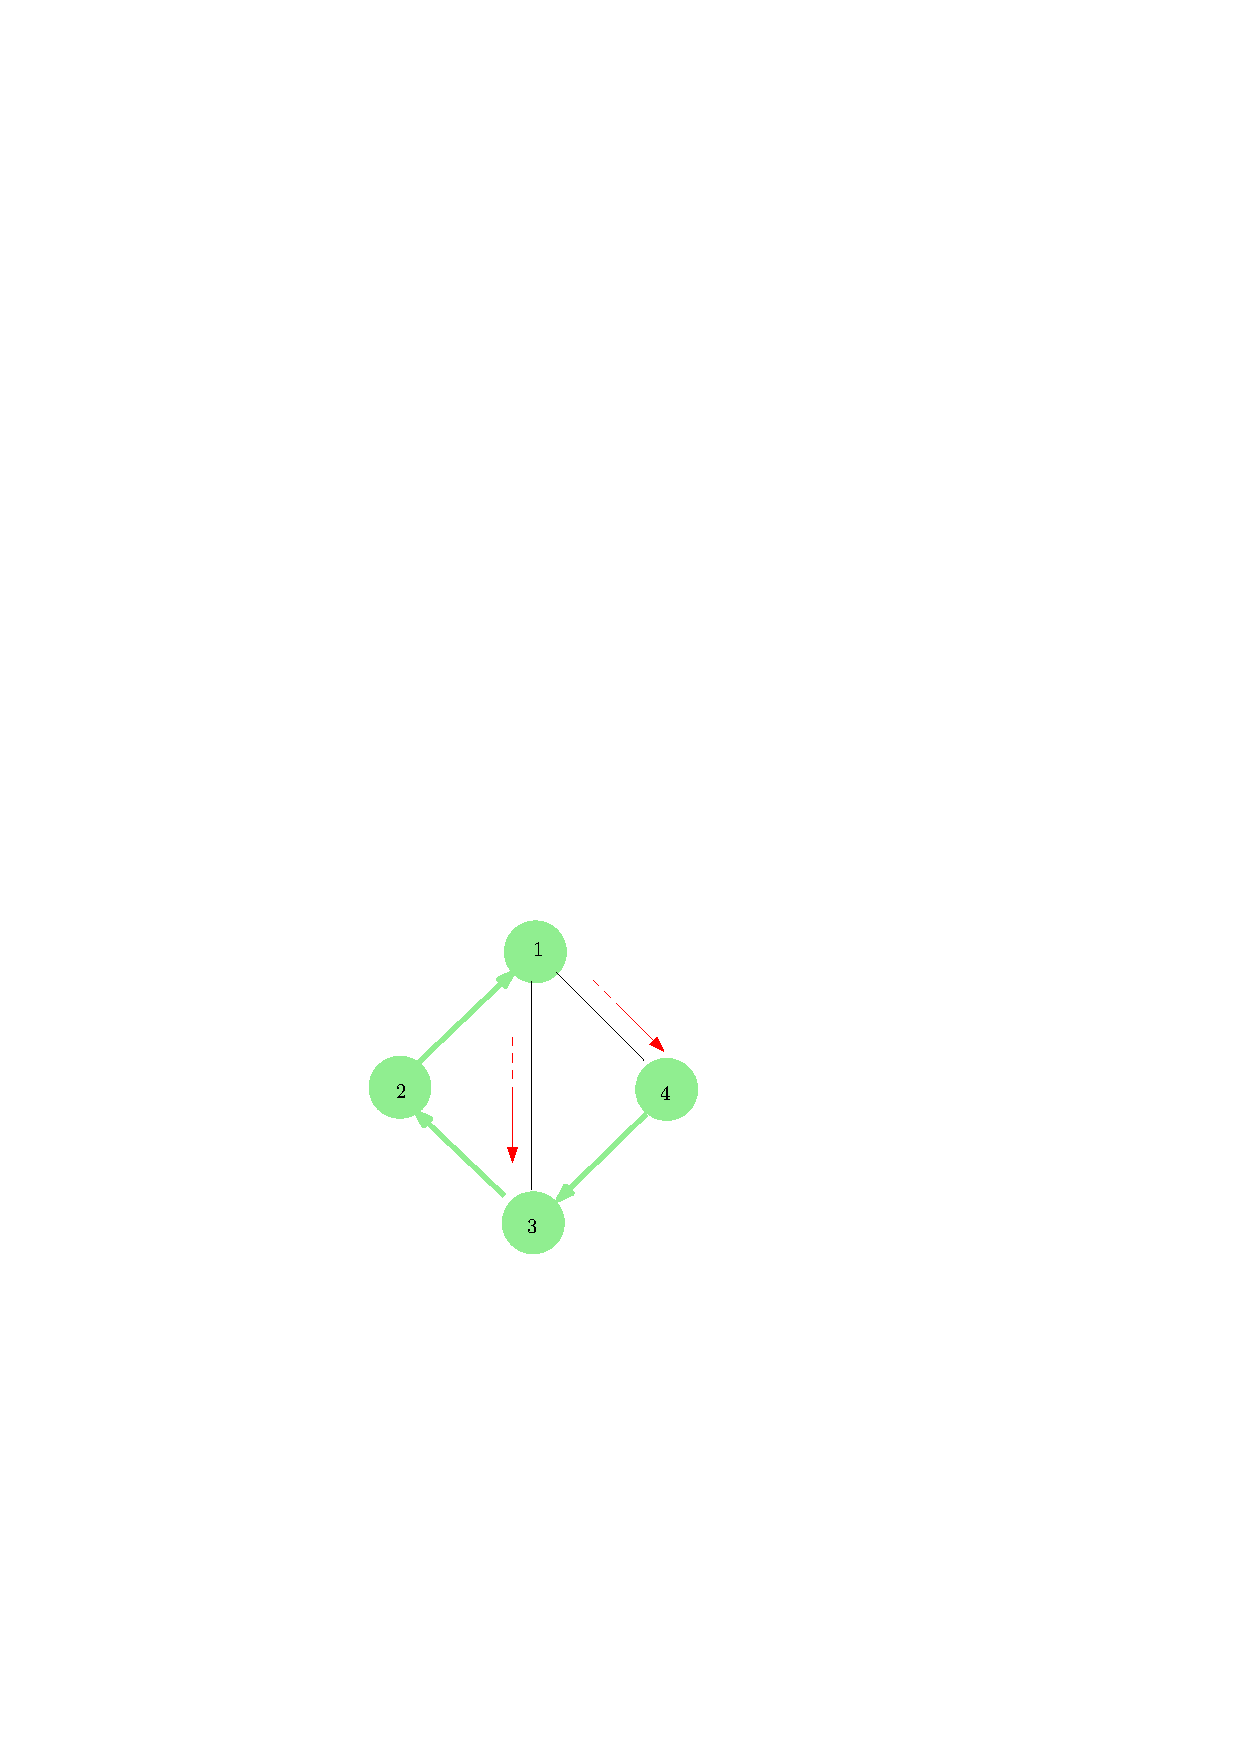
\includegraphics[width=0.32\textwidth]{chapters/background/images/echo/async/notext_f0_5.pdf}}
    \subcaptionbox{Round Six}{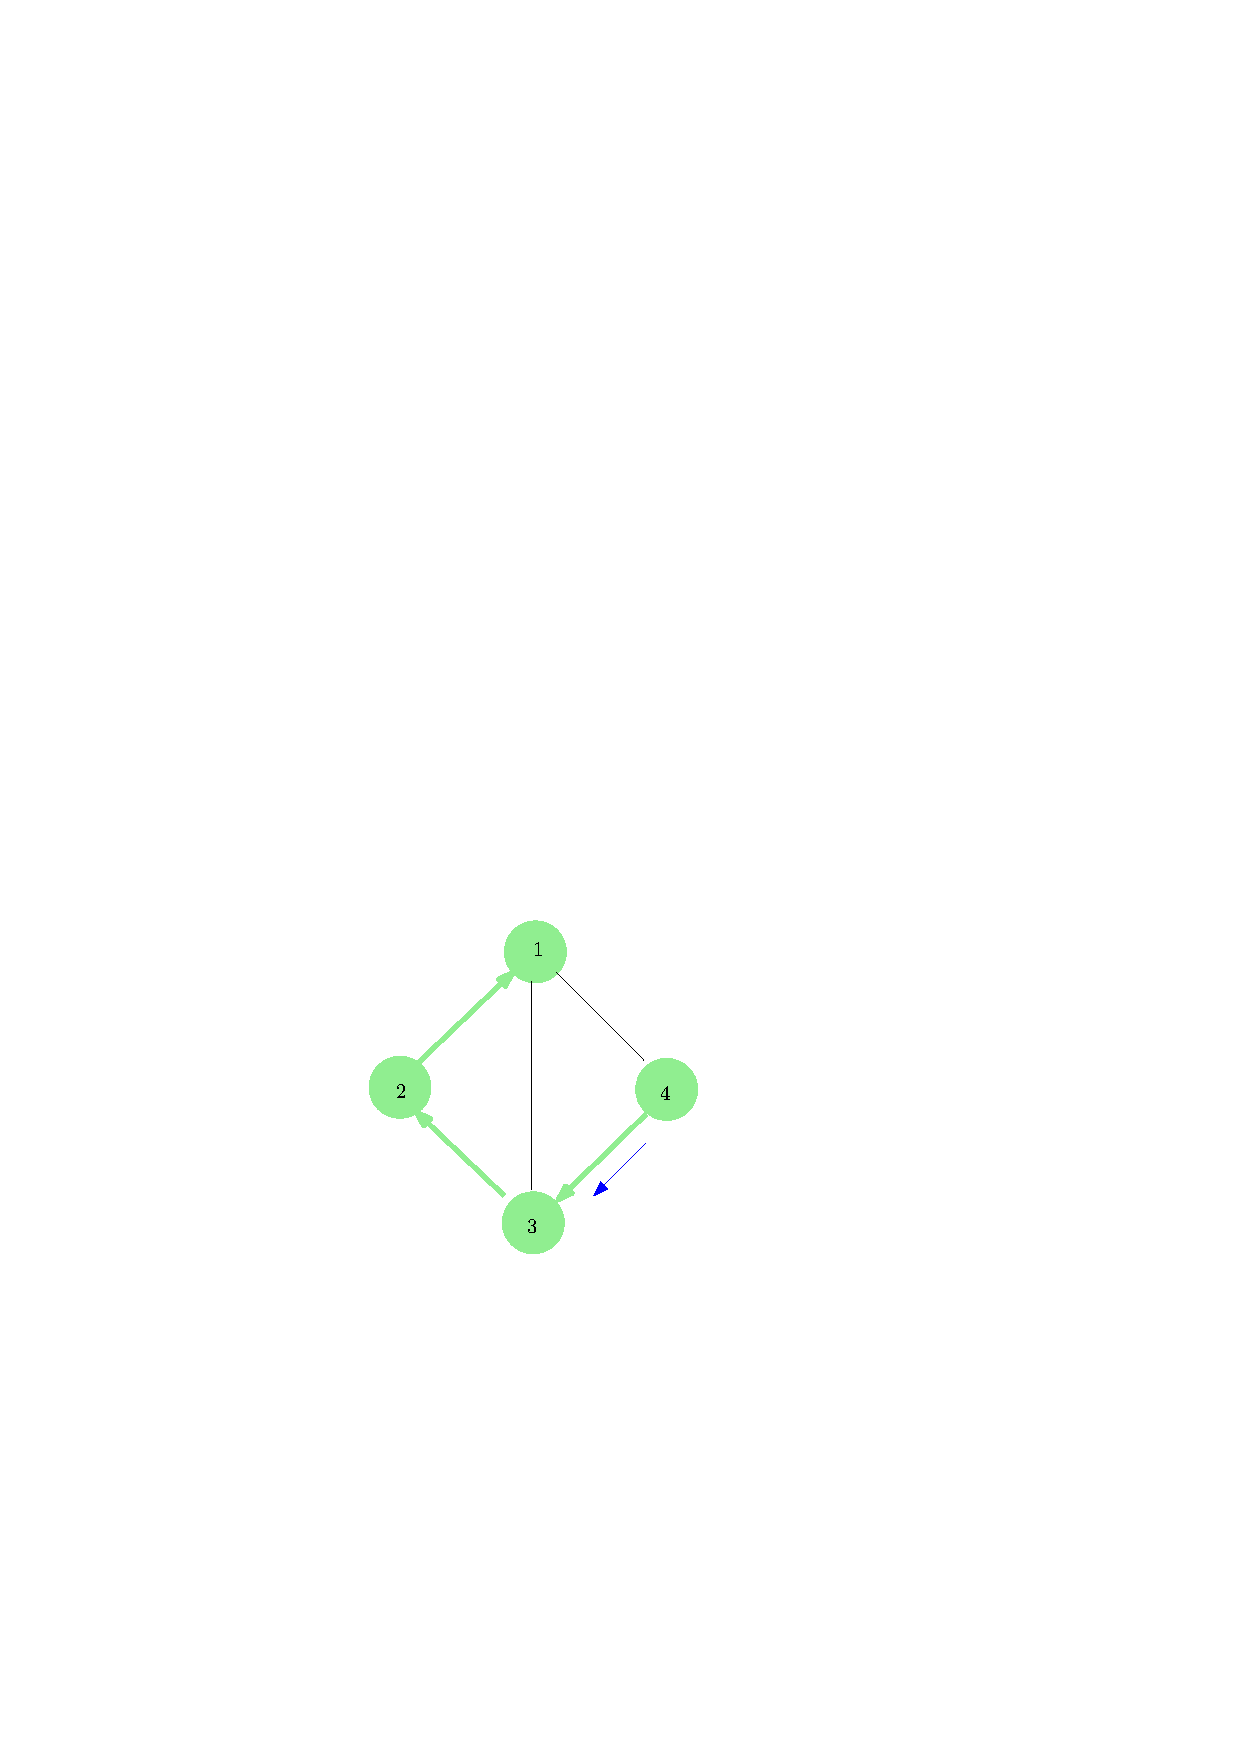
\includegraphics[width=0.32\textwidth]{chapters/background/images/echo/async/notext_f0_6.pdf}}
    \subcaptionbox{Round Seven}{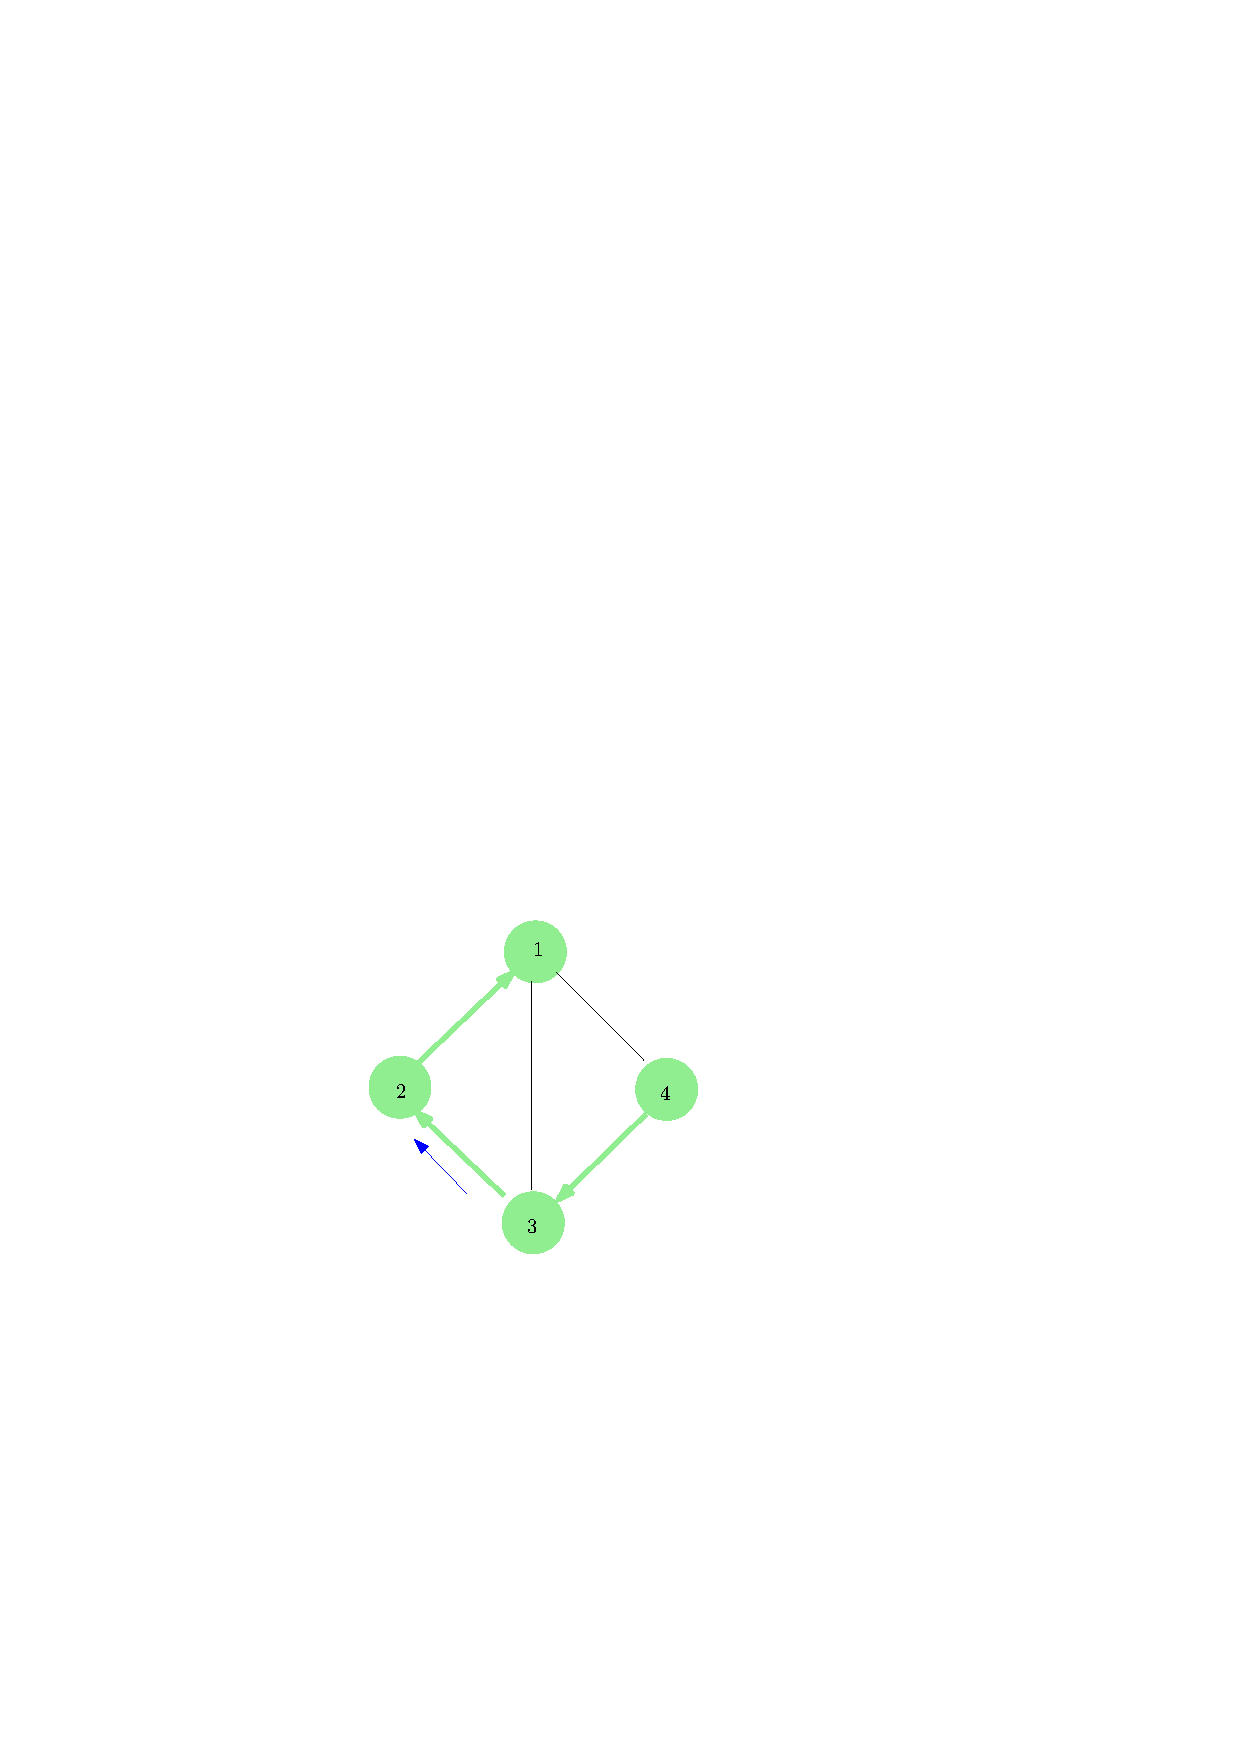
\includegraphics[width=0.32\textwidth]{chapters/background/images/echo/async/notext_f0_7.pdf}}
    \subcaptionbox{Round Eight}{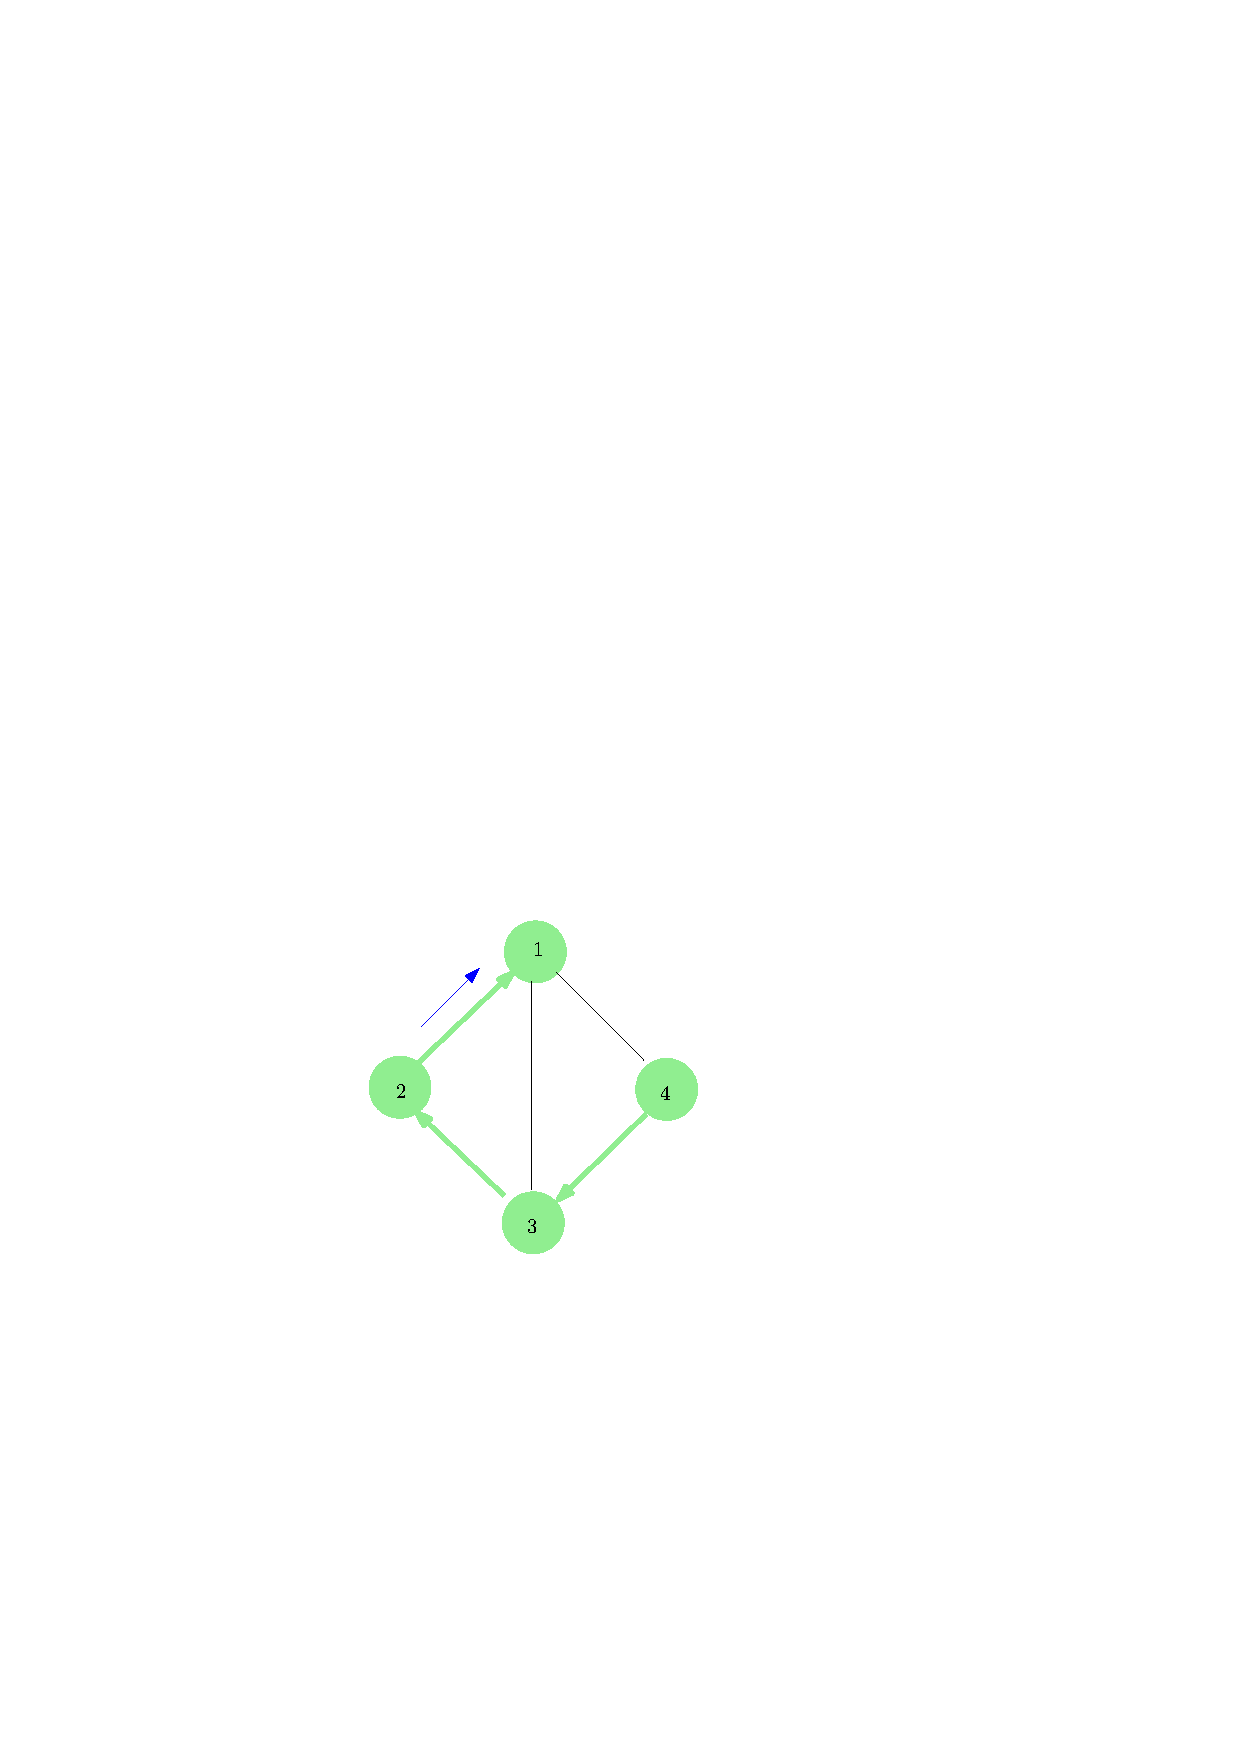
\includegraphics[width=0.32\textwidth]{chapters/background/images/echo/async/notext_f0_8.pdf}}
    \caption[Progression of the asynchronous \textsf{echo} algorithm]{Progression of the asynchronous \textsf{echo} algorithm, starting from round zero before any messages are sent.  Arrows in red mean broadcast messages, while arrows in blue mean convergecast messages.  Despite node 1 being the initiator node, node 4 considers node 3 to be its parent because it first receives a broadcast message from node 3.}
    \label{fig:back:echoasync}
\end{figure}

In the synchronous case, all messages sent out are received simultaneously, and all nodes proceed through their rounds together.  In the asynchronous case, however, messages may arrive at arbitrary times, and nodes proceed through their rounds entirely independently of one another.  The round numbers in the figure mark the point where at least one message has been received by a node.  The nodes react to messages as they arrive, and might do nothing for a time while other nodes are working if no new messages arrive during that time.  Under the asynchronous model, depending on communications topology and speeds, it is possible for the first broadcast message to reach a process to have followed a less direct route from the initiator than otherwise might be possible.  Exactly this is seen in \cref{fig:back:echoasync:3}, where node 4 first receives a message from node 3 (and thus marks node 3 as its parent), despite a direct connection to the initiator, node 1.
\section{\label{sec:back:cml}\glsfmtlong{cml-glossary}}

While parallelism is often the best (perhaps only) way to achieve improvements in execution time for different algorithms once an efficient sequential implementation has been created, it is a notoriously challenging affair \cite{Shun2017}.  When working at the level of directly manipulating threads, such as using the pthreads found in POSIX-compliant operating systems, programmers are exposed to a high level of risk of inadvertently introducing concurrency bugs, such as data races, deadlocks and livelocks.  A panoply of approaches to overcoming this challenge, both theoretical and practical, have been proposed and developed over the years, with varying degrees of success, \eg{} \cite{Boyapati2002,Bocq2012,Seinstra2004}.  Many, perhaps most, large-scale programming languages that use a runtime include some form of parallelism simplification within their standard libraries, \eg{} the Executor system in Java \cite[Ch. 4]{Fernandez2012}, and Swift \& Objective-C's Grand Central Dispatch \cite{Maskrey2018}.

Most simplifications fairly directly target either data-parallelism by simultaneously applying the same operation over multiple elements in arrays, \eg{} SIMD instructions in CPUs \cite{Hughes2015}; or task-parallelism by making provisions for the fork-join model \cite{McCool2012}.  These simplifications can be very useful, but not all instances of parallelism fit neatly into their models.  Algorithms that are well-modelled by the \Gls{csp} and \Gls{actor} models, such as those explicitly centred around concepts of message passing, are not necessarily easy to express using either SIMD or fork-join instructions.

\Gls{cml} \cite{Reppy1991,Panangaden1997} is an approach to concurrent programming originally developed by John Reppy (based on his earlier `Pegasus Meta-Language' \cite{Reppy1988}).  \Gls{cml} was created to provide a framework for creating concurrent programs with synchronous communications on single-core machines,\footnote{In fact, the original implementation \emph{relied} on the fact that the processor was single-core under-the-covers.} and was later extended to permit parallelism \cite{Reppy2009a}.  It was created originally as a library in Standard ML of New Jersey (where ML refers to the earlier programming language \textit{Meta Language}), whence the ML part of the name, but its concepts have subsequently appeared elsewhere.  The basic concept of communicating via channels has experienced a renaissance in recent years, likely due at least in part to its inclusion as a core feature of Go \cite{Meyerson2014}, but \gls{cml} has a more advanced system that Go (at the time of writing) does not fully support.

\Gls{cml} is designed to avoid many of the problems with concurrency that arise in traditional sequential programming, where the use of locks, mutexes and semaphores etc. are frequently required, and often lead to the potential introduction of problems such live-/deadlocks, data races and extreme resource contention.  This is achieved by changing the approach to concurrent programming to one of logically separate, internally sequential processing elements that share data as required by `passing messages'\footnote{This is the logical concept, but there is not strictly any specific required software implementation.} between themselves.  In \gls{cml}, these logical processing elements are referred to as threads, and they exchange messages over channels \emph{synchronously} (called \emph{rendezvous}), \ie{} there is a temporal overlap between one thread offering to send, and another to receive, over the same channel, and the first to offer blocks until the second makes its offer.  When two processes are offering appropriately on either side of an exchange, rendezvous takes place.

Reppy describes a concurrent program as one that supports multiple sequential sub-programs conceptually executing in parallel separately, but interacting through shared resources to achieve a common goal.  \Gls{cml} is concerned with the scenario where said interactions are explicit, and in order to facilitate that \enquote{\gls{cml} takes the unique approach of supporting \emph{higher-order concurrent programming}} (emphasis Reppy's), whereby communication and synchronisation are made into first-class members of the language, similar to how functional programming languages made functions into first-class members of themselves \cite[Preface]{Reppy2007}.

\begin{anfxerror}{Expand this?}
Describe more of how \gls{cml} works?  Is there not something in the gcol chapter that can be shifted into here, at least?
\end{anfxerror}
\section{\label{sec:back:mc}\Glsfmtname{mc}/\glsfmtname{ps}}

\emph{\Gls{mc}}, also known as \emph{\gls{ps}} (the two terms are generally used interchangeably), is a bio-inspired model of computing created by Gheorghe Păun in the late 1990s \cite{tPaun98a,Paun2000}.  It was originally conceived of by considering the process of chemical reactions and exchanges that occur inside living biological cells and the membranes within, and regarding this process as a form of computation.  \Gls{mc} was identified in 2016 by the National Research Council of Canada as \textcquote[][p. 17]{Wiseman2016}{a rigorous and comprehensive framework that provides a parallel distributed framework with flexible evolution rules.}

\citeauthor{Paun2002} describes \gls{mc} as:
\blockcquote[][p.~VII]{Paun2002}{Membrane computing is a branch of natural computing which abstracts from the structure and the functioning of living cells. In the basic model, the membrane systems -- also called P systems -- are distributed parallel computing devices, processing multisets of objects, synchronously, in the compartments delimited by a membrane structure. The objects, which correspond to chemicals evolving in the compartments of a cell, can also pass through membranes. The membranes form a hierarchical structure --- they can be dissolved, divided, created, and their permeability can be modified. A sequence of transitions between configurations of a system forms a computation. The result of a halting computation is the number of objects present at the end of the computation in a specified membrane, called the output membrane. The objects can also have a structure of their own that can be described by strings over a given alphabet of basic molecules - then the result of a computation is a set of strings.}

\begin{anfxerror}{P systems Diagram?}
Include a copy of the membrane layout diagram from Paun?
\end{anfxerror}

\Gls{ps} works analogously to a typical modern electronic computer, in that the system stores data and processes \& updates those data based on a predefined program, with a view to arriving at a computable answer based on the starting state and any inputs to the system \cite{Paun2002,Paun2010b}.  In classical \gls{ps}, the data are multisets of symbols, representing various chemicals and their quantities.  These are found inside one or more \emph{cells},\footnote{Loosely based on real biological cells.} which (to a certain extent at least) form a hybrid between main memory and the processing units of a computer.  The instructions of the program itself are provided by \emph{rules}, which specify transformations of objects and interactions with the surrounding environment and other membranes or cells.

There are now, broadly, three main families of \gls{ps} variants:  \gls{clps} \cite{Paun2001,Paun2002}, \gls{tlps} \cite{tMaPaPaRo01a,Martin-Vide2003} and \gls{snps} \cite{Ionescu2006}.\footnote{Several other variants have been created, but most are used infrequently, if ever.  Most recent work in \gls{mc} has focused on sub-variants of \gls{clps}, \gls{tlps}, \gls{snps} and \gls{cps}.}  \Gls{clps} is the direct descendant of the original classical \gls{ps}, and sees objects compartmented into \emph{membranes}, which are arranged in a graphical tree structure with the outermost \emph{skin} membrane -- which separates the cell from its environment -- as the root of the tree.  In most variants, objects can evolve inside a membrane, but also be communicated between membranes (and the environment).  Furthermore, membranes can \emph{divide} or \emph{dissolve} themselves, and may have one or more special properties, such as \emph{polarization} \cite{Paun1999a}.

On the other hand, \gls{tlps} and \gls{snps} both arrange their computing compartments -- named \emph{cells} or \emph{neurons}, respectively -- as nodes in arbitrary digraphs, with the edges between them representing connecting channels or synapses.  Whereas \gls{clps} emphasises the evolution of multisets of objects inside membranes of a given cell, \gls{tlps} and \gls{snps} emphasise communication between separate cells/neurons, and might not include any capacity for internal evolution inside cells.  If new objects are required, they are imported via communication with the environment, which possesses an unlimited number of all objects but has no rules of its own.

While \gls{tlps} have arbitrary alphabets, only one object is used in \gls{snps}, the \emph{spike}.  This means that \gls{tlps} are frequently much like \gls{clps} in that they have custom objects for each purpose, with the key difference (usually) being in the arrangement of the compartments/membranes/cells relative to each other and the choice between the two motivated primarily by which one better fits the computation to be modelled.

Conversely, \gls{snps} represent everything through the use of differing quantities of the spike, kept in different neurons.  This means that it can be more complex to model certain problems, but also arguably means that \gls{snps} are, \textit{prima facie}, closer to Lambda Calculus \cite{Barendregt1984} and Church Numerals (see \eg{} \cite{Koopman2014,Hinze2005}), as well as Register Machines (see \eg{} \cite{Korec1996}) (and indeed Register Machines have been simulated with \gls{snps} \cite{Pan2010}).  All three main types of \gls{ps}, in some form, have been proven Turing-universal though \cite{Bernardini2005,Chen2008,Freund2005}, so all three should be capable of expressing the same computations in different forms.  Furthermore, because \gls{snps} can be easily represented numerically, they lend themselves well to vector/matrix representations \cite{Zeng2010,Martinez-del-Amor2021,Gheorghe2021,Hu2016}.  This means that, potentially, \gls{snps} implementations can take advantage of high-performance techniques such as directly using \gls{blas} \& \gls{lapack} and/or \glspl{gpu} \cite{Aboy2019}.

Arguably, the most noteworthy and important aspects of \gls{ps} models are that:
\begin{inparaenum}[(i)]
\item They have no space limit.  That is, they contain an unbounded number of cells, objects and membranes;
\item Usually, across all cells and membranes, all rules that can be applied are applied, as many times as possible given the current number of objects available.
\end{inparaenum}
These two features mean that \gls{ps} have unbounded space and processing capacity, which can be used to solve traditionally computationally difficult problems relatively quickly \cite{Sosik2003,Jimenez2003,Paun1999a,Henderson2020}.  Most of these solutions, however, rely on trading time complexity for space complexity.  While this works in the theoretical framework, electronic simulations of the systems do not have access to unlimited instantaneous memory space, meaning many of the fast solutions are impractical with current real-world computers, \eg{} \cite{Cooper2019,Cooper2019a} \fxnote[inline]{[refs]} (see further \vref{sec:psystemsuses}).

\citeauthor{Valencia-Cabrera2019} said of this:
\blockcquote[][p.~213]{Valencia-Cabrera2019}{We do not know if we will have those machines able to solve NP-complete problems in polynomial time, in many cases even linear time, but \textins{that does} not necessarily mean we will have to wait until that moment in biochemical technology to find some relevant use of P systems. As Babbage kept working on his ideas, not simply waiting until the precise moment when Turing, Von Neumann, and their contemporaries witnessed the first electronic computers based on similar principles, membrane computing must keep moving, finding new ways to provide a step further.}

Nevertheless, modelling a problem in \gls{mc} can lead to new insights or improved formulations of solutions, as occurs in \cref{chap:nmp}.  For example, in \cite{GimelFarb2013a} (building on \cite{Gimelfarb2011}) \citeauthor{GimelFarb2013a} describe how formulating Symmetric Dynamic Programming \gls{sm} in terms of \gls{ps} led to finding a bug in the implementation, \textcquote[][p.~24]{GimelFarb2013a}{but also (and what is much more important) refactor this algorithm, based on our cell structure.  The result is a more robust and flexible version, which allows us to fine tune its parameters and enhance its capabilities, without rewriting it from scratch.}  Furthermore, as reported in \cite{Nicolescu2014b}, this exercise led directly to the creation of a new \gls{sm} algorithm, Concurrent Propagation \cite{Gimelfarb2012}.  \citeauthor{Pang2018} \cite{Pang2018} also claim significant benefits from modelling certain problems in a novel variant of \gls{enps} \cite{Pavel2010}, but it is unclear how much of the stated benefit compared to their baseline implementation arises instead from the use of a \gls{gpu}.

\subsection{Objects, Rules and Steps}
All known \gls{ps} types fundamentally operate on a similar basis:  One or more sets of rules -- \emph{\gls{ruleset}} -- are defined, describing how the \emph{objects} present in the system's compartments change at each \emph{step}.  As mentioned above, the objects are usually multisets of arbitrary symbolic \emph{atoms}, with the exceptions of \gls{snps} which uses the spike as its only symbol, and Numerical \gls{ps}, which uses ordinary numbers in place of atoms.  Certain systems may introduce other object types as required.

\Gls{ps} types normally operate synchronously and assume the presence of a global clock.  At each clock ``tick'', every compartment compares its extant objects and its \emph{evolution rules}, determines which rules are applicable given the current objects, and then deletes the objects used in the rules, replacing them with new ones as the rules dictate.  This process comprises a step.  The progressive execution of the system's rules over multiple steps is referred to as the system's evolution.

All \gls{ps} evolve, and therefore all types have evolution rules (though they may not be referred to as such).  Other types of rules are possible, including: \emph{dissolution} and \emph{division} rules in \gls{clps} and \gls{tlps}, where membranes either dissolve and release their objects into the their parent membrane, or replicate themselves (essentially performing mitosis) and distribute their contents among the new membranes; \emph{forgetting} rules in \gls{snps} whereby one or more copies of the spike are removed from a given neuron; or, splicing rules in Splicing \Gls{ps}\footnote{Particularly notable for working over strings of an alphabet, instead of multisets.} \cite[Ch.~8]{Paun2010b}.

All rules use the same basic model.  At the start of a step, they check if the necessary pre-conditions for the rule are met.  If they are, then any changes to the state of the system specified by the rule occur.  It is common for rules to remove or delete some objects in the relevant compartment, and instantiate new ones.  It is typically assumed that all objects are deleted or created instantaneously at the last moment of the rules' execution.

Generally, rules are specified in the form \textsc{\gls{lhs}} \(\rightarrow\) \textsc{\gls{rhs}}, where objects to be removed (the presence of which are therefore a precondition) are written in the \gls{lhs} and the objects to be created are written in the \gls{rhs}.  Unless otherwise specified, it is typically assumed that all rules which can be applied at a given step are applied.

\subsubsection{Weak Priority Order}

Many, perhaps most, types of \gls{ps} \glspl{ruleset} use a \emph{weak-priority} ordering.  This means that some rules will be tested for applicability ahead of others, on some priority basis, but earlier applicable rules only prevent later applicable rules from being applied if there is a conflict between the two.  The most common way that this conflict can arise is by two rules trying to use the same pre-existing object in the compartment.

Generally speaking, an individual rule will select for use one or more copies of one or more objects the multiset.  At the end of the rule's application, these objects are deleted and replaced with any new ones the rule specifies.  Since the rule will delete the chosen objects, it would not make sense for another rule to be able also to use and then delete the same objects.  Therefore, the first rule to select (or take hold of or seize \etc{}) a given object prevents any other rule from using it too, and thus the first rule has priority over later rules.

The typical method of defining rules' priority is to use \emph{top-down} ordering.  This simply means that the rules presented first in a \gls{ruleset} have priority over those rules presented further down.  The basic process to determine which rules to apply is therefore a sequential one.  Starting with the first rule, and proceeding with each successive rule in turn, test if the rule is applicable at all.  If it is, set it to be applied during the step as many times as possible depending on the rule, the objects present, and the run-time mode (see \eg{} \cref{sec:cps:applicationmodes} for a discussion of this in relation to \gls{cps}).

Any objects now set to be deleted by a previous rule are then unavailable to a later rule, but if there are sufficient remaining objects for that rule to apply, it still may, giving a \emph{weak} priority to the earlier rules.  The application of an earlier rule does not guarantee that a later rule will not apply, but the earlier rule takes precedence in the case of a conflict.  Furthermore, some \gls{ps} variants, \gls{cps} included, use states on their compartments (or the system as a whole).  In this case, rules will usually state a necessary starting state, and an ending state to which the rule transitions the system.  The first such rule to apply dictates the ending state of the compartment (or system) at the end of the step.  Rules with a lower priority may then only be applied if they have the same requisite ending state.

%%%%%%%%%%%%%%%%%%%%%%%%%%%%%%%%%%

\subsection{Computer Representations and Simulations of \glsfmtname{ps}}

\subsubsection{\Adhoc{} and General Simulations}
There are arguably two main approaches to simulating \gls{ps}:
\begin{inparaenum}[a)]
\item ``\Adhoc{}'' simulations, where a separate program is written specifically for a given type of problem and its \gls{ps} solution; and
\item ``General'' simulations, where a separate simulation engine capable of simulating one or more types of \glspl{ps} is created independent of a given problem, and is supplied problem-specific configurations.  The engine uses the configuration to initialise the simulated system, and works through the problem from there.
\end{inparaenum}

The main advantage of the \adhoc{} style is the ability to adjust and optimise the simulation's implementation to suit the \gls{ps} variant used, and the problem at hand.  In general, \adhoc{} simulations would be expected to require less resources to find the answer, \eg{} running faster and/or using less memory.  The major disadvantage of the \adhoc{} approach is that a new simulation must be developed for each problem studied, requiring more time and greater levels of technical skill while reducing flexibility.  The main advantages of the general approach are greater flexibility from the produced program -- \ie{} it can simulate more problems -- and a broadening of the people who can experiment with different \gls{ps} variants and problems to those with lower levels of programming expertise.

General simulations permit specialisation and a division of labour, meaning one person can look into new \gls{ps} variants and problems to apply them to, while another person focuses on developing and improving the simulation engine itself.  This is a clear upside, but there is equally a downside: lacking problem-specific knowledge, the general simulations usually do not perform all potential optimisations, meaning that there could be unavoidable upper bounds on the efficiency of a simulation, no matter the specific problem at hand.  Furthermore, general simulations must run inside another program, whereas \adhoc{} simulations can be created as independent, native executables.

Traditionally, this has been an `either/or' problem, where one can take either a wholly \adhoc{} approach or a wholly generalist approach.  \citeauthor{Perez-Hurtado2019} more recently introduced a \gls{ps} ``compiler'' \texttt{pcc} \cite{Perez-Hurtado2019}, which can produce a standalone native executable from a non-programmatic specification of a particular \glspl{ps} --- thus providing a third, middle-ground option.  They say of this compiler: \textquote{the goal of \textins{\texttt{pcc}} is twofold: On the one hand, it purports to be a good assistant for researchers while verifying their designs, even working with experimental models. On the other hand, it provides optimized simulators for real applications, such as robotics or simulation of biological phenomena.}  It was not used in this dissertation, as \texttt{pcc} did not support \gls{cps} at the relevant time, but the idea holds great promise for the future.

%%%%%%%%%%%%%%%%%%%%%%%%

\subsubsection{\label{sec:back:simulators}\Glsfmtname{ps} Simulators}

\citeauthor{Valencia-Cabrera2019} provide a summary of the development of simulators for \Gls{ps} since the field's inception in the late 1990s \cite{Valencia-Cabrera2019}.\footnote{The authors also provide a timeline of practical works in \gls{ps} at \url{https://github.com/RGNC/plingua}.  Some of the software described in this \lcnamecref{sec:back:simulators} is available at \url{http://ppage.psystems.eu/index.php/Software/}.}  Unsurprisingly, most early simulators were \adhoc{} and created for a specific purpose, focusing on one problem domain and simulating one \gls{ps} variant.  Many were intended for formal verification of models as much as they were for practical use \cite{Gutierrez-Naranjo2007}.  These early simulations were written in a wide variety of programming languages, including (comparatively) lesser-used languages such as Haskell, Prolog and LISP.  Notably, \citeauthor{Ciobanu2004} created a simulator specifically for distributed computing, using C++ and \gls{mpi} \cite{Ciobanu2004}.

As the number of \gls{ps} variants defined, and simulations to experiment with them, expanded greatly, it began to make more sense to create general simulators which did not require detailed customisation for every experiment.  A handful of these multi-purpose simulators began to appear, including (among others): PSim \cite{Bianco2007,Bianco2007a}; a transpiler from Systems Biology Markup Language (SBML) to C Language Integrated Production System (CLIPS) \cite{NepomucenoChamorro2005};  and a web-based simulator which also made use of CLIPS \cite{Bonchis2005}.  Of particular interest from this period is \cite{Acampora2007}, which specifically targeted the creation of a paralel and distributed multi-agent system, to take advantage of the concurrency inherent in most \gls{ps} variants and models.

While these simulators were a clear step to re-usability, they still largely targeted only a specific \gls{ps} variant or sub-variant.  There was another issue in that there was no standard for representing an individual \glspl{ps}.  Simulators generally either used their own custom specification system, such as a special-purpose XML schema, or attempted to make use of a representation created for another purpose, such as SBML.  To address these two shortcomings of the existing systems, researchers at the Universidad de Sevilla (University of Seville) in Spain created \gls{plingua}\footnote{\url{http://www.p-lingua.org/wiki/index.php/Main_Page}, \url{https://github.com/RGNC/plingua}} \cite{Diaz-Pernil2008a,Garcia-Quismondo2010} and \gls{mecosim}\footnote{\url{http://www.p-lingua.org/mecosim/}} \cite{Perez-Hurtado2010}.

\Gls{plingua} is a declarative markup language, used to specify specific systems and their initial configurations.  Arguably, it has become the dominant specification language of the computerised \gls{ps} world.  Crucially, \gls{plingua} also allows for the specification of new \gls{ps} variants and extensions to existing ones, giving it a much greater potential flexibility.  It is primarily built around the Java library PLinguaCore, which provides functionality to translate between various representations of \gls{ps} specifications.  One of the simulators to make heavy use of \gls{plingua} is \gls{mecosim}.

\Gls{mecosim} is a Java-based general-purpose \gls{mc} simulator.  It uses \gls{plingua} and spreadsheets to define the evolution of a given \gls{ps} type, as well as the problem to be solved --- both the rules and starting state of the system.  The particular strengths of \gls{mecosim} are that, once a particular type of \glspl{ps} has been defined it is completely re-usable, and the simulator permits rapid experimentation with different designs without any programming.  Sadly, however, it appears that both \gls{plingua} and \gls{mecosim} have effectively been abandoned, as neither seems to have been substantively updated in some years.  It is not currently clear if there is any unifying simulator or specification language to supersede them.

In \cite{Raghavan2020a} \citeauthor{Raghavan2020a} described frustration with a lack of interoperability among the then-extant handful of description and simulation tools for \gls{enps}.  The authors created a tool that could translate between input representation formats -- primarily one based on XML, and another custom one, \fxerror{ref?}{PeP}, created specifically for \gls{enps}.  A second goal of the work was to permit the transfer of the output from one system as the input to another, \ie{} not just moving numbers between membranes, but transferring results between wholly different systems.  This means that they can form a series of systems into a processing pipeline without manual intervention.

\citeauthor{Raghavan2020} \cite{Raghavan2020} sought to improve upon \citeauthor{Florea2018}'s work \cite{Florea2018} and implement a simulator for \gls{enps} that would run on a \gls{gpu}.  Given that \gls{enps} directly use numbers, rather than going through an abstract representation of them such as unary arithmetic, this makes a great deal of sense.  The devised system translates PeP representations of given \gls{enps} problems to \fxerror{ref?}{CUDA C}, and runs them on an NVIDIA \gls{gpu}.\footnote{CUDA, being an NVIDIA product, is only supported for their own \glspl{gpu}.}  Experimental results suggested that the systems involved did not need to be particularly large for the overheads involved in using CUDA to outweighed by the significant parallelism opportunities.  The authors found a maximum speed-up against \cite{Florea2018} of 770 times on their largest test system, with at least an order of magnitude improvement in almost all other tests.

Even more historic simulation software for \gls{mc} is listed in \cite{Raghavan2016}, but the ones not mentioned above were not considered significantly noteworthy or long-lived enough to merit special mention.  Most of these simulators seem to have been created simply to support only one or a handful of papers, and (if even still available) have received no maintenance in years.  Nevertheless, the curious reader might still find something to interest them.

%%%%%%%%%%%%%%%%%%%%%%%%%%%%%%%%%%%%%%%%%%%%%%

\subsection{\label{sec:psystemsuses}Practical Applications of \glsfmtname{ps}}
\Gls{mc} is not just a theoretical model with limited practical use.  Besides Image Processing \& Computer Vision (see \vref{subsec:imgprocpsys}), \gls{ps} variants have been applied to a range of fields, from power grid management to robotic control systems \cite{Zhang2017}.

\begin{anfxwarning}{Some citations to include}
\cite{Zhang2020,Colomer2010,Gheorghe2010,Liu2016,Huang2016,Perez-Hurtado2010,Verlan2012,Syropoulos2004,Liu2020,Lefticaru2011,Oltean2008}
\end{anfxwarning}

\begin{anfxerror}{Finish this}
\citeauthor{Florea2017} proposed using Enzymatic Numerical \gls{ps} for robotics \cite{Florea2017,Florea2016,Florea2017a,Florea2019,Florea2016a}.
\end{anfxerror}

%%%%%%%%%%%%%%%%%%%%%%%%%%%%%%%%%%%%%%%%%%%%%%%%

\subsubsection{\glsfmtname{ps} on \glsxtrlongpl{gpu}}
In many instances, a \gls{ps} model for a problem involves many independent small elements processing their data separately, and perhaps updating each other's state at the end of a step.  Given that this sounds remarkably close to the Single-Instruction Multiple-Thread \cite[Ch. 4.4.1]{Hennessy2012} nature of modern \gls{gpgpu}, it is no surprise that there has been much work put into simulating \gls{ps} on \glspl{gpu}.

\begin{anfxwarning}{More citations}
\cite{Cecilia2010,Cecilia2010a,Cecilia2013,Macias-Ramos2015,Martinez-Del-Amor2015,Martinez-Del-Amor2013a,Maroosi2014,Maroosi2014a}
\end{anfxwarning}
\glsresetall
\newcounter{rulesnumber}

% --------------------------------------------------------------
\chapter{\label{chap:nmp}Neighbourhood Message Passing}

\section{Introduction}
This \namecref{chap:nmp} presents a framework for passing messages between discrete points on a finite lattice, where each point updates its internal data (and thus the messages it sends) based on messages received.  Each point is uniquely connected to other points and so has its own \emph{neighbourhood}, being the specific other points it communicates with.  A key aspect of this \emph{\gls{nmp}} computation is that the messages to a given neighbour depend upon the messages received previously from \emph{all} neighbours, \emph{except} the neighbour to which the current message is sent.    This necessarily means that in \gls{nmp} each grid location must have at least two neighbours; a single neighbour cannot form a meaningful neighbourhood.  This \namecref{chap:nmp} focuses on the \emph{square grid lattice}
but the principles of \gls{nmp} apply equally to all lattices.%focuses on the \emph{square grid lattice} but \gls{nmp} applies equally to lattices of any shape, dimension, or connectivity.

In this \namecref{chap:nmp}, the individual computational units in the lattice are termed \emph{\glspl{pe}}.\footnote{The short form ``\gls{pe}'' is derived from “processing element'' in the same way that “pixel'' is derived from “picture element''.}  These are the logical base units for computation for \gls{nmp} and are represented by \gls{cps} \glspl{tlc}.  A visual example of the \gls{nmp} process for the \emph{\gls{fne}} on the square lattice is shown in \cref{fig:nmp:gridmessaging}.  A \gls{pe} in the grid received messages from its neighbours to the left, right, and bottom at generation \(t - 1\), and used the data from those messages to prepare its new message to be sent to the neighbour above at iteration \(t\).  The same is performed for every other neighbour too.

\begin{figure}
    \centering
    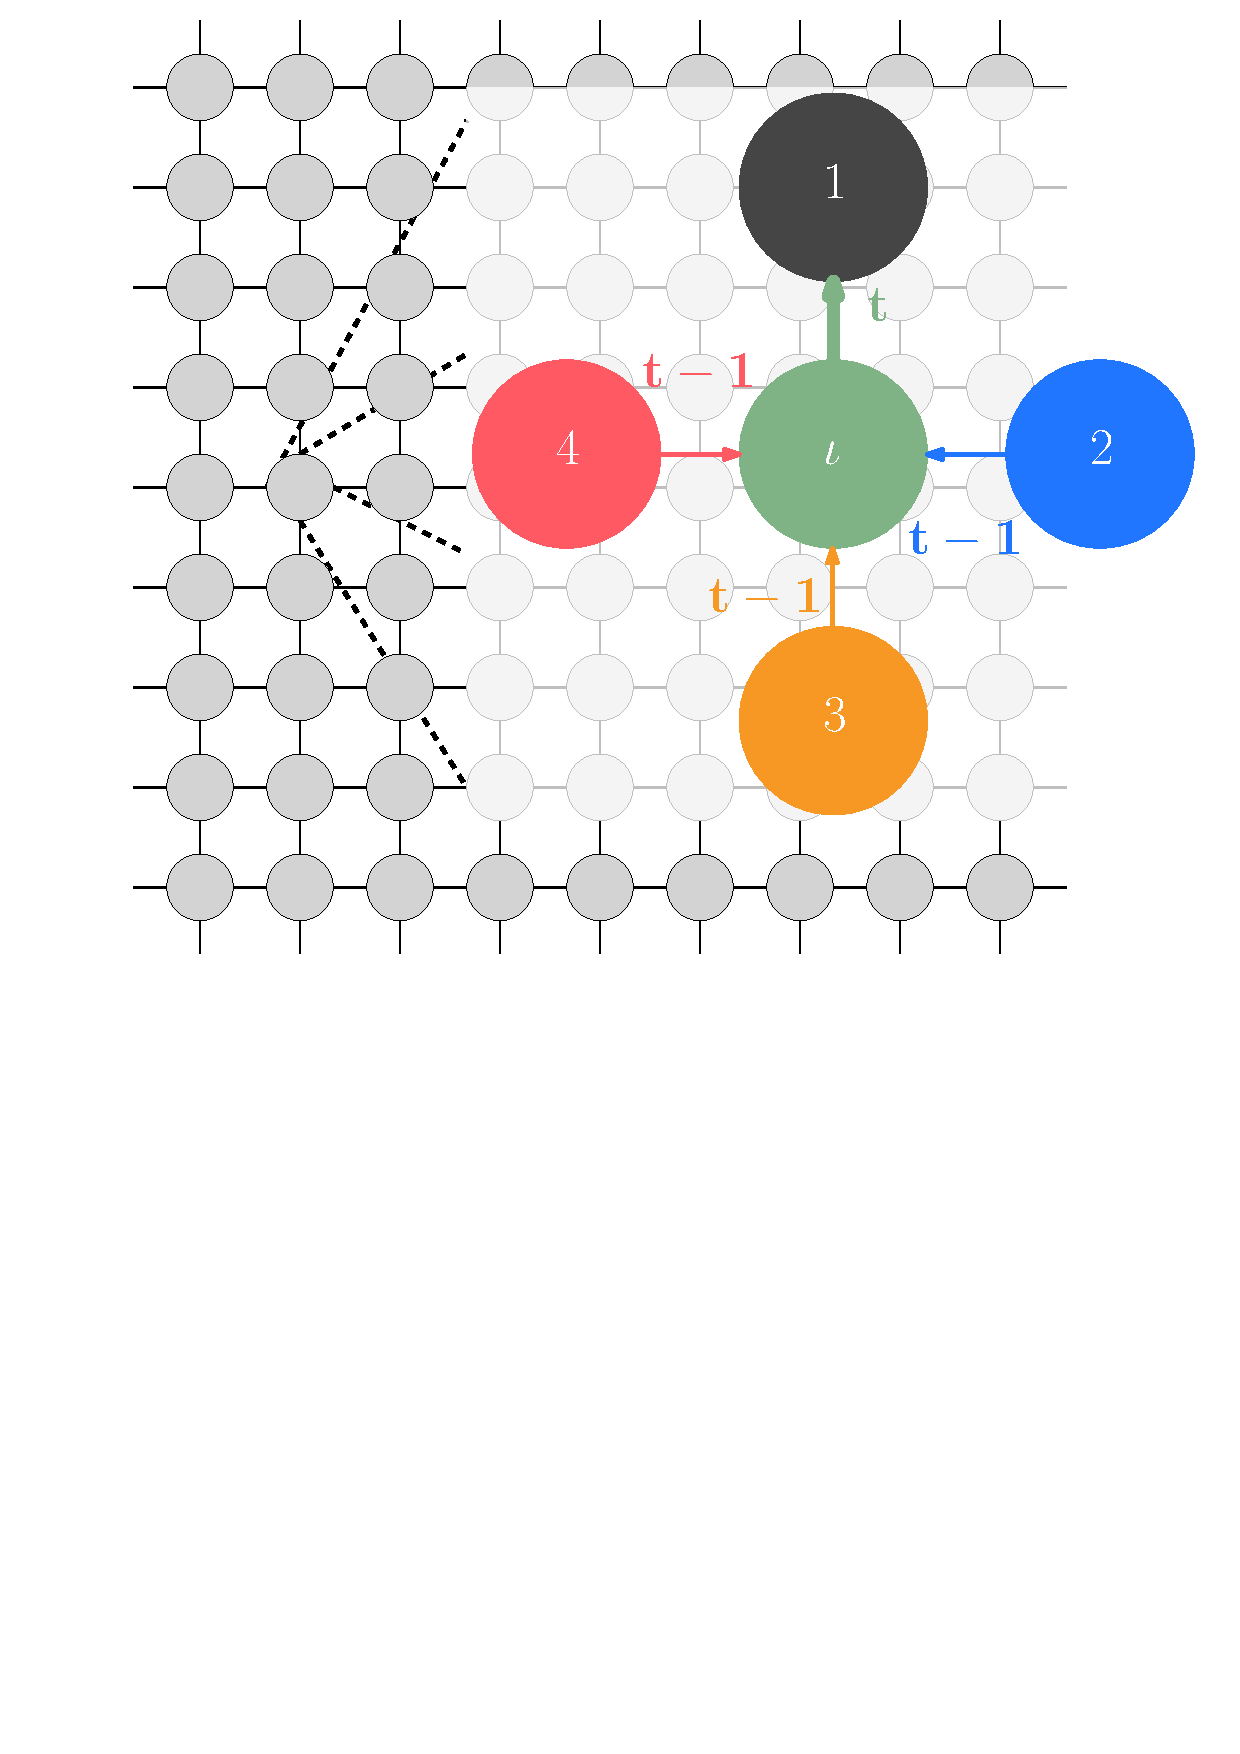
\includegraphics[keepaspectratio,width=1.0\linewidth]{chapters/nmp/images/bp_diagram_recoloured_iotacentre.pdf}
    \caption[Diagram of the central concept of \gls{fne} \glsxtrlong{nmp} on a grid]{Diagram of the central concept of \gls{fne} \gls{nmp} on a grid \cite{lbpmpsmpic}.  Each circle represents a \gls{pe}, labelled following the pattern of \cref{fig:nmp:iota_proxels_environment_oracle}.  The central \gls{pe} \(\iota\) needs to compute a new message to send at time \(t\) to \gls{pe} \(1\) above it, so it performs a computation to combine the results of the messages received from the other three neighbouring cells (\(2\), \(3\) \& \(4\)) at time \(t - 1\) (indicated by the thin and fat arrows).  The same is applied to every other neighbour, too.}
    \label{fig:nmp:gridmessaging}
\end{figure}

Conceptually, there are two distinct aspects of the \gls{nmp} process:
\begin{inparaenum}
\item the message passing itself, which occurs externally to \glspl{pe} over channels connected to other \glspl{pe}; and,
\item the data/message updates, which occur internally.
\end{inparaenum}
The focus of this \namecref{chap:nmp} is the external side, and communication with an oracle stands in for the internal computation, which is largely orthogonal to the inter-\gls{pe} communication.

There are (at least) two separate ways to model the \glspl{pe}' communication:  a \emph{\gls{gs}} system-wide view, where the states and steps taken occur across the system as a whole and every \gls{pe} carries out its operations simultaneously according to the same rules.  Or, a per-\gls{pe} view, where each \gls{pe} has its own state and advances \emph{asynchronously}\footnote{Recall from \vref{sec:back:syncasync} that the idea of asynchronicity used here follows the traditional concept from distributed computing, and so is \emph{different} to that sometimes used in other \gls{ps}.  Briefly, in the asynchronous model of distributed algorithms, external messages may take any arbitrary time (in \(\mathbb{R}\)) to reach their destinations \cite{Balanescu2011,Nicolescu2014,Lynch1996}, though internal updates are typically assumed to occur (near-)instantaneously.} without regard to others' objects, states, and rulesets.  This \namecref{chap:nmp} explores both and finds in the process that an intermediate third, \emph{\gls{ls}}, model arises naturally as a hybrid of the other two.

Modelling and implementation of \gls{nmp} proves surprisingly challenging.  The \gls{gs} form (\cref{sec:nmp:globalsync}) is reasonably simple.  It requires only nine rules, most of which have exactly one term on both the left-hand- and right-hand-sides, and none of which use \glspl{promoter} or \glspl{inhibitor} (see \cref{chap:cpsystems} for more on these concepts).

The challenge arises with the asynchronous version.  The possibility of messages from the same generation arriving at different times necessitates bookkeeping.
% It is necessary to track the sending neighbour from which each message for a given generation is received, to decide which neighbour(s) the current \gls{pe} is now ready to send a new outgoing message.
\Glspl{pe} must track from which neighbours messages have been received for a given generation, to decide to which neighbours the \gls{pe} is ready to send a new message.
This leads to inescapable complexity and the undesirable possibility of deadlock through unsuitable design.

% \Gls{nmp} shares similarities and overlaps with areas such as Cellular Automata, Gossip Protocols and Consensus Algorithms (see \eg{} [INSERT CITATIONS]). \Gls{nmp} is distinguished from these other areas in a few ways, however. Firstly, other approaches do not usually impose the ``\(n - 1\) neighbours'' condition of message updates as found in \gls{nmp}. Secondly, in other areas messaging tends to be only a part of the process, whereas in \gls{nmp} it is the heart of it. Internal computation is only performed to aggregate/average the messages received from neighbours to prepare new messages. Thirdly, in \gls{nmp} neither a global nor local consensus is sought — the closest equivalent would be the (tautological) concept of individual consensus per \gls{pe}. Rather, the result of each \gls{pe} comprises one distinct part of the final result. Lastly, often in these other areas, the neighbours are selected at random, rather than being a neighbourhood arising naturally from the structure of the modelled problem. Generalisation across these fields may be possible, but is not pursued further.
\Gls{nmp} shares similarities and overlaps with areas such as Cellular Automata, Gossip Protocols and Consensus Algorithms (see, \eg{}, \cite{Deserable2012,Hollander2015}).  \Gls{nmp} is distinguished from these other areas in a few ways, however.  Firstly, other approaches do not usually impose the ``\(n - 1\) neighbours'' condition of message updates as found in \gls{nmp}.  Secondly, in other areas messaging tends to be only a part of the process, whereas in \gls{nmp} it is the heart of it.  Internal computation is only performed to aggregate/average the messages received from neighbours to prepare new messages.  Thirdly, neither a global nor local consensus is sought in \gls{nmp} --- the closest equivalent would be the (tautological) concept of individual consensus per \gls{pe}.  Instead, the result of each \gls{pe} comprises one distinct part of the final result.  Lastly, often in these other areas, the neighbours are selected at random rather than being a neighbourhood arising naturally from the structure of the modelled problem.  Generalisation across these fields may be possible but is not pursued further.

This \namecref{chap:nmp} begins by describing a straightforward \gls{gs} \gls{nmp} system.  Then, it provides an asynchronous \gls{pe}-specific version of the same, followed by an adaptation of the asynchronous system to a \gls{ls} system. Next is a short example of a potential evolution of the asynchronous system to clarify its operation.  Lastly, this \namecref{chap:nmp} analyses the asynchronous system and reports the results of comparative computer experiments for all three systems.  The analysis proves that the asynchronous system sends precisely the same number of messages as the \gls{gs} system (one per generation per neighbour) but that the data used to compute new messages may vary slightly depending on the ordering of messages received.  Furthermore, the empirical results verify the operation of the asynchronous system and support the hypothesis that the \gls{ls} and asynchronous systems are faster than an equivalent \gls{gs} version.

\subsection{Belief Propagation}

This \namecref{chap:nmp} was originally motivated by attempts to model \emph{\gls{lbp}} for \gls{sm} (see \eg{} \cite{Blake2011,Felzenszwalb2011,Sun2003}) in \gls{cps}.  \emph{\Gls{bp}} was originally introduced to solve inference problems in AI on graphs \cite{Pearl1982} by treating the nodes as communicating objects, which passed messages backwards and forwards, updating their outgoing messages based on the incoming ones, to solve the problem.  The original formulation relied upon the graphs having a tree structure, however.  Each node would receive a message from its parent, pass that to its children, receive new messages back from the children and pass its own newly computed message back to its parent based on those received from the children.

In the case of \gls{sm}, the output is a (typically rectangular) grid representing an output image.  This means that the computation, sited on this grid, is inherently non-tree-structured.  Instead, each output node is connected to its neighbours -- usually in a \gls{fne} -- which means that messages travel in loops on the grid.  To deal with this situation, \gls{bp} was adapted to \gls{lbp}, which was first applied to \gls{sm} by \citeauthor{Sun2003} \cite{Sun2003}.  The algorithm was then significantly improved upon by \citeauthor{Felzenszwalb2006} \cite{Felzenszwalb2006}.

\Gls{nmp}, as described in this \namecref{chap:nmp}, can simulate \gls{lbp} effectively, and \cref{sec:nmp:example,sec:nmp:analysis,sec:nmp:experiments} focus on the \gls{fne}.  The main adaptation required is to replace the oracle with appropriate computations for \gls{lbp} \gls{sm}.  \Gls{nmp} can be generalised further, however, to perform other computations or use other communication arrangements besides the \gls{fne}.  While this work was originally inspired by \gls{lbp}, it is a generic framework for \emph{any} computations that may be modelled with communication on a lattice, when the outgoing message to one neighbour depends on the messages received from all other neighbours.
\section{\label{sec:nmp:systemwide}System-wide-synchronicity Messaging}

\cpresetrulenumber

This \namecref{sec:nmp:systemwide} presents the first \gls{nmp} variant, wherein the entire system evolves as one, and every \gls{pe} executes the same rule(s) simultaneously.  For the entirety of this \namecref{chap:nmp}, assume that all \glspl{pe}, channels and the oracle (\(o\)) behave correctly and follow their respective protocols, without faults, corruptions, lost messages, \etc{}  This significantly simplifies the presented systems by allowing the omission of error handling concepts and describing only the intended operation.

\begin{figure}
    \centering
    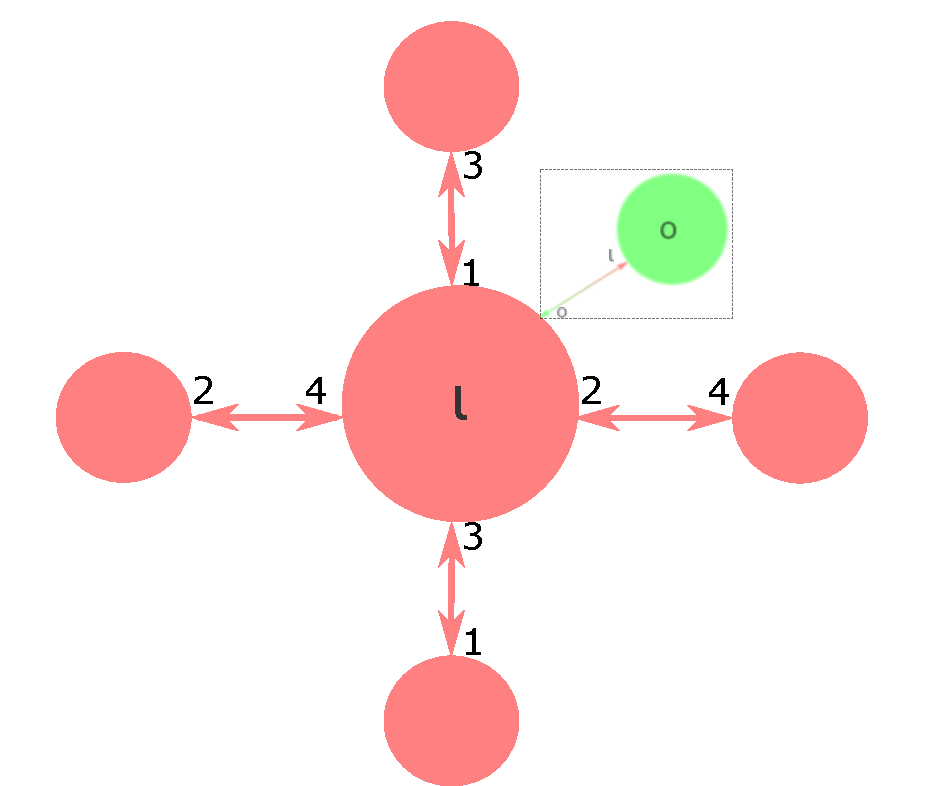
\includegraphics[width=0.9\textwidth]{chapters/nmp/images/iota_proxels_oracle_v7.pdf}
    \caption[The communication topology of a \glsxtrlong{nmp} system from the perspective of an arbitrary \glsxtrshort{pe} in a \gls{fne} arrangement]{The communication topology of the system from the perspective of an arbitrary \gls{pe} in a \gls{fne} arrangement.}
    \label{fig:nmp:iota_proxels_environment_oracle}
\end{figure}

The layout of the system, from the perspective of an arbitrary \gls{pe} in a \gls{fne}, is depicted in \cref{fig:nmp:iota_proxels_environment_oracle}.  The central circle is this \gls{pe} and is labelled with \(\iota\) to represent its ID in the overall system.  It is connected to each neighbour and the oracle by two-way channels.  The neighbours themselves are anonymous, but \(\iota\)'s end of each channel is labelled with a number from 1-4, representing the neighbours who are expected to sit above, to the right, below and to the left of the central \gls{pe}, respectively.  The oracle is smaller, blurred and surrounded with a dashed line, to reflect that it is a stand-in for an unspecified process that ordinarily would take place \emph{inside} the \gls{pe}.

In the current approach, each \gls{pe} has \emph{no} direct knowledge of its neighbouring \glspl{pe}.  Instead, it interacts with channels that connect to those neighbours; the channels interpose between the \glspl{pe}.  Furthermore, each label for a neighbour in a \gls{pe} is \emph{not} the system's ID for that neighbour, but the \gls{pe}'s label for a connecting channel endpoint.  Nevertheless, as a shortcut, \glspl{pe} will simply be referred to as communicating with their neighbours.  Messages exchanged by \glspl{pe} are termed \emph{\gls{nm} messages}, while messages exchanged with an oracle may be referred to as \emph{\gls{oq} messages}.

In the \gls{gs} version, the entire system evolves in lock-step, and thus is always in the same phase and \gls{cps} state.  The evolution follows a basic process, consisting of three conceptually distinct phases, the first two of which may be repeated.  Specifically, the system proceeds as follows (the rules are listed in \vref{ruleset:nmp:systemwide} and explained in \vref{sec:nmp:systemwide:rulesdesc}):

\begin{enumerate}
    % \item\label{enumitem:nmp:init} Initialisation (Rules \cpruleref*{rule:nmp:systemwide:recvcounter} \& \cpruleref*{rule:nmp:systemwide:recvinput})
    \item\label{enumitem:nmp:pu} \Gls{oq} (Rules \cpruleref*{rule:nmp:systemwide:loopdecrement}, \cpruleref*{rule:nmp:systemwide:sendtooracle} \& \cpruleref*{rule:nmp:systemwide:recvfromoracle})
    \item\label{enumitem:nmp:nm} \Gls{nm} (rule \cpruleref*{rule:nmp:systemwide:antiport})
    \item\label{enumitem:nmp:final} \textsf{Finalisation} (Rules \cpruleref*{rule:nmp:systemwide:loopend}, \cpruleref*{rule:nmp:systemwide:oraclefinalise} \& \cpruleref*{rule:nmp:systemwide:end})
\end{enumerate}

% This progression is depicted as a state machine in \cref{fig:nmp:systemwidestatemachine}.  State \(s_1\) covers the initialisation phase; \(s_2\) and \(s_3\) the \gls{oq} phase; \(s_4\) the \gls{nm} phase; and \(s_5\) and \(s_6\) the finalisation phase.  State \(s_7\) is the halting phase of the system's evolution.  In an application of \gls{nmp} phases \ref{enumitem:nmp:init}, \ref{enumitem:nmp:nm} and \ref{enumitem:nmp:final} will not change.  Only phase \ref{enumitem:nmp:pu} would be replaced.  The system's evolution is sketched at a high level in \cref{alg:nmp:systemwide2}.

\Cref{fig:nmp:systemwidestatemachine} depicts this progression as a state machine.  States \(s_1\) and \(s_2\) cover the \gls{oq} phase; \(s_3\) the \gls{nm} phase; and \(s_4\) and \(s_5\) the \textsf{finalisation} phase.  State \(s_6\) is the halting state of the system's evolution.  In an application of \gls{nmp} phases \ref{enumitem:nmp:nm} and \ref{enumitem:nmp:final} will not change.  Only phase \ref{enumitem:nmp:pu} is replaced.  The system's evolution is sketched at a high level in \cref{alg:nmp:systemwide2}.

The \gls{oq} phase is when each \gls{pe} performs its internal computation. As mentioned earlier, these computations are problem-dependent and thus cannot be modelled generically. Instead, this \namecref{chap:nmp} uses communication with an oracle assigned to each \gls{pe} to simulate this aspect of \gls{nmp}. The \gls{nm} phase is the main focus of this work. This is where \glspl{pe} exchange messages with their neighbours, based on data received earlier from other neighbours. The \textsf{finalisation} phase occurs after each \gls{pe} reaches a stopping point. At this point, each \gls{pe} performs a final computation to determine its output for the lattice, incorporating the latest data received from neighbours.

\begin{figure}
    \centering
    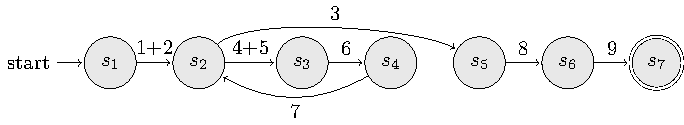
\includegraphics{chapters/nmp/images/systemwidestatemachine.pdf}
    \caption[State machine of the progression of the system-wide \glsxtrlong{nmp} \gls{cps} rules.]{State machine of the progression of the system-wide \gls{nmp} \gls{cps} rules.  The vertices are labelled with states and the arcs with the rule(s) which cause the state transitions.}
    \label{fig:nmp:systemwidestatemachine}
\end{figure}

\begin{algorithm}
\DontPrintSemicolon
\KwIn{Iteration counter \(i\) and array \(v\) of initial data}
\KwOut{Final result \(z\)}
\SetKwFor{pForEach}{parallel foreach}{do}{endfch}
\Begin{
    \tcc{\(\alpha \Leftarrow \langle \beta \rangle\) denotes receiving object \(\alpha\) on channel \(\beta\);\newline\(\gamma \Rightarrow \langle \delta \rangle\) denotes sending object \(\gamma\) on channel \(\delta\);\newline\(\epsilon \Leftrightarrow \langle \phi \rangle\) denotes antiport exchange, sending \emph{and} receiving (swapping) objects \(\epsilon\) on channel \(\phi\).}\;
    
    % \tcc{Initialisation}
    % \(i \Leftarrow \langle e \rangle\)\;
    % \lpForEach{\((x,d) \Leftarrow \langle e \rangle\)}{\(v[x] \gets d\)}\;
    
    \While{\(i > 0\)}{
        \tcc{\Glsentrylong{oq}}
        \(i \gets i - 1\)\;
        \pForEach{\(x \in \{1, 2, 3, 4\}\)}{
            \(w[x] \gets v[x]\)\;
            \(w[x] \Rightarrow \langle o \rangle\)
        }
        \lpForEach{\((x,d) \Leftarrow \langle o \rangle\)}{
            \(v[x] \gets d\)\
        }
        
        \;\tcc{\Glsentrylong{nm}}
        \lpForEach{\(x \in \{1, 2, 3, 4\}\)}{\(v[x] \Leftrightarrow \langle x \rangle\)}
    }
    \;\tcc{\textsf{Finalisation}}
    \pForEach{\(x \in \{1, 2, 3, 4\}\)}{
        \(w'[x] \gets v[x]\)\;
        \(w'[x] \Rightarrow \langle o \rangle\)
    }
    \(z \Leftarrow \langle o \rangle\)\;
    % \(z \Rightarrow \langle e \rangle\)
}
\caption[Pseudocode of the \glsxtrlong{nmp} process in the \gls{gs} system]{\label{alg:nmp:systemwide2}Pseudocode description of the process for an individual \gls{pe} in the \gls{gs} system}
\end{algorithm}

Assume before the start of the system's evolution that the correct number of \glspl{pe} are already in place, and they each contain an appropriately initialised iteration counter and their relevant channel endpoints only.  Everything else required by each \gls{pe} will be supplied by the oracle, or generated by rules during the \gls{pe}'s evolution.  The rules for the \gls{gs} system are listed in \cref{ruleset:nmp:systemwide} and explained in \cref{sec:nmp:systemwide:rulesdesc}.  This \namecref{sec:nmp:systemwide} first defines the \gls{gs} \gls{nmp} system, explains the intended operation of the \gls{ruleset}, then describes each of the ground terms used.

\subsection{System Definition}
Recall from \cref{sec:cps:formaldescriptions} that a given \gls{cps} implementation can be defined as a 6-tuple:

\cptuple{\text{NMP-GS}}{\cpset{\sigma_1, \dots, \sigma_{\text{max}}}}{A}{O}{\text{\cref{ruleset:nmp:systemwide}}}{\cpset{s_1, s_2, s_3, s_4, s_5, s_6}}{s_1}

\(T\) is a set of \glspl{tlc}, each representing a single \gls{pe}, numbered from one to the total size of the lattice.  These numbers correspond to the \(\iota\) of \cref{fig:nmp:iota_proxels_environment_oracle}.  \(A\) is the set of all terms defined in \cref{sec:nmp:systemwide:definitions}.  Each \gls{pe}'s starting multiset in \(O\) is a generation counter functor \(i\) and its set of initial data \(V\).

\subsection{\label{sec:nmp:systemwide:rulesdesc}Description of Rules}

\begin{cprulesetfloat}
    \begin{cpruleset}
        % % Receive maximum generation counter
        % \cprule[rule:nmp:systemwide:recvcounter]{s_1}{\cprecv{\cpfunc{i}{I}}{e}}{\cponce}{s_2}{\cpfunc{i}{I}}
        
        % % Receive inputs from environment
        % \cprule[rule:nmp:systemwide:recvinput]{s_1}{\cprecv{\cpvq{X}{D}}{e}}{\cpmaxpar}{s_2}{\cpvq{X}{D}}
        
        \\
        
        % Else move to finishing
        \cprule[rule:nmp:systemwide:loopend]{s_1}{i(\lambda)}{\cponce}{s_4}{}
        
        % Decrement iterator
        \cprule[rule:nmp:systemwide:loopdecrement]{s_1}{i(I\cpundig)}{\cponce}{s_2}{i(I)}
        
        % Send to oracle
        \cprule[rule:nmp:systemwide:sendtooracle]{s_1}{\cpvq{X}{D}}{\cpmaxpar}{s_2}{\cpsend{\cpvqw{X}{D}}{o}}
        
        % Receive from oracle
        \cprule[rule:nmp:systemwide:recvfromoracle]{s_2}{\cprecv{\cpvqw{X}{D}}{o}}{\cpmaxpar}{s_3}{\cpvq{X}{D}}
        
        \\
        
        % Exchange messages
        \cprule[rule:nmp:systemwide:antiport]{s_3}{\cpvq{X}{D} & & &\\ & \cpantirecv{\cpvq{\_}{D'}}{X}}{\cpmaxpar}{s_1}{\cpvq{X}{D'} &\\ & & & & \cpantisend{\cpvq{X}{D}}{X}}
        
        \\
        
        % Send to oracle (finalisation)
        \cprule[rule:nmp:systemwide:oraclefinalise]{s_4}{\cpvq{X}{D}}{\cpmaxpar}{s_5}{\cpsend{w'\perfectunary{IncreaseHeight}{(}{)}{X}\perfectunary{IncreaseHeight}{(}{)}{D}}{o}}
        
        % Oracle returns results
        \cprule[rule:nmp:systemwide:end]{s_5}{\cprecv{\cpfunc{z}{Z}}{o}}{\cpundig}{s_6}{\cpfunc{z}{Z}}
        
    \end{cpruleset}
    \caption[Complete \gls{ruleset} for \gls{gs} \glsxtrlong{nmp}]{\label{ruleset:nmp:systemwide}Complete \gls{ruleset} for \gls{gs} \gls{nmp}, using an oracle to perform update computations}
\end{cprulesetfloat}

\begin{enumerate}
    % \item Receive \(I\), the maximum generation count or the number of rounds of message passing each \gls{pe} should engage in.\footnote{In general with \gls{nmp} a fixed number of generations is not the only way to determine when \gls{nm} should cease, but other methods tend to be specific to the problem at hand.   Therefore, a generation count is the only one presented here.  It should be applicable no matter the computation performed.}
    % \item Receive from the environment \gls{nm} messages \(v(X)(D)\), being the \gls{pe}'s initial data for its neighbours.
    \item If \(i\) is empty, continue to the \textsf{finalisation} phase.
    \item Decrement \(i\) when sending \(w\) messages to the oracle for \gls{oq}.
    \item Convert the \(v\) messages into \(w\) messages and send them to the oracle to compute the new messages to send to neighbours.
    \item Receive back new \(w\) objects from the oracle and convert them to \(v\) objects.
    \item Swap \(v\) messages with each neighbour \(X\), using antiport communication (see \cref{sec:cps:antiport}).
    \item Send the \(v\) objects as \(w'\) to the oracle for \textsf{finalisation} computation.
    \item Receive the final result \(\cpfunc{z}{Z}\) from the oracle and halt.% and send it to the environment.\footnote{One might wonder why the oracle could not simply emit the final result directly into the environment.  Strictly speaking, that would be reasonable in the context of this system, but bear in mind that the oracle is simply an abstraction over an arbitrary computation, which would take place \emph{inside} the \gls{pe}.}
\end{enumerate}

\subsection{\label{sec:nmp:systemwide:definitions}Definitions of Terms}

\paragraph{Atoms}
\begin{description}
    % \cptermdef{e}{The label of the channel used to communicate with the environment.}
    \cptermdef{o}{The label of the channel used to communicate with the oracle.}
    \cptermdef{\cpempty}{The \gls{cps} `empty' atom (see \cref{sec:cps:complexsymbols,sec:cps:natnums}).}
\end{description}

\paragraph{Functors}
\begin{description}
    \cptermdef{i}{A generation counter.  Used to count the number of generations of \gls{nm} remaining before moving to the \textsf{finalisation} phase.}
    \cptermdef{v}{The \(v\) compound terms described in \cref{sec:cps:compoundterms} \emph{except} without the generation counter --- the \(i\) counter serves the same purpose for the \gls{gs} variant.  These serve as \gls{nm} messages.}
    \cptermdef{w}{The same as the \(v\) terms, but used as messages to the oracle for \gls{oq}.}
    \cptermdef{w'}{The same as the above \(w\) objects, but marked to indicate to the oracle that they are to be used for \textsf{finalisation} rather than \gls{oq}.}
    \cptermdef{z}{Final output functor.  Holds the result of the \gls{pe}’s computation.}
\end{description}

\paragraph{States}
\begin{description}
    % \cptermdef{s_1}{Beginning state.  The \glspl{pe} receive their inputs from the environment.}
    \cptermdef{s_1}{The opening \gls{oq} phase state, where data are sent to the oracle and the generation counter is decremented.}
    \cptermdef{s_2}{Data update receipt state. Updated data are received back from the oracle.}
    \cptermdef{s_3}{\Gls{nm} state.  Messages are swapped with neighbours.}
    \cptermdef{s_4}{\textsf{Finalisation} phase transition state}
    \cptermdef{s_5}{State for transmission to the oracle for the final result, and awaiting its response.}
    \cptermdef{s_6}{State for receipt of the result from the oracle and halting of evolution.}
\end{description}
\section{\label{sec:nmp:pespecific}Processing Element-specific Asynchronous Messaging}
% \cpresetrulenumber

This \lcnamecref{sec:nmp:pespecific} presents a variant of the above system where the rules are applied in a \gls{pe}-specific manner and the \glspl{pe} run \emph{asynchronously} \cite{Balanescu2011,Nicolescu2014}, so that the steps of one \gls{pe} do not necessarily occur contemporaneously with those of another.\footnote{In this form, \gls{nmp} shares some obvious similarities with \Gls{csp} (\cref{subsec:back:csp}), \Glspl{actor} (\cref{subsec:back:actors}) and \Glspl{pram} (\cref{sec:back:othermodels}).}  

\begin{anfxwarning}{Keep and modify this paragraph, or delete it?}
There is no longer a single state spanning the entire system.  Instead, each \gls{pe} has its own state dictating its operation individually.  The same conceptual phases are kept, though the \gls{oq} and \gls{nm} phases are combined because they now may occur interleaved.  During the \gls{oq} \& \gls{nm} phase, each \gls{pe} independently works through a series of \label{pg:nmp:rounds}\emph{rounds}, following the typical idea of a round in theoretical asynchronous systems:  The \gls{pe} receives one or more messages, processes the received messages and updates its internal data, then sends out new messages based on the results.
\end{anfxwarning}

The most significant change from \cref{sec:nmp:systemwide} is the use of \emph{receipt tokens} and \emph{generation counts}.  Receipt tokens show that the \gls{pe} has received a message from a particular neighbour since the last time messages were sent.  This is vital to ensure that the correct number of messages are sent, and sent only after receiving appropriate messages from other neighbours.

In the \gls{gs} system, the received messages used to update the outgoing messages could always be assumed to have been sent during the same round as each other.  This is not the case under the asynchronous system, where a message may be sent out (and thus received) as soon as the necessary input messages have been received.  This has the potential to messages being used out-of-order, where a message from what would have been an earlier `round' is re-used inappropriately.  Thus, these messages are now tagged with a round number, termed here a \emph{generation} because each outgoing message is essentially the direct progeny of the messages received at the last generation.

The other change of note is that initialisation of the \glspl{pe} also differs slightly from \cref{sec:nmp:systemwide}.  Along with the channels, each \gls{pe} also starts with an adjacency list object, \(\cpfunc{a}{A}\), which holds a copy of the atoms for each neighbour/channel.

\begin{figure}
    \centering
    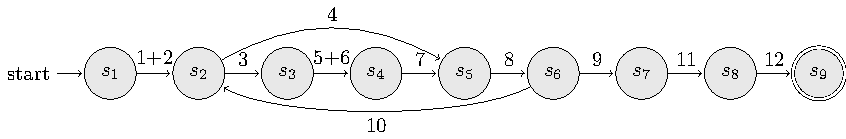
\includegraphics[width=1.0\textwidth]{chapters/nmp/images/proxelspecificstatemachine.pdf}
    \caption[State machine of the progression of the \glsxtrshort{pe}-specific \glsxtrlong{nmp} \gls{cps} rules]{State machine of the progression of the \gls{pe}-specific \gls{nmp} \gls{cps} rules.  The vertices are labelled with the states and the arcs with the rule(s) which cause that transition.}
    \label{fig:nmp:proxelspecificstatemachine}
\end{figure}

As with \cref{sec:nmp:systemwide}, this \lcnamecref{sec:nmp:pespecific} shows the progression of the system through its states in \cref{fig:nmp:proxelspecificstatemachine}.  In this system, an \gls{oq} \& \gls{nm} round can be regarded as the steps taken to proceed from state \(s_2\) until reaching \(s_2\) again.  Thus, receiving one or more messages, followed potentially by preparing and sending new messages, forms a round.  The initialisation phase is only rules \cpruleref*{rule:nmp:proxspec:initcounter} and \cpruleref*{rule:nmp:proxspec:recvinputs}.  The combined \gls{oq} and \gls{nm} phase is made up of rules \cpruleref*{rule:nmp:proxspec:makews} through \cpruleref*{rule:nmp:proxspec:recvfromneighs}, which involve the receipt of one or more messages with generation \(0 < g \leq I\) from neighbours, then preparation of new messages to send to neighbours through communicating with the oracle and forwarding the results of the oracle's computation to the relevant neighbours.  Lastly, rules \cpruleref*{rule:nmp:proxspec:finaloracle} and \cpruleref*{rule:nmp:proxspec:end} make up the finalisation phase.

\begin{algorithm}
\DontPrintSemicolon
\SetKwFunction{Uniq}{uniq}
\SetKwFunction{Perm}{permutations}
\SetKwFor{pForEach}{parallel foreach}{do}{endfch}
\SetKwBlock{Loop}{loop:}{}
\SetKw{KwOr}{or}
\SetKw{KwAnd}{and}
\SetKw{KwGoto}{goto}
\KwIn{Adjacency set \(A = \{1,2,3,4\}\)}
\KwOut{Final result, \(z\), sent to environment \(e\)}
\Begin{
    \tcc{
    \(a \Leftarrow \langle b \rangle\) denotes receiving object \(a\) on channel \(b\)\newline
    \(c \Rightarrow \langle d \rangle\) denotes sending object \(c\) on channel \(d\)
    }\;
    
    \tcc{Initialisation}
    \(R \gets \emptyset\)\;
    \(i \Leftarrow \langle e \rangle\)\;
    
    \tcc*[l]{* assume environment \(e\) sends all of these now}
    \pForEach{\((x, 0, d) \Leftarrow \langle e \rangle\)}{
        \(v[x] \gets (0,d)\)\;
        \(R \gets R \cup \{x\}\)
    }
    
    \;\tcc{\Glsentrylong{oq} \emph{and} \Glsentrylong{nm}}
    
    \Loop{
        \(W \gets \emptyset\)\;
        
        \pForEach{\((x,y,z,w) \in\) \Perm{\(A\)}}{
            \If{\(x \in R\) \KwAnd \(v[x].g < i\) \KwAnd \(v[x].g \leq v[y].g\) \KwAnd \(v[x].g \leq v[z].g\)}{
                \(W \gets W \cup (w,v[x].g+1, v[x].d \cup v[y].d \cup v[z].d))\)\label{line:nmp:rule3}
            }
        }
        
        \If{\(W \not= \emptyset\)}{
            \(W \gets\) \Uniq{\(W\)} \tcc*[l]{Multiset to set}
            \;
            \lpForEach{\((w, g, d) \in W\)}{\((w, g, d) \Rightarrow \langle o \rangle\)}
            \tcc*[l]{** assume oracle \(o\) returns all required messages}
            
            \lpForEach{\((w, g, d) \Leftarrow \langle o \rangle\)}{\((w, g, d) \Rightarrow \langle w \rangle\)}
            \(W \gets \emptyset\)
        }
        
        \(R \gets \emptyset\)\;
        \;
        \(b \gets\) \texttt{true}
        
        \lpForEach{\(x \in A\)}{\lIf*{\(v[x].g < i\)}{\(b \gets\) \texttt{false}}}
        \lIf{b}{\KwGoto break}\;
        
        \While{\(|R| = 0\)}{\label{line:nmp:recvwhile}
            \pForEach{\((x, g, d) \Leftarrow A\)}{\label{line:nmp:recvfor}
                \(v[x] \gets (g,d)\)\;
                \(R \gets R \cup \{x\}\)\;
            }
        }
        \KwGoto loop\;
    }
    \AlCapSty{\AlCapFnt break:}\;
    
    \;\tcc{Finalisation}
    
    \lpForEach{\(x \in A\)}{\(v[x] \Rightarrow \langle o \rangle\)}
    \(z \Leftarrow \langle o \rangle\)\;
    \(z \Rightarrow \langle e \rangle\)
}
\caption[Pseudocode description of the process for an individual \gls{fne} \glsxtrshort{pe} in the asynchronous system]{\label{alg:nmp:pespecific}Pseudocode description of the process for an individual \gls{fne} \gls{pe} in the asynchronous system}
\end{algorithm}

As with \cref{sec:nmp:systemwide}, this \lcnamecref{sec:nmp:pespecific} also supplies a pseudocode representation of the procedure in \cref{alg:nmp:pespecific}.  The pseudocode does not closely resemble \cref{ruleset:nmp:proxspec} in appearance.  Instead, the pseudocode is written to reflect best the meaning and intention of the rules while still relating it to the \gls{ruleset}.

An important assumption for this \gls{ruleset} is that the oracle returns all outstanding results together.  After a \gls{pe} sends one or more \gls{oq} messages to the oracle, it enters a blocking wait until it receives updated \gls{nm} messages back from the oracle.  One \gls{nm} message is expected per \gls{oq} message.  The oracle is assumed to return all these messages during one step, possibly waiting until it has finished computing new values for every message.  The same assumption is made for finalisation, and similarly, that the environment sends in all the initial messages during a single step.

In preparing the new \gls{oq} messages to go to the oracle, \cpruleref{rule:nmp:proxspec:makews} discards the information about which datum came from which neighbour (visible in \cref{line:nmp:rule3} in \cref{alg:nmp:pespecific}).  This is irrelevant for \gls{bp} \gls{sm}.  It might be relevant, however, to keep said information for a different computation.  One must bear this in mind when adapting the rules to their problem.  The changes needed are likely minor, but unexplored further here, as they are superfluous.

\subsection{System Definition}
Per the tuple definition from \cref{sec:cps:formaldescriptions}:

\cptuple{\text{NMP-Async}}{\cpset{\sigma_1, \dots, \sigma_{\text{max}}}}{A}{\cpset{\cpfunc{a}{A_t} \, | \, t \in T}}{\cref{ruleset:nmp:proxspec}}{\cpset{s_1, \dots, s_9}}{s_1}

\(T\) is a set of top-level cells, each representing a single \gls{pe}, numbered sequentially.  These numbers correspond to the \(\iota\) of \cref{fig:nmp:iota_proxels_environment_oracle}.  \(A\) is equal to the set of terms defined in \cref{sec:pespecific:definitions}.  Each \gls{pe}'s starting multiset in \(O\) is the appropriate channel endpoints and an adjacency list term \(a\), with contents \(A_t\) listing its neighbours specifically.  Every \gls{pe}'s \gls{ruleset} in \(R\) is either equal to that found in \cref{ruleset:nmp:proxspec}, or one which starts with that \gls{ruleset} as a base.  These latter \glspl{ruleset} drop terms from \cpruleref{rule:nmp:proxspec:makews} to adapt it to the relevant \gls{pe} having fewer than four neighbours (see \cref{sec:nmp:ruleslessthanfour}).

\subsection{Description of Rules}

\begin{cprulesetfloat}
    \begin{cpruleset}
    
        %%%%%%%%%%%%%  Initialisation  %%%%%%%%%%%%%
    
        % Receive inputs from environment
        \cprule[rule:nmp:proxspec:initcounter]{s_1}{\cprecv{\cpfunc{i}{I}}{e}}{\cponce}{s_2}{\cpfunc{i}{I}}
        
        \cprule[rule:nmp:proxspec:recvinputs]{s_1}{\cprecv{\cpvv{X}{\cpempty}{D}}{e}}{\cpmaxpar}{s_2}{\cpvv{X}{\cpempty}{D} & \\ & & & & \cpfunc{r}{X}}
        
        \\
        
        %%%%%%%%%%%%%  OQ & MP phase  %%%%%%%%%%%%%
        
        \cprule[rule:nmp:proxspec:makews]{s_2}{}{\cpmaxpar}{s_3}{\cpvw{W}{G\cpundig}{\cpfunc{d}{A}\,\cpfunc{d}{B}\,\cpfunc{d}{C}}}
        \cppromoter{\cpfunc{r}{X}}
        \cppromoter{\cpvv{X}{G}{A}}
        \cppromoter{\cpvv{Y}{G\cpdiscard}{B}}
        \cppromoter{\cpvv{Z}{G\cpdiscard}{C}}
        \cppromoter{\cpfunc{i}{G\cpundig\cpdiscard}}
        \cppromoter{\cpfunc{a}{\cpfunc{n}{X}\,\cpfunc{n}{Y}\,\cpfunc{n}{Z}\,\cpfunc{n}{W}}}
        
        \cprule[rule:nmp:proxspec:skiptorecv]{s_2}{}{\cponce}{s_5}{}
        
        \cprule[rule:nmp:proxspec:uniq]{s_3}{\cpvw{W}{\cpdiscard}{\cpdiscard}}{\cpmaxpar}{s_4}{}
        \cppromoter{\cpvw{W}{\cpdiscard}{\cpdiscard}}
        
        % Send to oracle
        \cprule[rule:nmp:proxspec:sendtooracle]{s_3}{\cpvw{W}{G}{D}}{\cpmaxpar}{s_4}{\cpsend{\cpvw{W}{G}{D}}{o}}
        
        % Receive from oracle & send to neighbour
        \cprule[rule:nmp:proxspec:recvfromoracle]{s_4}{\cprecv{\cpvw{W}{G}{D}}{o}}{\cpmaxpar}{s_5}{\cpsend{\cpvv{W}{G}{D}}{W}}
        
        % Clear all receipt tokens at the end of a send process
        \cprule[rule:nmp:proxspec:clearrs]{s_5}{\cpfunc{r}{\cpdiscard}}{\cpmaxpar}{s_6}{}
        
        % Transition to end if all generations complete
        \cprule[rule:nmp:proxspec:movetoend]{s_6}{}{\cponce}{s_7}{}
        \cpinhibitor{\cpvv{X}{G}{D}}
        \cppromoter{\cpfunc{i}{G\cpundig\cpdiscard}}
        
        %receive messages
        \cprule[rule:nmp:proxspec:recvfromneighs]{s_6}{\cprecv{\cpvv{\cpdiscard}{G\cpundig}{D}}{X} & & & \\ & \cpvv{X}{G}{\cpdiscard}}{\cpmaxpar}{s_2}{\cpvv{X}{G\cpundig}{D} &\\ & & & & \cpfunc{r}{X}}
        
        \\
        
        %%%%%%%%%%%%%  Finalisation %%%%%%%%%%%%%
        
        % Send to oracle
        \cprule[rule:nmp:proxspec:finaloracle]{s_7}{\cpvv{X}{G}{D}}{\cpmaxpar}{s_8}{\cpsend{w'\perfectunary{IncreaseHeight}{(}{)}{X}\perfectunary{IncreaseHeight}{(}{)}{G}\perfectunary{IncreaseHeight}{(}{)}{D}}{o}}
        
        % Oracle returns results which are immediately emitted to the environment
        \cprule[rule:nmp:proxspec:end]{s_8}{\cprecv{\cpfunc{z}{Z}}{o}}{\cpundig}{s_9}{\cpsend{\cpfunc{z}{Z}}{e}}
        
    \end{cpruleset}
    \caption[\Gls{ruleset} for the \glsfmttext{fne} \glsxtrshort{pe}-specific asynchronous \glsfmttext{nmp} system, for an inner \glsxtrshort{pe}]{\label{ruleset:nmp:proxspec}\Gls{ruleset} for the \gls{fne} \gls{pe}-specific asynchronous \gls{nmp} system, for an inner \gls{pe} (\ie{} one not on the border) and using an oracle to compute the data for outgoing messages}
\end{cprulesetfloat}

\begin{enumerate}
    \item Receive the \(\cpfunc{i}{I}\) input from the environment.
    \item Receive \(\cpvv{X}{\cpempty}{D}\) messages as inputs from the environment.
    \item Consider in turn all receipt tokens \(r\), if any (in any arbitrary order). For \(\cpfunc{r}{k_1}\) and \(\cpvv{k_1}{g_1}{\cpdiscard}\), compare generation number \(g_1\) against the generation numbers of all other current values \(\cpvv{k_j}{g_j}{\cpdiscard}, k_j \in \{k_2, k_3, k_4\} = \{1, 2, 3, 4\} \setminus \{k_1\}\). Without loss of generality, if \(g_1 \leq g_2, g_3\) \emph{and} \(g_1 < I\) (\ie{} the maximum generation count) then create a message \(w\) to send to the oracle for \gls{oq}.  This message has the data for \(k_1\), \(k_2\) and \(k_3\), which are used by the oracle in computing the new message to send to \(k_4\).  The generation count for this \(w\) message is \(g_1 + 1\).
    \item If there were no \gls{oq} messages generated by \cpruleref{rule:nmp:proxspec:makews}, then move straight to the process of testing for termination and receiving new messages.
    \item If \cpruleref{rule:nmp:proxspec:makews} resulted in the creation of more than one \gls{oq} message about a given neighbour, select one of those messages at random and delete the others.  The messages will be identical, but duplicates may arise due to the unification of different neighbours to \(Y\) and \(Z\) in \cpruleref{rule:nmp:proxspec:makews}.
    \item For each \gls{oq} message remaining after \cpruleref{rule:nmp:proxspec:uniq}, send said message to the oracle to compute the new corresponding outgoing \gls{nm} message.
    \item Forward newly prepared \gls{nm} messages \(v\) from the oracle to the relevant neighbour.
    \item Delete all extant receipt tokens after completing the relevant \gls{oq} \& \gls{nm} phase.
    \item If messages with a generation count equal to \(I\) have been received from every neighbour, transition to the finalisation phase.
    \item Receive a message \(\cpvv{\cpdiscard}{G}{D}\) from neighbour \(X\) and replace the current \(v\) object for \(X\) with it.  The neighbour label contained inside the message is overwritten with the current \gls{pe}'s label for the receiving channel.  Create a receipt token \(\cpfunc{r}{X}\).
    \item Send all the \gls{pe}'s \(v\) messages to the oracle, for the oracle to compute the final output for the \gls{pe}.
    \item Receive the computed final result from the oracle and send it to the environment.
\end{enumerate}

\subsection{\label{sec:pespecific:definitions}Definitions of Terms}

\paragraph{Atoms}
The same as in \cref{sec:nmp:systemwide}.

\paragraph{Functors}
\begin{description}
    \cptermdef{a}{Adjacency set.  Lists the neighbours of the \gls{pe} as a set of \(n\) functors.}
    \cptermdef{i}{Maximum generations counter.  Used slightly differently to \cref{sec:nmp:systemwide}.}
    \cptermdef{n}{Neighbourhood functor.  Stores the label for one of the channels/neighbours to which the current \gls{pe} is connected.}
    \cptermdef{r}{Receipt token, showing that a message was recently received from neighbour \(X\).}
    \cptermdef{v}{Serves as both the internal data stores and \gls{nm} messages of the system.  These are the \(v\) compound terms described in \cref{sec:cps:compoundterms}.}
    \cptermdef{w}{Identical in most respects to \(v\) functors, except used for messaging with the oracle instead of neighbouring \gls{pe}.  That is, these are \gls{oq}, rather than \gls{nm}, messages.}
    \cptermdef{w'}{Identical to \(w\), except marked to indicate to the oracle that the messages sent are to be used for finalisation computations instead of \gls{oq}.}
    \cptermdef{z}{Identical to the \(z\) in \cref{sec:nmp:systemwide}.}
\end{description}

\paragraph{States}
\begin{description}
    \cptermdef{s_1}{Environmental inputs receipt state.}
    \cptermdef{s_2}{Messaging round starting state.  If it is appropriate for the \gls{pe} to send new messages to its neighbours, then \gls{oq} messages are prepared and the sending process continues.  Otherwise, return to receiving once again.}
    \cptermdef{s_3}{Message send phase, part 1.  Drop any duplicate \gls{oq} messages referring to the same neighbour.   Send \gls{oq} messages to compute new outgoing \gls{nm} messages.}
    \cptermdef{s_4}{Receive the new \gls{nm} messages computed by the oracle, and forward them to the appropriate neighbour(s).}
    \cptermdef{s_5}{Receipt token deletion state.  Unconditionally delete all receipt tokens present.}
    \cptermdef{s_6}{Message receipt state.  When there are no messages to send, the \gls{pe} performs a `blocking' receipt (see \cref{sec:cps:blocking}) in this state until one or more of its neighbours send messages on the connecting channels.}
    \cptermdef{s_7}{Equivalent to state \(s_5\) in \cref{sec:nmp:systemwide}.}
    \cptermdef{s_8}{Equivalent to state \(s_6\) in \cref{sec:nmp:systemwide}.}
    \cptermdef{s_9}{Equivalent to state \(s_7\) in \cref{sec:nmp:systemwide}.}
\end{description}

\subsection{\label{sec:nmp:ruleslessthanfour}Rules for \glsfmtname{fne} Proxels with Fewer Than Four Neighbours}

\Cref{ruleset:nmp:proxspec} considers only the case where a \gls{pe} has exactly four neighbours.  This does not work correctly for those \glspl{pe} with three neighbours (\ie{} on the grid border, but not in a corner) or two neighbours (\ie{} in a grid corner).  The only adjustment necessary to handle these edge cases is to change the number of neighbours considered, specifically in \cpruleref{rule:nmp:proxspec:makews}.

These alternative rules are listed in \cref{ruleset:nmp:3alts} as {\cpruleref{rule:nmp:proxspec:makews}a} and {\cpruleref{rule:nmp:proxspec:makews}b} for the border and corner cases, respectively.  Assume henceforth that any \gls{nmp} system is constructed to handle the finite boundaries of the grid correctly by replacing the usual \cpruleref{rule:nmp:proxspec:makews} with the suitable alternative for edge \glspl{pe}.  \Cref{sec:nmp:example} uses rule {\cpruleref{rule:nmp:proxspec:makews}a} to simplify and shorten the example without neglecting the essential details.

\begin{cprulesetfloat}
    \begin{cpruleset}
        \cprulecustnum{s_2}{}{\cpmaxpar}{s_3}{\cpvw{W}{G\cpundig}{\cpfunc{d}{A} \, \cpfunc{d}{B}}}{\cpruleref*{rule:nmp:proxspec:makews}a}
        \cppromoter{\cpfunc{r}{X}}
        \cppromoter{\cpvv{X}{G}{A}}
        \cppromoter{\cpvv{Y}{G\cpdiscard}{B}}
        \cppromoter{\cpfunc{i}{G\cpundig\cpdiscard}}
        \cppromoter{\cpfunc{a}{\cpfunc{n}{X} \, \cpfunc{n}{Y} \, \cpfunc{n}{W}}}
        
        \\
        
        \cprulecustnum{s_2}{}{\cpmaxpar}{s_3}{\cpvw{W}{G\cpundig}{\cpfunc{d}{A}}}{\cpruleref*{rule:nmp:proxspec:makews}b}
        \cppromoter{\cpfunc{r}{X}}
        \cppromoter{\cpvv{X}{G}{A}}
        \cppromoter{\cpfunc{i}{G\cpundig\cpdiscard}}
        \cppromoter{\cpfunc{a}{\cpfunc{n}{X} \, \cpfunc{n}{W}}}
        
    \end{cpruleset}
    \caption[Alternative forms of \cref{ruleset:nmp:proxspec}'s rule 3]{\label{ruleset:nmp:3alts}Alternative forms of \cref{ruleset:nmp:proxspec}'s \cpruleref{rule:nmp:proxspec:makews} for \glspl{pe} on the border of a grid or in the corner of a grid, respectively}
\end{cprulesetfloat}

A strength of \gls{cps} in \cref{chap:tsp,chap:gcol} was the fact that one rule system applies to all possible problems.  Modifying the rules to fit the problem weakens that strength.  An alternative is the use of `dummy' or `sentinel' \glspl{pe} with special rules outside the grid connected to the corner and border \glspl{pe}.  The specifics of the special rules are situation-dependent and so unexplored here.

\subsection{Traces}

% A \emph{trace} is a sequence of \emph{snapshots}, connected by arrows \tarr{}, describing the evolution of message generation numbers. A snapshot is an \(m\)-tuple, where \(m\) is the number of neighbours for the relevant \gls{pe}:  \((g_1, g_2, g_3, g_4)\) for a \gls{fne}, where \(g_k\) is the generation number of the last message \(\cpvv{k}{g_k}{\cpdiscard}\) received from neighbour \(k\).  The period between snapshots is a \emph{round}, as described on page~\pageref{pg:nmp:rounds}.  The initialisation and finalisation phases may be included in a trace as single rounds along with \gls{oq} \& \gls{nm}.

A \emph{trace} is a sequence of \emph{snapshots}, connected by arrows \tarr{}, describing the evolution of message generation numbers. A snapshot is an \(m\)-tuple, where \(m\) is the number of neighbours for the relevant \gls{pe}:  \((g_1, g_2, g_3, g_4)\) for a \gls{fne}, where \(g_k\) is the generation number of the last message \(\cpvv{k}{g_k}{\cpdiscard}\) received from neighbour \(k\).  The period between snapshots is a \emph{round}, as described in \cref{sec:back:syncasync}.  The initialisation and finalisation phases may be included in a trace as single rounds along with \gls{oq} \& \gls{nm}.

By convention, for a \gls{fne} \gls{pe}, the entries in a snapshot are written clockwise starting from the top.  That is, the first entry is the neighbour above the current \gls{pe}, the second entry the neighbour to the right, \etc{}  If there is no message pertaining to a given neighbour present inside the relevant \gls{pe}/top-level cell, `--' is used in place of the corresponding generation number.

Optionally, snapshots may be decorated further with 
{\renewcommand{\theenumi}{\alph{enumi}}
\begin{enumerate}
    \item A round number, \(h\): \trace{\(g_1\)}{\(g_2\)}{\(g_3\)}{\(g_4\)}\(_h\).
    \item Each component \(g_k\) can be followed by a question mark \(?\), showing that a message was just received from that neighbour at the start of the current round.
    \item Each component \(g_k?\) can be further followed by one or more stars \(*\), one for each message sent because of the corresponding incoming message.
\end{enumerate}}

Contemporaneous receipts from different neighbours may lead to the same outgoing message(s).  As a convention, the left-most \(g_k?\) which triggers the outgoing message will be marked with the corresponding \(*\).

For example, a snapshot where the latest iterations received from the first through fourth neighbours are 2, 3, 1 and 2, respectively, and a message has just been received from neighbour four, would look like:  \trace{2}{3}{1}{2?*}.  A trace documenting this could look like \tracen{2}{3}{1}{1} \tarr{} \tracen{2}{3}{1}{2?*}.
\section{\label{sec:nmp:localsync}Alternative `\glsfmtname{ls}' Rules}
It is possible to define a \gls{ruleset} where each \gls{pe} is \emph{\gls{ls}}.  A \gls{ls} \gls{pe} is one that waits until it has received \emph{all} of its expected incoming messages for a given generation before continuing.  The difference between the \gls{ls} and asynchronous \gls{nmp} processes is that a \gls{pe} working in the asynchronous style will start a new round after receiving \emph{any} message(s) --- it only needs to receive one before starting a new round.  Whereas, a \gls{ls} \gls{pe} will remain (effectively) in a blocking wait until it has received messages for the next generation from \emph{all} of its neighbours, however long that takes.

To go from the asynchronous \gls{ruleset} to a \gls{ls} one requires only changing \cref{ruleset:nmp:proxspec}'s \cpruleref{rule:nmp:proxspec:recvfromneighs}, splitting it into two related rules, as shown in \cref{ruleset:nmp:localsync}.  Combined, the two in effect serve to change the stopping condition of the message receipt process.  Where the asynchronous rules merely block until a message arrives over \emph{any} channel, the \gls{ls} rules block until exactly one message has been received from \emph{every} neighbour.  \cpRuleref[a]{rule:nmp:proxspec:recvfromneighs} terminates the blocking wait once all messages are received.  \cpRuleref[b]{rule:nmp:proxspec:recvfromneighs} continues message receipt, but prevents the receipt of more than one message from a neighbour during the same round.

Similarly, the pseudocode from \cref{alg:nmp:pespecific} requires only two changes, on \cref{line:nmp:recvwhile,line:nmp:recvfor}.  On \cref{line:nmp:recvwhile}, the condition for the \texttt{while} loop changes from \(|R| = 0\) to \(R \not= A\), reflecting that the \gls{pe} now waits until it has received a message from \emph{every} neighbour, rather than one or more.  On \cref{line:nmp:recvfor}, the set from which the \gls{pe} receives changes from \(A\) to \(A \setminus R\), reflecting that only a single message should be received from each neighbour during the current round of \gls{nmp}.

\begin{cprulesetfloat}
    \begin{cpruleset}
    
        \cprulecustnum{s_6}{}{1}{s_2}{}{10a}
        \cppromoter{\cpfunc{r}{X} \; \cpfunc{r}{Y} \; \cpfunc{r}{Z} \; \cpfunc{r}{W}}
        \cppromoter{\cpfunc{a}{\cpfunc{n}{X}\,\cpfunc{n}{Y}\,\cpfunc{n}{W}}}
        
        \cprulecustnum{s_6}{\cprecv{\cpvv{\_}{G\cpundig}{D}}{X} & & & \\ & \cpvv{X}{G}{\_}}{+}{s_6}{\cpvv{X}{G\cpundig}{D} &\\ & & & & \cpfunc{r}{X}}{10b}
        \cpinhibitor{\cpfunc{r}{X}}
        
    \end{cpruleset}
    \caption[Alternative forms of \cref{ruleset:nmp:proxspec}'s Rule 10]{\label{ruleset:nmp:localsync}Alternative forms of \cref{ruleset:nmp:proxspec}'s \cpruleref{rule:nmp:proxspec:recvfromneighs} for a \gls{pe} operating in a \gls{ls}, rather than asynchronous, fashion.}
\end{cprulesetfloat}

In the context of \gls{cps}, there is no meaningful difference in the end result of the \gls{gs} \gls{ruleset} of \cref{sec:nmp:systemwide} and the \gls{ls} rules.  In practice with implementations on typical electronic computers, however, there likely is a difference in total running times due to eliminating the need to synchronise across the entire lattice.  Each \gls{pe} now needs to wait only for its slowest neighbour during a given round, rather than the entire lattice waiting for the overall slowest \gls{pe}.  The comparative performance of all three of the `globally' synchronous, \gls{ls}, and asynchronous rules, is investigated further in \cref{sec:nmp:timingexp}.

The \gls{ls} rules necessarily work similarly to the asynchronous rules regarding receipts.  In both cases, the next messages due from every neighbour may not arrive during the same rule execution step.  The only real difference is that the \gls{ls} version loops until it has received a message for the next generation from every neighbour, instead of moving on after receiving any message.  Sending may differ between the two, however.  In the case of the asynchronous system, it is possible for a \gls{pe} not to have received all the messages required to compute the new outgoing message for a given neighbour at the start of a round.  This is untrue for the \gls{ls} version, which by its nature guarantees that a \gls{pe} has sufficient information for every outgoing message at the start of the next round.  The rules for the \gls{ls} version could thus be simplified so that the sending process much more closely matches the \gls{gs} version if desired.


\section{\label{sec:nmp:example}Asynchronous system example}
\newcommand*{\obinnod}[1]{Objects inside node 1 at the end of round #1}
\newcommand*{\obinrul}[2]{Objects inside node 1 after application of rule#1 during round #2}

This section steps through a simple example of the evolution of \cref{sec:nmp:pespecific}'s asynchronous variant of \gls{nmp}.  The grid in question is found in \cref{fig:nmp:basicgrid}, and this example focuses on the node marked ``1''.  For simplicity, and to demonstrate the broader application of the ruleset, we choose to focus on a border point in the grid, i.e., a \gls{pe} with a \emph{three}-neighbourhood.  Two generations of \gls{nm} are shown (i.e., the maximum generation count is 2: \(\cpfunc{i}{2}\)) for demonstration purposes.  Node 1 starts in state \(s_1\) and its adjacency list object is \(\cpfunc{a}{\cpfunc{n}{2} \; \cpfunc{n}{3} \;\cpfunc{n}{4}}\).

\begin{figure}
    \centering
    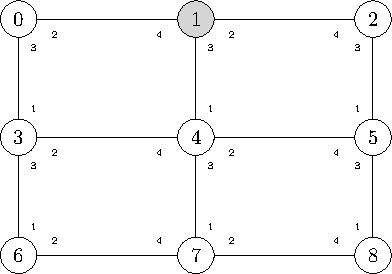
\includegraphics[keepaspectratio,width=0.7\textwidth,height=0.3\textheight]{chapters/nmp/images/3by3gridgraph.pdf}
    \caption[Basic 3×3 grid graph used for the example]{Basic 3×3 grid graph used for the example.  This example will focus on the perspective of node 1.  Other nodes are assumed to work equivalently, but their evolution is not discussed.  Nodes are labelled internally with their ID in the system (\(\iota\) in \cref{fig:nmp:iota_proxels_environment_oracle}), and each intermediary channel with the identity assigned to it by the nearby \gls{pe}.}
    \label{fig:nmp:basicgrid}
\end{figure}

Embodying the unknown processes of the oracle, the data for the received \(v\) terms have been randomly generated for this example and have no particular significance.

To supply a partial demonstration of the expected operation of the rule(s) which would replace the oracle, we compute the contents of outgoing messages according to the following simple rule: \cpruleinline{\cprulenonum{s_4}{\cprecv{\cpvw{W}{G}{\cpfunc{d}{A} \; \cpfunc{d}{B}}}{\iota}}{1}{s_5}{\cpsend{\cpvw{W}{G}{AB}}{\iota}}}  This rule merely sums the data received, and returns the newly computed outgoing message to the relevant node.

\setcounter{traces}{-1}

The total trace for this example is: \tracn{{\label{trace:nmp:0}}--}{--}{--} \tarr{} \tracn{\label{trace:nmp:1}0?*}{0?*}{0?*} \tarr{} \tracn{\label{trace:nmp:2}1?*}{0}{1?} \tarr{} \tracn{\label{trace:nmp:3}1}{0}{2?} \tarr{} \tracn{\label{trace:nmp:4}2?}{1?**}{2} \tarr{} \tracn{\label{trace:nmp:5}2}{2?}{2} \tarr{} \tracn{\label{trace:nmp:6}--}{--}{--}.  Each round number of the trace corresponds to the same row in \cref{tab:nmp:exampleobjects}, reflecting the state of node 1 at the end of that round.  Where the contents of a functor change, the functor and its changed contents are written in boldface to highlight the modifications.

\begin{table}
\setlength\extrarowheight{1ex}
\centering
\begin{tabular}{|l|l|}
\hline
\textbf{Round number} & \textbf{Objects in Node 1} \\ \hline
0 & \(\cpfunc{a}{\cpfunc{n}{2} \, \cpfunc{n}{3} \, \cpfunc{n}{4}}\) \\ \hline
1 & \(\cpfunc{a}{\cpfunc{n}{2} \, \cpfunc{n}{3} \, \cpfunc{n}{4}} \quad \cpfunc{\mathbf{i}}{\mathbf{2}} \quad \cpvvbf{\mathbf{2}}{\mathbf{0}}{\mathbf{1}} \; \cpvvbf{\mathbf{3}}{\mathbf{0}}{\mathbf{4}} \; \cpvvbf{\mathbf{4}}{\mathbf{0}}{\mathbf{7}}\) \\ \hline
2 & \(\cpfunc{a}{\cpfunc{n}{2} \, \cpfunc{n}{3} \, \cpfunc{n}{4}} \quad \cpfunc{i}{2} \quad \cpvvbf{2}{\mathbf{1}}{\mathbf{9}} \; \cpvv{3}{0}{4} \; \cpvvbf{4}{\mathbf{1}}{\mathbf{5}}\)  \\ \hline
3 & \(\cpfunc{a}{\cpfunc{n}{2} \, \cpfunc{n}{3} \, \cpfunc{n}{4}} \quad \cpfunc{i}{2} \quad \cpvv{2}{1}{9} \; \cpvv{3}{0}{4} \; \cpvvbf{4}{\mathbf{2}}{\mathbf{2}}\)  \\ \hline
4 & \(\cpfunc{a}{\cpfunc{n}{2} \, \cpfunc{n}{3} \, \cpfunc{n}{4}} \quad \cpfunc{i}{2} \quad \cpvvbf{2}{\mathbf{2}}{\mathbf{8}} \; \cpvvbf{3}{\mathbf{1}}{\mathbf{3}} \; \cpvv{4}{2}{2}\)  \\ \hline
5 & \(\cpfunc{a}{\cpfunc{n}{2} \, \cpfunc{n}{3} \, \cpfunc{n}{4}} \quad \cpfunc{i}{2} \quad \cpvv{2}{2}{8} \; \cpvvbf{3}{\mathbf{2}}{\mathbf{7}} \; \cpvv{4}{2}{2}\)  \\ \hline
6 & \(\cpfunc{a}{\cpfunc{n}{2} \, \cpfunc{n}{3} \, \cpfunc{n}{4}} \quad \cpfunc{i}{2}\)  \\ \hline
\end{tabular}
\caption[Objects present inside Node 1 at the end of each round]{Objects present inside Node 1 at the end of each round in the example}
\label{tab:nmp:exampleobjects}
\end{table}

\paragraph{Round One}
This round is where node 1 receives its inputs from the environment by rules 1 and 2.  The maximum message generations counter, and the messages with the initial data for the \gls{pe} come through the channel connected to the environment.  Node 1 starts this round holding only its adjacency list, in this case \(\cpfunc{a}{\cpfunc{n}{2} \, \cpfunc{n}{3} \, \cpfunc{n}{4}}\).

The receipt of messages for all three neighbours causes rule 3 to apply and node 1 to enter the sending cycle.  Two new \gls{oq} \(w\) messages are generated relating to each neighbour (because the other two neighbours will take the place of \(Y\) in applications of rule 3a --- recall that there is no \(Z\) in the rule for this node, as it only has three neighbours).  Rule 5 eliminates these duplicates, however, leaving one copy of each message for rule 6 to send to the oracle.  These outgoing messages to the oracle are \(\cpvw{2}{1}{\cpfunc{d}{4} \, \cpfunc{d}{7}}\), \(\cpvw{3}{1}{\cpfunc{d}{1} \, \cpfunc{d}{7}}\) and \(\cpvw{4}{1}{\cpfunc{d}{1} \, \cpfunc{d}{4}}\) for neighbours 2, 3, and 4, respectively.

Node 1 then enters a `blocking wait' (see \cref{sec:cps:blocking}) and remains inactive until the oracle returns the new \gls{nm} messages to send to each neighbour.  Rule 7 sees node 1 receive those messages and then immediately forward them to the neighbours.  The messages are not stored inside node 1 at the end of a step.  Following the example oracle rule described above, the messages sent are \(\cpvv{2}{1}{11}\), \(\cpvv{3}{1}{8}\) and \(\cpvv{4}{1}{5}\) for neighbours 2, 3, and 4, respectively.

The application of rule 7 brings the sending cycle to a close, and node 1 moves to state \(s_5\).  In this state, rule 8 clears away any receipt tokens present in the \gls{pe} and then moves to the termination check of rule 9.  At this point, none of the \(v\) messages hold generation counters equal to the maximum generation count, and so processing will continue.  Finally, node 1 proceeds with another blocking wait, until messages arrive from one or more of its neighbours.

\paragraph{Round Two}
The second round proceeds similarly to the first, but with two key differences.  Firstly, the incoming messages are received from neighbouring \glspl{pe} via the channels connecting node 1 to them.  Secondly, messages are received only from neighbours 2 and 4.  This generates receipt tokens for those neighbours and sees node 1 enter a new sending cycle.

The presence of receipt tokens for both neighbours 2 and 4 leads to the creation of two duplicate \(w\) \gls{oq} messages about neighbour 3.  In effect, 1 and 3 swap roles as \(X\) and \(Y\) in rule 3.  Again, rule 5 eliminates the duplicate, and the single message \(\cpvw{3}{2}{\cpfunc{d}{9} \, \cpfunc{d}{5}}\) is sent to the oracle with rule 6.  In turn, by rule 7, node 1 receives back \(\cpvv{3}{2}{14}\) and forwards it to neighbour 3, completing the sending cycle.  This is also the final message sent to neighbour 3, given that the maximum generation count for this system is two.

As before, node 1 moves from sending to clearing receipt tokens, checking whether it has completed \gls{nm}, and finally becomes quiescent once more, awaiting further messages from neighbours.

\paragraph{Round Three}
Round three begins with receiving a single message, the final message to be received from neighbour 4.  Unlike the earlier rounds, no new messages are sent out due to said receipt.  Neighbour 4 was already one of the neighbours with the highest generation count amongst the messages stored in node 1, and so while it can serve as \(X\) in rule 3, neither of neighbours 2 or 3 can serve as \(Y\) because their generation counts are lower than neighbour 4's.

The fact that rule 3 does \emph{not} apply means that rule 4 \emph{is} applied --- for the first time in this system's evolution.  Rule 4 unconditionally transitions node 1 back to removing all extant receipt tokens, before progressing to the termination check and then returning to awaiting new messages.

\paragraph{Round Four}
This time, neighbour 2 sends its final message, and neighbour 3, at last, sends its first message.  The receipt from neighbour 3 leads to two new single instances of messages relating to neighbours 2 and 4.  The receipt from neighbour 2 could ordinarily lead to another message to be sent to neighbour 3, as it would pair up with neighbour 4 to act as \(X\) and \(Y\), respectively, in rule 3.  This does not occur, however, as neighbour 2 (and 3) has reached the maximum generation count, so rule 3 is no longer applicable for it.

The messages to go to the oracle due to the receipt from neighbour 3 are \(\cpvw{2}{2}{\cpfunc{d}{3} \, \cpfunc{d}{2}}\) and \(\cpvw{4}{2}{\cpfunc{d}{8} \, \cpfunc{d}{3}}\).  Thus, the messages returned by the oracle and sent to neighbour 2 and are \(\cpvv{2}{2}{5}\) and \(\cpvv{4}{2}{11}\).  These are, the last two messages to be sent by node 1 to its neighbours.

\paragraph{Round Five}
Only one more message is still to be received, from neighbour 3 specifically. Node 1 will wait until said message is received, but at that point, all message generation counters will be equal to the maximum, and thus no further messages will be sent out to the neighbours.

Following the application of rule 10 to receive the final message from neighbour 3, node 1 returns to state \(s_2\) and the rules are again explored in top-down order.  This time, rule 3 is inapplicable, so rule 4 is applied, transitioning node 1 to state \(s_5\).  Rule 4 is the only rule applied at this step because it is the only rule which moves from state \(s_2\) to state \(s_5\).  Next, rule 8 deletes the last receipt token.  Again, rule 8 is the only rule applied because it is the only one to feature its state transitions.  Finally, without any \(v\) messages with a generation count below the maximum present in the \gls{pe}, by rule 9, node 1 moves to state \(s_7\) and the finalisation phase.

\paragraph{Round Six}
Round six is the final round of the evolution of the system, for node 1 at least.  With node 1 in state \(s_7\), the only applicable rule is rule 11.  The effect of rule 11 is to send every \(v\) message stored in node 1 to the oracle, renaming them to \(w'\) messages so that the oracle recognises them as finalisation messages rather than \gls{oq} messages for \gls{nm} purposes.

Eventually, the oracle will return the final result message, with the contained datum computed by some means from the messages the oracle received from node 1.  That message is immediately forwarded back to the environment, and evolution of node 1 halts.  Once all other nodes have halted, evolution of the system will have terminated.
\section{\label{sec:nmp:analysis}Asynchronous System Analysis}

This \lcnamecref{sec:nmp:analysis} examines and analyses the asynchronous \gls{pe}-specific system of \cref{sec:nmp:pespecific}.  Firstly, it describes and proves several properties about the system, in particular, that the asynchronous system exchanges precisely the same number of \gls{nm} messages as the \gls{gs} system of \cref{sec:nmp:systemwide}.  Then, it states three conjectures about the system, yet to be proven or disproven mathematically, before examining the asynchronous system's complexity from the standpoint of the rules and symbols used.  Lastly, the \lcnamecref{sec:nmp:analysis} discusses some visualisations of the propagation of ``influence'' from one \gls{pe} in a \gls{fne} grid to others, over multiple steps.

Recall that the fundamental difference in behaviour between the \gls{gs}, \gls{ls} and asynchronous variants is the timing of when they send out new messages relating to when they have received messages for the previous generation.  Under the \gls{gs} approach, \emph{every} \gls{pe} waits until every other \gls{pe} has received all incoming messages before progressing.  Following the \gls{ls} methodology, each \gls{pe} waits until it has received all of its due incoming messages before proceeding, \emph{but without regard} to any other \gls{pe}.  Lastly, for the asynchronous variant, a \gls{pe} waits only until it has received the \(n - 1\) required messages from the other neighbours of generation \(g\) before sending the appropriate generation \(g + 1\) message to the \(n^\text{th}\) neighbour.

\subsection{\label{sec:nmp:msgprops}Messaging Properties and Behaviours}

Consider a cell (\gls{pe}) $\pi_0$ in the asynchronous framework of \cref{sec:nmp:pespecific},
where the maximum generation count is $I$, set by the environment via $\cpfunc{i}{I}$.
Without loss of generality, 
we consider only a \gls{fne} system and
assume that $\pi_0$ is a non-border/non-corner cell with four neighbours, 
$\pi_k$, accessible via channels labelled by $k \in \{ 1, 2, 3, 4 \}$. 

\begin{lemma}\label{lemma:nmp:-0}
    For any $k \in \{ 1, 2, 3, 4 \}$, after each round except the last,
    cell $\pi_0$ contains exactly one $k$-tagged value $\cpvv{k}{\cpdiscard}{\cpdiscard}$, 
    which is accepted from channel $k$ 
    --- except the first round, when that value $v$ comes from the environment channel $e$.
\end{lemma}

\begin{proof}
    By \cpruleref{rule:nmp:proxspec:recvinputs}, cell $\pi_0$ starts by accepting a value $\cpvv{k}{0}{\cpdiscard}$, from the environment channel $e$.
    \cpRuleref{rule:nmp:proxspec:recvfromneighs} gives the only possibility of obtaining another $k$-tagged value, by replacing the current value $v$ with another value $v'$, accepted from channel $k$.
\end{proof}

\begin{remark}
    In fact, \cref{lemma:nmp:-0} holds practically at all times, not just at the end of each round.  The only exceptions are: before the start of the system's evolution and application of \cpruleref{rule:nmp:proxspec:recvinputs}; and after the start of the finalisation phase, specifically after applying \cpruleref{rule:nmp:proxspec:finaloracle}.
\end{remark}

\begin{lemma}\label{lemma:nmp:-1}
    For any $k \in \{ 1, 2, 3, 4 \}$, the time sequence of generation numbers $g \geq 0$ of accepted values $\cpvv{k}{g}{\cpdiscard}$ forms an arithmetic progression with step size one.
\end{lemma}

\begin{proof}
    Proof by induction. Cell $\pi_0$ starts with value $\cpvv{k}{0}{\cpdiscard}$, received via the environment channel $e$.
    Assume that this hypothesis holds for a given $g \geq 0$, appearing as a generation number in value $\cpvv{k}{g}{\cpdiscard}$. \cpRuleref{rule:nmp:proxspec:recvfromneighs} gives the only possibility of changing this number, by replacing the current value with another $v$ value, where the generation number is strictly greater by one, 
    $\cpvv{k}{g+1}{\cpdiscard}$.
\end{proof}

\begin{remark}\label{remark:nmp:-1}
The conclusion of \cref{lemma:nmp:-1} will hold even in the hypothetical case that cell $\pi_k$ would be allowed to send multiple copies of the same message $v$. 
Only the first received copy will be accepted, and the rest will be ignored,
courtesy of \cpruleref{rule:nmp:proxspec:recvfromneighs}. However, this is not the case, as excess \(w\) \gls{oq} messages are deleted by \cpruleref{rule:nmp:proxspec:uniq}. 
\end{remark}

\begin{lemma}\label{lemma:nmp:-2}
    For any $k \in \{ 1, 2, 3, 4 \}$, if channels are reliable and cell $\pi_k$ sends a sequence of messages that reach $\pi_0$ as $\cpvv{k}{g}{\cpdiscard}$, $g \in [1,I]$, 
    then $\pi_0$ accepts all these values in the order of their increasing generation numbers.
\end{lemma}

\begin{proof}
    Channels are reliable, so no message is lost. Channels in \gls{cps} are not inherently FIFO, but cell $\pi_0$ will still pick messages with increasing generation numbers, by \cref{lemma:nmp:-1}.
    As defined by the async version of the model, any messages arriving out-of-order are not lost, but stored in a multiset at the end of the channel
    and will be picked when their time comes.
\end{proof}

\begin{lemma}\label{lemma:nmp:-3}
    For any $k \in \{ 1, 2, 3, 4 \}$, and $g \in [1, I]$: cell $\pi_0$ sends one generation $g$ value $v$ over channel $k$, if and only if $\pi_0$ has received three generation $g-1$ values $v$ from three distinct channels $k' \in 
    \{ 1, 2, 3, 4 \} \setminus \{ k \}$.
\end{lemma}

\begin{proof}
    \textbf{Only if}. Assume that $\pi_0$ sends out a generation $g$ message $v$ over channel $k$.   
    This may only happen by \cpruleref{rule:nmp:proxspec:recvfromoracle}, where $\pi_0$ just forwards the same message $v$, received as $w$ from its oracle. 
    \cpRuleref{rule:nmp:proxspec:sendtooracle} triggers the oracle to build this message $w$, based on three other $v$ messages 
    $\cpvv{k_1}{g_1}{d_1}$, $\cpvv{k_2}{g_2}{d_2}$, $\cpvv{k_3}{g_3}{d_3}$, 
    where $g_1 = g-1$, $g_2, g_3 \geq g_1$, and $k, k_1, k_2, k_3$ are all distinct.
    By \cref{lemma:nmp:-2}, $\pi_0$ must have also received two generation $g-1$ values $v$, from $k_2$ and $k_3$.
    Thus, cell $\pi_0$ has received three values $\cpvv{k_1}{g-1}{d_1}$, $\cpvv{k_2}{g-1}{\cpdiscard}$, $\cpvv{k_3}{g-1}{\cpdiscard}$.
    
    \textbf{If}. Assume that $\pi_0$ accepts three values $\cpvv{k_1}{g'}{d_1}$, $\cpvv{k_2}{g'}{\cpdiscard}$, $\cpvv{k_3}{g'}{\cpdiscard}$, where $g' = g - 1 \geq 0$. These values need not arrive at the same round. Without loss of generality, assume that $\pi_0$ has just received the first value, $\cpvv{k_1}{g'}{d_1}$, while the other values may have been received and even updated already, 
    $\cpvv{k_2}{g'+h_2}{d_2}$, $\cpvv{k_3}{g'+h_3}{d_3}$, $h_2, h_3 \geq 0$.
    \cpRuleref{rule:nmp:proxspec:makews} applies and creates at least two identical \(w\) messages $\cpvw{k_4}{g' + 1}{d}$, where \(d = \cpfunc{d}{d_1}, \, \cpfunc{d}{d_2}, \, \cpfunc{d}{d_3}\). Additional $w$ messages may be created, if either $h_2=0$, or $h_3=0$, or both. This doesn't matter, 
    as excess \(w\) messages are deleted by \cpruleref{rule:nmp:proxspec:uniq}, so only one $\cpvw{k_4}{g' + 1}{d}$ remains.
    This message goes to the oracle, 
    which creates and returns the value $\cpvw{k_4}{g'+1}{d'} = \cpvv{k_4}{g}{d'}$, 
    further forwarded by \cpruleref{rule:nmp:proxspec:recvfromoracle} to $\pi_{k_4}$, over channel $k_4$.
\end{proof}

\begin{remark}
    The behaviour of Lemma~\ref{lemma:nmp:-3} is also true for the \gls{gs} and \gls{ls} variants too.  The key difference for the asynchronous variant is that the new outgoing message for generation \(g\) is sent as soon as possible after those three messages for generation \(g - 1\) have been received, whereas the other two variants will await receipt of the final also message before sending any new ones.
\end{remark}

\begin{theorem}\label{theorem:nmp:-1}
    For each $k \in \{ 1, 2, 3, 4 \}$, and each $g \in [0, I]$:
    \begin{inparaenum}[(i)]
        \item\label{enumitem:nmp:analysis:-1:1} $\pi_0$ receives one $k$-tagged generation $g$ value $v$; and
        \item\label{enumitem:nmp:analysis:-1:2} if $g < I$, $\pi_0$ sends one $k$-tagged generation $g+1$ value $v$.
    \end{inparaenum}
\end{theorem}

\begin{proof}
By bounded induction on $g$. Base case: $g = 0$. By \cpruleref{rule:nmp:proxspec:recvinputs}, cell $\pi_0$ receives \emph{four} $k$-tagged generation $g$ values -- one for each $k \in \{ 1, 2, 3, 4 \}$ -- from the environment channel $e$ (acting on behalf of its neighbour channels). By \cref{lemma:nmp:-3}, applied \emph{four} times, $\pi_0$ sends out \emph{four} generation $g+1$ values $v$, one over each channel $k$.

Induction step: assume that the induction hypothesis holds for 
$g \in [0, I)$, and we prove that it still holds for $g+1$.
The induction hypothesis holds for all cells, 
including $\pi_0$ and $\pi_k$. 
% Thus, by part (ii), each cell $\pi_k$ sends a generation $g+1$ value $v$,
Thus, by part (\ref{enumitem:nmp:analysis:-1:2}), each cell $\pi_k$ sends a generation $g+1$ value $v$, 
which is further received by $\pi_0$, as $\cpvv{k}{g+1}{\cpdiscard}$.
This proves part (\ref{enumitem:nmp:analysis:-1:1}) of the induction step.

If $g+1 < I$, rule 9 does not apply and, 
as shown by \cref{lemma:nmp:-3}, applied \emph{four} times, 
$\pi_0$ sends out \emph{four} generation $g+2$ values $v$, one over each channel $k$.
This proves part (\ref{enumitem:nmp:analysis:-1:2}) of the hypothesis.
\end{proof}

\begin{theorem}\label{theorem:nmp:-2}
    Cell (\gls{pe}) \(\pi_0\) does not send any message to its neighbours at generation \(g > I\).
\end{theorem}

\begin{proof}
    \Gls{oq} \(w\) messages (and thus indirectly \gls{nm} \(v\) messages) are created only by \cpruleref{rule:nmp:proxspec:makews}, with generation counts \(g + 1\), only if \(g + 1 \leq I\).  The promoter \(\cpfunc{i}{G1\cpdiscard}\) for \cpruleref{rule:nmp:proxspec:makews} prevents the creation of any \(w\) message with a larger generation count.
\end{proof}

\begin{theorem}\label{theorem:nmp:-3}
    For each cell $\pi_0$, the neighbourhood (inter-cell) messaging loop stops after receiving the last generation $I$ value.
\end{theorem}

\begin{proof}
    After receiving the last generation \(I\) message, \cpruleref{rule:nmp:proxspec:makews} does not apply (per \cref{theorem:nmp:-2}), and instead control flows by \cpruleref{rule:nmp:proxspec:skiptorecv} to state \(s_5\), then to \(s_6\) by \cpruleref{rule:nmp:proxspec:clearrs}.  Finally, \cpruleref{rule:nmp:proxspec:movetoend} applies, and the control flow breaks out of the main messaging loop, proceeding to state \(s_7\) and the finalisation phase, where no further \gls{nm} occurs. 
\end{proof}

\begin{theorem}\label{theorem:nmp:-4}
    For the asynchronous system in \cref{sec:nmp:pespecific}, 
    each cell (\gls{pe}) sends and receives the same number of messages as in the \gls{gs} system in \cref{sec:nmp:systemwide} and the \gls{ls} system in \cref{sec:nmp:localsync}.   
    Thus, the system as a whole uses the same number of messages.
\end{theorem}

\begin{proof}
    Direct consequence of \cref{theorem:nmp:-1,theorem:nmp:-3}
\end{proof}

\begin{remark}\label{remark:nmp:-2}
    The evolution of the asynchronous version can be suggestively summarised by
    analysing the following four typical cases of cell $\pi_0$ snapshots,
    which focus on the received values having the \emph{least generation number}, here indicated by $g$.
    Note that each star (*) indicates the channel of the incoming value 
    that triggers the sending of a generation $g+1$ message, 
    \emph{not} the channel over which this is sent.
    Without loss of generality, in the case of confluent non-determinism,
    stars are allocated to the first possible choice (for illustrative purposes).
    
    \begin{enumerate}
    \item $(g?***, g?*, g?, g?)$: 
    $\pi_0$ receives all \emph{four} generation $g$ values in the same round, by \cpruleref{rule:nmp:proxspec:recvfromneighs}. 
    As shown by \cref{lemma:nmp:-3}, applied \emph{four} times, 
    $\pi_0$ sends \emph{four} generation $g+1$ values.
    \cpRuleref{rule:nmp:proxspec:makews} will initially create \emph{six} \gls{oq} messages per neighbour (for a total of 24)
    but the excess ones will be deleted, so exactly one \(w\) message per channel will remain and be sent to the oracle.
    
    \medskip
    \item $(g?***, g?*, g?, g_4)$, $g < g_4$: 
    $\pi_0$ receives \emph{three} generation $g$ values in the same round, by \cpruleref{rule:nmp:proxspec:recvfromneighs}.
    The fourth value is at least one generation ahead.    
    This case evolves similarly to case (1) above, with a few changes in the details.
    As shown by \cref{lemma:nmp:-3}, still applied \emph{four} times, 
    $\pi_0$ sends \emph{four} generation $g+1$ values.
    The rules will create \emph{four} \gls{oq} messages for each of the first three channels,
    and \emph{six} \gls{oq} messages for the last channel (for a total of 18),
    but the excess ones will be deleted, so exactly one \gls{oq} message per channel will remain and be sent.
    
    \medskip
    \item $(g?***, g?*, g_3, g_4)$, $g < g_3, g_4$: 
    $\pi_0$ receives \emph{two} generation $g$ values in the same round, by \cpruleref{rule:nmp:proxspec:recvfromneighs}.
    The other two values are at least one generation ahead.    
    This case evolves similarly to case (2) above, with a few changes in the details.
    As shown by \cref{lemma:nmp:-3}, still applied \emph{four} times, 
    $\pi_0$ sends \emph{four} generation $g+1$ values.
    The rules will create \emph{two} \gls{oq} messages for each of the first two channels,
    and \emph{four} \gls{oq} messages for the last two channels (for a total of 12),
    but the excess ones will be deleted, so only one \gls{oq} message per channel will remain and be sent.
    
    \medskip
    \item $(g?***, g_2, g_3, g_4)$, $g < g_2, g_3, g_4$: 
    $\pi_0$ receives \emph{one} single generation $g$ value in a given round, by \cpruleref{rule:nmp:proxspec:recvfromneighs}.
    The last three values are at least one generation ahead.
    As shown by \cref{lemma:nmp:-3}, applied \emph{three} times, 
    $\pi_0$ sends \emph{three} generation $g+1$ values.
    The rules will create and use \emph{two} \gls{oq} messages for each of the last three channels (for a total of 6), but the excess ones will be deleted.
    
    \medskip
    The question arises: when will $\pi_0$ send its fourth generation $g+1$ value, over channel $1$? Brief answer: that message was already sent,
    before the current round!
    
    \medskip
    % Indeed, Lemmas~\ref{lemma:nmp:-1},\ref{lemma:nmp:-2} show that,
    Indeed, \cref{lemma:nmp:-1,lemma:nmp:-2} show that,
    from each channel $k \in \{ 2, 3, 4\}$, 
    $\pi_0$ has received, in order, 
    messages with generation numbers $g, g+1, \ldots, g_k$.
    Consider the round when $\pi_0$ receives the last such message for generation $g$. Without loss of generality, assume that this was from channel $2$.
    Thus, at that round, the summary snapshot was $(g_1, g?, g'_3, g'_4)$,
    with $g_1 < g \leq g'_3, g'_4$.
    By \cref{lemma:nmp:-3}, \emph{one} generation $g+1$ value was then sent over channel $1$.
    \end{enumerate}    
    
    Note also that, at the outset of cases (1,2,3), no other messages for generation $g+1$ will have been sent yet because too few messages at generation $g$ have been received. 
    These notes may be used to create alternate proofs of our main results.

\end{remark}

\subsection{Generational Confluence}
The asynchronous system is \emph{not} (necessarily) confluent.  Messages may be received in such an order that the contents of some messages might not be used in the preparation of new messages, since two messages potentially can be received from one neighbour between receipts from a different neighbour.  Nevertheless, for a \gls{pe} to send a message for generation \(g + 1\) to neighbour \(k\), it must have received messages for \emph{at least} generation \(g\) from all other neighbours.  Therefore, no input data will be `out-of-date'.  This concept is given the name \emph{generational confluence}.

\begin{conjecture}\label{conj:nmp:1}
A \gls{nmp} system following the asynchronous rules of \cref{sec:nmp:pespecific} will be \emph{approximately/generationally} confluent.  Under a wide variety of practical conditions (\eg{} when the base synchronous version is convergent), every evolution of the system will produce a similar result, no matter the specific ordering of the messaging.
\end{conjecture}

\begin{conjecture}\label{conj:nmp:2}
    The asynchronous behaviour, specifically the potential for \glspl{pe} to forgo the use of data from particular messages in favour of newer data, will lead to a final output that is no worse than the synchronous variants' and might result in a `better quality' result, for a particular domain-specific meaning of quality.
\end{conjecture}

Determining the truth or falsity of \cref{conj:nmp:1,conj:nmp:2} is still an open problem requiring further study (but see \cref{sec:nmp:convergence}).  Ideally, one would also clarify and quantify what ``similar'' means in this context.

\begin{proposition}\label{prop:nmp:3}
    No matter the approach to \gls{nmp} employed, the most generations any given \gls{pe} may be ahead of any other \gls{pe} on the lattice depends on their distance from each other, as measured by the smallest number of intermediate \glspl{pe} along any path between the two.
\end{proposition}

The requirement for a \gls{pe} to have received messages from every other neighbour before preparing a message to send to the final neighbour means that, at a certain point, a \gls{pe} transitively depends on its neighbours' neighbours in an ever-expanding radius.  A given \gls{pe} cannot send a new message to neighbour 4 until it has received messages from neighbours 1-3.  In turn, neighbour 4 cannot send messages to any of its other neighbours besides the original \gls{pe} until it has received the next message from the original \gls{pe}.  The same then applies to those neighbours of the original \gls{pe}'s neighbour 4, \etc{}.

This reasoning gives rise to the intuition in \cref{prop:nmp:3}.  If one of the \glspl{pe} stops sending messages but has not yet reached its maximum generation, the neighbouring \glspl{pe} will successively be unable to send further messages themselves, which will ripple across the lattice and eventually prevent farther \glspl{pe} from sending further messages as well.  Until the ripple has progressed across the lattice, however, the more remote \glspl{pe} may still send new messages.  Therefore, in all cases where two \glspl{pe} have a path between them, there is an inter-dependency, albeit in some cases far removed.  As yet, no suitable and convincing formal proof of this idea has been found.

\subsection{Rule and Symbol Complexity}
Overall, the rule and symbol complexity of the system is relatively low, but given that some elements of any specific \gls{nmp} process are abstracted away (\eg{} the oracle), this is likely an underestimate for a given final implementation.

\subsubsection{Rule Complexity}
The total system requires 12 rules.  Two for the initialisation phase, eight for the joint \gls{nm} \& \gls{oq} phases -- only two directly involve interaction with the oracle, but others prepare for said interaction -- and two for the finalisation phase.  The two rules that involve direct interaction with the oracle, rules \cpruleref*{rule:nmp:proxspec:sendtooracle} and \cpruleref*{rule:nmp:proxspec:recvfromoracle}, will normally be replaced with an arbitrary new \gls{ruleset}, however.  Thus, it can be said that there are 10 rules relating to the structure and process for \gls{nmp}, and two stub rules which stand in for a more complex process.

\subsubsection{Symbol Complexity}
Across all 12 rules, three atoms, eight functors, and nine states are used.  This gives a total symbol complexity of 20 distinct symbols.  As with the rule complexity, there likely will be more symbols used when the \gls{oq} phase is expanded to encompass a desired computation process.

\subsection{Visualisations}
Sequences of visualisations of the evolution of a sample \gls{fne} system have been created to explore the messaging behaviour of \gls{nmp}.  These sequences reflect the changes on a small grid that result from \gls{nmp} following \cref{sec:nmp:pespecific}'s system.  Each square on a grid represents one \gls{pe}, and the \glspl{pe} are assumed to be connected in the standard \gls{fne} manner.

Each sequence was generated using a script by computing values over the grid at the end of each round of messaging and writing the results out to a standalone .tex file, then compiling the .tex file to produce an output .pdf.  In each case, the grid starts with all zero values, except for the centre \gls{pe}, which starts with a `full-strength' value --- represented by wholly white and completely black squares, respectively.  The value to display at a given grid point for each round was in turn computed by selecting the maximum from among the data stored in the corresponding \gls{pe}.

Each of the sequences uses a different method for computing the values present in a given square, and so depicts a different aspect of the spread of the `influence' of the initial data in the centre \gls{pe}.  The approach used here was effectively the \gls{ls} variant, but the results apply equally to the variants.

\subsubsection{Maximum Over Messages Received and Internal Datum}
\begin{figure}
    \centering
    \subcaptionbox{Round 0}{
\includegraphics[width=0.19\textwidth]{chapters/nmp/images/grids/maxpdatum/nodelay/maxWithPDatum_no_delays_four_generations_round_0.pdf}}
    \subcaptionbox{Round 1}{
\includegraphics[width=0.19\textwidth]{chapters/nmp/images/grids/maxpdatum/nodelay/maxWithPDatum_no_delays_four_generations_round_1.pdf}}
    \subcaptionbox{Round 2}{
\includegraphics[width=0.19\textwidth]{chapters/nmp/images/grids/maxpdatum/nodelay/maxWithPDatum_no_delays_four_generations_round_2.pdf}}
    \subcaptionbox{Round 3}{
\includegraphics[width=0.19\textwidth]{chapters/nmp/images/grids/maxpdatum/nodelay/maxWithPDatum_no_delays_four_generations_round_3.pdf}}
    \subcaptionbox{Round 4}{
\includegraphics[width=0.19\textwidth]{chapters/nmp/images/grids/maxpdatum/nodelay/maxWithPDatum_no_delays_four_generations_round_4.pdf}}
    \caption[Visualisation of the spread of `influence' from the centre \glsxtrshort{pe} during \glsxtrlong{nmp}]{Visualisation of the spread of `influence' from the centre \gls{pe} during \gls{nmp}.  Each square's value was computed as the maximum over both the last messages received, and a datum stored by the \gls{pe}}
    \label{fig:nmp:maxpdatum}
\end{figure}

The sequence in \cref{fig:nmp:maxpdatum} was produced by using the maximum of the \gls{pe}'s current messages received from the other neighbours \emph{and} a separate value stored internally and updated when computing the new outgoing messages.  The extra value was updated at each step to be the maximum of itself or the messages currently held.  The net effect of this was to ensure that when a message carrying information from the centre \gls{pe} arrived, the current \gls{pe} would turn black and remain that way.  \Cref{fig:nmp:maxpdatum} shows that this information propagates outwards as expected, given the nature of the updates.

\begin{figure}
    \centering
    \subcaptionbox{Round 0}{
\includegraphics[width=0.19\textwidth]{chapters/nmp/images/grids/maxpdatum/delay2/maxWithPDatum_delay2_four_generations_round_0.pdf}}
    \subcaptionbox{Round 1}{
\includegraphics[width=0.19\textwidth]{chapters/nmp/images/grids/maxpdatum/delay2/maxWithPDatum_delay2_four_generations_round_1.pdf}}
    \subcaptionbox{Round 2}{
\includegraphics[width=0.19\textwidth]{chapters/nmp/images/grids/maxpdatum/delay2/maxWithPDatum_delay2_four_generations_round_2.pdf}}
    \subcaptionbox{Round 3}{
\includegraphics[width=0.19\textwidth]{chapters/nmp/images/grids/maxpdatum/delay2/maxWithPDatum_delay2_four_generations_round_3.pdf}}
    \subcaptionbox{Round 4}{
\includegraphics[width=0.19\textwidth]{chapters/nmp/images/grids/maxpdatum/delay2/maxWithPDatum_delay2_four_generations_round_4.pdf}}
    \subcaptionbox{Round 5}{
\includegraphics[width=0.19\textwidth]{chapters/nmp/images/grids/maxpdatum/delay2/maxWithPDatum_delay2_four_generations_round_5.pdf}}
    \subcaptionbox{Round 6}{
\includegraphics[width=0.19\textwidth]{chapters/nmp/images/grids/maxpdatum/delay2/maxWithPDatum_delay2_four_generations_round_6.pdf}}
    \subcaptionbox{Round 7}{
\includegraphics[width=0.19\textwidth]{chapters/nmp/images/grids/maxpdatum/delay2/maxWithPDatum_delay2_four_generations_round_7.pdf}}
    \subcaptionbox{Round 8}{
\includegraphics[width=0.19\textwidth]{chapters/nmp/images/grids/maxpdatum/delay2/maxWithPDatum_delay2_four_generations_round_8.pdf}}
    \subcaptionbox{Round 9}{
\includegraphics[width=0.19\textwidth]{chapters/nmp/images/grids/maxpdatum/delay2/maxWithPDatum_delay2_four_generations_round_9.pdf}}
    \caption[Visualisation of the spread of `influence' from the centre \glsxtrshort{pe} during \glsxtrlong{nmp}]{Visualisation of the spread of `influence' from the centre \gls{pe} during \gls{nmp}.  Each square's value was computed as the maximum over both the last messages received, and a datum stored by the \gls{pe}, and with delivery delays of two rounds on messages going to the neighbours below and to the left}
    \label{fig:nmp:maxpdatumdelays}
\end{figure}

More interesting is \cref{fig:nmp:maxpdatumdelays}.  The same update computations were performed, but a two-round delay was introduced for the delivery of messages to the neighbours below and to the left of the sending \gls{pe}.  Messages destined for the neighbours to the right and above of the sending \gls{pe} were delivered without delays, as in \cref{fig:nmp:maxpdatum}.  The eventual symmetry of the shape may seem surprising at first, but is actually logical.  Remember that every \gls{pe}/square on the grid is a neighbour of the ones to the top and right, and will only receive messages from those neighbours after the two-round delay --- which consequently means that they in turn only send out messages to their bottom and left \emph{after} that delay.  See also \cref{prop:nmp:3}.

What might happen if there is a systematic delay in only one direction, and thus potentially messages from all other neighbours might arrive relatively quickly?  This is examined in \cref{fig:nmp:maxpdatumdelayswestonly}, where a two round delay was introduced for messages sent to the left only.  In this case, the overall shape of the \glspl{pe} on the grid who have received a message containing `influence' from the centre \gls{pe} still invariably ends up returning to a symmetrical, balanced shape.  It is a different shape, however, from that seen in \cref{fig:nmp:maxpdatum,fig:nmp:maxpdatumdelays}, and is not centred on the centre \gls{pe}.  Instead, it grows with a bias towards the right.%  This eventual symmetry may appear surprising at first, but is to be expected for similar reasons to the basis for \autoref{prop:3}.  A \gls{pe} can only send a message to a neighbour once it has received the messages from the other neighbours, and this dependency is (effectively) transitive.  Thus, if some messages take much longer to arrive, \glspl{pe} will end up being forced to wait for them, directly or indirectly.

\begin{figure}
    \centering
    \subcaptionbox{Round 0}{
\includegraphics[width=0.19\textwidth]{chapters/nmp/images/grids/maxpdatum/delay2westonly/maxWithPDatum_delay2_west_only_four_generations_round_0.pdf}}
    \subcaptionbox{Round 1}{
\includegraphics[width=0.19\textwidth]{chapters/nmp/images/grids/maxpdatum/delay2westonly/maxWithPDatum_delay2_west_only_four_generations_round_1.pdf}}
    \subcaptionbox{Round 2}{\includegraphics[width=0.19\textwidth]{chapters/nmp/images/grids/maxpdatum/delay2westonly/maxWithPDatum_delay2_west_only_four_generations_round_2.pdf}}
    \subcaptionbox{Round 3}{\includegraphics[width=0.19\textwidth]{chapters/nmp/images/grids/maxpdatum/delay2westonly/maxWithPDatum_delay2_west_only_four_generations_round_3.pdf}}
    \subcaptionbox{Round 4}{\includegraphics[width=0.19\textwidth]{chapters/nmp/images/grids/maxpdatum/delay2westonly/maxWithPDatum_delay2_west_only_four_generations_round_4.pdf}}
    \subcaptionbox{Round 5}{\includegraphics[width=0.19\textwidth]{chapters/nmp/images/grids/maxpdatum/delay2westonly/maxWithPDatum_delay2_west_only_four_generations_round_5.pdf}}
    \subcaptionbox{Round 6}{\includegraphics[width=0.19\textwidth]{chapters/nmp/images/grids/maxpdatum/delay2westonly/maxWithPDatum_delay2_west_only_four_generations_round_6.pdf}}
    \subcaptionbox{Round 7}{\includegraphics[width=0.19\textwidth]{chapters/nmp/images/grids/maxpdatum/delay2westonly/maxWithPDatum_delay2_west_only_four_generations_round_7.pdf}}
    \subcaptionbox{Round 8}{\includegraphics[width=0.19\textwidth]{chapters/nmp/images/grids/maxpdatum/delay2westonly/maxWithPDatum_delay2_west_only_four_generations_round_8.pdf}}
    \subcaptionbox{Round 9}{\includegraphics[width=0.19\textwidth]{chapters/nmp/images/grids/maxpdatum/delay2westonly/maxWithPDatum_delay2_west_only_four_generations_round_9.pdf}}
    \caption[Visualisation of the spread of `influence' from the centre \glsxtrshort{pe} during \glsxtrlong{nmp}.]{Visualisation of the spread of `influence' from the centre \gls{pe} during \gls{nmp}.  Each square's value was computed as the maximum over both the last messages received, and a datum stored by the \gls{pe}, and with delivery delays of two rounds on messages going to the left only}
    \label{fig:nmp:maxpdatumdelayswestonly}
\end{figure}

\subsubsection{Maximum Over Messages Received}
\begin{figure}
    \centering
    \subcaptionbox{Round 0}{\includegraphics[width=0.19\textwidth]{chapters/nmp/images/grids/max/nodelay/max_no_delay_four_generations_round_0.pdf}}
    \subcaptionbox{Round 1}{\includegraphics[width=0.19\textwidth]{chapters/nmp/images/grids/max/nodelay/max_no_delay_four_generations_round_1.pdf}}
    \subcaptionbox{Round 2}{\includegraphics[width=0.19\textwidth]{chapters/nmp/images/grids/max/nodelay/max_no_delay_four_generations_round_2.pdf}}
    \subcaptionbox{Round 3}{\includegraphics[width=0.19\textwidth]{chapters/nmp/images/grids/max/nodelay/max_no_delay_four_generations_round_3.pdf}}
    \subcaptionbox{Round 4}{\includegraphics[width=0.19\textwidth]{chapters/nmp/images/grids/max/nodelay/max_no_delay_four_generations_round_4.pdf}}
    \caption[Visualisation of the spread of `influence' from the centre \glsxtrshort{pe} during \glsxtrlong{nmp}]{Visualisation of the spread of `influence' from the centre \gls{pe} during \gls{nmp}.  Each square's value was computed as the maximum over the last messages received}
    \label{fig:nmp:max}
\end{figure}

The sequence in \cref{fig:nmp:max} was produced by using the maximum of the messages received from the other neighbours when computing the new outgoing messages for each \gls{pe}.\footnote{Given that both systems only have two values for each cell and updates to a given cell are based on values in surrounding ones, it does not seem coincidental that this progression bears some resemblance to Conway's Game of Life.}  As with the sequence in \cref{fig:nmp:maxpdatum}, the spread of the influence from the centre \gls{pe} moves outward, similar to an expanding `+' shape.  Notably, however, points in the grid (except the centre \gls{pe} for one round) oscillate between the minimum and the maximum, showing that the influence from the centre \gls{pe} is only relevant for every second message update computation.  Felzenzswalb \& Huttenlocher \cite{Felzenszwalb2006} noticed this oscillating behaviour and used it to halve the number of computations required to produce the same results in their improved \gls{bp} \gls{sm} implementation.

\subsubsection{Mean Over Messages Received}
\begin{figure}
    \centering
    \subcaptionbox{Round 0}{\includegraphics[width=0.19\textwidth]{chapters/nmp/images/grids/mean/nodelay/mean_no_delay_four_generations_round_0.pdf}}
    \subcaptionbox{Round 1}{\includegraphics[width=0.19\textwidth]{chapters/nmp/images/grids/mean/nodelay/mean_no_delay_four_generations_round_1.pdf}}
    \subcaptionbox{Round 2}{\includegraphics[width=0.19\textwidth]{chapters/nmp/images/grids/mean/nodelay/mean_no_delay_four_generations_round_2.pdf}}
    \subcaptionbox{Round 3}{\includegraphics[width=0.19\textwidth]{chapters/nmp/images/grids/mean/nodelay/mean_no_delay_four_generations_round_3.pdf}}
    \subcaptionbox{Round 4}{\includegraphics[width=0.19\textwidth]{chapters/nmp/images/grids/mean/nodelay/mean_no_delay_four_generations_round_4.pdf}}
    \caption[Visualisation of the spread of `influence' from the centre \glsxtrshort{pe} during \glsxtrlong{nmp}]{Visualisation of the spread of `influence' from the centre \gls{pe} during \gls{nmp}.  Each square's value was computed as the mean over the last messages received}
    \label{fig:nmp:mean}
\end{figure}

The sequence in \cref{fig:nmp:mean} was produced by using the mean of the messages received from the other neighbours when computing the new outgoing messages for each \gls{pe}.  This sequence makes it clear that as the initial information from a given \gls{pe} diffuses across the grid, its direct influence upon the data in the \glspl{pe} gradually dilutes.  After just four rounds of message passing, the `signal strength' from the centre \gls{pe} has become so weak as to be almost imperceptible in the most distant locations it has reached, \eg{} points (0,4) and (4,8), assuming a zero-based grid count beginning in the upper-left corner.
\section{\label{sec:nmp:experiments}Experimental Results}

This \namecref{sec:nmp:experiments} presents the results of a handful of small experiments with short prototype programs, performed to validate \cref{ruleset:nmp:proxspec} and investigate the properties of the \gls{pe}-specific approach to \gls{nmp}.  In particular, these experiments:
\begin{inparaenum}[(i)]
\item simulated the operation of the \gls{ruleset} without actually passing messages, to verify empirically that \cref{theorem:nmp:-4} holds for an arbitrary \gls{pe};
\item implemented and benchmarked three variants of the three \gls{nmp} variants operating on a \gls{fne} grid, to assess whether the fully asynchronous version genuinely completes faster on average;
\item investigated the variants' convergence behaviour;
\item compared the timings of the variants for when the first, `average' and last \gls{pe} finish their processing.
\end{inparaenum}
Source code for the described scripts or programs may be found at \url{https://github.com/jcoo092/NeighbourhoodMessagePassingExperiments}.

\subsection{Validation of Rules for Asynchronous Neighbourhood Message Passing}
A short script was written in \fsharp{}.  This script takes the perspective of a single arbitrary \gls{pe} on a \gls{fne} grid and simulates the receipt and sending of messages.  Actual data are irrelevant to this test, so message data \gls{oq} updates were omitted.  During each round, the \gls{pe} `receives messages' from one or more randomly selected neighbours.  Said receipts are represented by incrementing the received-message generation counts and creating receipt tokens.  The \gls{pe} then generates \gls{nm} messages per \cref{ruleset:nmp:proxspec} based on the generation counts and receipt tokens, and increments the sent-message counts as appropriate.  The script prints the results, then terminates once messaging completes.

Inspecting the state of the \gls{pe} at various points in the system's execution strongly supported \cref{theorem:nmp:-4}.  If exactly \(g\) messages were received from each neighbour, where \(g\) is the maximum generation count, the same number of messages would consequently be sent.  Furthermore, messages were indeed sent based on the ordering of messages received, as expected.

\subsection{\label{sec:nmp:timingexp}Timing of Variations}
A self-contained command-line program was written in C\# to investigate the comparative running time of each of the three variants described above using the \gls{fne} grid.  Each \gls{pe} is represented by a separate asynchronous \texttt{Task} from .NET's Task Parallel Library{\footnote{\raggedright\url{https://docs.microsoft.com/en-us/dotnet/standard/parallel-programming/task-parallel-library-tpl}}}, with communication between \glspl{pe} conducted via a channel construct provided by .NET.\footnote{\url{https://docs.microsoft.com/en-us/dotnet/api/system.threading.channels}}  All three approaches are included in the same program, and selected via a configuration file supplied at runtime. The use of \texttt{Task}s, which the .NET runtime schedules to work in parallel when possible, means that all three variants are expected to run faster on a CPU with more cores.   More \glspl{pe} can execute physically (as opposed to logically) simultaneously on the larger CPU, so while total CPU time might stay constant, ``wall clock'' time should reduce.

Multiple variables besides the variant were used over different runs to explore the relative behaviour of each variant in terms of running time.  These included:
\begin{inparablank}
\item the size of the grid;
\item the maximum generation count;
\item the use and length of a work-intensive wait period when computing a new message to send (essentially, the \gls{oq} phase);
\item the use and length of delays in delivery of messages over the channels while permitting the \glspl{pe} to continue operating;
\item as well as using different delay lengths for different directions.
\end{inparablank}

Running time results were gathered using the \texttt{Stopwatch} class from .NET, which provides access to underlying high-performance operating system time measurement facilities.  The program is instrumented to start the timer immediately before the initialisation of the \glspl{pe}, but \emph{after} reading and parsing the configuration file.  The timer is then stopped immediately after the last \gls{pe} finishes running, when control flow returns to the program's \texttt{main} function.  The total elapsed milliseconds are then printed to the command line.  Numerical results are presented in \crefrange{tab:nmp:simulation8cores}{tab:nmp:simulation48cores}.  The numbers presented in the tables are the mean (rounded to the nearest whole number) of five runs for each variant under each parameter set.

Early testing showed that there was no meaningful difference between variants
regarding generation count, so in all instances the results are from running the program with a maximum generation count of \num{20} and an oracle delay of approximately one-quarter of a millisecond per message.  The delays over channels were varied between equal delays of \qty{30}{\milli\second}, three channels with \qty{30}{\milli\second} and one with \qty{150}{\milli\second}, and two channels with \qty{30}{\milli\second} and two with \qty{150}{\milli\second}.  The test program was run on three different computers with three different CPUs, each with a different number of physical \& logical cores.  The CPUs were an Intel\textsuperscript{\textregistered} Core\textsuperscript{\texttrademark} i7-7700, with 4 physical/8 logical cores; an Intel\textsuperscript{\textregistered} Core\textsuperscript{\texttrademark} i7-8750H with 6 physical/12 logical cores; and an Intel\textsuperscript{\textregistered} Xeon\textsuperscript{\textregistered} Silver 4116 with 24 physical/48 logical cores.

\begin{table}
\centering
\resizebox{\textwidth}{!}{%
\begin{tabular}{@{}r|rrr|rrr|rrr@{}}
\toprule
\multicolumn{1}{c|}{\# of}   & \multicolumn{3}{c|}{Equal delays} & \multicolumn{3}{c|}{One longer delay} & \multicolumn{3}{c}{Two longer delays} \\ \cmidrule(l){2-10} 
\multicolumn{1}{c|}{Proxels} & Global    & Local     & Async     & Global      & Local      & Async      & Global      & Local      & Async      \\ \midrule
\num{361}  & \num{1 553}  & \num{1 212}  & \num{1 212}  & \num{4 029}  & \num{3 226}  & \num{3 104}  & \num{4 026}  & \num{3 514}  & \num{3 516}  \\
\num{9 801}  & \num{21 012}  & \num{20 442}  & \num{18 865}  & \num{25 976}  & \num{23 281}  & \num{21 311}  & \num{24 282}  & \num{21 410}  & \num{19 679}  \\
\num{89 401}  & \num{192 730}  & \num{192 329}  & \num{174 984}  & \num{225 454}  & \num{219 261}  & \num{200 889}  & \num{222 104}  & \num{216 537}  & \num{200 637}  \\
\num{249 001}  & \num{542 285}  & \num{546 213}  & \num{493 311}  & \num{625 959}  & \num{595 861}  & \num{527 898}  & \num{614 079}  & \num{564 406}  & \num{558 970} \\ \bottomrule
\end{tabular}%
}
\caption[Mean recorded running times for each \glsxtrlong{nmp} variant on an 8-core CPU]{Mean recorded running times in milliseconds for each \gls{nmp} variant in a simulation, with different sending delay lengths, on a computer with a CPU with 4/8 physical/logical cores}
\label{tab:nmp:simulation8cores}
\end{table}

\begin{table}
\centering
\resizebox{\textwidth}{!}{%
\begin{tabular}{@{}r|rrr|rrr|rrr@{}}
\toprule
\multicolumn{1}{c|}{\# of}   & \multicolumn{3}{c|}{Equal delays} & \multicolumn{3}{c|}{One longer delay} & \multicolumn{3}{c}{Two longer delays} \\ \cmidrule(l){2-10} 
\multicolumn{1}{c|}{Proxels} & Global    & Local     & Async     & Global      & Local      & Async      & Global      & Local      & Async      \\ \midrule
\num{361}  & \num{1 457}  & \num{1 186}  & \num{1 148}  & \num{3 875}  & \num{3 229}  & \num{3 096}  & \num{3 918}  & \num{3 471}  & \num{3 493}  \\
\num{9 801}  & \num{15 865}  & \num{15 116}  & \num{14 290}  & \num{18 392}  & \num{15 295}  & \num{14 564}  & \num{18 389}  & \num{15 267}  & \num{14 612}  \\
\num{89 401}  & \num{145 547}  & \num{141 024}  & \num{133 509}  & \num{149 368}  & \num{141 811}  & \num{134 382}  & \num{148 439}  & \num{141 619}  & \num{134 289}  \\
\num{249 001}  & \num{408 463}  & \num{392 901}  & \num{371 576}  & \num{413 106}  & \num{391 907}  & \num{370 683}  & \num{413 224}  & \num{394 115}  & \num{372 556} \\ \bottomrule
\end{tabular}%
}
\caption[Mean recorded running times for each \glsxtrlong{nmp} variant on a 12-core CPU]{Mean recorded running times in milliseconds for each \gls{nmp} variant in a simulation, with different sending delay lengths, on a computer with a CPU with 6/12 physical/logical cores}
\label{tab:nmp:simulation12cores}
\end{table}

\begin{table}
\centering
\resizebox{\textwidth}{!}{%
\begin{tabular}{@{}r|rrr|rrr|rrr@{}}
\toprule
\multicolumn{1}{c|}{\# of}   & \multicolumn{3}{c|}{Equal delays} & \multicolumn{3}{c|}{One longer delay} & \multicolumn{3}{c}{Two longer delays} \\ \cmidrule(l){2-10} 
\multicolumn{1}{c|}{Proxels} & Global    & Local     & Async     & Global      & Local      & Async      & Global      & Local      & Async      \\ \midrule
\num{361}  & \num{1 370}  & \num{1 248}  & \num{1 122}  & \num{3 710}  & \num{3 204}  & \num{3 091}  & \num{3 741}  & \num{3 436}  & \num{3 419}  \\
\num{9 801}  & \num{9 986}  & \num{9 060}  & \num{7 571}  & \num{12 012}  & \num{9 549}  & \num{8 007}  & \num{11 932}  & \num{9 392}  & \num{7 911}  \\
\num{89 401}  & \num{102 718}  & \num{92 817}  & \num{76 583}  & \num{106 166}  & \num{96 293}  & \num{78 341}  & \num{106 984}  & \num{94 060}  & \num{78 025}  \\
\num{249 001}  & \num{296 516}  & \num{255 703}  & \num{215 504}  & \num{299 926}  & \num{265 365}  & \num{215 721}  & \num{298 732}  & \num{263 814}  & \num{216 048} \\ \bottomrule
\end{tabular}%
}
\caption[Mean recorded running times for each \glsxtrlong{nmp} variant on a 48-core CPU]{Mean recorded running times in milliseconds for each \gls{nmp} variant in a simulation, with different sending delay lengths, on a computer with a CPU with 24/48 physical/logical cores}
\label{tab:nmp:simulation48cores}
\end{table}

The data from \crefrange{tab:nmp:simulation8cores}{tab:nmp:simulation48cores} are visualised in \crefrange{fig:nmp:timings8cores}{fig:nmp:timings48cores}, with the variants on the x-axis and milliseconds on the y-axis.  Each figure has four bar charts for the four different grid sizes used, which were \numproduct{19 x 19}, \numproduct{99 x 99}, \numproduct{299 x 299} and \numproduct{499 x 499}, giving total \gls{pe} counts of \num{361}, \num{9 801}, \num{89 401} and \num{249 001} \glspl{pe}, respectively.  Each chart compares the \gls{gs}, \gls{ls} and asynchronous variants, both against each other and between the different numbers of longer channel delays used.  In every figure, the chart layout for the grid sizes (in number of \glspl{pe}) is as follows:
\begin{inparablank}
\item top-right, \num{361};
\item top-left, \num{9 801};
\item bottom-left, \num{89 401};
\item bottom-right, \num{249 001}.
\end{inparablank}
In each chart, the bar clusters are the timings for, from left to right:
\begin{inparaenum}[a)]
\item the experiments when there were equal delays on all channels;
\item the experiments when there was a longer delay on one channel;
\item and the experiments where there were longer delays on two channels.
\end{inparaenum}
Within each bar cluster, in every instance, the bars represent the timings for (from left to right):  the \gls{gs}, \gls{ls} and asynchronous variants.  The y-axes \emph{do not} follow the same scale, however.

\begin{figure}
    \centering
    \begin{tikzpicture}
        \begin{groupplot}[ %361 proxels
            group style={
                group size=2 by 2,
                vertical sep=0.70cm,
                xlabels at=edge bottom,
                xticklabels at=edge bottom,
                ylabels at=edge left,
            },
            enlargelimits=0.25,
            height=0.50\textheight,
            symbolic x coords={Equal,One,Two},
            small,
            width=0.52\textwidth,
            xlabel=Number of longer delays,
            xtick={data},
            ybar,
            ylabel=Milliseconds,
        ]
            % 361
            \nextgroupplot
            \addplot %global
            coordinates {
                (Equal,1553) (One,4029) (Two,4026)   
            };
            \addplot %local
            coordinates {
                (Equal,1212) (One,3226) (Two,3514)   
            };
            \addplot %async
            coordinates {
                (Equal,1212) (One,3104) (Two,3516)   
            };
            
            % \num{9 801}
            \nextgroupplot
            \addplot %global
            coordinates {
                (Equal,21012) (One,25976) (Two,24282)   
            };
            \addplot %local
            coordinates {
                (Equal,20442) (One,23281) (Two,21410)   
            };
            \addplot %async
            coordinates {
                (Equal,18865) (One,21311) (Two,19679)   
            };
            
            % \num{89 401}
            \nextgroupplot
            \addplot %global
            coordinates {
                (Equal,192730) (One,225454) (Two,222104)   
            };
            \addplot %local
            coordinates {
                (Equal,192329) (One,219261) (Two,216537)   
            };
            \addplot %async
            coordinates {
                (Equal,174984) (One,200889) (Two,200637)   
            };
            
            % \num{249 001}
            \nextgroupplot
            \addplot %global
            coordinates {
                (Equal,542285) (One,625959) (Two,614079)   
            };
            \addplot %local
            coordinates {
                (Equal,546213) (One,595861) (Two,564406)   
            };
            \addplot %async
            coordinates {
                (Equal,493311) (One,527898) (Two,558970)   
            };
        \end{groupplot}
    \end{tikzpicture}
    \caption[Bar chart visualising the timing differences for the variants on an 8-core CPU]{Bar chart visualising the timing differences for the variants running on a CPU with 8 cores, with different sized grids and differing channel delay lengths.  Each bar cluster goes from left to right with the \gls{gs}, \gls{ls} and asynchronous variants, respectively.  The numbers of \glspl{pe} are:  Top-left: 361;  Top-right:  \num{9 801};  Bottom-left:  \num{89 401};  Bottom-right:  \num{249 001}.  See also \cref{tab:nmp:simulation8cores}}
    \label{fig:nmp:timings8cores}
\end{figure}

\begin{figure}
    \centering
    \begin{tikzpicture}
        \begin{groupplot}[
            group style={
                group size=2 by 2,
                vertical sep=0.70cm,
                xlabels at=edge bottom,
                xticklabels at=edge bottom,
                ylabels at=edge left,
            },
            enlargelimits=0.25,
            height=0.50\textheight,
            symbolic x coords={Equal,One,Two},
            small,
            width=0.52\textwidth,
            xlabel=Number of longer delays,
            xtick={data},
            ybar,
            ylabel=Milliseconds,
        ]
            % 361
            \nextgroupplot
            \addplot %global
            coordinates {
                (Equal,1457) (One,3875) (Two,3918)   
            };
            \addplot %local
            coordinates {
                (Equal,1186) (One,3229) (Two,3471)   
            };
            \addplot %async
            coordinates {
                (Equal,1148) (One,3096) (Two,3493)   
            };
            
            % \num{9 801}
            \nextgroupplot
            \addplot %global
            coordinates {
                (Equal,15865) (One,18392) (Two,18389)   
            };
            \addplot %local
            coordinates {
                (Equal,15116) (One,15295) (Two,15267)   
            };
            \addplot %async
            coordinates {
                (Equal,14290) (One,14564) (Two,14612)   
            };
            
            % \num{89 401}
            \nextgroupplot
            \addplot %global
            coordinates {
                (Equal,145547) (One,149368) (Two,148439)   
            };
            \addplot %local
            coordinates {
                (Equal,141024) (One,141811) (Two,141619)   
            };
            \addplot %async
            coordinates {
                (Equal,133509) (One,134382) (Two,134289)   
            };
            
            % \num{249 001}
            \nextgroupplot
            \addplot %global
            coordinates {
                (Equal,408463) (One,413106) (Two,413224)   
            };
            \addplot %local
            coordinates {
                (Equal,392901) (One,391907) (Two,394115)   
            };
            \addplot %async
            coordinates {
                (Equal,371576) (One,370683) (Two,372556)   
            };
        \end{groupplot}
    \end{tikzpicture}
    \caption[Bar chart visualising the timing differences for the variants on a 12-core CPU]{Bar chart visualising the timing differences for the variants running on a CPU with 12 cores, with different sized grids and differing channel delay lengths.  Each bar cluster goes from left to right with the \gls{gs}, \gls{ls} and asynchronous variants, respectively.  The numbers of \glspl{pe} are:  Top-left: 361;  Top-right:  \num{9 801};  Bottom-left:  \num{89 401};  Bottom-right:  \num{249 001}.  See also \cref{tab:nmp:simulation12cores}}
    \label{fig:nmp:timings12cores}
\end{figure}

\begin{figure}
    \centering
    \begin{tikzpicture}
        \begin{groupplot}[ %361 proxels
            group style={
                group size=2 by 2,
                vertical sep=0.70cm,
                xlabels at=edge bottom,
                xticklabels at=edge bottom,
                ylabels at=edge left,
            },
            enlargelimits=0.25,
            height=0.50\textheight,
            symbolic x coords={Equal,One,Two},
            small,
            width=0.52\textwidth,
            xlabel=Number of longer delays,
            xtick={data},
            ybar,
            ylabel=Milliseconds,
        ]
            % 361
            \nextgroupplot
            \addplot %global
            coordinates {
                (Equal,1370) (One,3710) (Two,3741)   
            };
            \addplot %local
            coordinates {
                (Equal,1248) (One,3204) (Two,3436)   
            };
            \addplot %async
            coordinates {
                (Equal,1122) (One,3091) (Two,3419)   
            };
            
            % \num{9 801}
            \nextgroupplot
            \addplot %global
            coordinates {
                (Equal,9986) (One,12012) (Two,11932)   
            };
            \addplot %local
            coordinates {
                (Equal,9060) (One,9549) (Two,9392)   
            };
            \addplot %async
            coordinates {
                (Equal,7571) (One,8007) (Two,7911)   
            };
            
            % \num{89 401}
            \nextgroupplot
            \addplot %global
            coordinates {
                (Equal,102718) (One,106166) (Two,106984)   
            };
            \addplot %local
            coordinates {
                (Equal,92817) (One,96293) (Two,94060)   
            };
            \addplot %async
            coordinates {
                (Equal,76583) (One,78341) (Two,78025)   
            };
            
            % \num{249 001}
            \nextgroupplot
            \addplot %global
            coordinates {
                (Equal,296516) (One,299926) (Two,298732)   
            };
            \addplot %local
            coordinates {
                (Equal,255703) (One,265365) (Two,263814)   
            };
            \addplot %async
            coordinates {
                (Equal,215504) (One,215721) (Two,216048)   
            };
        \end{groupplot}
    \end{tikzpicture}
    \caption[Bar chart visualising the timing differences for the variants on a 48-core CPU]{Bar chart visualising the timing differences for the variants running on a CPU with 48 cores, with different sized grids and differing channel delay lengths.  Each bar cluster goes from left to right with the \gls{gs}, \gls{ls} and asynchronous variants, respectively.  The numbers of \glspl{pe} are:  Top-left: 361;  Top-right:  \num{9 801};  Bottom-left:  \num{89 401};  Bottom-right:  \num{249 001}.  See also \cref{tab:nmp:simulation48cores}}
    \label{fig:nmp:timings48cores}
\end{figure}

There appear to be only two consistent trends in these data.  Firstly, in almost all cases, the asynchronous approach was the fastest --- although, in some instances, it was approximately the same as the \gls{ls} case.  Secondly, an increase in the number of cores available appears to favour the asynchronous case.  While in all cases the running time decreased with an increase in the core count, the percentage decrease in running time was always greater for the asynchronous case than the \gls{gs} case, when comparing program execution run time with the same parameters between the 4/8 and 24/48-core CPUs.  Possibly, this latter trend means that the asynchronous version is more scalable with respect to the count of CPU cores, but this has not been investigated thoroughly yet.

Ultimately, however, it seems likely there will be some upper limit on the improvement in running time offered by the asynchronous version.  The dependence upon the receipt of messages for every other neighbour before the preparation of a new outgoing message for the final neighbour ensures that any given \gls{pe} can only get so far ahead of its neighbours before it must wait for them (\ala{} \cref{conj:nmp:3}).

The smallest performance difference on the same test between the \gls{gs} and asynchronous cases was on the 6/12-core CPU on a \numproduct{299 x 299} \gls{pe} grid and with equal delays on all channels, where the \gls{gs} approach took only approximately \qty{9}{\percent} longer than the asynchronous version.  The largest performance difference between the \gls{gs} and asynchronous versions was on the 24/48-core CPU on a \numproduct{99 x 99} \gls{pe} grid and with two longer delays on the channels, where the \gls{gs} approach took roughly \qty{51}{\percent} longer.  The precise reason why these were the relative fastest and slowest test runs is unclear.  Across each CPU, the widest differences are seen when using a \numproduct{99 x 99} \gls{pe} grid, or a total of \num{9 801} \glspl{pe}.  Perhaps this is closest to a `sweet spot' where the .NET runtime can best schedule blocked Tasks on each core without becoming overwhelmed by overheads related to their management.

Comparing the \gls{gs} and \gls{ls} cases, there is only one experiment where the mean running time for the \gls{ls} variant was higher than for the \gls{gs} case:  The \numproduct{499 x 499} grid with equal delays between all channels, running on the 4/8-core CPU.  Even this is close, with only a \qty{3.2}{\percent} running time increase.   On many of the other tests, the \gls{ls} version produces a \emph{decrease} in running time of roughly \qtyrange{5}{13}{\percent}, yet still produces the same answer to the computation at hand (see \cref{sec:nmp:convergence}).  On this basis, it would appear that the \gls{ls} approach could be regarded as strictly superior to and should be favoured over the \gls{gs} variant.

\subsection{\label{sec:nmp:convergence}Convergence}
Both synchronous variants will produce the same final computed result because the ordering of messages varies only within a single generation, and thus the inputs used to compute new messages will be the same at each round.  Also, \cref{conj:nmp:1} hypothesised that the asynchronous system will tend to produce comparable, but \emph{non-identical}, results to the other two.  The test program used in \cref{sec:nmp:timingexp} was further instrumented to provide output at the end describing the state of each \gls{pe} in the grid to gather evidence regarding this hypothesis.

The grid was divided into quadrants, and each \gls{pe} assigned an internal value.  \Glspl{pe} in the upper-left quadrant were initialised with a value of \num{0.0}, those in the lower-left and upper-right received \num{0.5}, and those in the lower-right received \num{1.0}.  The value for the next message to each neighbour was computed as the mean of the values received from the other three neighbours plus the \gls{pe}'s own internal value.  At the end of each round, \glspl{pe} updated their internal values to the mean of the values most-recently-received from each neighbour (this bears some resemblance to the formula used for \cref{fig:nmp:mean}).

Once messaging finished, every \gls{pe} wrote its ending internal value to a file.  At this point, the values were rounded to two decimal places to account for the inherent numerical instability of typical (\eg{} those of IEEE Standard 754 \cite{ieee754,Goldberg1991}) floating-point numbers.  These values were then extracted and compared between runs of variants on the same input configuration.

\subsubsection{Hamming Distance}
To provide a quick measure of the level of difference between variants, a Hamming distance was computed between \glspl{pe} in the same grid position.  Matched \glspl{pe} with the same value were assigned \num{0}, and matched \glspl{pe} with different values were assigned 1.  The total distance between the two sequences was the total of the assigned values.  \Ie{} the total distance was computed as \[d = \sum_{i = 1}^{i \leq n} a_i \oplus b_i\text{,}
\hspace{1.0cm}%
a_i \oplus b_i = \begin{cases}
    0, & \text{if } a_i = b_i \\
    1, & \text{otherwise}
\end{cases}
\] where \(d\) is the Hamming distance, \(n\) is the total number of \glspl{pe} in the grid, \(a_i\) is the \(i^{\text{th}}\) entry in one of the sequences, and \(b_i\) is the \(i^{\text{th}}\) entry in the other sequence.  An average distance between variants was then calculated by dividing the sum by \(n\).  This average provides a rough measure of the level of difference in the final results between variants and is equivalent to the percentage of the grid's \glspl{pe} with different results between variants.

\paragraph{\Gls{gs} vs \gls{ls}}
To check that the \gls{gs} and \gls{ls} variants produce the same final result for every \gls{pe}, the results from the two variants were compared using the above formula.  In every instance, the total distance was \num{0}, meaning there was no difference whatsoever.  This appears to confirm that the \gls{gs} and \gls{ls} variants always produce the same final result.

\paragraph{\Gls{ls} vs asynchronous}
Knowing that the \gls{gs} and \gls{ls} variants produce the same result, the asynchronous variant was compared against only the \gls{ls} one.  In all cases, the runs with equal delays on all channels produced the smallest distances.  In most cases, the runs with a single unbalanced channel delay produced the largest differences, sometimes more than double that of the runs with two unbalanced channels.  \Crefrange{tab:nmp:hamming8cores}{tab:nmp:hamming48cores} list the total distance scores, and the scores expressed as a percentage of the total \gls{pe} count.

\begin{table}
\centering
\begin{tabular}{@{}r|rr|rr|rr@{}}
\toprule
\multicolumn{1}{c|}{\# of}   & \multicolumn{2}{c|}{Equal delays} & \multicolumn{2}{c|}{One longer delay} & \multicolumn{2}{c}{Two longer delays} \\ \cmidrule(l){2-7} 
\multicolumn{1}{c|}{Proxels} & Distance     & Percentage     & Distance      & Percentage      & Distance      & Percentage      \\ \midrule
\num{361}  & \num{31}  & \qty{8.70}{\percent} & \num{233}  & \qty{64.49}{\percent} & \num{88}  & \qty{24.32}{\percent} \\
\num{9 801}  & \num{76}  & \qty{0.77}{\percent} & \num{401}  & \qty{4.09}{\percent} & \num{220}  & \qty{2.24}{\percent} \\
\num{89 401}  & \num{359}  & \qty{0.40}{\percent} & \num{638}  & \qty{0.71}{\percent} & \num{607}  & \qty{0.68}{\percent} \\
\num{249 001}  & \num{898}  & \qty{1.00}{\percent} & \num{1 103}  & \qty{1.23}{\percent} & \num{1 454}  & \qty{1.63}{\percent} \\ \bottomrule
\end{tabular}%
% }
\caption[Mean Hamming distances for \glsxtrshort{pe} ending values between the \gls{ls} and asynchronous variants on an 8-core CPU]{Mean Hamming distances for \gls{pe} ending values between the \gls{ls} and asynchronous variants in a simulation, with different sending delay lengths, on a computer with a CPU with 4/8 physical/logical cores}
\label{tab:nmp:hamming8cores}
\end{table}  

\begin{table}
\centering
\begin{tabular}{@{}r|rr|rr|rr@{}}
\toprule
\multicolumn{1}{c|}{\# of}   & \multicolumn{2}{c|}{Equal delays} & \multicolumn{2}{c|}{One longer delay} & \multicolumn{2}{c}{Two longer delays} \\ \cmidrule(l){2-7} 
\multicolumn{1}{c|}{Proxels} & Distance     & Percentage     & Distance      & Percentage      & Distance      & Percentage      \\ \midrule
\num{361}  & \num{25}  & \qty{6.81}{\percent} & \num{238}  & \qty{65.82}{\percent} & \num{74}  & \qty{20.39}{\percent} \\
\num{9 801}  & \num{83}  & \qty{0.85}{\percent} & \num{557}  & \qty{5.68}{\percent} & \num{330}  & \qty{3.37}{\percent} \\
\num{89 401}  & \num{277}  & \qty{0.31}{\percent} & \num{335}  & \qty{0.37}{\percent} & \num{431}  & \qty{0.48}{\percent} \\
\num{249 001}  & \num{586}  & \qty{0.66}{\percent} & \num{837}  & \qty{0.94}{\percent} & \num{1 276}  & \qty{1.43}{\percent} \\ \bottomrule
\end{tabular}%
% }
\caption[Mean Hamming distances for \glsxtrshort{pe} ending values between the \gls{ls} and asynchronous variants on a 12-core CPU]{Mean Hamming distances for \gls{pe} ending values between the \gls{ls} and asynchronous variants in a simulation, with different sending delay lengths, on a computer with a CPU with 6/12 physical/logical cores}
\label{tab:nmp:hamming12cores}
\end{table}  

\begin{table}
\centering
\begin{tabular}{@{}r|rr|rr|rr@{}}
\toprule
\multicolumn{1}{c|}{\# of}   & \multicolumn{2}{c|}{Equal delays} & \multicolumn{2}{c|}{One longer delay} & \multicolumn{2}{c}{Two longer delays} \\ \cmidrule(l){2-7} 
\multicolumn{1}{c|}{Proxels} & Distance     & Percentage     & Distance      & Percentage      & Distance      & Percentage      \\ \midrule
\num{361}  & \num{42}  & \qty{11.69}{\percent} & \num{248}  & \qty{68.75}{\percent} & \num{116}  & \qty{32.08}{\percent} \\
\num{9 801}  & \num{177}  & \qty{1.80}{\percent} & \num{1 422}  & \qty{14.51}{\percent} & \num{581}  & \qty{5.93}{\percent} \\
\num{89 401}  & \num{152}  & \qty{0.17}{\percent} & \num{243}  & \qty{0.27}{\percent} & \num{229}  & \qty{0.26}{\percent} \\
\num{249 001}  & \num{221}  & \qty{0.25}{\percent} & \num{367}  & \qty{0.41}{\percent} & \num{332}  & \qty{0.37}{\percent} \\ \bottomrule
\end{tabular}%
% }
\caption[Mean Hamming distances for \glsxtrshort{pe} ending values between the \gls{ls} and asynchronous variants on a 48-core CPU]{Mean Hamming distances for \gls{pe} ending values between the \gls{ls} and asynchronous variants in a simulation, with different sending delay lengths, on a computer with a CPU with 24/48 physical/logical cores}
\label{tab:nmp:hamming48cores}
\end{table}

Smaller grids produce smaller absolute distances but greater relative (percentage) distances.  Interestingly, the proportionally lowest scores in almost all cases were seen on the \numproduct{299 x 299} grids.  The CPUs with more cores tended to have larger distances on the smaller grids, but smaller distances on the larger grids.  A convincing explanation for the latter two observations is yet to be found.

\subsubsection{Absolute Difference}
The Hamming distance gives a clear indication of the proportion of the grid which computed a different result under the \gls{ls} and asynchronous variants, but might under- or over-estimate the significance of those differences.  Using the same output empirical data, the distance was recomputed as the sum of the absolute difference in final \gls{pe} values between variants, \ie{} \( d = \sum_{i = 1}^{i \leq n} |a_i - b_i| \), where \(n\), \(a_i\) and \(b_i\) are the same as above, and \(d\) is the new distance measure.

\begin{table}
\centering
\begin{tabular}{@{}r|rr|rr|rr@{}}
\toprule
\multicolumn{1}{c|}{\# of}   & \multicolumn{2}{c|}{Equal delays} & \multicolumn{2}{c|}{One longer delay} & \multicolumn{2}{c}{Two longer delays} \\ \cmidrule(l){2-7} 
\multicolumn{1}{c|}{Proxels} & Distance     & Percentage     & Distance      & Percentage      & Distance      & Percentage      \\ \midrule
\num{361}  & \num{0.314} & \qty{0.150}{\percent} & \num{2.546} & \qty{1.218}{\percent} & \num{0.878} & \qty{0.420}{\percent} \\
\num{9 801}  & \num{0.758} & \qty{0.008}{\percent} & \num{4.008} & \qty{0.041}{\percent} & \num{2.196} & \qty{0.022}{\percent} \\
\num{89 401}  & \num{3.586} & \qty{0.004}{\percent} & \num{6.380} & \qty{0.007}{\percent} & \num{6.072} & \qty{0.007}{\percent} \\
\num{249 001}  & \num{8.984} & \qty{0.004}{\percent} & \num{11.032} & \qty{0.004}{\percent} & \num{14.544} & \qty{0.006}{\percent} \\ \bottomrule
\end{tabular}%
% }
\caption[Mean sums of absolute differences for \glsxtrshort{pe} ending values between the \gls{ls} and asynchronous variants on an 8-core CPU]{Mean sums of absolute differences for \gls{pe} ending values between the \gls{ls} and asynchronous variants in a simulation, with different sending delay lengths, on a computer with a CPU with 4/8 physical/logical cores}
\label{tab:nmp:diffs8cores}
\end{table}  

\begin{table}
\centering
\begin{tabular}{@{}r|rr|rr|rr@{}}
\toprule
\multicolumn{1}{c|}{\# of}   & \multicolumn{2}{c|}{Equal delays} & \multicolumn{2}{c|}{One longer delay} & \multicolumn{2}{c}{Two longer delays} \\ \cmidrule(l){2-7} 
\multicolumn{1}{c|}{Proxels} & Distance     & Percentage     & Distance      & Percentage      & Distance      & Percentage      \\ \midrule
\num{361}  & \num{0.246} & \qty{0.118}{\percent} & \num{2.712} & \qty{1.297}{\percent} & \num{0.736} & \qty{0.352}{\percent} \\
\num{9 801}  & \num{0.832} & \qty{0.017}{\percent} & \num{5.570} & \qty{0.110}{\percent} & \num{3.304} & \qty{0.065}{\percent} \\
\num{89 401}  & \num{2.770} & \qty{0.006}{\percent} & \num{3.348} & \qty{0.007}{\percent} & \num{4.306} & \qty{0.010}{\percent} \\
\num{249 001}  & \num{5.860} & \qty{0.005}{\percent} & \num{8.366} & \qty{0.007}{\percent} & \num{12.762} & \qty{0.010}{\percent} \\ \bottomrule
\end{tabular}%
% }
\caption[Mean sums of absolute differences for \glsxtrshort{pe} ending values between the \gls{ls} and asynchronous variants on a 12-core CPU]{Mean sums of absolute differences for \gls{pe} ending values between the \gls{ls} and asynchronous variants in a simulation, with different sending delay lengths, on a computer with a CPU with 6/12 physical/logical cores}
\label{tab:nmp:diffs12cores}
\end{table}  

\begin{table}
\centering
\begin{tabular}{@{}r|rr|rr|rr@{}}
\toprule
\multicolumn{1}{c|}{\# of}   & \multicolumn{2}{c|}{Equal delays} & \multicolumn{2}{c|}{One longer delay} & \multicolumn{2}{c}{Two longer delays} \\ \cmidrule(l){2-7} 
\multicolumn{1}{c|}{Proxels} & Distance     & Percentage     & Distance      & Percentage      & Distance      & Percentage      \\ \midrule
\num{361}  & \num{0.422} & \qty{0.202}{\percent} & \num{2.948} & \qty{1.410}{\percent} & \num{1.158} & \qty{0.554}{\percent} \\
\num{9 801}  & \num{1.766} & \qty{0.035}{\percent} & \num{14.486} & \qty{0.287}{\percent} & \num{5.810} & \qty{0.115}{\percent} \\
\num{89 401}  & \num{1.524} & \qty{0.003}{\percent} & \num{2.432} & \qty{0.005}{\percent} & \num{2.292} & \qty{0.005}{\percent} \\
\num{249 001}  & \num{2.212} & \qty{0.002}{\percent} & \num{3.670} & \qty{0.003}{\percent} & \num{3.324} & \qty{0.003}{\percent} \\ \bottomrule
\end{tabular}%
% }
\caption[Mean sums of absolute differences for \glsxtrshort{pe} ending values between the \gls{ls} and asynchronous variants on a 48-core CPU]{Mean sums of absolute differences for \gls{pe} ending values between the \gls{ls} and asynchronous variants in a simulation, with different sending delay lengths, on a computer with a CPU with 24/48 physical/logical cores}
\label{tab:nmp:diffs48cores}
\end{table}

\Crefrange{tab:nmp:diffs8cores}{tab:nmp:diffs48cores} show the results of computing the absolute differences, both as their sums, and those sums as a percentage of the grid-wide sum of final \gls{pe} values from the \gls{gs}/\gls{ls} processing.  The latter metric conveys the overall magnitude of difference in results.  The results demonstrate that the difference is less than \qty{2}{\percent} in all cases, and usually less than one-hundredth of \qty{1}{\percent} on larger grids --- supporting \cref{conj:nmp:1}.  This also appears to provide some evidence \emph{against} \cref{conj:nmp:2}.  It seems unlikely that a difference of under \qty{1}{\percent} will have much impact on the `quality' of the final results.

\subsection{Progressive Completion of Processing Elements}
Conceivably, in some problem domains, valuable information can be gleaned from a partially completed \gls{nmp} process.  Given that each \gls{pe} runs independently, they will not necessarily all finish simultaneously --- particularly with the \gls{ls} and asynchronous variants.

The \gls{ls} and asynchronous variants provide each \gls{pe} with a greater ability to act individually as and when appropriate to them, and as shown in \cref{sec:nmp:timingexp} also tend to complete the entire process more quickly.  These factors suggest that some \glspl{pe} might complete their respective duties long before the grid as a whole has reached the end.  If so, then problems in the aforementioned domains perhaps do not need to wait until the entire grid has finished before using the computed information or prompting some action.

To investigate the likelihood of a sizeable proportion of the \glspl{pe} finishing early, the \gls{nmp} program used in \cref{sec:nmp:timingexp,sec:nmp:convergence} was modified so that every \gls{pe} stores the current time elapsed since the start of measurement when it finishes processing.  These times are then written out at the end of all processing along with the other measurements collected.  The measurements were processed to identify the minimum, mean, and maximum completion times for \glspl{pe} on the grid, \ie{}
\begin{inparablank}
\item the number of elapsed milliseconds since the start of the \gls{nmp} process until the first \gls{pe} recorded its completion time;
\item the arithmetic mean of the completion times across the entire grid;
\item and, the elapsed milliseconds until the last \gls{pe}'s completion time.
\end{inparablank}

\begin{table}
\centering
\begin{tabular}{@{}rcrrrrr@{}}
\toprule
\multicolumn{1}{l}{\begin{tabular}[c]{@{}l@{}}\# of \\ \glspl{pe}\end{tabular}} &
  Variant &
  Min &
  Mean &
  Max &
  \begin{tabular}[c]{@{}r@{}}Diff min \\ max \%\end{tabular} &
  \begin{tabular}[c]{@{}r@{}}Diff mean \\ max \%\end{tabular} \\ \midrule
\num{110}   & Global & \num{1 267}   & \num{1 274}   & \num{1 284}   & \qty{1.324}{\percent}  & \qty{0.779}{\percent}  \\
\num{110}   & Local  & \num{320}     & \num{800}     & \num{1 271}   & \qty{74.823}{\percent} & \qty{37.057}{\percent} \\
\num{110}   & Async  & \num{365}     & \num{720}     & \num{1 080}   & \qty{66.204}{\percent} & \qty{33.333}{\percent} \\
\num{2 550}  & Global & \num{27 247}  & \num{27 528}  & \num{27 861}  & \qty{2.204}{\percent}  & \qty{1.195}{\percent}  \\
\num{2 550}  & Local  & \num{21 710}  & \num{22 939}  & \num{24 051}  & \qty{9.733}{\percent}  & \qty{4.624}{\percent}  \\
\num{2 550}  & Async  & \num{21 962}  & \num{22 743}  & \num{23 518}  & \qty{6.616}{\percent}  & \qty{3.295}{\percent}  \\
\num{10 100} & Global & \num{103 565} & \num{104 825} & \num{106 199} & \qty{2.480}{\percent}  & \qty{1.294}{\percent}  \\
\num{10 100} & Local  & \num{98 746}  & \num{101 900} & \num{103 782} & \qty{4.852}{\percent}  & \qty{1.813}{\percent}  \\
\num{10 100} & Async  & \num{98 347}  & \num{100 522} & \num{100 670} & \qty{2.308}{\percent}  & \qty{0.147}{\percent}  \\ \bottomrule
\end{tabular}
\caption[Minimum, average, and maximum processing times on an 8-core CPU]{Minimum, average, and maximum processing times in milliseconds for \glspl{pe} for varying grid sizes, and the difference between the minimum \& maximum times plus the mean \& maximum times expressed as a percentage of the maximum time, running on an 8-core CPU.  See also \cref{fig:nmp:progressivecharts8cores}}
\label{tab:nmp:progressive8cores}
\end{table}

\begin{table}
\centering
\begin{tabular}{@{}rcrrrrr@{}}
\toprule
\multicolumn{1}{l}{\begin{tabular}[c]{@{}l@{}}\# of \\ \glspl{pe}\end{tabular}} &
  Variant &
  Min &
  Mean &
  Max &
  \begin{tabular}[c]{@{}r@{}}Diff min \\ max \%\end{tabular} &
  \begin{tabular}[c]{@{}r@{}}Diff mean \\ max \%\end{tabular} \\ \midrule
\num{110}   & Global & \num{1 290}  & \num{1 296}  & \num{1 304}  & \qty{1.074}{\percent}  & \qty{0.613}{\percent}  \\
\num{110}   & Local  & \num{471}    & \num{848}    & \num{1 267}  & \qty{62.826}{\percent} & \qty{33.070}{\percent} \\
\num{110}   & Async  & \num{352}    & \num{725}    & \num{1 094}  & \qty{67.824}{\percent} & \qty{33.729}{\percent} \\
\num{2 550}  & Global & \num{22 604} & \num{22 797} & \num{22 990} & \qty{1.679}{\percent}  & \qty{0.839}{\percent}  \\
\num{2 550}  & Local  & \num{16 159} & \num{17 277} & \num{18 469} & \qty{12.507}{\percent} & \qty{6.454}{\percent}  \\
\num{2 550}  & Async  & \num{16 502} & \num{17 235} & \num{18 260} & \qty{9.628}{\percent}  & \qty{5.613}{\percent}  \\
\num{10 100} & Global & \num{76 548} & \num{77 319} & \num{78 105} & \qty{1.993}{\percent}  & \qty{1.006}{\percent}  \\
\num{10 100} & Local  & \num{71 256} & \num{73 009} & \num{74 145} & \qty{3.896}{\percent}  & \qty{1.532}{\percent}  \\
\num{10 100} & Async  & \num{71 148} & \num{72 484} & \num{72 701} & \qty{2.136}{\percent}  & \qty{0.298}{\percent}  \\ \bottomrule
\end{tabular}
\caption[Minimum, average, and maximum processing times on a 12-core CPU]{Minimum, average, and maximum processing times in milliseconds for \glspl{pe} for varying grid sizes, and the difference between the minimum \& maximum times plus the mean \& maximum times expressed as a percentage of the maximum time, running on a 12-core CPU.  See also \cref{fig:nmp:progressivecharts12cores}}
\label{tab:nmp:progressive12cores}
\end{table}

\begin{table}
\centering
\begin{tabular}{@{}rcrrrrr@{}}
\toprule
\multicolumn{1}{l}{\begin{tabular}[c]{@{}l@{}}\# of \\ \glspl{pe}\end{tabular}} &
  Variant &
  Min &
  Mean &
  Max &
  \begin{tabular}[c]{@{}r@{}}Diff min \\ max \%\end{tabular} &
  \begin{tabular}[c]{@{}r@{}}Diff mean \\ max \%\end{tabular} \\ \midrule
\num{110}   & Global & \num{1 474}  & \num{1 477}  & \num{1 482}  & \qty{0.540}{\percent}  & \qty{0.337}{\percent}  \\
\num{110}   & Local  & \num{451}    & \num{915}    & \num{1 364}  & \qty{66.935}{\percent} & \qty{32.918}{\percent} \\
\num{110}   & Async  & \num{399}    & \num{792}    & \num{1 124}  & \qty{64.502}{\percent} & \qty{29.537}{\percent} \\
\num{2 550}  & Global & \num{12 109} & \num{12 171} & \num{12 235} & \qty{1.030}{\percent}  & \qty{0.523}{\percent}  \\
\num{2 550}  & Local  & \num{6 056}  & \num{7 103}  & \num{8 838}  & \qty{31.478}{\percent} & \qty{19.631}{\percent} \\
\num{2 550}  & Async  & \num{6 106}  & \num{6 972}  & \num{8 592}  & \qty{28.934}{\percent} & \qty{18.855}{\percent} \\
\num{10 100} & Global & \num{36 665} & \num{37 425} & \num{38 609} & \qty{5.035}{\percent}  & \qty{3.067}{\percent}  \\
\num{10 100} & Local  & \num{29 791} & \num{31 363} & \num{33 348} & \qty{10.666}{\percent} & \qty{5.952}{\percent}  \\
\num{10 100} & Async  & \num{30 299} & \num{31 018} & \num{31 534} & \qty{3.916}{\percent}  & \qty{1.636}{\percent}  \\ \bottomrule
\end{tabular}
\caption[Minimum, average, and maximum processing times on a 48-core CPU]{Minimum, average, and maximum processing times in milliseconds for \glspl{pe} for varying grid sizes, and the difference between the minimum \& maximum times plus the mean \& maximum times expressed as a percentage of the maximum time, running on a 48-core CPU.  See also \cref{fig:nmp:progressivecharts48cores}}
\label{tab:nmp:progressive48cores}
\end{table}

\Crefrange{tab:nmp:progressive8cores}{tab:nmp:progressive48cores} detail the recorded results from the progressive completion measurements across grids of assorted sizes.  Here, grids of \numproduct{11 x 10}, \numproduct{51 x 50} and \numproduct{101 x 100} \glspl{pe} were used.  As above, all measurements are presented in milliseconds.  The left-most column in each table is the number of \glspl{pe} in the grid from which the timings were recorded.  The second left-most column lists which variant of the \gls{nmp} system was used for that entry.  The middle three columns record the total processing times for the fastest, average, and slowest \glspl{pe}, respectively.  The right-most two columns express the difference between the times for the fastest and slowest, or the average and slowest, \glspl{pe}, respectively.  In these latter two, the differences are expressed as a percentage of the slowest \gls{pe}'s running time.

As a proportion of the maximum running time, the largest difference between the minimum and maximum running times is seen on the \num{110} \gls{pe} grid with the 8-core CPU using the \gls{ls} approach, where there is still roughly \qty{7.5}{\percent} of the total time to go when the fastest \gls{pe} finishes.  The largest gap from mean to maximum running times is also observed in the same experiment.  The proportionally smallest difference between minimum and maximum is seen on the \num{110} \gls{pe} grid with the 48-core CPU using the \gls{gs} approach, where there is just a \qty{0.5}{\percent} time difference.  The smallest difference from the mean to the maximum is found on the \num{10 100} \gls{pe} grid with the 8-core CPU using the asynchronous approach, where there is a \qty{0.14}{\percent} difference.  It appears that on smaller grids, the difference in completion time from the fastest to the slowest \glspl{pe} can be significant, but on larger grids it is usually a relatively small quantity compared to the total running time.

In absolute terms, the largest difference between the minimum and maximum running times is observed on the \num{10 100} \gls{pe} grid with the 8-core CPU, using the \gls{ls} approach, with a gap of \qty{5.036}{\second}.  At \qty{1.985}{\second}, the largest gap from mean to maximum is also seen using the \gls{ls} variant on the \num{10 100} \gls{pe} grid, but running on the 48-core CPU.  The smallest minimum to maximum gap is \qty{8}{\milli\second}, observed on the \num{110} \gls{pe} grid with the 48-core CPU and using the \gls{gs} variant.  The shortest mean to maximum gap is seen in the same experiment, at \qty{5}{\milli\second}.

\begin{figure}
    \centering
    \begin{tikzpicture}
    \begin{groupplot}[
            group style={
                group size=3 by 1,
                xlabels at=edge bottom,
                ylabels at=edge left,
            },
        	symbolic x coords={Min,Mean,Max},
            ylabel=Milliseconds,
            xtick=data,
            small,
            height=0.27\textheight,
            width=0.36\textwidth,
    ]
    \nextgroupplot
    \addplot % global-sync
    	coordinates {(Min, 1267) (Mean, 1274) (Max, 1284)};
    \addplot % local-sync
    	coordinates {(Min, 320) (Mean, 800) (Max, 1271)};
	\addplot % async
    	coordinates {(Min, 365) (Mean, 720) (Max, 1080)};
        
    \nextgroupplot
    \addplot % global-sync
    	coordinates {(Min, 27247) (Mean, 27528) (Max, 27861)};
    \addplot % local-sync
    	coordinates {(Min, 21710) (Mean, 22939) (Max, 24051)};
	\addplot % async
    	coordinates {(Min, 21962) (Mean, 22743) (Max, 23518)};
    	
	\nextgroupplot
	\addplot % global-sync
        	coordinates {(Min, 103565) (Mean, 104825) (Max, 106199)};
    \addplot % local-sync
    	coordinates {(Min, 98746) (Mean, 101900) (Max, 103782)};
	\addplot % async
    	coordinates {(Min, 98347) (Mean, 100522) (Max, 100670)};
    	
    \end{groupplot}
    \end{tikzpicture}
    \caption[Charts comparing the minimum, mean, and maximum termination times for \glsxtrshort{pe}s on an 8-core CPU]{Charts comparing the minimum, mean, and maximum termination times for \glspl{pe} executing on a CPU with 8 cores, for grids with (from left) \num{110}, \num{2 550} and \num{10 100} \glspl{pe}, respectively.  See also \cref{tab:nmp:progressive8cores}}
    \label{fig:nmp:progressivecharts8cores}
\end{figure}

\begin{figure}
    \centering
    \begin{tikzpicture}
    \begin{groupplot}[
            group style={
                group size=3 by 1,
                xlabels at=edge bottom,
                ylabels at=edge left,
            },
        	symbolic x coords={Min,Mean,Max},
            ylabel=Milliseconds,
            xtick=data,
            small,
            height=0.27\textheight,
            width=0.36\textwidth,
    ]
    \nextgroupplot
    \addplot % global-sync
    	coordinates {(Min, 1290) (Mean, 1296) (Max, 1304)};
    \addplot % local-sync
    	coordinates {(Min, 471) (Mean, 848) (Max, 1267)};
	\addplot % async
    	coordinates {(Min, 352) (Mean, 725) (Max, 1094)};
        
    \nextgroupplot
    \addplot % global-sync
    	coordinates {(Min, 22604) (Mean, 22797) (Max, 22990)};
    \addplot % local-sync
    	coordinates {(Min, 16159) (Mean, 17277) (Max, 18469)};
	\addplot % async
    	coordinates {(Min, 16502) (Mean, 17235) (Max, 18260)};
    	
	\nextgroupplot
	\addplot % global-sync
        	coordinates {(Min, 76548) (Mean, 77319) (Max, 78105)};
    \addplot % local-sync
    	coordinates {(Min, 71256) (Mean, 73009) (Max, 74145)};
	\addplot % async
    	coordinates {(Min, 71148) (Mean, 72484) (Max, 72701)};
	
    \end{groupplot}
    \end{tikzpicture}
    \caption[Charts comparing the minimum, mean, and maximum termination times for \glsxtrshort{pe}s on a 12-core CPU]{Charts comparing the minimum, mean, and maximum termination times for \glspl{pe} executing on a CPU with 12 cores, for grids with (from left) \num{110}, \num{2 550} and \num{10 100} \glspl{pe}, respectively.  See also \cref{tab:nmp:progressive12cores}}
    \label{fig:nmp:progressivecharts12cores}
\end{figure}

\begin{figure}
    \centering
    \begin{tikzpicture}
    \begin{groupplot}[
            group style={
                group size=3 by 1,
                xlabels at=edge bottom,
                ylabels at=edge left,
                % width=\textwidth
            },
        	symbolic x coords={Min,Mean,Max},
            ylabel=Milliseconds,
            xtick=data,
            small,
            height=0.27\textheight,
            width=0.36\textwidth,
    ]
    \nextgroupplot
    \addplot % global-sync
    	coordinates {(Min, 1474) (Mean, 1477) (Max, 1482)};
    \addplot % local-sync
    	coordinates {(Min, 451) (Mean, 915) (Max, 1364)};
	\addplot % async
    	coordinates {(Min, 399) (Mean, 792) (Max, 1124)};
        
    \nextgroupplot
    \addplot % global-sync
    	coordinates {(Min, 12109) (Mean, 12171) (Max, 12235)};
    \addplot % local-sync
    	coordinates {(Min, 6056) (Mean, 7103) (Max, 8838)};
	\addplot % async
    	coordinates {(Min, 6106) (Mean, 6972) (Max, 8592)};
    	
	\nextgroupplot
	\addplot % global-sync
        	coordinates {(Min, 36665) (Mean, 37425) (Max, 38609)};
    \addplot % local-sync
    	coordinates {(Min, 29791) (Mean, 31363) (Max, 33348)};
	\addplot % async
    	coordinates {(Min, 30299) (Mean, 31018) (Max, 31534)};
	
    \end{groupplot}
    \end{tikzpicture}
    \caption[Charts comparing the minimum, mean, and maximum termination times for \glsxtrshort{pe}s on a 48-core CPU]{Charts comparing the minimum, mean, and maximum termination times for \glspl{pe} executing on a CPU with 48 cores, for grids with (from left) \num{110}, \num{2 550} and \num{10 100} \glspl{pe}, respectively.  See also \cref{tab:nmp:progressive48cores}}
    \label{fig:nmp:progressivecharts48cores}
\end{figure}

% Visual comparisons of the information listed in \crefrange{tab:nmp:progressive8cores}{tab:nmp:progressive48cores} are shown in \crefrange{fig:nmp:progressivecharts8cores}{fig:nmp:progressivecharts48cores}.  Each figure shows three line charts, which compare the timings (from left) for the grids with \num{110}, \num{2 550}, and \num{10 100} \glspl{pe}, respectively.  The charts highlight that the size of the gap between the minimum and maximum times for the \gls{gs} approach tend to be much smaller, as clear from the relatively flat slopes of the lines.  For the asynchronous case, while the minimum is usually notably lower than the maximum, the mean often appears to be only slightly earlier than the maximum, which suggests that the latter half of the \glspl{pe} come to a stop quickly.  In the case of the \gls{ls} approach, however, there can be a noticeable difference between all three measurements.

Visual comparisons of the information listed in \crefrange{tab:nmp:progressive8cores}{tab:nmp:progressive48cores} are shown in \crefrange{fig:nmp:progressivecharts8cores}{fig:nmp:progressivecharts48cores}.  Each figure shows three line charts, which compare the timings (from left) for the grids with \num{110}, \num{2 550}, and \num{10 100} \glspl{pe}, respectively.  The charts highlight that the size of the gap between the minimum and maximum times for the \gls{gs} approach tend to be much smaller, as clear from the relatively flat slopes of the lines.  The asynchronous systems mostly closely follow the same pattern as the \gls{ls} ones.  It is noticeable, however, that for the largest grid, on all three CPUs, the line segments between the mean and max completions are relatively flat, suggesting that the final \gls{pe} completes only a brief time after the average one.  The reason for this is uncertain, but one hypothesis is that it relates to the release of system resources by the completed \glspl{pe}.  As soon as an asynchronous \gls{pe} completes, its resources can be released, and the system scheduler no longer needs to account for it.  With 10,100 \glspl{pe}, it seems plausible that one or more system resources are over-saturated, or there are too many active threads for the scheduler to handle well.  Therefore, as some \glspl{pe} finish, more resources become available, meaning the next \gls{pe} can complete faster, and so on in a virtuous cycle (at least, until the relevant resources are no longer over-saturated).

Considering that, often, the \gls{ls} and asynchronous approaches complete entirely before the fastest \gls{pe} finishes in the \gls{gs} process, a significant benefit is already available from using one of the other two, without considering progressive completion.  Assuming the above hypothesis on the reason behind rapid mean-to-max completion for the asynchronous variant is correct, it suggests that, even if the `quality' of the results due to progressive completion are uninteresting, there may still be a practical benefit to be gained from it in simulations of large lattices.  Regardless, effective implementation of real progressive completion for both \gls{cps} and computer programs are further open problems.

Based on these results and those of \autoref{sec:nmp:convergence}, it appears that, in general, the asynchronous approach should be taken as the `default' when an explicit message passing implementation for \gls{nmp} is used.  If the problem domain at hand is one where the exactly same final result as the \gls{gs} variant is essential, then the \gls{ls} variant should be used.  There is no clear reason to prefer the \gls{gs} variant.

\subsection{Experimental Limitations}
The results above indicate trends that might be drawn, but there are limitations to the data.  These limitations primarily stem from a lack of diversity in the testing.  The experiments were conducted using only one programming language and runtime, \csharp{} on .NET (specifically version 5.0.301 of .NET).  All processors used were Intel\textsuperscript{\textregistered} x86\_64 processors.  All tests were performed on computers running either Windows 10 or Windows Server 2016.  It seems likely, however, that similar results will be obtained using other technologies -- there is no obvious basis for undue influence from a programming language, CPU, or operating system in these experiments -- assuming that due consideration is paid to the granularity of \gls{pe} tasks to processor cores.  Indeed, quite plausibly, more noteworthy results will be seen on platforms that use lightweight tasks.

Arguably, too few iterations of each test were performed to consider the results statistically valid,\footnote{The `wall-clock' time required for a single test run on the larger grids was prohibitively long, especially for the CPUs with fewer cores.  Running sufficient iterations to make tests statistically robust was therefore infeasible.} although, usually, the difference between the minimum and maximum running times for each test was at most a few percent.  All timing experiments were performed with a ratio of one \texttt{Task} to one \gls{pe}.  This was a direct correspondence between the \gls{cps} models and the practical implementation, but may be sub-optimal for resource allocation.  A thorough exploration of the right granularity of \glspl{pe} relative to available processing resources should be made in the future.

All experiments were based on \gls{fne} lattices.  The theorems and lemmas described in \cref{sec:nmp:msgprops} hold for lattices of any size neighbourhood, but the performance of \gls{nmp} implementations may (or may not) vary according to the number of neighbours ordinary \glspl{pe} have.  The effect is uncertain at this point.  On the one hand, a higher number of neighbours could force the synchronous variants to spend even more time waiting for their neighbours than the asynchronous variant, which would favour the latter.  On the other hand, the overhead of stepping through the messaging loop more often might outweigh the benefits of asynchronicity.  The balance between them likely is implementation-dependent.
\section{Conclusion and Future Work}
After briefly summarising core aspects of \gls{cps}, this paper has presented two variants of a generic grid-based \gls{nmp} computation system in \gls{cps}:  A synchronous one in which every top-level cell, representing a \glsentrylong{pe}, performs the same actions simultaneously;  and an asynchronous one where different top-level cells \emph{may} be in different states and perform different actions simultaneously, with synchronisation introduced by synchronous messaging.  A small example was then provided aiming to clarify the operation and overall procession of the rules.

Lastly, we analysed the asynchronous system.  We proved that, as with the synchronous version, in the asynchronous version every \gls{pe} sends exactly one message per neighbour per generation, and halts once it has reached its maximum number of generations.  The main difference between the two systems is that in preparing the outgoing message for neighbour \(k\) and generation \(g + 1\), some of the received input messages may already be at a generation greater than \(g\).  No message used will ever be from a generation less than \(g\), however.  We expect that this will enable more-efficient computer implementations of the system.  We also hypothesise that the later messages may lead to a small improvement in final results from computations.

We found that the system has a relatively low level of rule and symbol complexity for a \gls{cps} implementation, but caution that the systems are only a partial view.  They are missing the rules for detailed internal computations, for which an oracle was substituted for the sake of (relative) brevity and simplicity.

This work is, in our view, essentially a high-level abstraction of various \gls{nmp}-based algorithms employing communication.  While there can be significant differences in the nature of the computations performed within each \gls{pe}, ultimately they all have fundamentally the same structure:  Computing updates over some data within a given \gls{pe}, and then exchanging some or all of that data with other \glspl{pe}.

% \subsection{Future Work}
% The next step in this work is to adapt the system to the purpose of Belief Propagation Stereo Matching, using \gls{nmp} precepts.  This will be presented in Part Two.  Furthermore, work has begun on implementing a close approximation of the asynchronous system as a framework in a standard programming languages, to explore the effectiveness of this approach in modern computer systems.  We plan to implement Belief Propagation Stereo Matching (see e.g. \cite{Blake2011,Felzenszwalb2011,JianSun2003}) atop this as a proof-of-concept.

% One aspect the systems presented above lack is that both the size and shape of the grid involved, as well as the communication topology between neighbours, are permanently fixed at the time of system initialisation.  In most cases this is unneeded, but the greater flexibility could be of use when implementing certain algorithms.

% Furthermore, at present it is implicitly assumed that every \gls{pe} remains active throughout the entirety of the system's evolution until it has sent and received all of its scheduled messages.  Within the context of \gls{cps} this is largely irrelevant, but permitting \glspl{pe} to deactivate at appropriate points could save processing power in other circumstances with bounded parallelism.  Complicating this is ensuring that those \glspl{pe} which do remain active can continue messaging as needed despite one or more neighbours deactivating.

% We also have yet to examine the systems with respect to communication complexity measures such as those found in \cite{Juayong2020}.  The precise results presented there are not directly applicable to this work, given the use of different P~systems models, but the underlying concepts appear directly relevant.
\glsresetall
\chapter{Belief Propagation in cP~systems}
The \gls{bp}-specific stuff that builds on the \gls{nmp} work goes here.
\glsresetall
\chapter{Experiments}
Explain experiments conducted and their results in here.  Does the async approach lead to improved runtimes?  Does the fact that not everything is done at the same iteration mean that \gls{bp} becomes more or less accurate for \gls{sm}?  Can probably use the Middlebury testing system to measure certain aspects of the performance in terms of the `quality' of the \gls{sm} results.  Alas, there's not enough time left to perform some sort of in-depth investigation of different \gls{bp} implementations.
\glsresetall
% \glsresetall

\chapter{Choice of model, programming language and library}

\section{Selection of theoretical model}
\gls{csp} vs actors vs join calculus vs pi calculus etc.  Why I think one of them is the right choice

Message passing as discussed here is different to the message passing of the Message Passing Interface (how?)

\begin{itemize}
    \item Synchronous vs asynchronous message passing?
    \item Actors
    \item Join-calculus
    \item Pi calculus
    \item Communicating Sequential Processes
    \item Shared memory only
    \item Reactive approach?
\end{itemize}

\subsection{Why not Actors?}
Of the many theoretical models for concurrency, perhaps the two most rooted in concepts of individual \glspl{prox} passing messages between themselves are \gls{csp} and Actors.  On paper, the key difference between them is that \gls{csp} involves \glspl{prox} \emph{synchronously} exchanging messages through channels, which need not be associated with a particular \gls{prox}, whereas Actors \emph{asynchronously} exchange messages which are placed directly in their own mailbox.

% In general, asynchronicity is considered preferable, because it permits the \glspl{prox} to process at their own pace, without having to wait for another 

In practice, \gls{cml} has a major advantage in terms of resource requirements.  Actor implementations usually can support perhaps \num{100 000} or so individual actors per \si{\gibi\byte} of memory, but \gls{cml} implementations can stretch into the millions \cite{Butcher2014}.  This arises because there is no need to provide a mailbox to and store an unbounded number of messages for each \gls{prox}.  Channels and events do take a small amount of memory, but this has been found to be on the order of tens of bytes \cite{Reppy1991}.  Furthermore, it has been shown that, to a certain extent, the two can be done away with when operating in a parallel fashion \cite{Reppy2007a}.

Move the above into the introduction perhaps?

\subsection{Beyond Go}
Go is the obvious shared-memory message-passing language at the time of writing, but it doesn't have the full complement of \gls{cml} primitives (instead, it rougly corresponds to \gls{csp}).  For this reason, this work needs to consider far beyond simply Go (or indeed, many other equivalent options).

\section{Requirements}
% Requirements:
% \begin{itemize}
%     \item Must support \gls{csp}/Pi Calculus/etc. approach.  In particular, needs to enable multi-threaded, parallel message passing.  Should have some concept of channels or rendezvous, but needs to support more than just that.  I.e. needs to support the actual \gls{csp} approach/\gls{cml} features.  And needs to be highly scalable.
%     \item Needs to support tail call optimisation/tail recursion.  Or at least has a strong and clear path to trampolining in order to simulate TCO.
%     \item The message passing must be \emph{extremely} lightweight.
%     \item \emph{Must} have good linear algebra capabilities somehow
%     \item Comes with some ability to work with common image formats -- this is more a convenience than strictly necessary, since under normal circumstances these images will be coming through just as numeric arrays or similar, but it'll make testing things out a lot easier.
%     \item On the above note, not only should it be able to do IO, but it would be good if the library has things like histogram equalisation built in.  Not actually necessary though, since I could always write a quick command line tool to do that for me.
%     \item Preferably, has some degree of FFI/interop with C
%     \item Ideally includes some capacity to support GPU programming with CUDA, OpenCL, OpenGL etc. or at least has good C/C++ interop so that one can call libraries written in those languages (OpenCL 1.2 support is strongly to be preferred, as that's the best that the RPi can support, with the VC4CL library -- this may not be true later on, with the release of the RPi 4 Model B, but certainly VC4CL won't be there yet)
%     \item On the same line as above, the language really needs to make some form of vectorization available (better if it can do some automatically, but I probably will want the ability to control it manually also)
%     \item Probably doesn't necessarily need terribly strong concepts of typing to be honest, since almost all values that will be used will be numeric -- much more important would be memory safety
%     \item Still somewhat under active development/being supported
%     \item \emph{Preferably} not just someone's toy research language
%     \item If I'm (roughly) going to be treating every pixel as a separate computing unit, then the individual units must be extremely lightweight also.  Instantiation time isn't too big a deal, as that can be considered to be amortised, but it needs to be possible to manage a boatload of them.  Probably an argument against actors.
%     \item Must be able to be used across Linux implementations, as the embedded systems pretty much all use some form of Linux.
%     \item Needs to be able to produce native, \emph{dependency-free and standalone} executables \emph{for both x86-64 and ARM} - anything using a big VM will probably be too heavyweight (not definite though)
%     \item It would be better if there are already high quality implementations of stereo matching algorithms available for the given language, though that is not necessarily the be-all and end-all.
%     \item Also needs to have some degree of viable support for optimisation techniques such as gradient descent/Levenberg-Marquardt/RANSAC
% \end{itemize}

\subsection{Strict Requirements}
If a possible option does not meet even one of the below, it will not be considered further.

\begin{itemize}
    \item Suitable support for \gls{csp}/\gls{cml} style concurrency.  At a minimum, not only must there be capacity to send and receive over channels, but furthermore selecting over channels is \emph{mandatory}.  Simply having channels and the ability to select over them is the bare minimum required, but it does not make something a full \gls{cml} implementation.  The other combinators (e.g. \texttt{wrap} \& \texttt{guard}), and the ability to compose them, must be provided for it to be a full \gls{cml} implementation.  The message passing mechanics themselves must be lightweight, in terms of memory requirements and the number of instructions that need to be executed.
    \item Support of last-call optimisation, or an equivalent capability (this somewhat is implied by the above).
    \item Currently supported, or at least receiving regular maintenance
    \item Almost goes without saying, but includes some sort of green threads/fibers system, so that all the concurrent processes can be scheduled onto the processors efficiently.  This system must operate across multiple cores when they are available.
    \item Support for data-parallel programming, such as CPU vector instructions and/or OpenCL, in some capacity (either explicit or compiler-done).  The ability to use other frameworks and standards such as OpenMP, OpenACC or CUDA would be a bonus.
    \item Available for `standard' Linux distributions, such as those derived from Debian (e.g. Ubuntu, Mint) or Red Hat Enterprise Linux (e.g. Fedora, CentOS).  \emph{Most} languages target/support Linux in general, and thus this shouldn't be an issue typically.
\end{itemize}

\subsection{Desirable Qualities}
The absence of one or more of the below requirements will not necessarily disqualify an option, but having more of them will be a benefit.

\begin{itemize}
    \item Support for working with common image formats.  If need be, it should be relatively trivial to open an image elsewhere and convert it to something which I could parse relatively simply, like a .ppm/.pgm file, or some sort of binary file that is just all the pixel values jammed together.
    \item Support for common standard image processing routines.  Again, not necessarily needed, but it would save me the effort of implementing them if they turn out to be required.
    \item Support for compilation to native executable binaries, rather than relying on a virtual machine.
    \item High-quality implementations of stereo matching algorithms already available.  This is preferred simply so that it provides an easy comparison between what is implemented for this work against what someone else has created (probably using more of a traditional imperative style).  Using the same language for the comparisons helps to remove uncontrolled variables that could be confounding factors.
    \item Easy inter-operation with C, or equivalent (e.g. a Foreign Function Interface to C).
    \item An integrated or otherwise easy-to-use benchmarking system.
\end{itemize}

\section{Possible options}
Languages and their relevant libraries

% See also \url{https://github.com/kevin-chalmers/cpa-lang-shootout} and \url{www.teigfam.net/oyvind/home/technology/135-towards-a-taxonomy-of-csp-based-systems/} and \url{https://arrayfire.com/}\footnote{On top of ArrayFire, there's also Thrust \url{https://thrust.github.io/}  and ConcurrencyKit \url{http://concurrencykit.org/} and LibCDS \url{https://github.com/khizmax/libcds}}.  ArrayFire is the only one that appears to have bindings for any other languages besides C/C++, however.  Also, Furthark \url{https://futhark-lang.org/}

% \begin{itemize}
% \item \gls{cml}/\gls{csp}/Pi calculus
% \begin{itemize}
    % \item Standard ML -- it seems that MLTon is still under development, and it provides a recent implementation of Standard ML and \gls{cml}.\footnote{see \url{http://mlton.org/ConcurrentML}}
    % \item \sout{Concurrent C?  Appears to be loooong dead.}
    % \item Concurrent Haskell -- It's not entirely clear what the status of \gls{cml}/\gls{csp} style stuff is in Haskell.  Most up-to-date part seems to be Communicating Haskell Processes,\footnote{\url{https://hackage.haskell.org/package/chp}} though that appears to have been unmaintained for a few years.  See also Transactional Events.\footnote{\url{https://www.cs.rit.edu/~mtf/research/tx-events/}}
    % \item \sout{Occam?  Looks like Occam-Pi is the only version that's even close to current, and it doesn't look like that's under active development}\footnote{\url{https://github.com/concurrency/kroc}}
    % \item \sout{F\# with Hopac (Hopac seems to be fairly well no longer under development) and CoreRT.\footnote{For useful CoreRT references, see \url{https://github.com/dotnet/corert}, \url{https://github.com/dotnet/corert/tree/master/samples/HelloWorld} and \url{https://github.com/FoggyFinder/FSharpCoreRtTest}}}  Could possibly use System.Threading.Channels myself, it's apparently super-fast.\footnote{See e.g. \url{https://ndportmann.com/system-threading-channels/}}  Could perhaps alternatively use the TPL Dataflow library (F\# utility wrappers here:  \url{https://github.com/TheAngryByrd/FSharp.TPLDataflow})
    % \item Fibers in Guile Scheme
    % \item OCaml with Events module
    % \item SML/NJ is still going apparently\footnote{\url{https://www.smlnj.org}} although I'm not sure if \gls{cml} is up to date enough to work with it.  Bigger problem is that I \emph{think} it doesn't support parallelism at all.  There's also PolyML (\url{https://www.polyml.org/}) but it doesn't appear to include \gls{cml} at all.
    % \item Clojure with core.async using an AOT compiler or lightweight JVM.  GraalVM\footnote{\url{https://www.graalvm.org/}} appears to offer the former, while OpenJ9\footnote{\url{https://www.eclipse.org/openj9/index.html}} is apparently the latter, but as of writing it appears that neither of them supports targeting ARM (looks like Graal does kinda now).  See \url{https://neanderthal.uncomplicate.org/} and \url{} apparently for fast linear algebra operations.  There's also \url{http://docs.paralleluniverse.co/quasar/}, which apparently basically does Go fibers in Java - but it hasn't been updated in a while, and it looks like the company behind it might have gone out of business.
    % \item Rust\footnote{see \url{https://doc.rust-lang.org/book/ch16-02-message-passing.html}} with Crossbeam and its subcrates -- see also Tokio and Actix, as well as Desync\footnote{\url{https://github.com/logicalshift/desync/}}, Grease\footnote{\url{https://github.com/cambridgeconsultants/grease}} and Threadpool\footnote{\url{https://github.com/rust-threadpool/rust-threadpool} and see also \url{https://gsquire.github.io/static/post/a-rusty-go-at-channels/}} plus \url{https://gluon-lang.org/} (Gluon is a Haskell-y version of Rust, essentially).  Also \url{https://crates.io/crates/single_value_channel/1.2.1}.
    % \item Manticore is kinda sorta a successor to SML/NJ apparently, with a strong focus on \gls{cml}-style parallelism\footnote{\url{http://manticore.cs.uchicago.edu/}}
    % \item Go?  \sout{Apparently Crystal has a very similar \gls{csp}-derived built-in basis for Concurrency.}\footnote{While Crystal has similar built-in support for channels like Go, it apparently doesn't yet do parallelism - see near the start of \url{https://crystal-lang.org/reference/guides/concurrency.html}}  \url{https://www.gonum.org/}  Go's support for SIMD seems to be kinda clunky:  \url{https://medium.com/@c_bata_/optimizing-go-by-avx2-using-auto-vectorization-in-llvm-118f7b366969}, \url{https://www.reddit.com/r/golang/comments/ep4vyp/question_how_do_you_implement_simd_in_go/}, \url{https://goroutines.com/asm}, \url{https://golang.org/doc/asm}, \url{https://github.com/minio/simdjson-go}, \url{https://github.com/golang/crypto/tree/master/blake2b}, \url{https://www.reddit.com/r/golang/comments/42zppi/is_there_any_way_to_use_simd_intrinsics_in_gccgo/}.  Could an events library over the top of what's in Go be viable?
    % \item Is there anything in C++?  (Couldn't find anything when I looked the other day)\footnote{but see \url{https://docs.microsoft.com/en-us/cpp/parallel/concrt/concurrency-runtime?view=vs-2017} which is Windows only I think, also \url{https://www.cs.kent.ac.uk/projects/ofa/c++csp/} and \url{https://stackoverflow.com/questions/218786/concurrent-programming-c}}.  Also, there are a number of Boost libraries which come close, but none of which do precisely what I need:  \url{https://www.boost.org/doc/libs/?view=category_concurrent}.  MicroC++ (\url{https://plg.uwaterloo.ca/~usystem/uC++.html}) is similar.  Also, Stackless Coroutines introduced channels, but it looks like that is a dead experiment:  \url{https://github.com/jbandela/stackless_coroutine/tree/channel_dev} \& \url{https://github.com/CppCon/CppCon2016/blob/master/Presentations/Channels%20-%20An%20Alternative%20to%20Callbacks%20and%20Futures/Channels%20-%20An%20Alternative%20to%20Callbacks%20and%20Futures%20-%20John%20Bandela%20-%20CppCon%202016.pdf}  Actually, Boost:Fiber \emph{might} provide what I need.  See its channels, and \texttt{when_any} construct.
    % \item \sout{Smalltalk -> Objective-C \& Parallax (all of these have been out of active development for too long, but they probably will make good references)}\footnote{see \UrlBreaks{https://stackoverflow.com/questions/6145421/what-other-programming-languages-have-a-smalltalk-like-message-passing-syntax}}
    % \item Pharo(?)\footnote{\url{http://www.pharo.org/web}} -- a modern version of Smalltalk, apparently.  Also, Squeak.\footnote{\url{https://squeak.org}}
    % \item Ada (something about rendezvous).  Supposedly has a proper real-time focus, might be worth looking at.
    % \item Kotlin.  Has channels, and apparently an (experimental) implementation of selection:  \url{https://kotlinlang.org/docs/reference/coroutines/channels.html} ... ``Only single-threaded code (JS-style) on Kotlin/Native is currently supported.'' (\url{https://github.com/Kotlin/kotlinx.coroutines})
    % \item Swift.  Plenty of libraries out there for various parts of concurrency, but the library `Concurrent' (\url{https://github.com/typelift/Concurrent}) is explicitly based on Concurrent ML, and actually includes events.  Unfortunately, it seems to be unmaintained, and is possibly Apple-only.
% \end{itemize}
% \item Join Calculus
% \begin{itemize}
%     \item F\# with Joinads
%     \item JOCaml
%     \item Scala with Chymist
%     \item \sout{Polyphonic C\#/C\(\omega\)}
% \end{itemize}
% \item Actors
% \begin{itemize}
%     \item Erlang / Elixir
%     \item Halide with message-passing?  There's \url{https://doi.org/10.1016/j.sysarc.2017.10.005}, \url{https://doi.org/10.1007/s11265-017-1283-1}, and Aaron Epstein's Masters Thesis at MIT, ``A Distributed Backend for Halide'', but with regards to message passing they all seem to focus on MPI.%  I couldn't find anything on \gls{cml} style in Halide.
%     \item \sout{Don't forget Pony...  (almost certainly not stable enough at this point)}
%     \item Rust with Actix
% \end{itemize}
% \item Julia?\footnote{\url{https://docs.julialang.org/en/v1/manual/parallel-computing/index.html} \& \url{https://docs.julialang.org/en/v1/manual/control-flow/\#man-tasks-1}} -- it is supposed to be very close to mathematical notation, so that's a big plus.  Can't find anything suggesting that there's a \gls{cml}/\gls{csp}/Pi calculus type thingy out there yet, though they do have lightweight threads and channels.  Plus, parallelism is apparently not really a big thing in it yet.
% \item What of the LMAX Disruptor approach?\footnote{\url{https://github.com/LMAX-Exchange/disruptor}} -- looks like that would have me working on the JVM, so probably Java/Scala/Kotlin/Ceylon/Clojure/probably something else is out there too.  There is a .NET port of it too.\footnote{\url{https://github.com/disruptor-net/Disruptor-net}}  Definitely looks like it would be worth investigating, but it doesn't follow the \gls{csp} model, so it is out-of-scope for this particular work.  Also \url{https://github.com/lthibault/turbine}.
% \item Scala with Chymist \sout{(there was also JCSP (\url{https://www.cs.kent.ac.uk/projects/ofa/jcsp/}), which seems to be long dead now, but see Communicating Scala Objects, though I can't find an actual implementation of that available anywhere)}
% \item \sout{SCOOP (Betrand Meyer) \& Eiffel (too OO, not really close enough to \gls{csp} it looks like)}
% \item \sout{Does ATS \cite{Shi2013} include anything? (couldn't find anything)}  Or D?\footnote{relevant: \url{http://www.informit.com/articles/article.aspx?p=1609144} and \url{https://wiki.dlang.org/Go_to_D}}  Or Nim?  \sout{Idris?  C++?}\footnote{There's C++CSP, but despite the most recent paper apparently being published in 2016, I couldn't find anywhere that actually hosted a usable version.  Could only find \url{https://www.cs.kent.ac.uk/projects/ofa/c++csp/doc/index.html} \& \url{https://github.com/olahol/cpp-csp}, neither of which are complete or recently-updated.}  Looks like I should check C++ Concurrency in Action, 2nd Edition -- it'll probably cover this if anything does (update: it doesn't).
% \item Further C++ \gls{csp} libraries:  SObjectizer\footnote{\url{https://stiffstream.com/en/products/sobjectizer.html}}, libmill\footnote{\url{http://libmill.org/index.html}} \& libdill\footnote{\url{http://libdill.org/index.html}}, LibProxC++\footnote{\url{https://github.com/edvardsp/libproxcplusplus} (also LibProxC \url{https://github.com/edvardsp/libproxc})}.  High Performance ParallelX\footnote{\url{http://stellar-group.org/libraries/hpx/}} claims to be a replacement to/improvement over \gls{csp} (see \url{https://stellar-group.github.io/hpx/docs/sphinx/tags/1.4.0/html/why_hpx.html#what-is-hpx}).
% \item \sout{How can strong typing be used beneficially? (if at all?)}
% \item \sout{Probably don't need transactional memory (?)}
% \item \sout{Lock-free is better than locking, but how to achieve?  Is that a relevant consideration here?  In theory at least, should be able to leave that up to the implementation I'm using.}
% \item \sout{Can F*, Adga, Coq or similar be of any use here? (not clear how)}
% \item \sout{Reppy has recently been working on Diderot, ``a Parallel Domain-specific Language for image analysis and visualization'', but it seems like that probably isn't what is needed here.}  Diderot doesn't seem to be ready for others to play with yet.
% \item Ferret\footnote{\url{https://ferret-lang.org}} appears to be a lot of what is needed, but it doesn't have its own channel/message-passing implementation, and I don't think it interoperates with Clojure.  Not entirely clear how one uses multi-threading with it, except possibly just calling out to C++.
% \item Single-Assignment C.\footnote{\url{http://www.sac-home.org/} \& \url{https://github.com/SacBase}}  It looks like development on it has more-or-less stopped in the past couple of years, but it \emph{might} still be suitable for my purposes.  It appears to come with some built-in support for image processing (e.g. parts of the standard lib directed towards using .pgm files), but I'm struggling to see anything on concurrency/parallelism -- it might be the case that all of that is done implicitly, e.g. there's \url{https://github.com/SacBase/NASParallelBenchmarks}, but I couldn't see any explicit handling of parallel constructs in it.
% \item Checked Dart, but it seems to be focused on making apps with responsive UIs.  It has a concept called `isolates' which seem to be moderately similar to fibers, but they seemingly are asynchronous only (Wikipedia explicitly compares it to Erlang).
% \item Checked Io, which is another Smalltalk-esque language, but it apparently only does asynchronous.  Not clear that it does parallelism across multiple cores, either.
% \item Checked X10, which doesn't seem to provide any sort of \gls{csp} style support, and appears to be focused primarily at HPC.
% \item Even the latest version of OpenMP doesn't seem to have anything \gls{csp}-ish.
% \item Looks like there \emph{might} be some chance to use C# for some of this stuff:  \url{https://github.com/DragonSpit/HPCsharp}, \url{https://github.com/chrisa23/fibrous}, possibly \url{https://github.com/domn1995/Marathon}.  \url{https://linksplatform.github.io/Hardware.Cpu/}, \url{https://github.com/jackmott/LinqFaster}, \url{https://gitlab.com/pomma89/object-pool}.
% \item Other ones that could be mentioned include Mozart \url{https://github.com/mozart/mozart2}, Red \url{https://www.red-lang.org/}, P \url{https://github.com/p-org/P}, OForth \url{https://www.oforth.com/}, Esterel \url{http://www.esterel.org/}.
% \end{itemize}

% Other Rust resources:  Bastion \url{https://github.com/bastion-rs/bastion} (see also it's sub-libraries Bastion Executors and LightProc); Actix \url{https://docs.rs/actix/0.9.0/actix/} (the underlying Actix system, \emph{not} Actix-Web); Greenie \url{https://github.com/playXE/greenie}, but it appears to have only just started; Rust-Executors \url{https://github.com/Bathtor/rust-executors}, though I can't work out precisely what it does.  It basically seems to say that it lets you choose between some threading runtimes; Par-Array-Init \url{https://crates.io/crates/par-array-init/0.0.5} looks like it was set up and then abandoned, but \emph{might} still be useful for my purposes; RustaCUDA \url{https://github.com/bheisler/RustaCUDA} \& Accel \url{https://gitlab.com/termoshtt/accel};  Also, Testbench \url{https://github.com/HadrienG2/testbench} and Criterion \url{https://github.com/bheisler/criterion.rs}.  Emu for OpenCL \url{https://calebwin.github.io/emu/} and Ocl \url{https://github.com/cogciprocate/ocl/tree/master}, but the latter is looking fairly abandoned.

% Other Nim resources: Memo \url{https://github.com/andreaferretti/memo}; Loop-fusion \url{https://github.com/numforge/loop-fusion}; Nim-Schedules \url{https://github.com/soasme/nim-schedules}; Shared \url{https://github.com/genotrance/shared}; Nim-Chronos \url{https://github.com/status-im/nim-chronos} (not clear that this is relevant);  Stew \url{https://github.com/status-im/nim-stew}; Stones \url{https://github.com/binhonglee/stones} (not really clear precisely what it provides); Nim-CLBlast \url{https://github.com/numforge/nim-clblast}; Nim-Optionsutils \url{https://github.com/PMunch/nim-optionsutils}; Nimterop \url{https://github.com/nimterop/nimterop}; Neo \url{https://github.com/unicredit/neo}; Nim-GLM \url{https://github.com/stavenko/nim-glm}; Memviews \url{https://github.com/ReneSac/memviews}; Nim-Curry \url{https://github.com/zer0-star/nim-curry};

%For OCaml, be sure to check \url{https://ocaml.xyz/}  (also take a look at \url{https://www.eff-lang.org/} and \url{https://github.com/kayceesrk/effects-examples})

\subsection{Ranking of of possible options}
% The ones chosen to assess \emph{must} meet all the criteria below.  If they fail even one, then they are excluded from further consideration.

% \begin{itemize}
%     \item Support for \gls{csp}/\gls{cml} style concurrency
%     \item Tail/Last call optimisation, or something equivalent
%     \item \emph{Extremely lightweight} message passing and representations of processing elements
%     \item Linear Algebra support
%     \item Support for vectorization and/or OpenCL
%     \item Maintained or under development
%     \item Usable on most Linux distributions
%     \item Can produce executable files for both x86\_64 and ARM
% \end{itemize}

The ones (that probably will be) finally chosen to assess are among:
\begin{itemize}
\item C++ with Boost:Fiber or one of the \gls{csp} libraries
% \item Clojure with core.async -- core.async seems to be a channels + selection library only
% \item Go -- base Go is channels + selection only, and there don't seem to be any full \gls{cml} libraries out there for it.
\item Guile Scheme with Fibers library -- Fibers is a full \gls{cml} library
% \item Kotlin -- Not 100\% clear.  It looks like Kotlin's coroutines go beyond just channels + selection, but if it goes to full \gls{cml}, the combinators go by different names.
% \item Manticore -- has a full \gls{cml} library
\item MLTon -- has a full \gls{cml} library
% \item Nim -- Unfortunately, Nim does not appear to have any selection over channels capability
\item OCaml with Events module -- Events is a full \gls{cml} library, but OCaml is (currently) single-core only
% \item Pharo
\item Rust with Crossbeam crate -- Crossbeam seems to be channels + selection only
\item Racket with its Sync library
\item Felix-lang (?) (\url{https://github.com/felix-lang/felix})
\end{itemize}

Big table assessing what features they in fact have goes here (?).  That can be used as the basis of choosing, say, the top 3-5 languages that seem like they would be best suited to what I want to do, and those ones can be further assessed.



Further distinguishing criteria are examined below.  These are not as critical, so if an option lacks one but has others strongly, it may still be the best choice.

\subsubsection{Support for working with common image formats}

\paragraph{C++}

\paragraph{Clojure}
Almost certainly, though I couldn't find a current library in a quick search.  JavaFX (\url{https://openjfx.io/}) provides something it seems.  There seem to be some basic classes in Java.AWT and Javax.ImageIO.  Seems like it is also possible to interact with OpenCV via Java bindings (best as I can tell).

\paragraph{Go}
Yes - built in.

\paragraph{Guile}
Yes -- at the very least Guile-CV \url{https://www.gnu.org/software/guile-cv/}

\paragraph{Racket}

\paragraph{Kotlin}
JavaFX (\url{https://openjfx.io/}) provides something it seems.  There seem to be some basic classes in Java.AWT and Javax.ImageIO.  Seems like it is also possible to interact with OpenCV via Java bindings (best as I can tell).  Also see JavaCV \url{https://github.com/bytedeco/javacv}, BoofCV \url{https://github.com/lessthanoptimal/BoofCV} and AlgART \url{https://algart.net/java/AlgART/}

\paragraph{Manticore}
Doubtful.

\paragraph{MLTon}
Unclear.  There are many old libraries around, but none of the ones found dealt with images.  Matthew Fluet has stated (via email) that he is unaware of any libraries, and has suggested using the C FFI to work with one of the C libraries that performs the task.

\paragraph{Nim}
Yes.  At least, partial (see e.g. \url{https://github.com/nim-lang/needed-libraries/issues/77}).  Looks like NiGui \url{https://github.com/trustable-code/NiGui/blob/master/examples/example_11_image_processing_cli.nim} includes some capability for interacting with images...  Also, Flippy \url{https://github.com/treeform/flippy}; 

\paragraph{OCaml}
Yes, e.g. Bimage \url{https://github.com/zshipko/ocaml-bimage} or CamlImages \url{https://bitbucket.org/camlspotter/camlimages/src/default/}.

\paragraph{Rust}
Yes.

\subsubsection{Support for common standard image processing routines}

\paragraph{C++}

\paragraph{Clojure}
Almost certainly, though I couldn't find a current library in a quick search.

\paragraph{Go}
Most likely - haven't found it, but given Go's popularity it seems highly likely.

\paragraph{Guile}
Yes.

\paragraph{Kotlin}
At least as much as Clojure it looks like.

\paragraph{Manticore}
Couldn't find any.

\paragraph{MLTon}
Couldn't find any.

\paragraph{Nim}
Yes: \url{https://github.com/numforge/laser}

\paragraph{OCaml}
Yes (some, at least).


\paragraph{Rust}
Yes.


\subsubsection{Inter-operation with C/C++}

\paragraph{C++}
N/A

\paragraph{Clojure}
It is likely possible, but not sure that it is \emph{easy}.

\paragraph{Go}
Yes, with something called `cgo' \url{https://blog.golang.org/c-go-cgo}

\paragraph{Guile}
Yes, definitely, although perhaps not in quite the same way as other languages -- one of the goals of Guile is to permit the incorporation of Guile elements into a C program.

\paragraph{Kotlin}
Yes. \url{https://kotlinlang.org/docs/reference/native/c_interop.html}

\paragraph{Manticore}
Not entirely clear, but almost certainly can be done.

\paragraph{MLTon}
Yes.

\paragraph{Nim}
Yes.  Nim actually transpiles to C, which is then compiled as normal.

\paragraph{OCaml}
Yes.

\paragraph{Rust}
Yes.


\subsubsection{Ahead-of-time compilation to native executables}

\paragraph{C++}
Yes

\paragraph{Clojure}
Kinda with OpenJ9.  Yes with GraalVM.

\paragraph{Go}
Yes.

\paragraph{Guile}
Yes, by `embedding' the Guile program into a C program.

\paragraph{Kotlin}
Yes - though it appears that only 32-bit ARM is supported for Linux right now: \url{https://kotlinlang.org/docs/reference/native-overview.html}.

\paragraph{Manticore}
Yes - though it's not clear what backend is used by default.

\paragraph{MLTon}
Has it - through GCC and LLVM

\paragraph{Nim}
Yes (in fact, they brag they're particularly good at it)

\paragraph{OCaml}
Yes.

\paragraph{Rust}
Yes.

\subsubsection{High-quality implementations of stereo matching algorithms already available}

\paragraph{C++}
Er... OpenCV?

\paragraph{Clojure}
Didn't find anything.  It seems unlikely.  I did see somewhere that there is apparently a Clojure wrapper of OpenCV, though.

\paragraph{Go}
Not sure, but it's likely.

\paragraph{Guile}
Couldn't find any.  There's presumably some in C, however.

\paragraph{Kotlin}
OpenCV if nothing else (and I didn't find anything else).

\paragraph{Manticore}
Couldn't find any.

\paragraph{MLTon}
Couldn't find any.

\paragraph{Nim}
There are wrappers over OpenCV, at least.

\paragraph{OCaml}
Couldn't find any.

\paragraph{Rust}
Didn't find any, but could well be out there.

\subsubsection{Works on x86* \emph{and} ARM}

\paragraph{C++}
Yes - GCC definitely supports ARM targets, I'm pretty sure LLVM does too.

\paragraph{Clojure}
Not 100\% clear.  It basically comes down to whether a JVM implementation supports targeting more architectures than x84-64.  It \emph{looks like} OpenJ9 doesn't support ARM, and neither does GraalVM.

\paragraph{Go}
Yes.

\paragraph{Guile}
Looks like it does x86* and ARMv7 specifically.

\paragraph{Kotlin}
It has a native compilation feature, which supports x86-64, and one of ARM32 or ARM64 I think (I have seen references to one or the other, but not both at once).

\paragraph{Manticore}
No.  x86-64 only.

\paragraph{MLTon}
Potentially, yes, if you fiddle with the GCC settings it uses.

\paragraph{Nim}
Yes (I believe it should work for whatever architectures GCC and Clang/LLVM support).

\paragraph{OCaml}
Yes.

\paragraph{Rust}
Yes.

\subsubsection{More than one individual's toy/research language, and still under active development/support}

\paragraph{C++}
Yes.

\paragraph{Clojure}
Yes.

\paragraph{Go}
Yes.

\paragraph{Guile}
Doesn't have a huge team or wealthy company behind it, but it is a central part of GNU these days, and has been in development for a long time.

\paragraph{Kotlin}
Yes.

\paragraph{Manticore}
Not really, it is a research language with a small core group, most of whom are inactive.

\paragraph{MLTon}
Yes.  It appears that development is still in progress to some degree.

\paragraph{Nim}
Yes.

\paragraph{OCaml}
Yes.

\paragraph{Rust}
Yes.

% \subsubsection{Support for optimisation algorithms}

% \subsection{Excluded options}
% The following options were investigated but excluded from consideration due to a variety of issues.  These include that they emulate a related model such as Join Calculus or Actors, but not \gls{csp}.  

% \subsubsection{Actors}
% \begin{itemize}
%     \item Erlang / Elixir
%     \item Halide with message-passing?  There's \url{https://doi.org/10.1016/j.sysarc.2017.10.005}, \url{https://doi.org/10.1007/s11265-017-1283-1}, and Aaron Epstein's Masters Thesis at MIT, ``A Distributed Backend for Halide'', but with regards to message passing they all seem to focus on MPI.%  I couldn't find anything on \gls{cml} style in Halide.
%     \item \sout{Don't forget Pony...  (almost certainly not stable enough at this point)}
%     \item Rust with Actix
%     \item \gls{mpi}
% \end{itemize}

% \subsubsection{Join Calculus}
% \begin{itemize}
%     \item \fsharp{} with Joinads
%     \item JOCaml
%     \item Scala with Chymist\footnote{\url{https://github.com/Chymyst}}
%     \item \sout{Polyphonic C\#/C\(\omega\)}
% \end{itemize}


\section{Assessment of chosen candidates}
Sample applications, and results of profiling them.  Comparison with other pre-existing implementations.

Probably want to do one or more stress tests on each system, to see how they cope, as well as see how easy it is to program with them reasonably effectively.  E.g. implementations of the median filter ala my IVCNZ 2018 paper.

\subsection{Criteria}
How to assess?
\begin{itemize}
    \item Mean runtime (minimum is suggested to be better as it more accurately reflects ONLY the process in question, but mean is probably going to happen more often in practice - particularly relevant with garbage collections)
    \item Peak \& average memory use
    \item `Code quality' measures
\end{itemize}

\subsection{Tests}

\subsection{Test results}
What applications?...  Preferably something similar to what I actually expect to be doing.  Running these on the sample input images, perhaps set up to be a stream of images (even if it is the same one over and over again - though could that advantage some algorithms or specific implementations?), while measuring relevant metrics.  %If possible, try to deploy one of them into the field in some fashion.

% \section{Heterogeneous computing}
% I.e. effective combined use of the CPU and GPU?

\section{Final language choice}
And the winner is...


\section{Appendix}
List of languages that were investigated but fell at the first hurdle, namely not meeting one of the essential requirements above.  This is not a complete list.

\begin{itemize}
    \item \texttt{Standard ML of New Jersey} with \texttt{\gls{cml}}:  The original \gls{cml} implementation was in fact intended only for concurrent programming, and not parallel.  Thus, it does not support modern multiprocessors well.  Instead, MLTon or Manticore can perhaps be used.  (MLton is single-threaded-only, it turns out)
    \item \texttt{Julia}:  Does not have support for parallelism in its channels operations.  ``The current version of Julia multiplexes all tasks onto a single OS thread.'' (from \url{https://docs.julialang.org/en/v1/manual/parallel-computing/#Coroutines-1}, accessed on 2 February 2020).  --- It \emph{looks like} the situation has changed, and Julia now supports running tasks across multiple cores.  Need to investigate further.  Seems pretty likely that it doesn't have Events, but \emph{maybe} they could be implemented with relatively little difficulty.
    \item \texttt{Concurrent C}:  Long dead.
    \item \texttt{Crystal}:  At present, Crystal does have fibers, but not support for parallelism.  ``At the moment of this writing, Crystal has concurrency support but not parallelism: several tasks can be executed, and a bit of time will be spent on each of these, but two code paths are never executed at the same exact time.'' (from \url{https://crystal-lang.org/reference/guides/concurrency.html}, accessed on 2 February 2020)
    \item \texttt{\fsharp{}} with \texttt{Hopac}:  More-or-less abandoned at this point, it seems.  Apparently (according to gossip) the original creator doesn't even work in \fsharp{} anymore, and the `current maintainer' doesn't seem to have much interest.  Also looked at .NET with \texttt{System.Threading.Channels}, but it doesn't seem to have any ability to select over channels.
    \item \texttt{Concurrent Haskell}:  There have been a number of \gls{csp}-inspired libraries implemented in Haskell.  The most recent known one, however is Communicating Haskell Processes, which has not been updated since 2014 (see \url{https://hackage.haskell.org/package/chp}).  Matthew Fluet suggested his Haskell `Transactional Events' (see \url{https://www.cs.rit.edu/~mtf/research/tx-events/} and \url{https://hackage.haskell.org/package/transactional-events})
    \item \texttt{Eiffel} with \texttt{SCOOP}:  SCOOP implements synchronous rendezvous, but does not seem to support actual message-passing.  It should be considered for future efforts, but is not close enough to \gls{cml} to be appropriate here.
    \item \texttt{Occam/Occam-\(\pi\)}:  The latest version of an Occam compiler, KRoC,\footnote{https://github.com/concurrency/kroc/} has not been updated since April 2017.
    \item \texttt{Haxe}:  It claims to be fast, and run cross-platform.  Unfortunately, no message-passing system could be found for it, in the standard library or user-created libraries.
    \item \texttt{Single Assignment C}:  No longer being maintained it seems, plus there doesn't seem to be any capacity for explicit concurrency mechanisms.
    \item \texttt{Python} with \texttt{PyCSP}:\footnote{\url{https://github.com/runefriborg/pycsp}}  Actually implements a lot of what I would need, but is unlikely to be all that performant.  Plus, it hasn't been updated in nearly four years.
    \item \texttt{Stackless Python}:\footnote{\url{http://www.stackless.com/}} This appears to have some of the basics, but no provision for selective choice.  Same story with \texttt{PyPy}\footnote{\url{https://www.pypy.org/}}.
    \item \texttt{Ada}:  In most ways it would be an excellent fit for this, but this work focuses specifically on channel-based implementations, and Ada doesn't come with channels by default (it has a similar-but-different mechanism).  One was implemented \cite{Atiya2005}, but it doesn't appear to have been incorporated into the language or made widely available.
    \item \texttt{D}:  The D language has nearly everything desired, but does not appear to have support for selection over channels.  No trace of it could be found in the standard library.  Mention of it is made in \url{https://wiki.dlang.org/Go_to_D}, but the library referred to there\footnote{\url{https://github.com/nin-jin/go.d}} seems to have been an unfinished prototype, and has not been updated in years.
    \item \texttt{Scala} with \texttt{Scala Communicating Objects}:\footnote{\url{https://www.cs.ox.ac.uk/people/bernard.sufrin/personal/CSO/}}  While it seems like it's probably a good library, it appears to have been one person's research experiment, which has no support and has not been updated for a while.
    \item \texttt{Pharo} or \texttt{Squeak}:  In most ways they would be suitable, but they don't \emph{quite} follow the \gls{cml} explicit channels approach.  They're more akin to Ada.
\end{itemize}
% \glsresetall
% \chapter{\glsentrylong{cp}}

\section{Operation of \glsentrylong{cp}}

\section{\glsentrytext{cps}}

\section{\glsentrylong{cml-glossary} implementation}

Perhaps this section should be moved into a `methods' chapter.

\section{Experiments}

Perhaps this section should be moved into a `results' chapter.
% \glsresetall
\chapter{Discussion}

Where I discuss the good \& bad about this work

What should actually go in here, if anything?  Perhaps anything to be said here can just be said in the conclusion chapter?

% % \section{Comparison of \glsentrylong{mpbsm} algorithms}

% % What am I comparing them to?  Algos coded by myself?  The best I can find out there of others'?

% % \subsection{\glsentrylong{bp}}

% % \subsection{\glsentrylong{cp}}

% \section{Limitations}

% \subsection{Threats to Validity}

% \section{Alternatives for Investigation}

% \subsection{Other languages \& libraries}
% Implement my own version of \gls{cml} in Rust or Julia, etc?  Looks like Felix has most if not all of the necessary components for it.

% \subsection{Other Computational Models}
% Actors, Join Calculus, Pi Calculus

% \subsection{Potentially Useful Hardware}

% \subsubsection{CPU Additions}
% Intel's Transactional Synchronisation Extensions (TSX) -- \url{https://en.wikipedia.org/wiki/Transactional_Synchronization_Extensions}

% AMD's Advanced Synchronization Facility (ASF) -- \url{https://en.wikipedia.org/wiki/Advanced_Synchronization_Facility}

% mEDA (modified Extended Dataflow Actor) \& full/empty memory tagging (F/E bits?) e.g. \url{https://link.springer.com/chapter/10.1007/BFb0057916} \& \url{https://people.kth.se/~vladv/abstracts/TRITA-IT-0004.pdf}

% \subsubsection{Is Hyper-Threading Helpful?}

% \subsubsection{GPUs?}

\glsresetall
\chapter{\label{chap:conc}Conclusion}

% \begin{anfxerror}{Backwards conclusion}
% José suggested an approach where you go backwards in the conclusion, starting with the most recent section and eventually reaching the start again.  This, presumably, is for instances where each earlier bit contributes to one or more later bits, and so you say \enquote{we did x, using y that we defined earlier} sort of thing.
% \end{anfxerror}

As suggested by the title, this dissertation has focused on highly concurrent solutions to computing problems.  These are, broadly, considered challenging problems (in the exact case at least) for modern electronic computers, but the high levels of concurrency -- combined with taking advantage of the unbounded memory space of \gls{mc} -- can significantly reduce their time complexity.  Each solution requires either constant time or linear time dependent on a core aspect of the problem.

The specific problems addressed were:
\begin{inparaenum}[(1)]
\item The \gls{hpp}, \gls{hcp} and \gls{tsp};
\item The \gls{gcp};
\item Image \gls{medianfilter}ing; and,
\item \gls{nmp}.
\end{inparaenum}
The first three are well-known problems with histories stretching back decades.  The last, \gls{nmp}, is (to the best of the author's knowledge) newly abstracted out from \gls{lbp}, initially motivated by attempts to model a pre-existing algorithm to perform \gls{lbp} for \gls{sm} in \gls{cps}.

None of the \glspl{ruleset} require customisation or adjustment for a given problem.  Instead, the \gls{cps} rules adapt automatically, so long as the problem to be solved is adequately specified.  This is unlike solutions sometimes seen in other forms of \gls{ps}, where a uniform or semi-uniform family of rules is defined, requiring some (potentially significant) level of pre-processing before the \glspl{ps} is applied to find the solution.  For the first three problems, the same ruleset can be used across every \gls{tlc}.  Even in the case of \gls{fne} \gls{nmp}, all that is required is assigning a reduced \gls{ruleset} derived from the base one to the \gls{pe} with fewer than four neighbours, \ie{} those on the edge, or in the corner, of the grid.

The various systems presented were investigated experimentally, using a variety of approaches.  Direct translations of the \gls{tsp} algorithm were implemented in three different programming languages, namely \fsharp{}, Erlang and Prolog.  All three worked well for small graphs, but quickly grew to consume more memory than the test system had available.  The Prolog implementation was notable, however, for being an extremely close match to the specified \gls{cps} \gls{ruleset}, requiring only 17 lines (including whitespace) to specify the complete system.

The algorithm to solve the \gls{gcp} was translated into a communicative system using an implementation of \gls{cml}, \hopac{} in \fsharp{}.  While the implementation worked well, it also highlighted that there was, in fact, relatively little communication involved, and the system had more in common with the \gls{tsp} implementation than first presumed.  Comparing the results from the simulation on various graphs against using an earlier \gls{skps} solution using \gls{mecosim} suggested that -- as largely expected due to the nature of the \adhoc{} vs general simulations (see \vref{sec:back:simulators}) -- the \gls{cps} simulation performed better.  Doing so also revealed a curious behaviour of \gls{mecosim}, where two almost-identical graphs produced markedly different runtime characteristics.

\Glspl{ruleset} to perform a variety of statistical operations were detailed in \cref{chap:median}.  All of these rulesets have a constant time complexity, \ie{} they are \bigoh{1}.  They also can be used as primitives and composed together to create further operations, as demonstrated in \eg{} \cref{sec:median:mean,sec:median:mode,sec:median:selection}.  The practical application and combination of these rules was then demonstrated by defining a ruleset to perform \gls{medianfilter}ing on a grid representing an image.  Different approaches to implementing the \gls{medianfilter} were experimented with, including one based on communicative pixels -- as with the \gls{cps} solution -- and created using \gls{cml}.  In this instance, the \gls{cml} implementation performed much worse overall than the other two presented, both in terms of running time on a conventional CPU and clarity of code.

While the development of \gls{nmp} in \cref{chap:nmp} was initially based on attempting to model \gls{lbp} in \gls{cps}, the \gls{nmp} variants presented generalise beyond \gls{lbp}.  In particular, \cref{chap:nmp} presented a generic framework for the messaging aspect, but did not prescribe the internal computations each \gls{pe} should perform.  Instead, an oracle stood in for that part of the process, with the intention that the oracle is replaced as appropriate for a given problem.  The distinguishing characteristic of \gls{nmp} compared to other messaging schemes is that each message a \gls{pe} sends to a given neighbour depends upon the messages received from the other neighbours.  The initial focus of the work was on deriving the asynchronous variant from the original \gls{gs} approach, and the \gls{ls} arose naturally out of this.

The asynchronous variant in particular was analysed and its behaviour explored in \cref{sec:nmp:analysis}.  It was demonstrated that the asynchronous variant sends the same number of messages as the \gls{gs} variant, using information that is at least as recent, giving rise to \emph{generational confluence}.  The spread of `influence' from a centre \gls{pe} to others on a grid was also visualised under differing communications channel conditions and using different formulae to update the messages.

Empirical testing of a simulation of the asynchronous variant in a \gls{fne} grid configuration confirmed that it had the expected messaging behaviour.  Moreover, detailed simulations of each variant showed that the \gls{ls} variant (very nearly) always outperforms the \gls{gs} variant -- typically by a factor of approximately 5-13\%, with the difference typically becoming larger as the size of the lattice and number of processors available both increase -- with no change in the final computed results, while the asynchronous variant is consistently faster again, often by a factor of approximately 10\% compared to the \gls{ls} variant.  The final results computed by it also tend to be near-identical to the other two variants, often within roughly 0.1\%.

\section{Contributions}
This work makes the following main contributions:

\begin{itemize}
    \item \Cref{chap:cpsystems} provides an extensive overview of \gls{cps} as it stands at the time of writing.  This is believed to be the most comprehensive summary to date.
    \item \Cref{chap:tsp} presents solutions to the \gls{hpp} and \gls{hcp}, which require a total of \(n + 1\) or \(n + 3\) steps respectively, where \(n\) is the number of nodes in the graph, with the former needing three \gls{cps} rules and the latter four.  Furthermore, it also builds on the \gls{hcp} solution to solve the \gls{tsp}, requiring the same number of steps and one more rule than the \gls{hcp}'s solution.  No earlier linear time \gls{mc} solution to the \gls{tsp} is known.
    \item \Cref{chap:gcol} presents a solution to the \gls{gcp}, which finds a valid colouring (or declares no valid colouring is possible) using only six rules, with a worst-case time complexity linear to the size of the graph.  Importantly, it works with \emph{any} number of colours, instead of the usual fixed number studied by most of the literature.
    \item \Glspl{ruleset} for many standard statistical operations on numerical multisets in \gls{cps} were provided in \cref{chap:median}.  These included:
    \begin{inparaenum}[(i)]
        \item finding the minimum and maximum;
        \item counting the number of elements, and counting the frequency of each distinct element;
        \item finding the sum, mean, and mode;
        \item sorting; and,
        \item selecting the \(n^{\text{th}}\) element from a set.
    \end{inparaenum}
    All of these, besides the minimum and maximum, are not known to have been presented earlier.  Applying these rules to the \gls{medianfilter} is also thought to be the first time this particular image operation has been modelled in any form of \gls{ps}.
    \item Building on \cref{chap:median}, and taking heavy inspiration from \gls{lbp}, \cref{chap:nmp} investigated message passing between individual \glspl{pe} on a lattice. Importantly, in the scenario under study, each message sent out depends on the last messages received from every neighbour of the preparing \gls{pe} \emph{apart} from the intended recipient of the current message.  This scenario was termed here ``\glsxtrlong{nmp}''.  Rulesets for \gls{gs}, \gls{ls} and asynchronous messaging approaches were provided.  To the best of the author's knowledge, this is the first time this type of message passing has been modelled directly according to the conceptual \gls{nmp} principles of message passing between \glspl{pe}, as opposed to other more simplistic approaches.  Importantly, this approach is also more general, as it can adapt to any form of connectivity on the lattice, beyond a grid, simply by adjusting the connections between \glspl{pe} appropriately.
    \item Empirical results assessing the systems described above, implemented to run on relatively common modern computer hardware, are provided.  These results have explored various approaches to translating \gls{cps} to run on said hardware, with varying results.
\end{itemize}

\section{Future Directions}

While this dissertation has explored new areas, it also points to worthwhile future work for \gls{cps}, and creating successful implementations of high concurrency solutions to problems.  A number of the most promising lines of enquiry are described below.

% \subsection{`Faked' Message Passing in Shared Memory}
% Roughly, most of the message passing involved here is largely, in effect, just handing around pointers to memory locations.  It would seem that the message passing itself places some overhead in the way of that.  Could there be some way to fake the message passing, so that to the program's writer it looks like an actual message passing implementation, but in reality it is just doing normal updates on mutable memory?  This \emph{might} enable the best of both worlds -- programming the algorithms according to their theory, but running in a highly efficient fashion `under-the-hood'.

% None of the below were investigated further, due to a lack of time, but they are obvious next steps to look at.

% It is not too clear how to achieve this (if it is indeed possible), but Rust would appear to be a good language to target for it.  Rust is fairly high-performance by default and enables quite a lot of low-level memory manipulation.  Moreover, its move semantics pretty much fit exactly to the concepts used here, and, on the face of it, its macro system would appear to be a convenient way to abstract over many of the details and provide a message passing façade, while actually doing efficient operations behind that.

% Extended Dataflow Actors?  Or is it Extended Dataflow Architecture?

% See also the Bulk Synchronous Parallel approach.

% It looks like the C++ \texttt{mess} library is intended to be exactly this sort of thing:  \url{https://github.com/LouisCharlesC/mess}.  The developer seems to say that the user gets to write their program in a message-passing fashion, but mess does some clever meta-programming so that there ends up being zero overhead in the end.  Also, absolutely \emph{must} address Halide, and explain why it wasn't pursued here.  Otherwise, that'll be the elephant in the room.

% https://scholar.google.co.nz/scholar?q=related:Z8GZl-HQcSkJ:scholar.google.com/&scioq=A+Static+Mapping+System+for+Logically+Shared+Memory+Parallel+Programs&hl=en&as_sdt=0,5&inst=15360723290749679499

% http://citeseerx.ist.psu.edu/viewdoc/download?doi=10.1.1.50.8739&rep=rep1&type=pdf

% https://link.springer.com/chapter/10.1007/BFb0057916

% https://link.springer.com/chapter/10.1007/3-540-63697-8_82

%%%%%%%%%%%%%%%%%%%%%%%%%%%%%%%%%%%%%%%%%%%%%%%%%%%%%%%%%%%%%%%%%%%%%%%%%%%%%%%%%

\subsection{Unification}

One-way multiset unification frequently occurs in \gls{cps}, with unification used in almost every rule presented \crefrange{chap:tsp}{chap:nmp}.  An efficient algorithm to perform this task would be highly beneficial for creating useful simulations of systems.  For example, the simulations of the \gls{tsp} algorithm written in functional programming languages (see \vref{sec:tsp:simulation}) regularly simply iterate over all relevant objects in the system, even though frequently most will be of little use in a given function call, and so the simulations could benefit from improved unification in practice.  At the time \cref{chap:tsp} was completed, no efficient algorithm for this task was known, but more recently \citeauthor{Liu2021} published \citetitle{Liu2021} \cite{Liu2021}.  Given that the \gls{tsp} simulations are near-direct translations from the \gls{cps} \glspl{ruleset} to sequential programs, they especially should be revisited in light of this development.  %  Given that they hew most closely to a direct translation from \gls{cps}, the \gls{tsp} simulations especially should be revisited in light of this development.

%%%%%%%%%%%%%%%%%%%%%%%%%%%%%%%%%%%%%%%%%%%%%%%%%%%%%%%%%%%%%%%%%%%%%%%%%%%%%%%%%

\subsection{Universal Numbers}

The solutions and systems described in this work, when performing numerical tasks, always assumed the exclusive use of natural numbers.  For many tasks, this is adequate, but many other tasks require a workable approximation of real numbers, both positive and negative.  Currently, there is no well-defined method for representing and using arbitrary real numbers in most forms of \gls{ps}, including \gls{cps}.  If \gls{cps} is to be used to solve a broader range of problems, some form of representation for real numbers will eventually be required.

There seem to be two leading candidates for such representations:  simulating IEEE-754 floating-point numbers \cite{ieee754}, which are widely supported by most modern electronic computer hardware;  or, using the concept of \emph{universal numbers (unums)} advanced more recently by \citeauthor{Gustafson2017} \cite{Gustafson2017}.  Systematising working representations of one or the other seems likely to be highly beneficial to solving future problems.  On the surface, at least, unums appear to be a better operative fit with \gls{cps}, and so perhaps should be explored first.  IEEE-754 floating-point numbers are much better supported in current commodity hardware, however.

%%%%%%%%%%%%%%%%%%%%%%%%%%%%%%%%%%%%%%%%%%%%%%%%%%%%%%%%%%%%%%%%%%%%%%%%%%%%%%%%%

\subsection{Neighbourhood Message Passing}
An obvious next step for the \gls{nmp} work is to adapt the system to the purpose of \gls{lbp} \gls{sm}, using \gls{nmp} precepts explicitly.  Time and space constraints prevented further work in this direction for this dissertation, however.

In the systems presented above, the size and shape of the grid and the communication topology between neighbours are permanently fixed at system initialisation.  Greater flexibility is usually not needed, but it might be useful in some circumstances, such as when a dynamic communication topology is necessary for a particular algorithm.  Modifying the systems from \cref{chap:nmp} accordingly and analysing the impacts on running computer programs is a clear potential extension to this paper's work.

At present, every \gls{pe} stays active throughout the system's evolution until it has sent and received all its scheduled messages.  Permitting \glspl{pe} to deactivate at appropriate points before they have reached their maximum generation count could save processing capabilities when the potential for parallelism is bounded.  As discussed with Conjecture \ref{conj:nmp:3}, however, any \gls{pe} which ceases messaging before reaching the maximum generation count can eventually affect the entire system.  Implementing effective early stopping is an unsolved problem.

These systems also have not been examined concerning communication complexity measures such as those found in \cite{Juayong2020}.  The precise results presented there are not directly applicable to this work, given the use of different \gls{ps} models, but the underlying concepts appear directly relevant.  Finding ways to define and quantify the communication complexity and `cost' (\cite{Juayong2020}'s \emph{ComR} and \emph{ComW}) seems particularly pertinent for determining the overall characteristics of a system.

%%%%%%%%%%%%%%%%%%%%%%%%%%%%%%%%%%%%%%%%%%%%%%%%%%%%%%%%%%%%%%%%%%%%%%%%%%%%%%%%%

\subsection{Alternative Hardware}
This work focused on CPU-based systems, excluding other hardware.  Fundamentally, there is a mismatch between current (\circa{} 2021) CPUs and the underlying concept of \gls{cps}.  Specifically, current CPUs provide a handful of highly capable and flexible processors (at the time of writing, typically somewhere between 4 and 12 cores), while \gls{cps} essentially assumes the presence of an unbounded number of ``smaller'' processors.  This incongruence between the model and the hardware inevitably means attempting to use the latter to simulate the former will lead to unsatisfactory results.  Other hardware should be explored if the full power of \gls{cps} (and indeed \gls{ps} in general) is to be realised, because of the potential for large-scale parallelism that devices such as \glspl{gpu} and \glspl{fpga} offer.

Given the use of numerous smaller processors sounds remarkably close to the Single-Instruction Multiple-Thread (see \cite[Ch. 4.4.1]{Hennessy2012}) nature of modern \gls{gpgpu}, it would seem that \glspl{gpu} represent a clear next step for developing simulations further.  A \gls{gpu} implementation of the \gls{nmp} variants, in particular, seems like a promising target for further investigation.  Each \gls{pe} in a \gls{nmp} system likely has small processing requirements individually, but an entire system might have many \glspl{pe}.  The cores on a \gls{gpu} are limited in their capabilities compared to a CPU's cores, but there are many more of them, and modern \glspl{gpu} can handle processes with millions of live threads.  Thus, \gls{nmp} and \glspl{gpu} are potentially a superb match.

It is not yet apparent, however, how best to join execution of \gls{cps} rules with the operation of \glspl{gpu}.  The high levels of messaging and control flow might not fit well with \gls{gpu} architecture and prove to be confounding factors, as \gls{gpu} performance is generally averse to branching.  Further work is required in this space to find an optimal strategy.  In fact, there is also almost certainly more efficiency to be extracted from CPUs, too.  Given that it can be used fairly directly for CPUs, \glspl{gpu} and \glspl{fpga}, targeting translation of \gls{cps} \glspl{ruleset} to OpenCL\footnote{\url{https://www.khronos.org/opencl/}} may prove fruitful.

\Gls{mc} overall fundamentally assumes that the processors involved operate differently from current electronic computers.  Modern electronic computers follow a model in which the processor and the memory are distinct, and that data and instructions are shuttled back and forth between the two.\footnote{Indeed, making efficient use of the memory hierarchy tends to be critical to achieving high performance in modern application development.}  All the major forms of \gls{ps}, however, assume essentially that the memory storage \emph{is} the processor, whatever form the \glspl{compartment} take.  This differing theoretical operation suggests that non-standard hardware, such as logic modules and associative memory, may more directly support \gls{mc}.  Investigating this alternative hardware thus appears to be an important line of future research.  Novel approaches \emph{may} prove superior for systems such as \glspl{fpga} and semi-distributed systems like high-performance computing clusters, though that is largely speculation at this point.

% Researching uses of alternative hardware for \gls{nmp} would be worthwhile because of the potential for large-scale parallelism offered by devices such as \glspl{gpu} and \glspl{fpga}.  A \gls{gpu} implementation of the \gls{nmp} variants, in particular, seems like a promising target for further investigation.  Each \gls{pe} in a \gls{nmp} system likely has small processing requirements individually, but an entire system might have many \glspl{pe}.  The cores on a \gls{gpu} are limited in their capabilities compared to a CPU's cores, but there are many more of them, and modern \glspl{gpu} often comfortably run processes with millions of live threads.  Thus, \gls{nmp} and \glspl{gpu} are potentially a superb match.  The high levels of messaging and control flow, however, might not fit well with \gls{gpu} architecture, as \gls{gpu} performance is generally averse to branching.  Novel approaches \emph{may} prove superior for systems such as \glspl{fpga} and semi-distributed systems like high-performance computing clusters, though that is largely speculation at this point.

% It would appear worthwhile to investigate how to implement a high-performance message passing system atop these hardware alternatives, due to the potential for many more computations per second.  Even better would be to create a heterogeneous system which can take full advantage of the strengths of each hardware type, while overcoming its weaknesses.  Precisely how to achieve efficient implementations on them is unknown.  The fact that OpenCL \fxerror[inline]{[ref]} (and, to some extent at least, OpenACC \fxerror[inline]{[ref]}) can be compiled from the same base code to different devices makes it an obvious starting point.%   \fxerror{Note to self}{There has already been at least one publication on implementing \glspl{actor} in OpenCL \fxerror[inline]{[ref]}, suggesting it is possible -- though how well synchronous message passing will work as compared to asynchronous remains to be seen.}

% The use of Full/Empty bits looks highly promising for making message passing more efficient.  It doesn't seem to have any real support in mainstream/commodity hardware, however.  There were Intel's TGX instructions, but they have been taken out of processors again.

% See also \url{https://hastlayer.com/} -- they seem to say that they do relevant stuff on \glspl{fpga}.  Interestingly, they also do unums/posits, apparently.

%%%%%%%%%%%%%%%%%%%%%%%%%%%%%%%%%%%%%%%%%%%%%%%%%%%%%%%%%%%%%%%%%%%%%%%%%%%%%%%%%

\subsection{\glsfmtname{plingua}}
Up to the time of writing, at least, \gls{cps} has often stood apart from many other \gls{ps} types in many ways.  For example, there is no representation for \gls{cps} in \gls{plingua}, nor support for simulating \gls{cps} in \gls{mecosim}.  There is no apparent reason that \gls{cps} cannot or should not be implemented in both, or successors to the two.  It seems worthwhile to develop a \gls{cps} representation in \gls{plingua} so that it can be used in the various tools and simulators based on \gls{plingua} (see \vref{sec:back:simulators}).  Support for \gls{cps} in \gls{mecosim} would make it much easier for researchers unversed in \gls{cps} to begin experimenting with it.

%\input{tex/chapter1} % I hope that you have better titles than this
%\input{chapter2} 
%\input{chapter3} 

% ====================================================
%
% ENDMATTER
%
% Appendices and bibliography 
% Pagination arabic, re-starts at 1
%
% ====================================================

\printbibliography[title={Works Cited}, heading=bibintoc]

\printglossary
 
\printglossary[type=\acronymtype]

\cleardoublepage
Put an index here?

% \cleardoublepage % start afresh on a new page
% \setcounter{page}{1} % re-sets the page counter
% \appendixpage* % makes a page to mark beginning of appendices -- currently there are no appendices
% \input{appendix1} 


\end{document}